
% Compilacion: usar la misma receta de LaTeX Workshop que tus otros archivos.
% !TeX encoding = UTF-8
% No se fuerza TeX program ni un directorio de salida.
% Archivo autonomo: todas las figuras y tablas estan incluidas.
\documentclass[11pt,a4paper]{article}
\usepackage[utf8]{inputenc}
\usepackage[T1]{fontenc}
\usepackage{lmodern}
\IfFileExists{spanish.ldf}{\usepackage[spanish,es-nodecimaldot,es-noquoting]{babel}}{}
\usepackage[a4paper,margin=1.85cm,headheight=15pt,footskip=23pt]{geometry}
\usepackage{amsmath,amssymb,amsthm,mathtools,bm}
\usepackage{microtype,booktabs,array,longtable,enumitem,multicol}
\usepackage[dvipsnames]{xcolor}
\usepackage{tikz,pgfplots,tikz-3dplot}
\usepackage{etoolbox}
\usetikzlibrary{arrows.meta,calc,positioning,patterns,babel}
\usepgfplotslibrary{groupplots,fillbetween}
\pgfplotsset{compat=1.18}
% Compatibilidad: comparar dimensiones con ifdim en versiones afectadas de PGFPlots.
\makeatletter
\patchcmd{\pgfplotsforeachtodomain@@}{\ifnum\pgf@xa>0.01pt}{\ifdim\pgf@xa>0.01pt}{}{}
\makeatother
\usepackage[most]{tcolorbox}
\usepackage{float,caption,fancyhdr,needspace,listings}
\usepackage[colorlinks=true,linkcolor=MidnightBlue,urlcolor=MidnightBlue]{hyperref}
\hypersetup{pdftitle={Logit desde cero: desarrollo completo de probabilidad, derivadas, Newton e inferencia},pdfauthor={Tratado matematico de estudio}}
\definecolor{azul}{RGB}{21,64,112}
\definecolor{celeste}{RGB}{235,244,252}
\definecolor{verde}{RGB}{27,119,94}
\definecolor{rojo}{RGB}{181,58,58}
\definecolor{gris}{RGB}{83,94,108}
\pagestyle{fancy}\fancyhf{}
\fancyhead[L]{\small\color{azul}Logit: desarrollo matemático completo}
\fancyhead[R]{\small\color{gris}Probabilidad, cálculo y estimación}
\fancyfoot[C]{\small\thepage}
\setlength{\parindent}{0pt}\setlength{\parskip}{4pt}
\setlength{\abovedisplayskip}{6pt}\setlength{\belowdisplayskip}{6pt}
\setlength{\abovedisplayshortskip}{4pt}\setlength{\belowdisplayshortskip}{4pt}
\setlength{\jot}{4pt}\setlength{\arraycolsep}{4pt}
\renewcommand{\arraystretch}{1.1}
\setcounter{MaxMatrixCols}{20}
\setlist{nosep,leftmargin=*}
\allowdisplaybreaks[2]\emergencystretch=2em
\captionsetup{font=small,labelfont=bf,skip=5pt}
\renewcommand{\figurename}{Figura}
\renewcommand{\tablename}{Cuadro}
\renewcommand{\contentsname}{Índice del desarrollo}
\makeatletter
\renewcommand{\l@section}{\@dottedtocline{1}{0pt}{3em}}
\makeatother
\newcommand{\R}{\mathbb R}
\newcommand{\E}{\mathbb E}
\newcommand{\Prob}{\mathbb P}
\newcommand{\T}{^{\mathsf T}}
\newcommand{\dd}{\,\mathrm d}
\newcommand{\norm}[1]{\left\lVert #1\right\rVert}
\newcommand{\abs}[1]{\left\lvert #1\right\rvert}
\DeclareMathOperator{\Var}{Var}
\DeclareMathOperator{\Cov}{Cov}
\DeclareMathOperator{\tr}{tr}
\DeclareMathOperator{\diag}{diag}
\DeclareMathOperator{\rank}{rango}
\DeclareMathOperator*{\argmax}{arg\,max}
\DeclareMathOperator*{\argmin}{arg\,min}
\newtcolorbox{idea}[1][]{enhanced,breakable,colback=celeste,colframe=azul,boxrule=.5pt,arc=1mm,left=6pt,right=6pt,top=4pt,bottom=4pt,title={#1},fonttitle=\bfseries}
\newtcolorbox{ejemplo}[1][]{enhanced,breakable,colback=white,colframe=verde,boxrule=.5pt,arc=1mm,left=6pt,right=6pt,top=4pt,bottom=4pt,title={#1},fonttitle=\bfseries}
\newtcolorbox{cuidado}[1][]{enhanced,breakable,colback=red!2,colframe=rojo,boxrule=.5pt,arc=1mm,left=6pt,right=6pt,top=4pt,bottom=4pt,title={#1},fonttitle=\bfseries}
\newenvironment{deduccion}{\par\textbf{Deducción.}\ }{\hfill$\square$\par}
\pgfplotsset{base/.style={axis lines=left,grid=both,grid style={gray!15},tick label style={font=\scriptsize},label style={font=\small},legend style={font=\scriptsize,draw=none,fill=white},samples=100}}
\lstset{basicstyle=\ttfamily\footnotesize,breaklines=true,frame=single,backgroundcolor=\color{celeste},columns=fullflexible,keepspaces=true,showstringspaces=false}
\pdfstringdefDisableCommands{\def\T{ T}\def\beta{beta}\def\ell{l}\def\R{R}\def\Cov{Cov}}
\begin{document}
\thispagestyle{empty}
\begin{center}
{\Huge\bfseries\color{azul}Logit desde cero}\\[10pt]
{\LARGE Desarrollo matemático completo}\\[8pt]
{\Large Probabilidad, cálculo matricial, Newton e inferencia}\\[8pt]
{\large Derivaciones abiertas, ejemplos exhaustivos y figuras vectoriales}
\end{center}
\begin{idea}[El modelo que vamos a construir y estimar]
Para cada observación se explica la probabilidad de una respuesta binaria:
\[
\Prob(Y_i=1\mid x_i)
=\frac{e^{x_{i1}\beta_1+\cdots+x_{ik}\beta_k}}
{1+e^{x_{i1}\beta_1+\cdots+x_{ik}\beta_k}}.
\]
El dato observado es $y_i\in\{0,1\}$. El dato $x_{ij}$ es el valor del
regresor $j$ en la observación $i$. Si se usa intercepto, $x_{i1}=1$.
Las letras de los datos se conservan durante todo el desarrollo.
\end{idea}
Esta versión reconstruye y amplía el ejemplo del archivo proporcionado.
La exposición comienza antes de la verosimilitud: explica por qué una
respuesta binaria tiene cierta media y varianza, cómo se deriva una función
compuesta y cómo se construye cada producto de matrices.

Las demostraciones desarrollan las sumas, los términos cruzados y los signos.
Los cálculos numéricos conservan los doce datos del ejemplo original.
Después se estudian todas las respuestas posibles de un pequeño experimento
regularizado para calcular directamente esperanzas y covarianzas de estimadores.

\textbf{Lectura matemática.} Cada objeto se explica en el lugar donde aparece.
No hay una tabla de abreviaturas ni un cambio de nombre de los regresores.
Las matrices de productos cruzados y de curvatura se muestran en términos
de $x_{ij}$ y de probabilidades desarrolladas, además de sus valores numéricos.

\textbf{Sobre exactitud.} Las identidades algebraicas, las soluciones
numéricas y las aproximaciones estadísticas se distinguen expresamente.
La existencia del máximo se analiza antes de interpretar la inversa de su
curvatura como una medida de incertidumbre.

\begin{center}
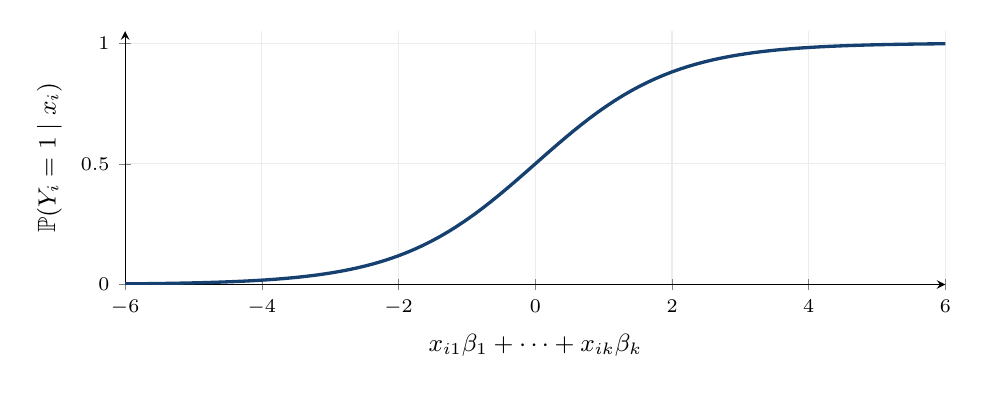
\begin{tikzpicture}
\begin{axis}[base,width=12cm,height=4.8cm,xmin=-6,xmax=6,ymin=0,ymax=1.05,xlabel={$x_{i1}\beta_1+\cdots+x_{ik}\beta_k$},ylabel={$\Prob(Y_i=1\mid x_i)$}]
\addplot[azul,very thick,domain=-6:6]{1/(1+exp(-x))};
\end{axis}
\end{tikzpicture}
\end{center}
\clearpage
\setcounter{tocdepth}{1}
\tableofcontents

\clearpage
\section{Qué se observa y qué se intenta explicar}\label{logit1}
Una observación contiene los datos $x_i$ y $y_i$. Antes de observar la
respuesta, $Y_i$ puede ser cero o uno; después de observarla, $y_i$ es un
número fijo. El vector $x_i=(x_{i1},\ldots,x_{ik})\T$ reúne las características
de esa misma observación. La primera coordenada puede valer uno para todos
los individuos: permite que haya intercepto. El coeficiente $\beta_1$ no
es el dato $x_{i1}$; uno se estima y el otro se conoce.

La afirmación de un modelo es una regla de probabilidad, no una identidad
que obligue a acertar el cero o el uno de cada fila. Condicionar en $x_i$
significa comparar las respuestas posibles manteniendo esas características:
\[
\Prob(Y_i=0\mid x_i)+\Prob(Y_i=1\mid x_i)=1.
\]
Si la probabilidad del uno es $.7$, observar $y_i=0$ sigue siendo posible,
con probabilidad $.3$. Una respuesta cero no demuestra por sí sola que
el modelo sea incorrecto. Para evaluar el modelo se estudian patrones
de muchas respuestas y la calidad de sus probabilidades.

\begin{ejemplo}[Una fila, sin cambiar sus nombres]
Supongamos $x_i=(1,2,1)\T$ y $y_i=0$. Para
$\beta=(0,.3,-.2)\T$, el producto es
\[
x_i\T\beta=(1,2,1)
\begin{pmatrix}0\\.3\\-.2\end{pmatrix}
=1(0)+2(.3)+1(-.2)=.4.
\]
La probabilidad del uno será $e^{.4}/(1+e^{.4})\approx.598688$.
La probabilidad del cero observado será $1/(1+e^{.4})\approx.401312$.
Hay tres coeficientes, pero una sola respuesta en esta observación.
\end{ejemplo}
Las observaciones se apilan en una tabla de $n$ filas.
El modelo puede usar cientos de regresores aunque solo dibujemos dos.
La fórmula conserva el índice $i$ para saber de qué individuo hablamos:
\[
x_{i1}\beta_1+x_{i2}\beta_2+\cdots+x_{ik}\beta_k
=\sum_{j=1}^kx_{ij}\beta_j.
\]
Esta igualdad suma características dentro de una fila.
Una suma $\sum_{i=1}^n$ tiene otro significado: agrega observaciones.
Cambiar el índice de una suma cambia el objeto que se está calculando.

La estimación buscará un único vector de coeficientes compartido por todas
las filas. Cada individuo obtiene una probabilidad distinta a través de sus
propios datos. Tener $n$ probabilidades no significa estimar $n$ interceptos.
Al calcular derivadas respecto de $\beta_j$, los datos $x_{ij}$ y $y_i$
permanecen fijos. Esa separación será esencial en cada regla de la cadena.

\clearpage
\section{Probabilidad condicional y distribución Bernoulli}\label{logit2}
El cociente $\Prob(A\mid B)=\Prob(A\cap B)/\Prob(B)$, para
$\Prob(B)>0$, expresa la probabilidad de $A$ cuando sabemos que ocurrió $B$.
En una regresión, la distribución condicional de $Y_i$ se fija para cada
patrón $x_i$. Para una respuesta binaria hay únicamente dos posibilidades.

Con $\Prob(Y_i=1\mid x_i)$ estrictamente entre cero y uno,
la probabilidad de un dato se escribe sin separar los dos casos:
\[
\Prob(Y_i=y_i\mid x_i)
=\{\Prob(Y_i=1\mid x_i)\}^{y_i}
\{1-\Prob(Y_i=1\mid x_i)\}^{1-y_i},
\quad y_i\in\{0,1\}.
\]
Veamos por qué funciona. Para $y_i=1$, el segundo exponente es cero y
la expresión queda $\Prob(Y_i=1\mid x_i)$. Para $y_i=0$, el primero
es cero y queda $1-\Prob(Y_i=1\mid x_i)$.
No se multiplican las probabilidades de que una misma respuesta sea
simultáneamente cero y uno: los exponentes seleccionan el caso observado.

\begin{deduccion}
La esperanza condicional se calcula sumando valor por probabilidad:
\[
\E[Y_i\mid x_i]
=0\{1-\Prob(Y_i=1\mid x_i)\}
+1\Prob(Y_i=1\mid x_i)=\Prob(Y_i=1\mid x_i).
\]
Como $0^2=0$ y $1^2=1$, también
$\E[Y_i^2\mid x_i]=\Prob(Y_i=1\mid x_i)$. Restar el cuadrado de la media da
\[
\Var(Y_i\mid x_i)
=\Prob(Y_i=1\mid x_i)-\{\Prob(Y_i=1\mid x_i)\}^2
=\Prob(Y_i=1\mid x_i)\{1-\Prob(Y_i=1\mid x_i)\}.
\]
\end{deduccion}
Esta es una propiedad de Bernoulli; todavía no hemos especificado cómo
depende la probabilidad de los regresores. Cuando usemos la regla logística,
la misma probabilidad aparecerá tanto en la media como en la varianza.

\begin{ejemplo}[Dos probabilidades y dos dispersiones]
Si $\Prob(Y_i=1\mid x_i)=.5$, la varianza es $.25$.
Si vale $.9$, la varianza es $.09$.
En ambos casos el dato puede ser cero o uno, pero la segunda distribución
está más concentrada cerca del uno.
\end{ejemplo}
La mayor varianza Bernoulli se obtiene completando un cuadrado:
\[
\Prob(Y_i=1\mid x_i)\{1-\Prob(Y_i=1\mid x_i)\}
=\frac14-\left(\Prob(Y_i=1\mid x_i)-\frac12\right)^2\le\frac14.
\]
La varianza es cero en los extremos de probabilidad cero o uno.
El Logit con coeficientes finitos no llega exactamente a esos extremos,
pero puede acercarse tanto como permita el producto de los datos
y los coeficientes. La disminución de esta varianza también disminuirá
la curvatura que usa Newton.

\clearpage
\section{Exponencial y logaritmo antes de construir el modelo}\label{logit3}
La función exponencial puede definirse por la serie convergente
$e^t=\sum_{r=0}^{\infty}t^r/r!$. Derivar término a término en intervalos
acotados permite comprobar
\[
\frac{\dd e^t}{\dd t}
=\sum_{r=1}^{\infty}\frac{rt^{r-1}}{r!}
=\sum_{r=1}^{\infty}\frac{t^{r-1}}{(r-1)!}=e^t.
\]
Además, $e^t>0$ para todo $t\in\R$.
El logaritmo natural es su inversa sobre $(0,\infty)$:
$\log(e^t)=t$ y $e^{\log u}=u$ para $u>0$.
Diferenciar $e^{\log u}=u$ mediante la cadena da
$e^{\log u}\,\dd(\log u)/\dd u=1$, luego
$\dd(\log u)/\dd u=1/u$.

\textbf{Operaciones de productos.}
La exponencial convierte sumas en productos:
$e^{t+s}=e^te^s$. Aplicar la inversa demuestra
$\log(uv)=\log u+\log v$.
Asimismo, $\log(u/v)=\log u-\log v$ y
$\log(u^c)=c\log u$ para $u>0$.
Estas identidades explican cómo un producto de probabilidades se
convierte en una suma que puede derivarse observación por observación.

\begin{ejemplo}[Por qué se usa un logaritmo]
Diez sucesos independientes con probabilidades $.1$ producen
probabilidad conjunta $10^{-10}$.
Su logaritmo es $10\log(.1)\approx-23.02585$.
Maximizar el producto o su logaritmo selecciona el mismo punto porque
la función logarítmica es estrictamente creciente.
No cambia el problema de optimización; cambia su expresión numérica.
\end{ejemplo}
Para una función diferenciable $u(\beta_j)>0$,
\[
\frac{\partial}{\partial\beta_j}\log u(\beta_j)
=\frac1{u(\beta_j)}\frac{\partial u}{\partial\beta_j}.
\]
Para $u(\beta_j)=1+e^{\sum_{h=1}^kx_{ih}\beta_h}$,
hay tres eslabones:
\[
\frac{\partial}{\partial\beta_j}\log(1+e^{\sum_hx_{ih}\beta_h})
=\frac1{1+e^{\sum_hx_{ih}\beta_h}}
e^{\sum_hx_{ih}\beta_h}
\frac{\partial}{\partial\beta_j}\sum_hx_{ih}\beta_h
=\frac{e^{\sum_hx_{ih}\beta_h}}{1+e^{\sum_hx_{ih}\beta_h}}x_{ij}.
\]
El índice $h$ recorre la suma interna y $j$ identifica el coeficiente
respecto del que derivamos. Se ha escrito el dato $x_{ij}$ explícitamente.

La identidad $\log(1+e^t)\approx t$ para $t$ grande y positivo no se
usará como igualdad exacta. En el cálculo estable se reescribe la misma
función de modo que ninguna exponencial intermedia desborde.
Una buena implementación respeta la expresión matemática aun cuando
la evalúe con operaciones equivalentes.

\begin{figure}[H]\centering
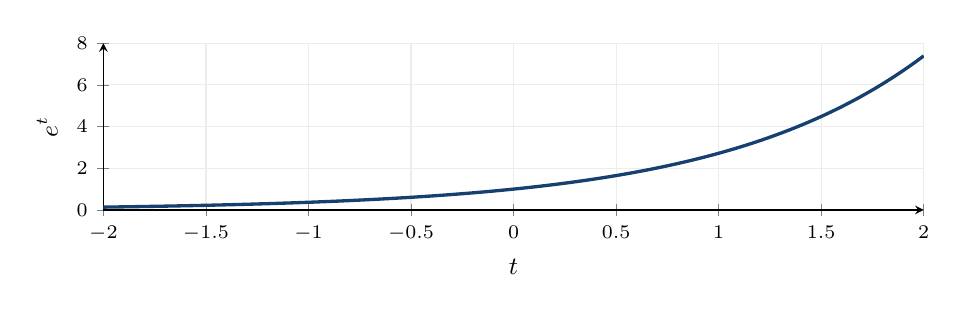
\begin{tikzpicture}
\begin{axis}[base,width=12cm,height=3.7cm,xmin=-2,xmax=2,ymin=0,ymax=8,xlabel={$t$},ylabel={$e^t$}]
\addplot[azul,very thick,domain=-2:2]{exp(x)};
\end{axis}
\end{tikzpicture}
\caption{La exponencial es positiva; el logaritmo convierte productos positivos en sumas.}
\end{figure}

\clearpage
\section{De los odds a la probabilidad logística}\label{logit4}
Los odds comparan éxito con fracaso:
\[
\frac{\Prob(Y_i=1\mid x_i)}{\Prob(Y_i=0\mid x_i)}
=\frac{\Prob(Y_i=1\mid x_i)}{1-\Prob(Y_i=1\mid x_i)}.
\]
Proponemos que el logaritmo de esa razón sea lineal en los regresores:
\[
\log\frac{\Prob(Y_i=1\mid x_i)}{1-\Prob(Y_i=1\mid x_i)}
=x_{i1}\beta_1+\cdots+x_{ik}\beta_k.
\]
Ahora despejamos, sin introducir una letra para el producto lineal.
Exponentiar ambos lados y multiplicar por el denominador da
\[
\begin{aligned}
\frac{\Prob(Y_i=1\mid x_i)}{1-\Prob(Y_i=1\mid x_i)}
&=e^{\sum_{j=1}^kx_{ij}\beta_j},\\
\Prob(Y_i=1\mid x_i)
&=e^{\sum_jx_{ij}\beta_j}
-e^{\sum_jx_{ij}\beta_j}\Prob(Y_i=1\mid x_i),\\
\Prob(Y_i=1\mid x_i)(1+e^{\sum_jx_{ij}\beta_j})
&=e^{\sum_jx_{ij}\beta_j}.
\end{aligned}
\]
El denominador es estrictamente positivo, por tanto
\[
\boxed{\Prob(Y_i=1\mid x_i)=
\frac{e^{\sum_jx_{ij}\beta_j}}{1+e^{\sum_jx_{ij}\beta_j}}
=\frac1{1+e^{-\sum_jx_{ij}\beta_j}}}.
\]
Para verificar la segunda expresión se dividen numerador y denominador
de la primera entre $e^{\sum_jx_{ij}\beta_j}$.
La probabilidad del cero es $1/(1+e^{\sum_jx_{ij}\beta_j})$;
sumarlas produce uno exactamente.

\textbf{Límites y monotonicidad.}
Si el producto lineal tiende a $+\infty$, la probabilidad tiende a uno.
Si tiende a $-\infty$, tiende a cero.
Cuando el producto es cero, la probabilidad es $1/2$.
Todos los coeficientes finitos y todos los datos finitos producen
probabilidades estrictamente entre cero y uno.

\begin{ejemplo}[Odds no es probabilidad]
Si la probabilidad inicial es $.2$, los odds son $.2/.8=.25$.
Multiplicarlos por dos produce odds $.5$.
Despejar la nueva probabilidad da $.5/(1+.5)=1/3$,
no $.4$. El cambio es $1/3-1/5=2/15$.
\end{ejemplo}
Una unidad adicional en $x_{ij}$, manteniendo las otras columnas fijas,
suma $\beta_j$ al logaritmo de los odds.
Por eso los odds se multiplican por $e^{\beta_j}$.
El cambio de probabilidad depende también de todos los datos de la fila:
hay que comparar dos fracciones logísticas distintas.
Con cuadrados o interacciones, cambiar una variable original cambia
varias columnas; ese caso se desarrollará por separado.

\clearpage
\section{Primera derivada logística: cociente y cadena completos}\label{logit5}
Para derivar la probabilidad respecto de $\beta_j$, mantenemos fijos
$x_{i1},\ldots,x_{ik}$. El producto lineal tiene derivada
\[
\frac{\partial}{\partial\beta_j}
(x_{i1}\beta_1+\cdots+x_{ik}\beta_k)=x_{ij}.
\]
La regla del cociente se deduce de derivar $u/v=u\,v^{-1}$:
$(u/v)'=u'/v-uv'/v^2=(u'v-uv')/v^2$.
Aplicarla aquí produce
\[
\begin{aligned}
\frac{\partial}{\partial\beta_j}
\frac{e^{\sum_hx_{ih}\beta_h}}{1+e^{\sum_hx_{ih}\beta_h}}
&=\frac{
e^{\sum_hx_{ih}\beta_h}x_{ij}(1+e^{\sum_hx_{ih}\beta_h})
-e^{\sum_hx_{ih}\beta_h}e^{\sum_hx_{ih}\beta_h}x_{ij}}
{(1+e^{\sum_hx_{ih}\beta_h})^2}\\
&=\frac{e^{\sum_hx_{ih}\beta_h}x_{ij}
+e^{2\sum_hx_{ih}\beta_h}x_{ij}
-e^{2\sum_hx_{ih}\beta_h}x_{ij}}
{(1+e^{\sum_hx_{ih}\beta_h})^2}\\
&=\boxed{\frac{e^{\sum_hx_{ih}\beta_h}}
{(1+e^{\sum_hx_{ih}\beta_h})^2}x_{ij}}.
\end{aligned}
\]
La cancelación del segundo y tercer término es la razón por la que
queda una expresión sencilla. La derivada conserva el signo de $x_{ij}$,
pues el factor exponencial dividido por el cuadrado es positivo.

\textbf{Derivar respecto de un dato.}
Si $x_{ij}$ entra únicamente como una columna lineal, entonces
\[
\frac{\partial\Prob(Y_i=1\mid x_i)}{\partial x_{ij}}
=\frac{e^{\sum_hx_{ih}\beta_h}}
{(1+e^{\sum_hx_{ih}\beta_h})^2}\beta_j.
\]
La primera derivada anterior usa $x_{ij}$, porque se cambia el
coeficiente. Esta segunda usa $\beta_j$, porque se cambia el dato.
Intercambiarlas sería un error de regla de la cadena.

\begin{ejemplo}[La misma fila y dos preguntas diferentes]
Con $x_i=(1,2,1)\T$ y $\beta=(0,.3,-.2)\T$, el producto vale $.4$ y
$e^{.4}/(1+e^{.4})^2\approx.24026075$. Así,
\[
\frac{\partial\Prob(Y_i=1\mid x_i)}{\partial\beta_2}
\approx2(.24026075)=.48052149,
\quad
\frac{\partial\Prob(Y_i=1\mid x_i)}{\partial x_{i2}}
\approx.3(.24026075)=.07207822.
\]
Son cambios locales respecto de argumentos distintos.
\end{ejemplo}
Un incremento pequeño $\delta$ de $\beta_j$ cambia la probabilidad
aproximadamente en la primera derivada por $\delta$.
El resto del desarrollo no se sustituye por una igualdad: se puede
controlar usando la segunda derivada y Taylor.
Cuando $\delta$ es grande, hay que recalcular la fracción logística.

\clearpage
\section{Segunda derivada de la probabilidad y punto de inflexión}\label{logit6}
Derivemos de nuevo respecto de $\beta_l$.
La primera derivada contiene
$e^{\sum_hx_{ih}\beta_h}(1+e^{\sum_hx_{ih}\beta_h})^{-2}x_{ij}$.
El dato $x_{ij}$ permanece fijo.
La regla del producto, la potencia negativa y la cadena dan
\[
\begin{aligned}
\frac{\partial^2\Prob(Y_i=1\mid x_i)}
{\partial\beta_j\partial\beta_l}
={}&x_{ij}x_{il}\left[
\frac{e^{\sum_hx_{ih}\beta_h}}{(1+e^{\sum_hx_{ih}\beta_h})^2}
-\frac{2e^{2\sum_hx_{ih}\beta_h}}{(1+e^{\sum_hx_{ih}\beta_h})^3}
\right]\\
={}&\frac{e^{\sum_hx_{ih}\beta_h}(1-e^{\sum_hx_{ih}\beta_h})}
{(1+e^{\sum_hx_{ih}\beta_h})^3}x_{ij}x_{il}.
\end{aligned}
\]
El primer término proviene de derivar la exponencial del numerador.
El segundo proviene de derivar el denominador elevado a $-2$.
Ponerlos sobre el mismo denominador produce
$e^{\sum_hx_{ih}\beta_h}(1+e^{\sum_hx_{ih}\beta_h})
-2e^{2\sum_hx_{ih}\beta_h}$.

Para el producto lineal escalar, la segunda derivada de la curva
logística tiene el signo de $1-e^{\sum_hx_{ih}\beta_h}$.
La curva es convexa en el lado negativo y cóncava en el positivo.
En cero, la segunda derivada es cero y la primera es $1/4$.
Este punto es una inflexión de la \emph{probabilidad}; no implica
que la log-verosimilitud deje de ser cóncava.

\begin{ejemplo}[Una derivada cruzada puede ser negativa por los datos]
Si el producto lineal es negativo y $x_{ij}x_{il}<0$,
el factor de la curva es positivo pero la derivada cruzada es negativa.
Si $x_{ij}x_{il}=0$, la derivada cruzada es cero.
El signo de una derivada respecto de dos coeficientes combina
curvatura de la función y estructura de la fila.
\end{ejemplo}
La Hessiana de una probabilidad individual puede tener signos positivos
o negativos. La Hessiana de la log-verosimilitud tiene otra forma:
será una suma negativa de productos exteriores ponderados.
Son funciones distintas y se derivan de manera distinta.
Confundirlas es una fuente frecuente de conclusiones equivocadas
sobre la existencia de un máximo.

\begin{figure}[H]\centering
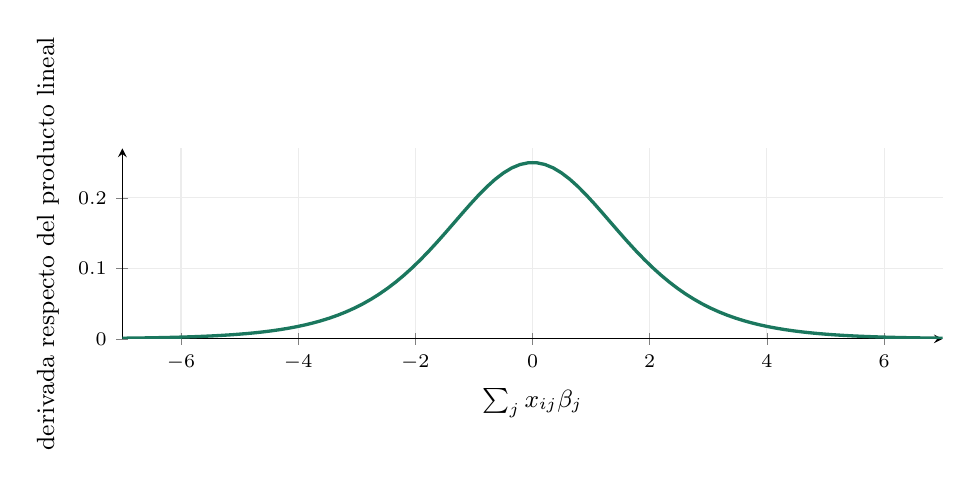
\begin{tikzpicture}
\begin{axis}[base,width=12cm,height=4cm,xmin=-7,xmax=7,ymin=0,ymax=.27,xlabel={$\sum_jx_{ij}\beta_j$},ylabel={derivada respecto del producto lineal}]
\addplot[verde,very thick,domain=-7:7]{exp(-x)/(1+exp(-x))^2};
\end{axis}
\end{tikzpicture}
\caption{Pendiente logística: es máxima en el centro y pequeña en ambos extremos.}
\end{figure}

\clearpage
\section{Construir la matriz de datos fila por fila}\label{logit7}
Cada observación tiene $k$ coordenadas. La matriz $X$ reúne sus
transpuestas como filas, y no como columnas:
\[
x_i=\begin{pmatrix}x_{i1}\\x_{i2}\\\vdots\\x_{ik}\end{pmatrix},
\quad
X=\begin{pmatrix}
x_{11}&x_{12}&\cdots&x_{1k}\\
x_{21}&x_{22}&\cdots&x_{2k}\\
\vdots&\vdots&\ddots&\vdots\\
x_{n1}&x_{n2}&\cdots&x_{nk}
\end{pmatrix}.
\]
$x_i$ tiene $k$ filas y una columna; $X$ tiene $n$ filas y $k$ columnas.
El dato $x_{23}$ es un número: pertenece a la observación dos y a
la característica tres. El vector $x_2$ es toda la segunda observación.
La tercera columna reúne una característica a través de individuos
diferentes. Ninguno de estos tres objetos tiene el mismo tamaño.

\textbf{Producto por los coeficientes.}
El producto $X\beta$ existe porque las $k$ columnas de $X$ coinciden
con las $k$ filas de $\beta$:
\[
X\beta=
\begin{pmatrix}
x_{11}\beta_1+\cdots+x_{1k}\beta_k\\
x_{21}\beta_1+\cdots+x_{2k}\beta_k\\
\vdots\\x_{n1}\beta_1+\cdots+x_{nk}\beta_k
\end{pmatrix}\in\R^{n\times1}.
\]
No se obtiene un coeficiente nuevo por cada fila. El mismo vector
$\beta$ se multiplica por datos diferentes.

\begin{ejemplo}[Tres observaciones y tres coeficientes]
\[
X=\begin{pmatrix}1&-2&0\\1&-1&1\\1&0&0\end{pmatrix},
\quad
\beta=\begin{pmatrix}.2\\.4\\-.3\end{pmatrix},
\quad
X\beta=\begin{pmatrix}.2-2(.4)+0(-.3)\\.2-.4-.3\\.2\end{pmatrix}
=\begin{pmatrix}-.6\\-.5\\.2\end{pmatrix}.
\]
Las tres probabilidades son las fracciones logísticas evaluadas en
$-.6,-.5,.2$, no esos tres números directamente.
\end{ejemplo}
La primera columna de unos produce un desplazamiento común de todos
los productos lineales al cambiar $\beta_1$.
Las otras columnas pueden aumentar algunos productos y disminuir otros,
según los signos de sus datos.
Esta estructura explica por qué una corrección conjunta de los
coeficientes afecta simultáneamente a todas las observaciones.

En el caso de dos regresores más intercepto, usaremos siempre
$x_{i1}=1$, $x_{i2}$ y $x_{i3}$. No se rebautizan los dos regresores.
El dato observado sigue siendo $y_i$.
En tablas numéricas, el encabezado mostrará exactamente esas coordenadas:
las cifras representan valores de $x_{i2}$ y $x_{i3}$.

Al agregar una interacción se agrega una columna calculada con
los mismos datos. Por ejemplo, $x_{i4}=x_{i2}x_{i3}$.
Esta relación se explicará cuando corresponda, porque las derivadas
respecto de una variable original deberán seguir ambas rutas.
La dimensión $k$ cuenta todas las columnas que tienen coeficientes.

\clearpage
\section{Transponer y multiplicar: cada suma del producto}\label{logit8}
Transponer intercambia filas y columnas:
\[
X\T=\begin{pmatrix}
x_{11}&x_{21}&\cdots&x_{n1}\\
x_{12}&x_{22}&\cdots&x_{n2}\\
\vdots&\vdots&\ddots&\vdots\\
x_{1k}&x_{2k}&\cdots&x_{nk}
\end{pmatrix}\in\R^{k\times n}.
\]
Por ello, $(X\T)_{ji}=x_{ij}$. Es el mismo dato, en otra posición.
El producto $X\T y$ tiene $k$ filas, porque multiplica una matriz
$k\times n$ por una columna $n\times1$:
\[
X\T y=
\begin{pmatrix}
x_{11}y_1+x_{21}y_2+\cdots+x_{n1}y_n\\
x_{12}y_1+x_{22}y_2+\cdots+x_{n2}y_n\\
\vdots\\x_{1k}y_1+x_{2k}y_2+\cdots+x_{nk}y_n
\end{pmatrix}
=\begin{pmatrix}\sum_i x_{i1}y_i\\\sum_i x_{i2}y_i\\
\vdots\\\sum_i x_{ik}y_i\end{pmatrix}.
\]
Una fila del primer factor se enfrenta con una columna del segundo.
La suma usa el índice de observación $i$, no el índice de coeficiente.

\begin{ejemplo}[Un producto con ceros que se pueden rastrear]
\[
X=\begin{pmatrix}1&-2&0\\1&-1&1\\1&0&0\end{pmatrix},
\quad y=\begin{pmatrix}0\\0\\1\end{pmatrix},
\quad
X\T y=
\begin{pmatrix}1(0)+1(0)+1(1)\\
-2(0)-1(0)+0(1)\\0(0)+1(0)+0(1)\end{pmatrix}
=\begin{pmatrix}1\\0\\0\end{pmatrix}.
\]
La fila con $y_i=1$ contribuye su vector $x_i$; las otras no contribuyen
a este producto particular. En el score sí contribuirán las tres, porque
allí se restan probabilidades además de usar $y_i$.
\end{ejemplo}
\textbf{Producto interno y exterior.}
Para una misma fila,
\[
x_i\T\beta=\sum_jx_{ij}\beta_j\in\R,\qquad
x_ix_i\T=(x_{ij}x_{il})_{j,l=1}^k\in\R^{k\times k}.
\]
El primero es escalar. El segundo es una matriz y conserva todos
los productos entre coordenadas.
Con $x_i=(1,-2,1)\T$,
\[
x_ix_i\T=
\begin{pmatrix}1\\-2\\1\end{pmatrix}(1,-2,1)
=\begin{pmatrix}1&-2&1\\-2&4&-2\\1&-2&1\end{pmatrix}.
\]
Cada dato puede aportar una matriz completa a la Hessiana.
No se puede sustituir esa matriz por el número $x_i\T x_i=6$,
que solo suma sus términos diagonales.
La distinción también será necesaria al calcular covarianzas entre
componentes del score.

\clearpage
\section{Desplegar completamente el producto X transpuesta por X}\label{logit9}
La entrada $(j,l)$ del producto se obtiene multiplicando la fila $j$
de $X\T$ por la columna $l$ de $X$:
\[
(X\T X)_{jl}
=(X\T)_{j1}X_{1l}+\cdots+(X\T)_{jn}X_{nl}
=x_{1j}x_{1l}+\cdots+x_{nj}x_{nl}.
\]
En consecuencia,
\[
X\T X=
\begin{pmatrix}
\sum_i x_{i1}^2&\sum_i x_{i1}x_{i2}&\cdots&\sum_i x_{i1}x_{ik}\\
\sum_i x_{i2}x_{i1}&\sum_i x_{i2}^2&\cdots&\sum_i x_{i2}x_{ik}\\
\vdots&\vdots&\ddots&\vdots\\
\sum_i x_{ik}x_{i1}&\sum_i x_{ik}x_{i2}&\cdots&\sum_i x_{ik}^2
\end{pmatrix}.
\]
No damos otro nombre a esta matriz. Sus entradas son productos de los
datos y se muestran cuando se utilizan.
La entrada $(j,l)$ coincide con $(l,j)$ porque la multiplicación
de escalares conmuta: $x_{ij}x_{il}=x_{il}x_{ij}$.

Con intercepto y dos regresores, $x_{i1}=1$,
\[
X\T X=
\begin{pmatrix}
n&\sum_i x_{i2}&\sum_i x_{i3}\\
\sum_i x_{i2}&\sum_i x_{i2}^2&\sum_i x_{i2}x_{i3}\\
\sum_i x_{i3}&\sum_i x_{i2}x_{i3}&\sum_i x_{i3}^2
\end{pmatrix}.
\]
La primera entrada es $n$ porque suma $1^2$ una vez por observación.
La entrada $(2,3)$ agrega productos entre las dos características del
mismo individuo; no multiplica sus medias.

\begin{ejemplo}[Todas las entradas, con tres filas]
Para las filas $(1,-2,0),(1,-1,1),(1,0,0)$,
\[
\begin{aligned}
\sum_i1^2&=1+1+1=3,&\sum_i x_{i2}&=-2-1+0=-3,\\
\sum_i x_{i3}&=0+1+0=1,&\sum_i x_{i2}^2&=4+1+0=5,\\
\sum_i x_{i2}x_{i3}&=(-2)0+(-1)1+0(0)=-1,&
\sum_i x_{i3}^2&=0+1+0=1.
\end{aligned}
\]
Así,
$X\T X=\begin{psmallmatrix}3&-3&1\\-3&5&-1\\1&-1&1\end{psmallmatrix}$.
Multiplicar directamente las dos matrices reproduce las nueve entradas.
\end{ejemplo}
También
$X\T X=\sum_i x_ix_i\T$.
Esta última igualdad organiza el cálculo por observaciones;
la matriz anterior lo organiza por pares de columnas.
Ambas son la misma suma, con los índices agrupados de modo distinto.
La Hessiana Logit usará estos mismos productos, pero con un factor
de varianza Bernoulli que cambia en cada iteración.
No será una matriz constante como el producto no ponderado.

\clearpage
\section{Producto exterior, positividad y rango del diseño}\label{logit10}
Para cualquier columna $v=(v_1,\ldots,v_k)\T$,
\[
\begin{aligned}
v\T X\T Xv
&=(Xv)\T(Xv)\\
&=\sum_{i=1}^n(x_{i1}v_1+\cdots+x_{ik}v_k)^2\\
&=\sum_i\sum_j\sum_l x_{ij}x_{il}v_jv_l\ge0.
\end{aligned}
\]
La primera igualdad usa $(Xv)\T=v\T X\T$.
La segunda identifica la suma de cuadrados de una columna.
La tercera abre cada cuadrado en todos sus términos.
La no negatividad no depende de los signos de los datos.

Una matriz simétrica es definida positiva cuando la forma cuadrática
es positiva para todo $v\ne0$.
Aquí sucede exactamente cuando $Xv=0$ implica $v=0$.
Eso significa que ninguna combinación no trivial de columnas del diseño
se anula; las columnas son linealmente independientes y $\rank(X)=k$.

\begin{ejemplo}[Una dependencia que impide identificar pendientes]
Si $x_{i3}=2x_{i2}$ en todas las filas, para $v=(0,-2,1)\T$,
\[
Xv=\begin{pmatrix}
-2x_{12}+x_{13}\\\vdots\\-2x_{n2}+x_{n3}
\end{pmatrix}=0.
\]
El producto lineal del modelo es
$\beta_1+x_{i2}(\beta_2+2\beta_3)$.
Los datos identifican la suma $\beta_2+2\beta_3$,
pero no cada pendiente por separado.
La curva logística no puede recuperar información que el diseño no contiene.
\end{ejemplo}
\textbf{Intercepto y dummies.}
Si una variable categórica tiene dos estados y se incluyen ambos
indicadores junto con la columna de unos, las tres columnas cumplen
$1=x_{i2}+x_{i3}$.
El vector $(1,-1,-1)\T$ pertenece al núcleo de $X$.
Omitir un indicador elige una referencia y elimina esa dependencia
cuando las demás columnas no introducen otra.

La misma comprobación se aplica a productos ponderados positivos:
\[
v\T\left[\sum_i
\frac{e^{\sum_jx_{ij}\beta_j}}{(1+e^{\sum_jx_{ij}\beta_j})^2}
x_ix_i\T\right]v
=\sum_i
\frac{e^{\sum_jx_{ij}\beta_j}}{(1+e^{\sum_jx_{ij}\beta_j})^2}
\left(\sum_jx_{ij}v_j\right)^2.
\]
Para datos y coeficientes finitos, todos los factores son positivos.
La suma vale cero exactamente en el núcleo de $X$.
Por eso rango completo hará que la Hessiana del Logit sea
definida negativa en cada punto finito.
Todavía no demuestra que exista un máximo finito: una función estrictamente
cóncava puede acercarse a su supremo sin alcanzarlo.

\clearpage
\section{Esperanza y covarianza de las respuestas, con índices abiertos}\label{logit11}
Ahora condicionamos en toda la tabla $X$.
El modelo supone que $Y_1,\ldots,Y_n$ son independientes dado $X$,
y que la distribución de cada respuesta depende de su propia fila.
Para $i\ne h$, independencia condicional implica
\[
\E[Y_iY_h\mid X]=\E[Y_i\mid X]\E[Y_h\mid X],
\qquad \Cov(Y_i,Y_h\mid X)=0.
\]
La diagonal de la covarianza se calcula con la distribución Bernoulli.
Por tanto, para el vector de respuestas,
\[
\E[Y\mid X]=
\begin{pmatrix}
\frac{e^{\sum_jx_{1j}\beta_j}}{1+e^{\sum_jx_{1j}\beta_j}}\\
\vdots\\
\frac{e^{\sum_jx_{nj}\beta_j}}{1+e^{\sum_jx_{nj}\beta_j}}
\end{pmatrix},
\]
\[
\Cov(Y\mid X)=
\diag\left(
\frac{e^{\sum_jx_{1j}\beta_j}}{(1+e^{\sum_jx_{1j}\beta_j})^2},
\ldots,
\frac{e^{\sum_jx_{nj}\beta_j}}{(1+e^{\sum_jx_{nj}\beta_j})^2}
\right).
\]
La matriz tiene $n$ filas y $n$ columnas porque describe todas las
covarianzas entre respuestas, no entre coeficientes.

\textbf{La varianza de una suma debe incluir pares.}
Para constantes $c_i$,
\[
\Var\!\left(\sum_i c_iY_i\mid X\right)
=\sum_i c_i^2\Var(Y_i\mid X)
+2\sum_{i<h}c_ic_h\Cov(Y_i,Y_h\mid X).
\]
La última suma desaparece bajo independencia condicional.
Si las respuestas comparten un grupo o un shock, puede no desaparecer.
No basta que cada respuesta marginal siga siendo Bernoulli.

\begin{ejemplo}[Dos respuestas con la misma probabilidad]
Con dos Bernoulli independientes de probabilidad $.5$,
$\Var(Y_1+Y_2\mid X)=.25+.25=.5$.
Si en cambio $Y_1=Y_2$ casi seguramente,
la suma es $2Y_1$ y la varianza es $4(.25)=1$.
La media sigue siendo uno en ambos casos.
\end{ejemplo}
Si las filas de $X$ son aleatorias y comparten factores, la
independencia condicional no significa independencia sin condicionar.
La ley de covarianza total es
\[
\Cov(Y_i,Y_h)=\E[\Cov(Y_i,Y_h\mid X)]
+\Cov(\E[Y_i\mid X],\E[Y_h\mid X]).
\]
El segundo término puede ser no nulo aunque el primero sea cero.
Al usar errores estándar por clúster se analizarán precisamente
los productos cruzados entre contribuciones de un mismo grupo.
Se debe identificar siempre sobre qué información se condiciona.

\clearpage
\section{Por qué un modelo lineal de probabilidad tiene otra geometría}\label{logit12}
Un modelo lineal de probabilidad propone
$\E[Y_i\mid x_i]=\sum_jx_{ij}\beta_j$.
Para una Bernoulli, esa media es una probabilidad, y debe permanecer
en $[0,1]$. Un producto lineal sin restricciones puede salir del intervalo.
El Logit aplica una transformación que garantiza probabilidades válidas.

Si se definiera el error de un modelo lineal bien especificado como
$Y_i-\sum_jx_{ij}\beta_j$, la esperanza condicional sería cero y
la varianza Bernoulli sería
\[
\Var(Y_i\mid x_i)=
\left(\sum_jx_{ij}\beta_j\right)
\left(1-\sum_jx_{ij}\beta_j\right).
\]
En general varía entre filas: la homocedasticidad no se deduce de
que la respuesta esté codificada con ceros y unos.

\textbf{Mínimos cuadrados no maximiza la verosimilitud Bernoulli.}
Derivar la suma de errores al cuadrado produce
\[
\frac{\partial}{\partial\beta_j}
\sum_i\left(y_i-\sum_lx_{il}\beta_l\right)^2
=-2\sum_i x_{ij}\left(y_i-\sum_lx_{il}\beta_l\right).
\]
Igualar a cero y reunir todas las coordenadas da
\[
\begin{pmatrix}
\sum_i x_{i1}^2&\cdots&\sum_i x_{i1}x_{ik}\\
\vdots&\ddots&\vdots\\
\sum_i x_{ik}x_{i1}&\cdots&\sum_i x_{ik}^2
\end{pmatrix}
\begin{pmatrix}\widehat\beta_1\\\vdots\\\widehat\beta_k\end{pmatrix}
=
\begin{pmatrix}\sum_i x_{i1}y_i\\\vdots\\\sum_i x_{ik}y_i\end{pmatrix}.
\]
La matriz no depende de los coeficientes.
En Logit, reemplazar el producto lineal por una probabilidad logística
produce ecuaciones no lineales; la matriz de curvatura deberá recalcularse.

\begin{ejemplo}[Una recta puede salir del intervalo]
Si la regla lineal es $.2+.3x_{i2}$, en $x_{i2}=4$ predice $1.4$.
La regla logística con ese mismo producto lineal predice
$e^{1.4}/(1+e^{1.4})\approx.802184$.
Estas expresiones no son dos formas de escribir la misma media.
\end{ejemplo}
Un error cuadrático enfatiza distancias verticales al número observado.
La log-verosimilitud Bernoulli enfatiza la probabilidad que se asignó
al resultado efectivamente observado.
Por eso un resultado $y_i=1$ con probabilidad estimada extremadamente
pequeña produce una pérdida logarítmica grande.

MCO e IRLS se relacionarán porque una aproximación cuadrática local
del Logit puede resolverse mediante mínimos cuadrados ponderados.
Esa relación local no transforma el objetivo global del Logit en
la suma de cuadrados original.
Los pesos y las respuestas de trabajo dependerán del punto actual,
y nunca se confundirán con nuevos datos binarios observados.

\clearpage
\section{Verosimilitud: multiplicar las probabilidades observadas}\label{logit13}
Fijemos los datos $X$ y $y$. La independencia condicional permite
multiplicar las probabilidades de cada resultado:
\[
L(\beta;y,X)=\prod_{i=1}^n
\left[\frac{e^{\sum_jx_{ij}\beta_j}}
{1+e^{\sum_jx_{ij}\beta_j}}\right]^{y_i}
\left[\frac1{1+e^{\sum_jx_{ij}\beta_j}}\right]^{1-y_i}.
\]
$L$ es una función del parámetro, con los datos fijados.
No es una distribución de probabilidad sobre $\beta$.
La suma de probabilidades se normaliza sobre respuestas posibles;
al fijar las respuestas y variar $\beta$, se estudia otro objeto.

\textbf{Abrir un producto pequeño.}
Para $n=3$ y $y=(0,1,0)\T$,
\[
L(\beta;y,X)=
\frac1{1+e^{\sum_jx_{1j}\beta_j}}
\frac{e^{\sum_jx_{2j}\beta_j}}{1+e^{\sum_jx_{2j}\beta_j}}
\frac1{1+e^{\sum_jx_{3j}\beta_j}}.
\]
La segunda fila aporta la probabilidad del uno;
la primera y tercera aportan la del cero.
Si dos filas comparten los mismos regresores y tienen respuestas opuestas,
sus dos probabilidades aparecen por separado y ambas importan.

\begin{ejemplo}[Evaluar un parámetro no es estimarlo]
Si los tres productos lineales son $0,1,-1$, las probabilidades
correspondientes al dato $(0,1,0)$ son
$1/2$, $e/(1+e)$ y $1/(1+e^{-1})=e/(1+e)$.
El producto es $\tfrac12[e/(1+e)]^2\approx.267223$.
Otro parámetro produce otras tres probabilidades y otra verosimilitud.
\end{ejemplo}
Como cada factor está entre cero y uno para coeficientes finitos,
$0<L(\beta;y,X)<1$.
Puede acercarse a uno cuando los datos son separables y los
coeficientes crecen sin límite; eso no garantiza que el máximo se alcance.

\textbf{Respuestas con el mismo patrón de datos.}
Si un patrón aparece $m$ veces, con $s$ unos y $m-s$ ceros,
el producto de sus filas contiene
\[
\left[\frac{e^{\sum_jx_{ij}\beta_j}}
{1+e^{\sum_jx_{ij}\beta_j}}\right]^s
\left[\frac1{1+e^{\sum_jx_{ij}\beta_j}}\right]^{m-s}.
\]
Si se observa solamente el conteo, en vez de la secuencia de resultados,
la masa binomial agrega $\binom ms$. Este factor no depende de
$\beta$ y no cambia el maximizador, pero sí la probabilidad numérica
del evento observado. La verosimilitud debe corresponder al dato que
realmente se registró.

Este producto será difícil de diferenciar directamente para $n$ grande.
El siguiente paso convierte cada factor en un sumando sin cambiar
el máximo. Las constantes que dependen de la forma del dato se
mantienen cuando se compara una probabilidad específica.

\clearpage
\section{Log-verosimilitud: abrir todos los logaritmos}\label{logit14}
Aplicar el logaritmo al producto produce una suma:
\[
\ell(\beta;y,X)=\sum_i\left[
y_i\log\frac{e^{\sum_jx_{ij}\beta_j}}{1+e^{\sum_jx_{ij}\beta_j}}
+(1-y_i)\log\frac1{1+e^{\sum_jx_{ij}\beta_j}}
\right].
\]
Ahora abrimos las dos razones usando $\log(u/v)=\log u-\log v$:
\[
\begin{aligned}
\ell(\beta;y,X)
=\sum_i\bigg[&
y_i\sum_jx_{ij}\beta_j
-y_i\log(1+e^{\sum_jx_{ij}\beta_j})\\
&-(1-y_i)\log(1+e^{\sum_jx_{ij}\beta_j})\bigg].
\end{aligned}
\]
Los dos términos de logaritmo comparten la misma función.
Su coeficiente es $-y_i-(1-y_i)=-1$. Por tanto,
\[
\boxed{\ell(\beta;y,X)=
\sum_{i=1}^n\left[
y_i\sum_{j=1}^kx_{ij}\beta_j-
\log(1+e^{\sum_{j=1}^kx_{ij}\beta_j})\right]}.
\]
La desaparición de $y_i$ del coeficiente del segundo término es
una cancelación algebraica, no un supuesto de independencia adicional.

\textbf{Escribir una fila cuando se observó cero.}
Si $y_i=0$,
\[
y_i\sum_jx_{ij}\beta_j-\log(1+e^{\sum_jx_{ij}\beta_j})
=-\log(1+e^{\sum_jx_{ij}\beta_j}).
\]
Es el logaritmo de la probabilidad del cero.
Si $y_i=1$, se obtiene
\[
\sum_jx_{ij}\beta_j-\log(1+e^{\sum_jx_{ij}\beta_j})
=-\log(1+e^{-\sum_jx_{ij}\beta_j}),
\]
porque $1+e^t=e^t(1+e^{-t})$. Es el logaritmo de la probabilidad del uno.

\begin{ejemplo}[El inicio en coeficientes cero]
Con $\beta=0$, todas las filas aportan
$-\log(1+e^0)=-\log2$. Así,
$\ell(0;y,X)=-n\log2$, cualquiera sea la secuencia observada.
Para los doce datos originales, $\ell(0)\approx-8.31776617$.
\end{ejemplo}
Cada sumando es no positivo porque es el logaritmo de una probabilidad
no mayor que uno. La log-verosimilitud total tampoco puede ser positiva.
Esta cota ayudará a probar que una penalización cuadrática
obliga a los coeficientes a permanecer acotados.

Multiplicar la log-verosimilitud por $1/n$ tampoco cambia su maximizador.
Pero cambia sus derivadas por ese factor.
Al invertir una matriz de información debe comprobarse si se está
usando la suma o el promedio: la escala de la covarianza depende
de esa elección. Se desarrollarán ambos cálculos más adelante.

\clearpage
\section{Primera derivada de la log-verosimilitud sin saltar eslabones}\label{logit15}
Derivamos respecto de un coeficiente $\beta_l$.
Los datos $x_{ij}$ y $y_i$ no cambian:
\[
\begin{aligned}
\frac{\partial\ell}{\partial\beta_l}
&=\sum_i\frac{\partial}{\partial\beta_l}
\left[y_i\sum_jx_{ij}\beta_j-
\log(1+e^{\sum_jx_{ij}\beta_j})\right]\\
&=\sum_i\left[
y_i\frac{\partial}{\partial\beta_l}\sum_jx_{ij}\beta_j
-\frac1{1+e^{\sum_jx_{ij}\beta_j}}
\frac{\partial}{\partial\beta_l}e^{\sum_jx_{ij}\beta_j}
\right]\\
&=\sum_i\left[
y_ix_{il}-
\frac1{1+e^{\sum_jx_{ij}\beta_j}}
e^{\sum_jx_{ij}\beta_j}x_{il}\right]\\
&=\boxed{\sum_i x_{il}\left[
y_i-\frac{e^{\sum_jx_{ij}\beta_j}}{1+e^{\sum_jx_{ij}\beta_j}}
\right]}.
\end{aligned}
\]
La contribución del dato es la diferencia entre resultado observado
y probabilidad calculada, multiplicada por su coordenada $x_{il}$.
La suma agrega esas contribuciones a través de observaciones.

\textbf{Leer el signo antes de agregar.}
Si $y_i=1$, la diferencia entre corchetes es positiva.
Si $y_i=0$, es negativa.
Sin embargo, el signo de la contribución completa también depende
de $x_{il}$. Un dato negativo invierte el signo.
La interpretación de la derivada del intercepto es más directa:
allí $x_{i1}=1$ en todas las filas.

\begin{ejemplo}[Una respuesta cero y un regresor negativo]
Para $x_i=(1,-2,0)\T$, $y_i=0$ y coeficientes cero,
la probabilidad es $1/2$. Las tres contribuciones son
\[
1(0-\tfrac12)=-\tfrac12,\quad
-2(0-\tfrac12)=1,\quad
0(0-\tfrac12)=0.
\]
La fila sugiere disminuir el intercepto y aumentar la segunda pendiente,
según el sentido local de la log-verosimilitud.
No determina por sí sola el desplazamiento conjunto óptimo.
\end{ejemplo}
Si se busca un máximo interior finito, las $k$ derivadas deben ser cero:
\[
\sum_i x_{il}\left[y_i-
\frac{e^{\sum_jx_{ij}\widehat\beta_j}}
{1+e^{\sum_jx_{ij}\widehat\beta_j}}\right]=0,
\qquad l=1,\ldots,k.
\]
Estas son ecuaciones no lineales en todos los coeficientes.
La misma fracción depende de cada $\widehat\beta_j$.
No se despeja una pendiente aislada ignorando el resto del vector.

La condición de derivadas cero es necesaria para un máximo interior,
pero no demuestra que exista ese punto.
Primero probaremos concavidad; luego examinaremos qué ocurre cuando
los datos empujan un máximo hacia coeficientes infinitos.

\clearpage
\section{El vector de derivadas y su multiplicación explícita}\label{logit16}
El gradiente de una función escalar de $k$ coeficientes es una columna
de $k$ derivadas. En este problema,
\[
\nabla_\beta\ell=
\begin{pmatrix}
\sum_i x_{i1}\left[y_i-\frac{e^{\sum_jx_{ij}\beta_j}}{1+e^{\sum_jx_{ij}\beta_j}}\right]\\
\sum_i x_{i2}\left[y_i-\frac{e^{\sum_jx_{ij}\beta_j}}{1+e^{\sum_jx_{ij}\beta_j}}\right]\\
\vdots\\
\sum_i x_{ik}\left[y_i-\frac{e^{\sum_jx_{ij}\beta_j}}{1+e^{\sum_jx_{ij}\beta_j}}\right]
\end{pmatrix}.
\]
No asignamos una nueva letra a este vector.
Su nombre funcional indica qué se deriva y cada entrada muestra los datos.

Se puede verificar la construcción multiplicando dos objetos con tamaños
compatibles:
\[
\begin{pmatrix}
x_{11}&\cdots&x_{n1}\\x_{12}&\cdots&x_{n2}\\
\vdots&\ddots&\vdots\\x_{1k}&\cdots&x_{nk}
\end{pmatrix}
\begin{pmatrix}
y_1-\frac{e^{\sum_jx_{1j}\beta_j}}{1+e^{\sum_jx_{1j}\beta_j}}\\
\vdots\\
y_n-\frac{e^{\sum_jx_{nj}\beta_j}}{1+e^{\sum_jx_{nj}\beta_j}}
\end{pmatrix}.
\]
La primera matriz tiene $k$ filas y $n$ columnas.
La segunda columna contiene una diferencia por observación.
Su producto coincide entrada por entrada con el gradiente anterior.

\textbf{Intercepto y dos regresores.}
Con $x_{i1}=1$, las tres sumas son
\[
\begin{aligned}
\frac{\partial\ell}{\partial\beta_1}
&=\sum_i\left[y_i-\frac{e^{\beta_1+x_{i2}\beta_2+x_{i3}\beta_3}}
{1+e^{\beta_1+x_{i2}\beta_2+x_{i3}\beta_3}}\right],\\
\frac{\partial\ell}{\partial\beta_2}
&=\sum_i x_{i2}\left[y_i-\frac{e^{\beta_1+x_{i2}\beta_2+x_{i3}\beta_3}}
{1+e^{\beta_1+x_{i2}\beta_2+x_{i3}\beta_3}}\right],\\
\frac{\partial\ell}{\partial\beta_3}
&=\sum_i x_{i3}\left[y_i-\frac{e^{\beta_1+x_{i2}\beta_2+x_{i3}\beta_3}}
{1+e^{\beta_1+x_{i2}\beta_2+x_{i3}\beta_3}}\right].
\end{aligned}
\]
En la estimación con intercepto, la primera ecuación implica
que la suma de probabilidades ajustadas coincide con la suma de unos
observados, si existe una solución interior.
Las otras ecuaciones equilibran diferencias ponderadas por cada regresor.
Ninguna exige igualdad fila por fila.

Si dos individuos tienen datos iguales y respuestas opuestas,
sus diferencias pueden compensarse. El modelo les asigna la misma
probabilidad y sigue siendo coherente.
El ajuste probabilístico comparte información entre filas y no intenta
interpolar cada respuesta como una función determinista.

\clearpage
\section{Jacobiano de todas las probabilidades respecto de los coeficientes}\label{logit17}
Ahora la función de salida no es escalar: devuelve una probabilidad
para cada fila. Su Jacobiano tiene $n$ filas y $k$ columnas.
La entrada $(i,l)$ es
\[
\frac{\partial\Prob(Y_i=1\mid x_i)}{\partial\beta_l}
=\frac{e^{\sum_jx_{ij}\beta_j}}
{(1+e^{\sum_jx_{ij}\beta_j})^2}x_{il}.
\]
Escribir la matriz completa muestra que no se deriva una probabilidad
respecto de otra probabilidad, sino respecto de cada coeficiente:
\[
\begin{pmatrix}
\frac{e^{\sum_jx_{1j}\beta_j}x_{11}}{(1+e^{\sum_jx_{1j}\beta_j})^2}
&\cdots&
\frac{e^{\sum_jx_{1j}\beta_j}x_{1k}}{(1+e^{\sum_jx_{1j}\beta_j})^2}\\
\vdots&\ddots&\vdots\\
\frac{e^{\sum_jx_{nj}\beta_j}x_{n1}}{(1+e^{\sum_jx_{nj}\beta_j})^2}
&\cdots&
\frac{e^{\sum_jx_{nj}\beta_j}x_{nk}}{(1+e^{\sum_jx_{nj}\beta_j})^2}
\end{pmatrix}.
\]
Cada fila es el vector de datos de esa observación,
multiplicado por la varianza Bernoulli calculada para esa fila.

\textbf{Factor diagonal, sin abreviarlo.}
La matriz puede construirse como
\[
\diag\left(
\frac{e^{\sum_jx_{1j}\beta_j}}{(1+e^{\sum_jx_{1j}\beta_j})^2},
\ldots,
\frac{e^{\sum_jx_{nj}\beta_j}}{(1+e^{\sum_jx_{nj}\beta_j})^2}
\right)X.
\]
Multiplicar por la izquierda con una diagonal multiplica filas.
Por la derecha se multiplicarían columnas, que sería otra operación.

\begin{ejemplo}[Tres filas en coeficientes cero]
Para $X=\begin{psmallmatrix}1&-2&0\\1&-1&1\\1&0&0\end{psmallmatrix}$,
cada factor es $1/4$, de modo que el Jacobiano es
\[
\begin{pmatrix}1/4&0&0\\0&1/4&0\\0&0&1/4\end{pmatrix}
\begin{pmatrix}1&-2&0\\1&-1&1\\1&0&0\end{pmatrix}
=\begin{pmatrix}1/4&-1/2&0\\1/4&-1/4&1/4\\1/4&0&0\end{pmatrix}.
\]
Un cambio en $\beta_2$ afecta con signo negativo las dos primeras
probabilidades y no cambia la tercera a primer orden.
\end{ejemplo}
Para una perturbación $h$ de los coeficientes, la columna de cambios
de probabilidades es aproximadamente este Jacobiano por $h$.
Las dimensiones son $(n\times k)(k\times1)=n\times1$.
El gradiente de una única probabilidad, en cambio, es una columna
de $k$ entradas. La transpuesta de su fila en el Jacobiano produce ese gradiente.

Esta derivada vectorial permitirá deducir de nuevo la Hessiana.
También será la transformación que propaga la covarianza de coeficientes
hacia la covarianza conjunta de probabilidades predichas.

\clearpage
\section{Segunda derivada de la log-verosimilitud paso a paso}\label{logit18}
Partimos de la derivada ya obtenida:
\[
\frac{\partial\ell}{\partial\beta_l}
=\sum_i x_{il}\left[y_i-
\frac{e^{\sum_jx_{ij}\beta_j}}{1+e^{\sum_jx_{ij}\beta_j}}\right].
\]
Derivamos respecto de $\beta_h$. Los dos datos $x_{il}$ y $y_i$
son constantes en esta operación:
\[
\begin{aligned}
\frac{\partial^2\ell}{\partial\beta_l\partial\beta_h}
&=\sum_i x_{il}\left[
0-\frac{\partial}{\partial\beta_h}
\frac{e^{\sum_jx_{ij}\beta_j}}{1+e^{\sum_jx_{ij}\beta_j}}\right]\\
&=-\sum_i x_{il}
\frac{e^{\sum_jx_{ij}\beta_j}x_{ih}
(1+e^{\sum_jx_{ij}\beta_j})
-e^{2\sum_jx_{ij}\beta_j}x_{ih}}
{(1+e^{\sum_jx_{ij}\beta_j})^2}\\
&=\boxed{-\sum_i
\frac{e^{\sum_jx_{ij}\beta_j}}
{(1+e^{\sum_jx_{ij}\beta_j})^2}x_{il}x_{ih}}.
\end{aligned}
\]
El signo negativo proviene de que en el gradiente se resta
la probabilidad. El factor de derivada de la probabilidad es positivo.
Los datos $y_i$ desaparecen de esta segunda derivada
porque no dependen de los coeficientes.

\textbf{Derivada pura.}
Para $h=l$,
\[
\frac{\partial^2\ell}{\partial\beta_l^2}
=-\sum_i\frac{e^{\sum_jx_{ij}\beta_j}}
{(1+e^{\sum_jx_{ij}\beta_j})^2}x_{il}^2\le0.
\]
La desigualdad es estricta si alguna fila tiene $x_{il}\ne0$.
Una derivada pura negativa indica curvatura hacia abajo en esa coordenada.

\textbf{Derivada cruzada.}
Si $h\ne l$, el signo de la suma depende de los productos
$x_{il}x_{ih}$. Puede ser positivo, negativo o cero.
La condición de concavidad exige que la matriz completa tenga
forma cuadrática no positiva; no exige que cada entrada sea negativa.

\begin{ejemplo}[Cruces y diagonal]
En coeficientes cero, para las tres filas
$(1,-2,0),(1,-1,1),(1,0,0)$,
\[
\frac{\partial^2\ell}{\partial\beta_2^2}
=-\tfrac14(4+1+0)=-\tfrac54,\quad
\frac{\partial^2\ell}{\partial\beta_1\partial\beta_2}
=-\tfrac14(-2-1+0)=\tfrac34.
\]
La entrada cruzada es positiva, aunque la Hessiana sea definida negativa
porque esas tres filas son independientes.
\end{ejemplo}
La simetría se comprueba directamente:
$x_{il}x_{ih}=x_{ih}x_{il}$.
Por eso derivar primero en $\beta_l$ y luego en $\beta_h$
produce la misma entrada que hacerlo en el orden inverso.
El resultado también concuerda con la igualdad de derivadas cruzadas
de una función con derivadas continuas.

\clearpage
\section{Derivada pura: coeficientes 1 y 1, con doce filas}\label{logit19}
En esta unidad calculamos una entrada específica de la Hessiana.
El primer índice elige la derivada de la log-verosimilitud; el segundo
elige el coeficiente que vuelve a cambiar.
Se mantienen fijos todos los datos. Con $x_{i1}=1$,
\[
\frac{\partial\ell}{\partial\beta_1}=\sum_{i=1}^{12}1\left[y_i-\frac{e^{\beta_1+x_{i2}\beta_2+x_{i3}\beta_3}}{1+e^{\beta_1+x_{i2}\beta_2+x_{i3}\beta_3}}\right].
\]

El término que contiene $y_i$ tiene derivada cero.
La exponencial tiene derivada igual a sí misma por la coordenada
del coeficiente que se está cambiando. La regla del cociente da
\[
\begin{aligned}
\frac{\partial^2\ell}{\partial\beta_1\partial\beta_1}&=-\sum_{i=1}^{12}\,(1)(1)\frac{e^{\beta_1+x_{i2}\beta_2+x_{i3}\beta_3}(1+e^{\beta_1+x_{i2}\beta_2+x_{i3}\beta_3})-e^{2(\beta_1+x_{i2}\beta_2+x_{i3}\beta_3)}}{(1+e^{\beta_1+x_{i2}\beta_2+x_{i3}\beta_3})^2}\\&=-\sum_{i=1}^{12}\frac{e^{\beta_1+x_{i2}\beta_2+x_{i3}\beta_3}}{(1+e^{\beta_1+x_{i2}\beta_2+x_{i3}\beta_3})^2}\,(1)(1).\end{aligned}
\]

Al comenzar en coeficientes cero, la fracción vale $1/4$ en cada fila.
La tabla abre todos los productos del ejemplo original. La última
columna usa el punto de prueba $(.2,.3,-.1)^\mathsf T$, que se elige
para comparar curvaturas y todavía no es una estimación.
\begin{center}\small
\begin{tabular}{rrrrrr}
\toprule
$i$&$x_{i1}$&$x_{i1}$&$x_{i1}x_{i1}$&Contribución en $0$&En $(.2,.3,-.1)$\\\midrule1&1&1&1&-0.250000&-0.240261\\
2&1&1&1&-0.250000&-0.247517\\
3&1&1&1&-0.250000&-0.247517\\
4&1&1&1&-0.250000&-0.240261\\
5&1&1&1&-0.250000&-0.213910\\
6&1&1&1&-0.250000&-0.196612\\
7&1&1&1&-0.250000&-0.247517\\
8&1&1&1&-0.250000&-0.247517\\
9&1&1&1&-0.250000&-0.244458\\
10&1&1&1&-0.250000&-0.213910\\
11&1&1&1&-0.250000&-0.196612\\
12&1&1&1&-0.250000&-0.158685\\\bottomrule\end{tabular}\end{center}\[
-\frac14\left[(1)+(1)+(1)+(1)+(1)+(1)+(1)+(1)+(1)+(1)+(1)+(1)\right]=-3.00000000.
\]

En el punto de prueba, los doce factores dejan de ser iguales.
Sumar la última columna, calculada internamente sin redondear, da
\[
\left.\frac{\partial^2\ell}{\partial\beta_1\partial\beta_1}\right|_{\beta=(.2,.3,-.1)\T}=-2.69477425.
\]
Al ser una derivada pura, cada producto es un cuadrado no negativo. Cada contribución a la segunda derivada es no positiva.
Las entradas con índices invertidos deben coincidir.
La comprobación se hace multiplicando los mismos datos en el orden
contrario; no requiere volver a ajustar el modelo.
El cambio entre las dos columnas proviene de las probabilidades,
porque la tabla de datos permanece fija.

\clearpage
\section{Derivada cruzada: coeficientes 1 y 2, con doce filas}\label{logit20}
En esta unidad calculamos una entrada específica de la Hessiana.
El primer índice elige la derivada de la log-verosimilitud; el segundo
elige el coeficiente que vuelve a cambiar.
Se mantienen fijos todos los datos. Con $x_{i1}=1$,
\[
\frac{\partial\ell}{\partial\beta_1}=\sum_{i=1}^{12}1\left[y_i-\frac{e^{\beta_1+x_{i2}\beta_2+x_{i3}\beta_3}}{1+e^{\beta_1+x_{i2}\beta_2+x_{i3}\beta_3}}\right].
\]

El término que contiene $y_i$ tiene derivada cero.
La exponencial tiene derivada igual a sí misma por la coordenada
del coeficiente que se está cambiando. La regla del cociente da
\[
\begin{aligned}
\frac{\partial^2\ell}{\partial\beta_1\partial\beta_2}&=-\sum_{i=1}^{12}\,(1)(x_{i2})\frac{e^{\beta_1+x_{i2}\beta_2+x_{i3}\beta_3}(1+e^{\beta_1+x_{i2}\beta_2+x_{i3}\beta_3})-e^{2(\beta_1+x_{i2}\beta_2+x_{i3}\beta_3)}}{(1+e^{\beta_1+x_{i2}\beta_2+x_{i3}\beta_3})^2}\\&=-\sum_{i=1}^{12}\frac{e^{\beta_1+x_{i2}\beta_2+x_{i3}\beta_3}}{(1+e^{\beta_1+x_{i2}\beta_2+x_{i3}\beta_3})^2}\,(1)(x_{i2}).\end{aligned}
\]

Al comenzar en coeficientes cero, la fracción vale $1/4$ en cada fila.
La tabla abre todos los productos del ejemplo original. La última
columna usa el punto de prueba $(.2,.3,-.1)^\mathsf T$, que se elige
para comparar curvaturas y todavía no es una estimación.
\begin{center}\small
\begin{tabular}{rrrrrr}
\toprule
$i$&$x_{i1}$&$x_{i2}$&$x_{i1}x_{i2}$&Contribución en $0$&En $(.2,.3,-.1)$\\\midrule1&1&-2&-2&0.500000&0.480521\\
2&1&-1&-1&0.250000&0.247517\\
3&1&0&0&-0.000000&-0.000000\\
4&1&1&1&-0.250000&-0.240261\\
5&1&2&2&-0.500000&-0.427819\\
6&1&3&3&-0.750000&-0.589836\\
7&1&-1&-1&0.250000&0.247517\\
8&1&0&0&-0.000000&-0.000000\\
9&1&1&1&-0.250000&-0.244458\\
10&1&2&2&-0.500000&-0.427819\\
11&1&3&3&-0.750000&-0.589836\\
12&1&4&4&-1.000000&-0.634740\\\bottomrule\end{tabular}\end{center}\[
-\frac14\left[(-2)+(-1)+(0)+(1)+(2)+(3)+(-1)+(0)+(1)+(2)+(3)+(4)\right]=-3.00000000.
\]

En el punto de prueba, los doce factores dejan de ser iguales.
Sumar la última columna, calculada internamente sin redondear, da
\[
\left.\frac{\partial^2\ell}{\partial\beta_1\partial\beta_2}\right|_{\beta=(.2,.3,-.1)\T}=-2.17921440.
\]
Al ser una derivada cruzada, los productos pueden tener signos diferentes. Su suma no tiene por qué ser positiva: la concavidad se comprueba con la forma cuadrática de la matriz completa, no con el signo de esta entrada.
Las entradas con índices invertidos deben coincidir.
La comprobación se hace multiplicando los mismos datos en el orden
contrario; no requiere volver a ajustar el modelo.
El cambio entre las dos columnas proviene de las probabilidades,
porque la tabla de datos permanece fija.

\clearpage
\section{Derivada cruzada: coeficientes 1 y 3, con doce filas}\label{logit21}
En esta unidad calculamos una entrada específica de la Hessiana.
El primer índice elige la derivada de la log-verosimilitud; el segundo
elige el coeficiente que vuelve a cambiar.
Se mantienen fijos todos los datos. Con $x_{i1}=1$,
\[
\frac{\partial\ell}{\partial\beta_1}=\sum_{i=1}^{12}1\left[y_i-\frac{e^{\beta_1+x_{i2}\beta_2+x_{i3}\beta_3}}{1+e^{\beta_1+x_{i2}\beta_2+x_{i3}\beta_3}}\right].
\]

El término que contiene $y_i$ tiene derivada cero.
La exponencial tiene derivada igual a sí misma por la coordenada
del coeficiente que se está cambiando. La regla del cociente da
\[
\begin{aligned}
\frac{\partial^2\ell}{\partial\beta_1\partial\beta_3}&=-\sum_{i=1}^{12}\,(1)(x_{i3})\frac{e^{\beta_1+x_{i2}\beta_2+x_{i3}\beta_3}(1+e^{\beta_1+x_{i2}\beta_2+x_{i3}\beta_3})-e^{2(\beta_1+x_{i2}\beta_2+x_{i3}\beta_3)}}{(1+e^{\beta_1+x_{i2}\beta_2+x_{i3}\beta_3})^2}\\&=-\sum_{i=1}^{12}\frac{e^{\beta_1+x_{i2}\beta_2+x_{i3}\beta_3}}{(1+e^{\beta_1+x_{i2}\beta_2+x_{i3}\beta_3})^2}\,(1)(x_{i3}).\end{aligned}
\]

Al comenzar en coeficientes cero, la fracción vale $1/4$ en cada fila.
La tabla abre todos los productos del ejemplo original. La última
columna usa el punto de prueba $(.2,.3,-.1)^\mathsf T$, que se elige
para comparar curvaturas y todavía no es una estimación.
\begin{center}\small
\begin{tabular}{rrrrrr}
\toprule
$i$&$x_{i1}$&$x_{i3}$&$x_{i1}x_{i3}$&Contribución en $0$&En $(.2,.3,-.1)$\\\midrule1&1&0&0&-0.000000&-0.000000\\
2&1&1&1&-0.250000&-0.247517\\
3&1&0&0&-0.000000&-0.000000\\
4&1&1&1&-0.250000&-0.240261\\
5&1&0&0&-0.000000&-0.000000\\
6&1&1&1&-0.250000&-0.196612\\
7&1&1&1&-0.250000&-0.247517\\
8&1&0&0&-0.000000&-0.000000\\
9&1&2&2&-0.500000&-0.488917\\
10&1&0&0&-0.000000&-0.000000\\
11&1&1&1&-0.250000&-0.196612\\
12&1&0&0&-0.000000&-0.000000\\\bottomrule\end{tabular}\end{center}\[
-\frac14\left[(0)+(1)+(0)+(1)+(0)+(1)+(1)+(0)+(2)+(0)+(1)+(0)\right]=-1.75000000.
\]

En el punto de prueba, los doce factores dejan de ser iguales.
Sumar la última columna, calculada internamente sin redondear, da
\[
\left.\frac{\partial^2\ell}{\partial\beta_1\partial\beta_3}\right|_{\beta=(.2,.3,-.1)\T}=-1.61743438.
\]
Al ser una derivada cruzada, los productos pueden tener signos diferentes. Su suma no tiene por qué ser positiva: la concavidad se comprueba con la forma cuadrática de la matriz completa, no con el signo de esta entrada.
Las entradas con índices invertidos deben coincidir.
La comprobación se hace multiplicando los mismos datos en el orden
contrario; no requiere volver a ajustar el modelo.
El cambio entre las dos columnas proviene de las probabilidades,
porque la tabla de datos permanece fija.

\clearpage
\section{Derivada cruzada: coeficientes 2 y 1, con doce filas}\label{logit22}
En esta unidad calculamos una entrada específica de la Hessiana.
El primer índice elige la derivada de la log-verosimilitud; el segundo
elige el coeficiente que vuelve a cambiar.
Se mantienen fijos todos los datos. Con $x_{i1}=1$,
\[
\frac{\partial\ell}{\partial\beta_2}=\sum_{i=1}^{12}x_{i2}\left[y_i-\frac{e^{\beta_1+x_{i2}\beta_2+x_{i3}\beta_3}}{1+e^{\beta_1+x_{i2}\beta_2+x_{i3}\beta_3}}\right].
\]

El término que contiene $y_i$ tiene derivada cero.
La exponencial tiene derivada igual a sí misma por la coordenada
del coeficiente que se está cambiando. La regla del cociente da
\[
\begin{aligned}
\frac{\partial^2\ell}{\partial\beta_2\partial\beta_1}&=-\sum_{i=1}^{12}\,(x_{i2})(1)\frac{e^{\beta_1+x_{i2}\beta_2+x_{i3}\beta_3}(1+e^{\beta_1+x_{i2}\beta_2+x_{i3}\beta_3})-e^{2(\beta_1+x_{i2}\beta_2+x_{i3}\beta_3)}}{(1+e^{\beta_1+x_{i2}\beta_2+x_{i3}\beta_3})^2}\\&=-\sum_{i=1}^{12}\frac{e^{\beta_1+x_{i2}\beta_2+x_{i3}\beta_3}}{(1+e^{\beta_1+x_{i2}\beta_2+x_{i3}\beta_3})^2}\,(x_{i2})(1).\end{aligned}
\]

Al comenzar en coeficientes cero, la fracción vale $1/4$ en cada fila.
La tabla abre todos los productos del ejemplo original. La última
columna usa el punto de prueba $(.2,.3,-.1)^\mathsf T$, que se elige
para comparar curvaturas y todavía no es una estimación.
\begin{center}\small
\begin{tabular}{rrrrrr}
\toprule
$i$&$x_{i2}$&$x_{i1}$&$x_{i2}x_{i1}$&Contribución en $0$&En $(.2,.3,-.1)$\\\midrule1&-2&1&-2&0.500000&0.480521\\
2&-1&1&-1&0.250000&0.247517\\
3&0&1&0&-0.000000&-0.000000\\
4&1&1&1&-0.250000&-0.240261\\
5&2&1&2&-0.500000&-0.427819\\
6&3&1&3&-0.750000&-0.589836\\
7&-1&1&-1&0.250000&0.247517\\
8&0&1&0&-0.000000&-0.000000\\
9&1&1&1&-0.250000&-0.244458\\
10&2&1&2&-0.500000&-0.427819\\
11&3&1&3&-0.750000&-0.589836\\
12&4&1&4&-1.000000&-0.634740\\\bottomrule\end{tabular}\end{center}\[
-\frac14\left[(-2)+(-1)+(0)+(1)+(2)+(3)+(-1)+(0)+(1)+(2)+(3)+(4)\right]=-3.00000000.
\]

En el punto de prueba, los doce factores dejan de ser iguales.
Sumar la última columna, calculada internamente sin redondear, da
\[
\left.\frac{\partial^2\ell}{\partial\beta_2\partial\beta_1}\right|_{\beta=(.2,.3,-.1)\T}=-2.17921440.
\]
Al ser una derivada cruzada, los productos pueden tener signos diferentes. Su suma no tiene por qué ser positiva: la concavidad se comprueba con la forma cuadrática de la matriz completa, no con el signo de esta entrada.
Las entradas con índices invertidos deben coincidir.
La comprobación se hace multiplicando los mismos datos en el orden
contrario; no requiere volver a ajustar el modelo.
El cambio entre las dos columnas proviene de las probabilidades,
porque la tabla de datos permanece fija.

\clearpage
\section{Derivada pura: coeficientes 2 y 2, con doce filas}\label{logit23}
En esta unidad calculamos una entrada específica de la Hessiana.
El primer índice elige la derivada de la log-verosimilitud; el segundo
elige el coeficiente que vuelve a cambiar.
Se mantienen fijos todos los datos. Con $x_{i1}=1$,
\[
\frac{\partial\ell}{\partial\beta_2}=\sum_{i=1}^{12}x_{i2}\left[y_i-\frac{e^{\beta_1+x_{i2}\beta_2+x_{i3}\beta_3}}{1+e^{\beta_1+x_{i2}\beta_2+x_{i3}\beta_3}}\right].
\]

El término que contiene $y_i$ tiene derivada cero.
La exponencial tiene derivada igual a sí misma por la coordenada
del coeficiente que se está cambiando. La regla del cociente da
\[
\begin{aligned}
\frac{\partial^2\ell}{\partial\beta_2\partial\beta_2}&=-\sum_{i=1}^{12}\,(x_{i2})(x_{i2})\frac{e^{\beta_1+x_{i2}\beta_2+x_{i3}\beta_3}(1+e^{\beta_1+x_{i2}\beta_2+x_{i3}\beta_3})-e^{2(\beta_1+x_{i2}\beta_2+x_{i3}\beta_3)}}{(1+e^{\beta_1+x_{i2}\beta_2+x_{i3}\beta_3})^2}\\&=-\sum_{i=1}^{12}\frac{e^{\beta_1+x_{i2}\beta_2+x_{i3}\beta_3}}{(1+e^{\beta_1+x_{i2}\beta_2+x_{i3}\beta_3})^2}\,(x_{i2})(x_{i2}).\end{aligned}
\]

Al comenzar en coeficientes cero, la fracción vale $1/4$ en cada fila.
La tabla abre todos los productos del ejemplo original. La última
columna usa el punto de prueba $(.2,.3,-.1)^\mathsf T$, que se elige
para comparar curvaturas y todavía no es una estimación.
\begin{center}\small
\begin{tabular}{rrrrrr}
\toprule
$i$&$x_{i2}$&$x_{i2}$&$x_{i2}x_{i2}$&Contribución en $0$&En $(.2,.3,-.1)$\\\midrule1&-2&-2&4&-1.000000&-0.961043\\
2&-1&-1&1&-0.250000&-0.247517\\
3&0&0&0&-0.000000&-0.000000\\
4&1&1&1&-0.250000&-0.240261\\
5&2&2&4&-1.000000&-0.855639\\
6&3&3&9&-2.250000&-1.769507\\
7&-1&-1&1&-0.250000&-0.247517\\
8&0&0&0&-0.000000&-0.000000\\
9&1&1&1&-0.250000&-0.244458\\
10&2&2&4&-1.000000&-0.855639\\
11&3&3&9&-2.250000&-1.769507\\
12&4&4&16&-4.000000&-2.538958\\\bottomrule\end{tabular}\end{center}\[
-\frac14\left[(4)+(1)+(0)+(1)+(4)+(9)+(1)+(0)+(1)+(4)+(9)+(16)\right]=-12.50000000.
\]

En el punto de prueba, los doce factores dejan de ser iguales.
Sumar la última columna, calculada internamente sin redondear, da
\[
\left.\frac{\partial^2\ell}{\partial\beta_2\partial\beta_2}\right|_{\beta=(.2,.3,-.1)\T}=-9.73004592.
\]
Al ser una derivada pura, cada producto es un cuadrado no negativo. Cada contribución a la segunda derivada es no positiva.
Las entradas con índices invertidos deben coincidir.
La comprobación se hace multiplicando los mismos datos en el orden
contrario; no requiere volver a ajustar el modelo.
El cambio entre las dos columnas proviene de las probabilidades,
porque la tabla de datos permanece fija.

\clearpage
\section{Derivada cruzada: coeficientes 2 y 3, con doce filas}\label{logit24}
En esta unidad calculamos una entrada específica de la Hessiana.
El primer índice elige la derivada de la log-verosimilitud; el segundo
elige el coeficiente que vuelve a cambiar.
Se mantienen fijos todos los datos. Con $x_{i1}=1$,
\[
\frac{\partial\ell}{\partial\beta_2}=\sum_{i=1}^{12}x_{i2}\left[y_i-\frac{e^{\beta_1+x_{i2}\beta_2+x_{i3}\beta_3}}{1+e^{\beta_1+x_{i2}\beta_2+x_{i3}\beta_3}}\right].
\]

El término que contiene $y_i$ tiene derivada cero.
La exponencial tiene derivada igual a sí misma por la coordenada
del coeficiente que se está cambiando. La regla del cociente da
\[
\begin{aligned}
\frac{\partial^2\ell}{\partial\beta_2\partial\beta_3}&=-\sum_{i=1}^{12}\,(x_{i2})(x_{i3})\frac{e^{\beta_1+x_{i2}\beta_2+x_{i3}\beta_3}(1+e^{\beta_1+x_{i2}\beta_2+x_{i3}\beta_3})-e^{2(\beta_1+x_{i2}\beta_2+x_{i3}\beta_3)}}{(1+e^{\beta_1+x_{i2}\beta_2+x_{i3}\beta_3})^2}\\&=-\sum_{i=1}^{12}\frac{e^{\beta_1+x_{i2}\beta_2+x_{i3}\beta_3}}{(1+e^{\beta_1+x_{i2}\beta_2+x_{i3}\beta_3})^2}\,(x_{i2})(x_{i3}).\end{aligned}
\]

Al comenzar en coeficientes cero, la fracción vale $1/4$ en cada fila.
La tabla abre todos los productos del ejemplo original. La última
columna usa el punto de prueba $(.2,.3,-.1)^\mathsf T$, que se elige
para comparar curvaturas y todavía no es una estimación.
\begin{center}\small
\begin{tabular}{rrrrrr}
\toprule
$i$&$x_{i2}$&$x_{i3}$&$x_{i2}x_{i3}$&Contribución en $0$&En $(.2,.3,-.1)$\\\midrule1&-2&0&-0&0.000000&0.000000\\
2&-1&1&-1&0.250000&0.247517\\
3&0&0&0&-0.000000&-0.000000\\
4&1&1&1&-0.250000&-0.240261\\
5&2&0&0&-0.000000&-0.000000\\
6&3&1&3&-0.750000&-0.589836\\
7&-1&1&-1&0.250000&0.247517\\
8&0&0&0&-0.000000&-0.000000\\
9&1&2&2&-0.500000&-0.488917\\
10&2&0&0&-0.000000&-0.000000\\
11&3&1&3&-0.750000&-0.589836\\
12&4&0&0&-0.000000&-0.000000\\\bottomrule\end{tabular}\end{center}\[
-\frac14\left[(0)+(-1)+(0)+(1)+(0)+(3)+(-1)+(0)+(2)+(0)+(3)+(0)\right]=-1.75000000.
\]

En el punto de prueba, los doce factores dejan de ser iguales.
Sumar la última columna, calculada internamente sin redondear, da
\[
\left.\frac{\partial^2\ell}{\partial\beta_2\partial\beta_3}\right|_{\beta=(.2,.3,-.1)\T}=-1.41381582.
\]
Al ser una derivada cruzada, los productos pueden tener signos diferentes. Su suma no tiene por qué ser positiva: la concavidad se comprueba con la forma cuadrática de la matriz completa, no con el signo de esta entrada.
Las entradas con índices invertidos deben coincidir.
La comprobación se hace multiplicando los mismos datos en el orden
contrario; no requiere volver a ajustar el modelo.
El cambio entre las dos columnas proviene de las probabilidades,
porque la tabla de datos permanece fija.

\clearpage
\section{Derivada cruzada: coeficientes 3 y 1, con doce filas}\label{logit25}
En esta unidad calculamos una entrada específica de la Hessiana.
El primer índice elige la derivada de la log-verosimilitud; el segundo
elige el coeficiente que vuelve a cambiar.
Se mantienen fijos todos los datos. Con $x_{i1}=1$,
\[
\frac{\partial\ell}{\partial\beta_3}=\sum_{i=1}^{12}x_{i3}\left[y_i-\frac{e^{\beta_1+x_{i2}\beta_2+x_{i3}\beta_3}}{1+e^{\beta_1+x_{i2}\beta_2+x_{i3}\beta_3}}\right].
\]

El término que contiene $y_i$ tiene derivada cero.
La exponencial tiene derivada igual a sí misma por la coordenada
del coeficiente que se está cambiando. La regla del cociente da
\[
\begin{aligned}
\frac{\partial^2\ell}{\partial\beta_3\partial\beta_1}&=-\sum_{i=1}^{12}\,(x_{i3})(1)\frac{e^{\beta_1+x_{i2}\beta_2+x_{i3}\beta_3}(1+e^{\beta_1+x_{i2}\beta_2+x_{i3}\beta_3})-e^{2(\beta_1+x_{i2}\beta_2+x_{i3}\beta_3)}}{(1+e^{\beta_1+x_{i2}\beta_2+x_{i3}\beta_3})^2}\\&=-\sum_{i=1}^{12}\frac{e^{\beta_1+x_{i2}\beta_2+x_{i3}\beta_3}}{(1+e^{\beta_1+x_{i2}\beta_2+x_{i3}\beta_3})^2}\,(x_{i3})(1).\end{aligned}
\]

Al comenzar en coeficientes cero, la fracción vale $1/4$ en cada fila.
La tabla abre todos los productos del ejemplo original. La última
columna usa el punto de prueba $(.2,.3,-.1)^\mathsf T$, que se elige
para comparar curvaturas y todavía no es una estimación.
\begin{center}\small
\begin{tabular}{rrrrrr}
\toprule
$i$&$x_{i3}$&$x_{i1}$&$x_{i3}x_{i1}$&Contribución en $0$&En $(.2,.3,-.1)$\\\midrule1&0&1&0&-0.000000&-0.000000\\
2&1&1&1&-0.250000&-0.247517\\
3&0&1&0&-0.000000&-0.000000\\
4&1&1&1&-0.250000&-0.240261\\
5&0&1&0&-0.000000&-0.000000\\
6&1&1&1&-0.250000&-0.196612\\
7&1&1&1&-0.250000&-0.247517\\
8&0&1&0&-0.000000&-0.000000\\
9&2&1&2&-0.500000&-0.488917\\
10&0&1&0&-0.000000&-0.000000\\
11&1&1&1&-0.250000&-0.196612\\
12&0&1&0&-0.000000&-0.000000\\\bottomrule\end{tabular}\end{center}\[
-\frac14\left[(0)+(1)+(0)+(1)+(0)+(1)+(1)+(0)+(2)+(0)+(1)+(0)\right]=-1.75000000.
\]

En el punto de prueba, los doce factores dejan de ser iguales.
Sumar la última columna, calculada internamente sin redondear, da
\[
\left.\frac{\partial^2\ell}{\partial\beta_3\partial\beta_1}\right|_{\beta=(.2,.3,-.1)\T}=-1.61743438.
\]
Al ser una derivada cruzada, los productos pueden tener signos diferentes. Su suma no tiene por qué ser positiva: la concavidad se comprueba con la forma cuadrática de la matriz completa, no con el signo de esta entrada.
Las entradas con índices invertidos deben coincidir.
La comprobación se hace multiplicando los mismos datos en el orden
contrario; no requiere volver a ajustar el modelo.
El cambio entre las dos columnas proviene de las probabilidades,
porque la tabla de datos permanece fija.

\clearpage
\section{Derivada cruzada: coeficientes 3 y 2, con doce filas}\label{logit26}
En esta unidad calculamos una entrada específica de la Hessiana.
El primer índice elige la derivada de la log-verosimilitud; el segundo
elige el coeficiente que vuelve a cambiar.
Se mantienen fijos todos los datos. Con $x_{i1}=1$,
\[
\frac{\partial\ell}{\partial\beta_3}=\sum_{i=1}^{12}x_{i3}\left[y_i-\frac{e^{\beta_1+x_{i2}\beta_2+x_{i3}\beta_3}}{1+e^{\beta_1+x_{i2}\beta_2+x_{i3}\beta_3}}\right].
\]

El término que contiene $y_i$ tiene derivada cero.
La exponencial tiene derivada igual a sí misma por la coordenada
del coeficiente que se está cambiando. La regla del cociente da
\[
\begin{aligned}
\frac{\partial^2\ell}{\partial\beta_3\partial\beta_2}&=-\sum_{i=1}^{12}\,(x_{i3})(x_{i2})\frac{e^{\beta_1+x_{i2}\beta_2+x_{i3}\beta_3}(1+e^{\beta_1+x_{i2}\beta_2+x_{i3}\beta_3})-e^{2(\beta_1+x_{i2}\beta_2+x_{i3}\beta_3)}}{(1+e^{\beta_1+x_{i2}\beta_2+x_{i3}\beta_3})^2}\\&=-\sum_{i=1}^{12}\frac{e^{\beta_1+x_{i2}\beta_2+x_{i3}\beta_3}}{(1+e^{\beta_1+x_{i2}\beta_2+x_{i3}\beta_3})^2}\,(x_{i3})(x_{i2}).\end{aligned}
\]

Al comenzar en coeficientes cero, la fracción vale $1/4$ en cada fila.
La tabla abre todos los productos del ejemplo original. La última
columna usa el punto de prueba $(.2,.3,-.1)^\mathsf T$, que se elige
para comparar curvaturas y todavía no es una estimación.
\begin{center}\small
\begin{tabular}{rrrrrr}
\toprule
$i$&$x_{i3}$&$x_{i2}$&$x_{i3}x_{i2}$&Contribución en $0$&En $(.2,.3,-.1)$\\\midrule1&0&-2&-0&0.000000&0.000000\\
2&1&-1&-1&0.250000&0.247517\\
3&0&0&0&-0.000000&-0.000000\\
4&1&1&1&-0.250000&-0.240261\\
5&0&2&0&-0.000000&-0.000000\\
6&1&3&3&-0.750000&-0.589836\\
7&1&-1&-1&0.250000&0.247517\\
8&0&0&0&-0.000000&-0.000000\\
9&2&1&2&-0.500000&-0.488917\\
10&0&2&0&-0.000000&-0.000000\\
11&1&3&3&-0.750000&-0.589836\\
12&0&4&0&-0.000000&-0.000000\\\bottomrule\end{tabular}\end{center}\[
-\frac14\left[(0)+(-1)+(0)+(1)+(0)+(3)+(-1)+(0)+(2)+(0)+(3)+(0)\right]=-1.75000000.
\]

En el punto de prueba, los doce factores dejan de ser iguales.
Sumar la última columna, calculada internamente sin redondear, da
\[
\left.\frac{\partial^2\ell}{\partial\beta_3\partial\beta_2}\right|_{\beta=(.2,.3,-.1)\T}=-1.41381582.
\]
Al ser una derivada cruzada, los productos pueden tener signos diferentes. Su suma no tiene por qué ser positiva: la concavidad se comprueba con la forma cuadrática de la matriz completa, no con el signo de esta entrada.
Las entradas con índices invertidos deben coincidir.
La comprobación se hace multiplicando los mismos datos en el orden
contrario; no requiere volver a ajustar el modelo.
El cambio entre las dos columnas proviene de las probabilidades,
porque la tabla de datos permanece fija.

\clearpage
\section{Derivada pura: coeficientes 3 y 3, con doce filas}\label{logit27}
En esta unidad calculamos una entrada específica de la Hessiana.
El primer índice elige la derivada de la log-verosimilitud; el segundo
elige el coeficiente que vuelve a cambiar.
Se mantienen fijos todos los datos. Con $x_{i1}=1$,
\[
\frac{\partial\ell}{\partial\beta_3}=\sum_{i=1}^{12}x_{i3}\left[y_i-\frac{e^{\beta_1+x_{i2}\beta_2+x_{i3}\beta_3}}{1+e^{\beta_1+x_{i2}\beta_2+x_{i3}\beta_3}}\right].
\]

El término que contiene $y_i$ tiene derivada cero.
La exponencial tiene derivada igual a sí misma por la coordenada
del coeficiente que se está cambiando. La regla del cociente da
\[
\begin{aligned}
\frac{\partial^2\ell}{\partial\beta_3\partial\beta_3}&=-\sum_{i=1}^{12}\,(x_{i3})(x_{i3})\frac{e^{\beta_1+x_{i2}\beta_2+x_{i3}\beta_3}(1+e^{\beta_1+x_{i2}\beta_2+x_{i3}\beta_3})-e^{2(\beta_1+x_{i2}\beta_2+x_{i3}\beta_3)}}{(1+e^{\beta_1+x_{i2}\beta_2+x_{i3}\beta_3})^2}\\&=-\sum_{i=1}^{12}\frac{e^{\beta_1+x_{i2}\beta_2+x_{i3}\beta_3}}{(1+e^{\beta_1+x_{i2}\beta_2+x_{i3}\beta_3})^2}\,(x_{i3})(x_{i3}).\end{aligned}
\]

Al comenzar en coeficientes cero, la fracción vale $1/4$ en cada fila.
La tabla abre todos los productos del ejemplo original. La última
columna usa el punto de prueba $(.2,.3,-.1)^\mathsf T$, que se elige
para comparar curvaturas y todavía no es una estimación.
\begin{center}\small
\begin{tabular}{rrrrrr}
\toprule
$i$&$x_{i3}$&$x_{i3}$&$x_{i3}x_{i3}$&Contribución en $0$&En $(.2,.3,-.1)$\\\midrule1&0&0&0&-0.000000&-0.000000\\
2&1&1&1&-0.250000&-0.247517\\
3&0&0&0&-0.000000&-0.000000\\
4&1&1&1&-0.250000&-0.240261\\
5&0&0&0&-0.000000&-0.000000\\
6&1&1&1&-0.250000&-0.196612\\
7&1&1&1&-0.250000&-0.247517\\
8&0&0&0&-0.000000&-0.000000\\
9&2&2&4&-1.000000&-0.977833\\
10&0&0&0&-0.000000&-0.000000\\
11&1&1&1&-0.250000&-0.196612\\
12&0&0&0&-0.000000&-0.000000\\\bottomrule\end{tabular}\end{center}\[
-\frac14\left[(0)+(1)+(0)+(1)+(0)+(1)+(1)+(0)+(4)+(0)+(1)+(0)\right]=-2.25000000.
\]

En el punto de prueba, los doce factores dejan de ser iguales.
Sumar la última columna, calculada internamente sin redondear, da
\[
\left.\frac{\partial^2\ell}{\partial\beta_3\partial\beta_3}\right|_{\beta=(.2,.3,-.1)\T}=-2.10635100.
\]
Al ser una derivada pura, cada producto es un cuadrado no negativo. Cada contribución a la segunda derivada es no positiva.
Las entradas con índices invertidos deben coincidir.
La comprobación se hace multiplicando los mismos datos en el orden
contrario; no requiere volver a ajustar el modelo.
El cambio entre las dos columnas proviene de las probabilidades,
porque la tabla de datos permanece fija.

\clearpage
\section{Reunir todas las entradas de la Hessiana}\label{logit28}
Una Hessiana tiene una fila y una columna por coeficiente.
Las observaciones ya fueron agregadas mediante sumas.
Para $k$ parámetros,
\[
\nabla_\beta^2\ell=
-\sum_{i=1}^n
\frac{e^{\sum_jx_{ij}\beta_j}}{(1+e^{\sum_jx_{ij}\beta_j})^2}
\begin{pmatrix}
x_{i1}^2&x_{i1}x_{i2}&\cdots&x_{i1}x_{ik}\\
x_{i2}x_{i1}&x_{i2}^2&\cdots&x_{i2}x_{ik}\\
\vdots&\vdots&\ddots&\vdots\\
x_{ik}x_{i1}&x_{ik}x_{i2}&\cdots&x_{ik}^2
\end{pmatrix}.
\]
No tiene $n$ filas salvo que casualmente $n=k$.
El índice de observación aparece en cada sumando, no como una
dimensión de la matriz final.

Para intercepto y dos regresores podemos escribir la contribución
de cada fila sin esconder sus productos:
\[
\nabla_\beta^2\ell=
-\sum_{i=1}^n
\frac{e^{\beta_1+x_{i2}\beta_2+x_{i3}\beta_3}}
{(1+e^{\beta_1+x_{i2}\beta_2+x_{i3}\beta_3})^2}
\begin{pmatrix}
1&x_{i2}&x_{i3}\\
x_{i2}&x_{i2}^2&x_{i2}x_{i3}\\
x_{i3}&x_{i2}x_{i3}&x_{i3}^2
\end{pmatrix}.
\]
La entrada $(1,2)$ suma la coordenada $x_{i2}$ por el mismo factor
que multiplica a todas las entradas de esa fila.
La entrada $(2,3)$ suma $x_{i2}x_{i3}$ por ese factor.
Tener una diagonal de factores no hace diagonal a la Hessiana.

\textbf{Construcción como producto de tres matrices.}
\[
\nabla_\beta^2\ell=
-X\T\diag\left(
\frac{e^{\sum_jx_{1j}\beta_j}}{(1+e^{\sum_jx_{1j}\beta_j})^2},
\ldots,
\frac{e^{\sum_jx_{nj}\beta_j}}{(1+e^{\sum_jx_{nj}\beta_j})^2}
\right)X.
\]
El factor del centro tiene $n$ filas y columnas.
El primero tiene $k$ filas y $n$ columnas.
El último tiene $n$ filas y $k$ columnas.
Al multiplicar, quedan $k$ filas y $k$ columnas.

\begin{ejemplo}[La Hessiana inicial del laboratorio completo]
Para los doce datos originales, en coeficientes cero,
\[
\nabla_\beta^2\ell(0)
=-\frac14
\begin{pmatrix}12&12&7\\12&50&7\\7&7&9\end{pmatrix}
=\begin{pmatrix}-3&-3&-7/4\\-3&-25/2&-7/4\\-7/4&-7/4&-9/4\end{pmatrix}.
\]
Cada número coincide con la unidad correspondiente de las nueve
derivadas desarrolladas antes.
\end{ejemplo}
La forma compacta del producto se conserva como comprobación,
pero su significado está en las sumas y en las matrices desplegadas.
No se reemplaza por una letra auxiliar que oculte sus datos.

\clearpage
\section{Por qué la Hessiana es negativa: forma cuadrática abierta}\label{logit29}
Para una dirección $v\in\R^k$, sustituimos la Hessiana desarrollada:
\[
\begin{aligned}
v\T\nabla_\beta^2\ell\,v
&=-\sum_i
\frac{e^{\sum_jx_{ij}\beta_j}}{(1+e^{\sum_jx_{ij}\beta_j})^2}
v\T x_ix_i\T v\\
&=-\sum_i
\frac{e^{\sum_jx_{ij}\beta_j}}{(1+e^{\sum_jx_{ij}\beta_j})^2}
\left(x_{i1}v_1+\cdots+x_{ik}v_k\right)^2\le0.
\end{aligned}
\]
Cada factor es positivo para datos y coeficientes finitos.
Cada cuadrado es no negativo.
El signo menos convierte toda la suma en un número no positivo.

\textbf{Un producto exterior tiene rango uno.}
Para una sola fila, $x_ix_i\T v=x_i(x_i\T v)$,
que siempre es múltiplo de $x_i$.
Si $x_i\ne0$, su rango es uno.
Una sola observación no produce curvatura independiente en todas
las direcciones, aunque contribuya a todas las entradas de la matriz.
La suma de filas puede cubrir un espacio de rango $k$.

\textbf{Cuándo la desigualdad es estricta.}
La forma cuadrática vale cero si y solo si
$x_i\T v=0$ para todas las observaciones.
Si $\rank(X)=k$, esas ecuaciones implican $v=0$.
Por tanto, para cualquier dirección no nula,
$v\T\nabla_\beta^2\ell\,v<0$ y la Hessiana es definida negativa.

\begin{ejemplo}[Una entrada positiva no contradice negatividad matricial]
La matriz
$\begin{psmallmatrix}-3&3/4\\3/4&-5/4\end{psmallmatrix}$
tiene una entrada cruzada positiva.
Su forma cuadrática es
$-3v_1^2+(3/2)v_1v_2-(5/4)v_2^2$.
Completar cuadrados permite comprobar que es estrictamente negativa
para $v\ne0$ porque el determinante es positivo y el primer término
diagonal es negativo.
\end{ejemplo}
La concavidad de $\ell$ se deduce de esta curvatura a lo largo de
cada segmento del espacio de parámetros.
Si $\beta(t)=\beta+tv$, entonces
\[
\frac{\dd^2}{\dd t^2}\ell(\beta+tv)
=v\T\nabla_\beta^2\ell(\beta+tv)v\le0.
\]
Cada restricción a una recta es cóncava; por tanto la función es cóncava.
Con rango completo, la desigualdad es estricta para direcciones no nulas.

Esto demuestra que un punto finito con gradiente cero será un máximo
global y, bajo rango completo, será único.
Pero no demuestra que tal punto exista.
En separación, la función puede aumentar hacia una asíntota
mientras los coeficientes se alejan sin límite.
Se distinguirán esas dos preguntas antes de ejecutar Newton.

\clearpage
\section{Terceras derivadas y el cambio local de la curvatura}\label{logit30}
La curvatura cambia con los coeficientes porque cambian las
probabilidades. Derivemos su entrada $(l,h)$ respecto de $\beta_r$.
La derivada del factor positivo, abierta por producto y cadena, es
\[
\begin{aligned}
\frac{\partial}{\partial\beta_r}
\frac{e^{\sum_jx_{ij}\beta_j}}{(1+e^{\sum_jx_{ij}\beta_j})^2}
&=\frac{e^{\sum_jx_{ij}\beta_j}x_{ir}}{(1+e^{\sum_jx_{ij}\beta_j})^2}
-\frac{2e^{2\sum_jx_{ij}\beta_j}x_{ir}}{(1+e^{\sum_jx_{ij}\beta_j})^3}\\
&=\frac{e^{\sum_jx_{ij}\beta_j}(1-e^{\sum_jx_{ij}\beta_j})}
{(1+e^{\sum_jx_{ij}\beta_j})^3}x_{ir}.
\end{aligned}
\]
Multiplicar por los datos de la entrada de Hessiana da
\[
\boxed{\frac{\partial^3\ell}
{\partial\beta_l\partial\beta_h\partial\beta_r}
=-\sum_i
\frac{e^{\sum_jx_{ij}\beta_j}(1-e^{\sum_jx_{ij}\beta_j})}
{(1+e^{\sum_jx_{ij}\beta_j})^3}x_{il}x_{ih}x_{ir}}.
\]
Cada índice señala un coeficiente.
El índice $i$ permanece como índice de observación en cada sumando.
Intercambiar los tres índices de coeficiente no cambia el producto.

El factor de tercera derivada también puede escribirse como
\[
\frac{e^{\sum_jx_{ij}\beta_j}}{(1+e^{\sum_jx_{ij}\beta_j})^2}
\left[1-2\frac{e^{\sum_jx_{ij}\beta_j}}{1+e^{\sum_jx_{ij}\beta_j}}\right].
\]
Esta identidad se comprueba poniendo el corchete sobre el mismo
denominador: queda $(1-e^{\sum_jx_{ij}\beta_j})/(1+e^{\sum_jx_{ij}\beta_j})$.

\textbf{Una cota útil.}
El primer factor está entre cero y $1/4$; el valor absoluto del
corchete es como máximo uno.
Por eso
\[
\left|\frac{\partial^3\ell}
{\partial\beta_l\partial\beta_h\partial\beta_r}\right|
\le\frac14\sum_i|x_{il}x_{ih}x_{ir}|.
\]
Para datos finitos, esta cota es finita y no depende de $\beta$.
Permite controlar el resto de Taylor y el cambio de Hessiana en
una vecindad. No garantiza que su inversa esté acotada: la matriz
puede acercarse a singularidad cuando disminuyen sus factores.

\begin{ejemplo}[Tercera derivada en el centro]
Si todos los coeficientes son cero, cada producto lineal es cero
y $1-e^0=0$. Todas las terceras derivadas son cero en ese punto.
Las segundas derivadas, en cambio, valen
$-\tfrac14\sum_i x_{il}x_{ih}$ y pueden ser no nulas.
\end{ejemplo}
Que una tercera derivada sea cero en el inicio no hace constante
a la Hessiana en todo el espacio.
Al salir del centro, las fracciones cambian y deben volver a calcularse.
Esta es una razón precisa para no reutilizar indefinidamente
la matriz inicial de Newton.

\clearpage
\section{Cuarta derivada y comprobación independiente de signos}\label{logit31}
Una cuarta derivada permite comprobar el resto de una aproximación
cúbica y localizar el cambio de curvatura cerca del origen.
Derivamos la tercera respecto de $\beta_s$.
En el cálculo escalar, la fracción a derivar es
$e^t(1-e^t)(1+e^t)^{-3}$.
Abrimos el producto sin dar nombres a los datos:
\[
\begin{aligned}
\frac{\dd}{\dd t}\{e^t(1-e^t)(1+e^t)^{-3}\}
={}&(e^t-2e^{2t})(1+e^t)^{-3}\\
&-3(e^t-e^{2t})e^t(1+e^t)^{-4}\\
={}&\frac{e^t-4e^{2t}+e^{3t}}{(1+e^t)^4}.
\end{aligned}
\]
La variable $t$ en esta identidad es solamente el argumento escalar de
la función; al aplicarla al modelo se sustituye por su producto completo:
\[
\frac{\partial^4\ell}
{\partial\beta_l\partial\beta_h\partial\beta_r\partial\beta_s}
=-\sum_i
\frac{e^{\sum_jx_{ij}\beta_j}
-4e^{2\sum_jx_{ij}\beta_j}
+e^{3\sum_jx_{ij}\beta_j}}
{(1+e^{\sum_jx_{ij}\beta_j})^4}
x_{il}x_{ih}x_{ir}x_{is}.
\]
Se agrega un dato $x_{is}$ por la regla de la cadena.
Los cuatro índices de coeficiente pueden intercambiarse
porque su producto es conmutativo.

\textbf{Evaluar en coeficientes cero.}
En el numerador queda $1-4+1=-2$; en el denominador, $2^4=16$.
El signo exterior negativo produce
\[
\left.\frac{\partial^4\ell}
{\partial\beta_l\partial\beta_h\partial\beta_r\partial\beta_s}
\right|_{\beta=0}
=\frac18\sum_i x_{il}x_{ih}x_{ir}x_{is}.
\]
Para derivar cuatro veces respecto del intercepto,
el resultado es $n/8$. Una cuarta derivada positiva es compatible
con una segunda negativa.

\begin{ejemplo}[Taylor de una fila en torno al centro]
La expansión de $\log(1+e^t)$ es
\[
\log2+\frac t2+\frac{t^2}{8}-\frac{t^4}{192}+O(t^6).
\]
Por tanto, la contribución de una Bernoulli es
$-\log2+(y_i-\tfrac12)t-t^2/8+t^4/192+O(t^6)$.
La segunda derivada es $-1/4$ en cero; la cuarta es $24/192=1/8$.
\end{ejemplo}
La expansión se usa en un entorno del origen y no reemplaza a la
función exacta para valores grandes.
El cálculo de cuarto orden no convierte una tangente local
en un modelo global.
Pero permite comprobar de manera independiente los factores
$1/4$ de la curvatura inicial y la ausencia de términos cúbicos en el centro.

\clearpage
\section{Esperanza del gradiente: por qué se anula en el modelo verdadero}\label{logit32}
Ahora se repite el muestreo de respuestas, manteniendo $X$ fijo.
La columna que antes se calculó con $y_i$ se considera aleatoria
al sustituirlo por $Y_i$.
Evaluamos las probabilidades en el mismo parámetro que genera los datos:
\[
\E[Y_i\mid X]=
\frac{e^{\sum_jx_{ij}\beta_j}}{1+e^{\sum_jx_{ij}\beta_j}}.
\]
La esperanza de cada coordenada del gradiente es
\[
\begin{aligned}
\E\!\left[\frac{\partial\ell(\beta;Y,X)}{\partial\beta_l}\mid X\right]
&=\E\!\left[
\sum_i x_{il}\left(Y_i-
\frac{e^{\sum_jx_{ij}\beta_j}}{1+e^{\sum_jx_{ij}\beta_j}}\right)
\Bigm| X\right]\\
&=\sum_i x_{il}\left[
\E[Y_i\mid X]-
\frac{e^{\sum_jx_{ij}\beta_j}}{1+e^{\sum_jx_{ij}\beta_j}}\right]=0.
\end{aligned}
\]
La linealidad permite sacar los datos porque se ha condicionado en ellos.
No se necesita independencia entre respuestas para esta media:
basta que las medias condicionales estén correctamente especificadas.

\textbf{Un gradiente observado no tiene que ser cero.}
La igualdad anterior promedia sobre todas las respuestas posibles.
Para una muestra específica, los resultados pueden producir
sumas positivas o negativas.
El algoritmo modifica los coeficientes para buscar el punto donde
el gradiente observado sea cero. Ese punto no es necesariamente
el parámetro verdadero en una muestra finita.

\begin{ejemplo}[Un intercepto y cuatro respuestas]
En $\beta_1=0$, cada respuesta tiene probabilidad $1/2$.
Si se observan $y=(1,1,1,0)$,
la derivada observada es $3-4(1/2)=1$.
Si se observan $(0,0,0,1)$, es $-1$.
Promediar todas las configuraciones con sus probabilidades
produce una esperanza cero.
\end{ejemplo}
\textbf{Si el modelo se evalúa en otro parámetro.}
Para datos generados por $\beta_\star$, al evaluar la derivada en
un $\beta$ diferente,
\[
\E_{\beta_\star}\!\left[
\frac{\partial\ell(\beta;Y,X)}{\partial\beta_l}\mid X\right]
=\sum_i x_{il}\left[
\frac{e^{\sum_jx_{ij}\beta_{\star j}}}{1+e^{\sum_jx_{ij}\beta_{\star j}}}
-\frac{e^{\sum_jx_{ij}\beta_j}}{1+e^{\sum_jx_{ij}\beta_j}}\right].
\]
No es cero en general. El subíndice de la esperanza identifica
la distribución que produce las respuestas, y el argumento de
la derivada identifica el punto donde se evalúa la función.
Confundir esos dos papeles conduce a una demostración falsa
de insesgamiento del estimador.

Que el gradiente tenga media cero en el parámetro verdadero
es una propiedad exacta del modelo.
Que el estimador tenga media igual a ese parámetro es otra afirmación,
que no se deduce de resolver una ecuación no lineal.

\clearpage
\section{Covarianza entre todas las coordenadas del gradiente}\label{logit33}
Para dos coeficientes $\beta_l$ y $\beta_h$, la covarianza se calcula
centrando sus derivadas. Bajo el modelo verdadero las medias ya son cero:
\[
\begin{aligned}
&\Cov\!\left(
\frac{\partial\ell}{\partial\beta_l},
\frac{\partial\ell}{\partial\beta_h}\Bigm|X\right)\\
&=\sum_{i=1}^n\sum_{r=1}^n x_{il}x_{rh}\,
\Cov(Y_i,Y_r\mid X).
\end{aligned}
\]
Los términos de probabilidad que se restaron a $Y_i$ son constantes dado
$X$; desaparecen de la covarianza.
Aquí es donde sí se necesita independencia condicional para
eliminar los pares $i\ne r$.

Usando la varianza Bernoulli de los términos diagonales,
\[
\boxed{
\Cov\!\left(
\frac{\partial\ell}{\partial\beta_l},
\frac{\partial\ell}{\partial\beta_h}\Bigm|X\right)
=\sum_i
\frac{e^{\sum_jx_{ij}\beta_j}}
{(1+e^{\sum_jx_{ij}\beta_j})^2}x_{il}x_{ih}}.
\]
Para $l=h$ aparecen cuadrados; para $l\ne h$, productos cruzados.
Reunir todas las entradas da
\[
\Cov(\nabla_\beta\ell\mid X)
=\sum_i
\frac{e^{\sum_jx_{ij}\beta_j}}
{(1+e^{\sum_jx_{ij}\beta_j})^2}x_ix_i\T
=-\nabla_\beta^2\ell.
\]
La última igualdad es específica del enlace canónico Bernoulli que se
está estudiando. Hemos comprobado ambos lados por derivación y por momentos.

\begin{ejemplo}[Tres covarianzas del gradiente inicial]
En el laboratorio de doce filas, con coeficientes verdaderos cero,
\[
\Var\!\left(\frac{\partial\ell}{\partial\beta_1}\mid X\right)=12/4=3,
\quad
\Var\!\left(\frac{\partial\ell}{\partial\beta_2}\mid X\right)=50/4=12.5,
\]
\[
\Cov\!\left(
\frac{\partial\ell}{\partial\beta_1},
\frac{\partial\ell}{\partial\beta_2}\Bigm|X\right)=12/4=3.
\]
Las coordenadas del gradiente no son independientes simplemente
porque las respuestas sí lo sean: comparten las mismas respuestas.
\end{ejemplo}
Si las respuestas dependen dentro de grupos, la suma doble completa
contiene términos adicionales.
Si la media está mal especificada, la covarianza Bernoulli real tampoco
tiene por qué coincidir con el factor calculado por el modelo.
La información basada en curvatura y la dispersión del gradiente
pueden entonces ser distintas.
Esa diferencia es la razón matemática del sándwich robusto que se
desarrollará después.

\clearpage
\section{Información observada y esperada sin confundirlas con la covarianza del estimador}\label{logit34}
La información observada es el negativo de la Hessiana calculada
con los datos:
\[
-\nabla_\beta^2\ell(\beta;y,X)
=\sum_i
\frac{e^{\sum_jx_{ij}\beta_j}}
{(1+e^{\sum_jx_{ij}\beta_j})^2}x_ix_i\T.
\]
La información esperada toma la esperanza de ese objeto respecto de
las respuestas generadas por el parámetro:
\[
\E_\beta[-\nabla_\beta^2\ell(\beta;Y,X)\mid X].
\]
En este modelo la Hessiana no contiene $Y_i$, por lo que es constante
dado $X,\beta$. Su esperanza coincide exactamente con la expresión
anterior. También coincide con la covarianza del gradiente
bajo especificación correcta e independencia condicional.

\textbf{Qué información aumenta con los datos.}
Agregar una fila agrega una matriz semidefinida positiva:
\[
\frac{e^{\sum_jx_{ij}\beta_j}}
{(1+e^{\sum_jx_{ij}\beta_j})^2}x_ix_i\T.
\]
No garantiza aportar una dirección nueva: si la fila es una
combinación de patrones existentes, puede aumentar precisión en
direcciones ya medidas sin aumentar el rango.
La información de una columna también depende de sus productos con
las otras, no solamente de su suma de cuadrados.

\begin{ejemplo}[Probabilidades extremas y poco cambio local]
En un dato con producto lineal cero, el factor es $1/4$.
Con producto lineal $5$, el factor es
$e^5/(1+e^5)^2\approx.00664806$.
Si las coordenadas del dato fueran iguales, su contribución a
la curvatura sería mucho menor en el segundo caso.
\end{ejemplo}
La inversa de la información mide una escala de precisión local.
No es, en general, la covarianza exacta del máximo verosímil en
una muestra finita. El estimador es una función no lineal de todas
las respuestas y puede ni siquiera ser finito en algunas configuraciones.

La covarianza asintótica se obtendrá mediante una expansión de
las ecuaciones del gradiente alrededor del parámetro verdadero.
En esa expansión aparece la inversa de esta matriz, que multiplica
al gradiente aleatorio.
La igualdad entre su covarianza y la curvatura simplifica el
producto de tres matrices, pero solo después de justificar la
aproximación de la función no lineal.

Si se divide la log-verosimilitud por $n$, la información también
se divide por $n$. Su inversa, por tanto, se multiplica por $n$.
Hay que conservar la escala al formular la normalidad de
$\sqrt n(\widehat\beta-\beta_\star)$.
Este cuidado evita un factor de tamaño de muestra añadido o
eliminado incorrectamente.

\textbf{Fisher scoring.} Este algoritmo reemplaza el negativo
de la Hessiana por su esperanza bajo el parámetro candidato.
En el logit Bernoulli ambas matrices coinciden para todo
coeficiente finito, porque la Hessiana no depende de las respuestas.
Por eso el paso de Fisher scoring coincide exactamente con
el paso de Newton aquí, y no solamente al llegar al máximo.
Esta coincidencia no transforma la inversa en una covarianza
muestral exacta del estimador.

\clearpage
\section{Identificación, concavidad estricta y máximo único}\label{logit35}
La identificación pregunta si dos vectores diferentes pueden producir
las mismas probabilidades para todas las filas.
La función logística es estrictamente creciente.
Por tanto, probabilidades iguales implican productos lineales iguales:
\[
\frac{e^{\sum_jx_{ij}\beta_j}}{1+e^{\sum_jx_{ij}\beta_j}}
=\frac{e^{\sum_jx_{ij}\widetilde\beta_j}}{1+e^{\sum_jx_{ij}\widetilde\beta_j}}
\quad\Longrightarrow\quad
\sum_jx_{ij}(\beta_j-\widetilde\beta_j)=0.
\]
Reunir las filas da $X(\beta-\widetilde\beta)=0$.
Si $\rank(X)=k$, la única solución es $\beta=\widetilde\beta$.

\textbf{Unicidad de un máximo interior.}
La Hessiana es definida negativa bajo rango completo.
Si existieran dos máximos finitos distintos, la función sería
estrictamente cóncava en el segmento que los une.
Para un punto interior de ese segmento, su valor sería estrictamente
mayor que el promedio de los valores máximos de los extremos,
una contradicción. Por tanto, no puede haber dos.

\textbf{La condición de gradiente cero es suficiente aquí.}
Para una función cóncava diferenciable,
\[
\ell(\widetilde\beta)
\le\ell(\beta)+
\nabla_\beta\ell(\beta)\T(\widetilde\beta-\beta).
\]
Esta desigualdad de tangente se puede demostrar restringiendo la
función al segmento y usando que su derivada disminuye.
Si el gradiente en $\beta$ es cero,
$\ell(\widetilde\beta)\le\ell(\beta)$ para todo $\widetilde\beta$.
Se trata de un máximo global.

\begin{ejemplo}[Una meseta por dependencia del diseño]
Si $x_{i3}=2x_{i2}$, cambiar
$(\beta_1,\beta_2,\beta_3)$ a
$(\beta_1,\beta_2-2t,\beta_3+t)$ conserva todos los productos
lineales. La log-verosimilitud tiene el mismo valor a lo largo
de esa dirección. Un algoritmo puede elegir un punto de la meseta,
pero los datos no identifican los dos coeficientes por separado.
\end{ejemplo}
\textbf{Existencia es una pregunta diferente.}
La función $-e^{-t}$ es estrictamente cóncava sobre $\R$,
pero su supremo cero solo se alcanza cuando $t\to+\infty$.
De la misma manera, una log-verosimilitud logística puede aumentar
hacia un límite mientras crecen los coeficientes.

Por eso rango completo, curvatura negativa y un algoritmo
numéricamente estable no bastan para garantizar un estimador finito.
Es necesario estudiar los patrones de ceros y unos respecto de
los datos. La separación detecta precisamente una dirección
en la que las probabilidades se acercan a los resultados observados
sin un máximo interior.

\clearpage
\section{Separación completa: una verosimilitud que aumenta hacia el infinito}\label{logit36}
Supongamos que existe una dirección $v$ tal que
\[
(2y_i-1)\sum_jx_{ij}v_j>0\quad\text{para todas las observaciones}.
\]
Para $y_i=1$, el producto $\sum_jx_{ij}v_j$ es positivo.
Para $y_i=0$, es negativo. Al tomar $\beta=tv$ y aumentar $t$,
todas las probabilidades se acercan simultáneamente a los resultados
observados.

La contribución de cada fila puede escribirse directamente como
\[
-\log\left(1+
e^{-(2y_i-1)\sum_jx_{ij}\beta_j}\right).
\]
Comprobarlo requiere separar los dos valores de $y_i$:
para uno queda $-\log(1+e^{-\sum_jx_{ij}\beta_j})$;
para cero, $-\log(1+e^{\sum_jx_{ij}\beta_j})$.
Entonces, para $\beta=tv$,
\[
\ell(tv)=-\sum_i\log\left(1+
e^{-t(2y_i-1)\sum_jx_{ij}v_j}\right)\longrightarrow0.
\]
Cada sumando es estrictamente negativo para $t$ finito.
El supremo es cero, pero ningún vector finito lo alcanza.

\begin{ejemplo}[Intercepto y una variable que ordena los resultados]
Sean $x_{i2}=(-2,-1,1,2)$ y $y=(0,0,1,1)$.
La dirección $v=(0,1)\T$ cumple todas las desigualdades estrictas:
los ceros están a la izquierda y los unos a la derecha.
La matriz de diseño tiene rango dos, pero la pendiente estimada
intenta crecer sin límite.
\end{ejemplo}
Los gradientes pueden hacerse pequeños porque los factores
$y_i-\Prob(Y_i=1\mid x_i)$ se acercan a cero.
La Hessiana también puede perder curvatura porque sus factores
de varianza Bernoulli se acercan a cero.
Así, un criterio de parada basado únicamente en variación de
log-verosimilitud puede confundir una asíntota con una solución finita.

La existencia de separación depende conjuntamente de los datos $x_i$
y de las respuestas $y_i$. El rango del diseño depende solamente
de $x_i$. Son diagnósticos diferentes.
Reescalar las columnas no elimina por sí solo una separación que
puede escribirse mediante otra dirección equivalente.

\begin{figure}[H]\centering
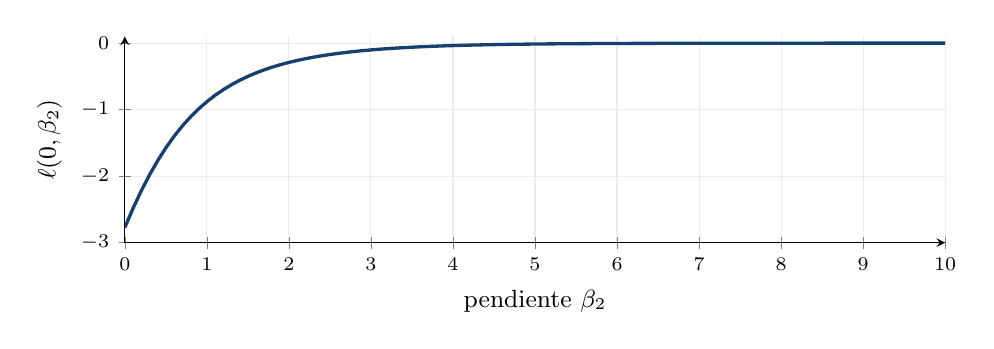
\begin{tikzpicture}
\begin{axis}[base,width=12cm,height=4.2cm,xmin=0,xmax=10,ymin=-3,ymax=.1,xlabel={pendiente $\beta_2$},ylabel={$\ell(0,\beta_2)$}]
\addplot[azul,very thick,domain=0:10]{-2*ln(1+exp(-x))-2*ln(1+exp(-2*x))};
\end{axis}
\end{tikzpicture}
\caption{En los datos separados, aumentar la pendiente mejora la log-verosimilitud, pero no hay máximo finito.}
\end{figure}

\clearpage
\section{Cuasiseparación y observaciones en la frontera}\label{logit37}
La cuasiseparación permite igualdad para algunas filas:
\[
(2y_i-1)\sum_jx_{ij}v_j\ge0\quad\text{para todas},
\]
con al menos una desigualdad estricta y una dirección no nula.
Las filas con margen positivo mejoran al crecer $\beta$ en esa dirección.
Las filas con margen cero no cambian a lo largo de ella.

Para $\beta=\beta^{(0)}+tv$, diferenciar cada contribución respecto de
$t$ permite ver qué sucede sin asumir un límite:
\[
\frac{\dd}{\dd t}\ell(\beta^{(0)}+tv)
=\sum_i
\frac{(2y_i-1)\sum_jx_{ij}v_j}
{1+e^{(2y_i-1)\sum_jx_{ij}(\beta_j^{(0)}+tv_j)}}.
\]
Todos los numeradores son no negativos.
Al menos uno es positivo, y su denominador es finito y positivo
para cualquier $t$ finito.
Por tanto, la derivada total es positiva.
Ningún punto finito en esa trayectoria es un máximo.

\begin{ejemplo}[Dos respuestas opuestas en el mismo valor frontera]
Sean $x_{i2}=(-1,0,0,1)$ y $y=(0,0,1,1)$,
con intercepto cero y dirección $v=(0,1)\T$.
Las filas en $x_{i2}=0$ tienen margen cero y probabilidad $1/2$.
Las filas en $-1$ y $1$ mejoran indefinidamente:
\[
\ell(0,t)=-2\log(1+e^{-t})-2\log2
\longrightarrow-2\log2.
\]
El supremo es menor que cero, pero sigue sin alcanzarse en un punto finito.
\end{ejemplo}
El ejemplo demuestra que respuestas opuestas en un solo patrón
no garantizan ausencia de separación en todas las direcciones.
Es necesario que los patrones que obligan a margen cero cubran
el espacio de parámetros.

Una columna nula es otro fenómeno:
si una dirección produce $\sum_jx_{ij}v_j=0$ para todas las filas,
la log-verosimilitud es exactamente constante, no estrictamente creciente.
Eso es falta de identificación.
Con rango completo, no existe esa dirección nula,
pero todavía pueden existir direcciones cuasiseparadoras.

En el laboratorio original se usarán tres patrones de datos
que aparecen con ambos resultados y cuyas filas son independientes.
Allí cualquier dirección con márgenes no negativos
debe anularse en esos tres patrones y, en consecuencia,
ser la dirección cero. Esa comprobación sí descartará
separación completa y cuasiseparación antes de estimar.

\clearpage
\section{Ausencia de separación y demostración de existencia}\label{logit38}
Supongamos que $X$ tiene rango completo y no existe una dirección
no nula con todos los márgenes $(2y_i-1)x_i\T v$ no negativos.
En cada dirección unitaria debe existir una fila con margen negativo.
Necesitamos demostrar que la pérdida de verosimilitud es uniforme
en todas las direcciones para controlar coeficientes grandes.

La función
\[
v\longmapsto \max_{1\le i\le n}
\left[-(2y_i-1)\sum_jx_{ij}v_j\right]
\]
es continua: es el máximo de un número finito de funciones lineales.
Es estrictamente positiva en la esfera $\norm v_2=1$.
Esa esfera es compacta, por lo que el mínimo se alcanza y es positivo:
\[
\min_{\norm v_2=1}\max_i
\left[-(2y_i-1)\sum_jx_{ij}v_j\right]>0.
\]
Esta cantidad es un número, no una nueva variable de los datos.

Para $\beta=tv$, $t=\norm\beta_2$, alguna fila tiene
$-(2y_i-1)x_i\T v$ al menos tan grande como ese mínimo.
Su contribución cumple
\[
-\log(1+e^{-t(2y_i-1)x_i\T v})
\le -t\min_{\norm u_2=1}\max_i[-(2y_i-1)x_i\T u].
\]
Se usó $\log(1+e^z)\ge z$.
Las demás contribuciones son no positivas.
Por tanto, $\ell(\beta)\to-\infty$ cuando $\norm\beta_2\to\infty$.

La función es continua y, fuera de una bola suficientemente grande,
tiene valores inferiores a $\ell(0)$.
Su máximo global se alcanza dentro de esa bola cerrada y acotada.
La concavidad estricta probada antes demuestra que es único.
Se ha establecido existencia y unicidad mediante dos argumentos diferentes.

\begin{ejemplo}[Los tres patrones mixtos del archivo original]
Las parejas $2,7$ comparten $(1,-1,1)$;
$3,8$ comparten $(1,0,0)$;
$6,11$ comparten $(1,3,1)$.
En cada pareja hay un cero y un uno.
Una dirección de márgenes no negativos exige
\[
v_1-v_2+v_3=0,\quad v_1=0,\quad v_1+3v_2+v_3=0.
\]
Restar la primera ecuación de la tercera da $4v_2=0$.
Luego $v_2=0$, $v_1=0$ y $v_3=0$.
No hay dirección separadora no nula, y esas tres filas son independientes.
\end{ejemplo}
La demostración explica por qué los pares mixtos distribuidos en
direcciones independientes impiden coeficientes infinitos.
Contar solamente cuántos ceros y unos hay en toda la muestra
no realiza esta comprobación geométrica.

\clearpage
\section{El modelo de solo intercepto como solución analítica}\label{logit39}
Si $x_{i1}=1$ y no hay otros regresores,
todas las filas tienen la misma probabilidad
$e^{\beta_1}/(1+e^{\beta_1})$.
La log-verosimilitud queda
\[
\ell(\beta_1)=\beta_1\sum_i y_i-n\log(1+e^{\beta_1}).
\]
Derivar una y dos veces da
\[
\ell'(\beta_1)=\sum_i y_i-\frac{ne^{\beta_1}}{1+e^{\beta_1}},
\qquad
\ell''(\beta_1)=-\frac{ne^{\beta_1}}{(1+e^{\beta_1})^2}.
\]
Si $0<\sum_i y_i<n$, igualar la primera derivada a cero y despejar:
\[
\begin{aligned}
\frac{e^{\widehat\beta_1}}{1+e^{\widehat\beta_1}}
&=\frac{\sum_i y_i}{n},\\
ne^{\widehat\beta_1}
&=(\sum_i y_i)(1+e^{\widehat\beta_1}),\\
(n-\sum_i y_i)e^{\widehat\beta_1}
&=\sum_i y_i,\\
\boxed{\widehat\beta_1}
&=\boxed{\log\frac{\sum_i y_i}{n-\sum_i y_i}}.
\end{aligned}
\]
La ecuación no requiere una nueva letra para el conteo.
Los datos $y_i$ permanecen explícitos.

\begin{ejemplo}[Siete unos y tres ceros]
Con $n=10$, $\sum_i y_i=7$,
$\widehat\beta_1=\log(7/3)\approx.84729786$.
La probabilidad estimada es $7/10$.
La curvatura negativa en el máximo es $-10(.7)(.3)=-2.1$.
Su inversa positiva es $1/2.1$, una escala de varianza asintótica,
no una afirmación exacta de covarianza muestral.
\end{ejemplo}
Cuando $\sum_i y_i=0$, la derivada es negativa en todo punto finito
y el supremo se aproxima con $\beta_1\to-\infty$.
Cuando $\sum_i y_i=n$, es positiva y el coeficiente tiende a $+\infty$.
Estos dos eventos tienen probabilidad positiva para cualquier
probabilidad verdadera estrictamente entre cero y uno.

La solución cerrada permite comprobar un algoritmo iterativo:
cada actualización de Newton puede compararse con el logaritmo exacto.
También permite estudiar sesgo y existencia de momentos en
muestras finitas sin esconder los eventos extremos.
Una fórmula para una normal límite no cambia el comportamiento
de esas configuraciones particulares.

\clearpage
\section{Taylor del gradiente y nacimiento de Newton}\label{logit40}
Buscamos simultáneamente las ecuaciones
$\partial\ell/\partial\beta_l=0$, $l=1,\ldots,k$.
En una iteración $m$, el cambio de coeficientes es
$\Delta^{(m)}=\beta^{(m+1)}-\beta^{(m)}$.
Este vector representa un incremento, no un dato nuevo.

Para una sola coordenada, Taylor da
\[
\frac{\partial\ell(\beta^{(m)}+\Delta)}{\partial\beta_l}
=\frac{\partial\ell(\beta^{(m)})}{\partial\beta_l}
+\sum_{h=1}^k
\frac{\partial^2\ell(\beta^{(m)})}{\partial\beta_l\partial\beta_h}
\Delta_h+O(\norm\Delta_2^2).
\]
El resto es cuadrático porque las segundas derivadas del gradiente
son terceras derivadas de $\ell$, acotadas para datos finitos.
Newton impone cero a la parte lineal:
\[
0=\sum_i x_{il}\left[
y_i-\frac{e^{\sum_jx_{ij}\beta_j^{(m)}}}{1+e^{\sum_jx_{ij}\beta_j^{(m)}}}
\right]
-\sum_{h=1}^k\sum_i
\frac{e^{\sum_jx_{ij}\beta_j^{(m)}}}
{(1+e^{\sum_jx_{ij}\beta_j^{(m)}})^2}
x_{il}x_{ih}\Delta_h^{(m)}.
\]
Mover el segundo término al otro lado construye las $k$ ecuaciones
del sistema de Newton.
La matriz completa suma todos los productos cruzados.

\textbf{Qué se resuelve exactamente.}
El sistema lineal que se acaba de escribir se resuelve con precisión.
Pero es una aproximación de las ecuaciones originales,
porque el resto se ha omitido temporalmente.
Después de actualizar, se recalculan las probabilidades y se
evalúa el gradiente verdadero para medir el error que queda.

\begin{ejemplo}[Un intercepto con diez datos y siete unos]
En $\beta_1^{(0)}=0$, la derivada es $7-10/2=2$
y la segunda es $-10/4=-2.5$.
La ecuación lineal aproximada es $0=2-2.5\Delta_1$,
luego $\Delta_1=.8$ y $\beta_1^{(1)}=.8$.
La raíz exacta es $.84729786$, de modo que aún falta una corrección.
\end{ejemplo}

\begin{figure}[H]\centering
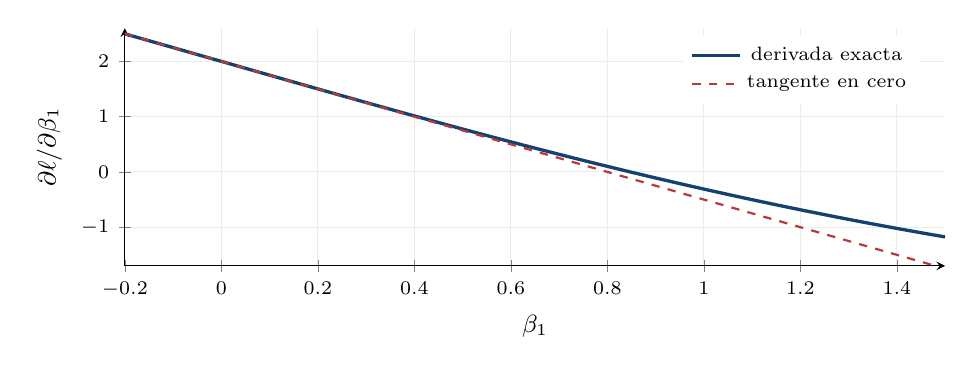
\begin{tikzpicture}
\begin{axis}[base,width=12cm,height=4.6cm,xmin=-.2,xmax=1.5,ymin=-1.7,ymax=2.6,xlabel={$\beta_1$},ylabel={$\partial\ell/\partial\beta_1$},legend pos=north east]
\addplot[azul,very thick,domain=-.2:1.5]{7-10/(1+exp(-x))};\addlegendentry{derivada exacta}\addplot[rojo,dashed,thick,domain=-.2:1.5]{2-2.5*x};\addlegendentry{tangente en cero}
\end{axis}
\end{tikzpicture}
\caption{La tangente al gradiente cruza en $.8$; la raíz de la función exacta está en $\log(7/3)$.}
\end{figure}

\clearpage
\section{La actualización de Newton con todos los datos a la vista}\label{logit41}
Reunir las ecuaciones de Taylor produce el siguiente sistema:
\[
\left[
\sum_i\frac{e^{\sum_jx_{ij}\beta_j^{(m)}}}
{(1+e^{\sum_jx_{ij}\beta_j^{(m)}})^2}x_ix_i\T
\right]\Delta^{(m)}
=
\sum_i x_i\left[
y_i-\frac{e^{\sum_jx_{ij}\beta_j^{(m)}}}
{1+e^{\sum_jx_{ij}\beta_j^{(m)}}}\right].
\]
La matriz tiene $k$ filas y columnas. La columna de ambos lados
tiene $k$ entradas. Si el diseño tiene rango completo,
la matriz es definida positiva en cualquier iteración finita.

La solución matemática es
\[
\boxed{
\begin{aligned}
\beta^{(m+1)}=\beta^{(m)}
&+\left[\sum_i
\frac{e^{\sum_jx_{ij}\beta_j^{(m)}}}
{(1+e^{\sum_jx_{ij}\beta_j^{(m)}})^2}x_ix_i\T\right]^{-1}\\
&\quad\cdot\sum_i x_i\left[
y_i-\frac{e^{\sum_jx_{ij}\beta_j^{(m)}}}
{1+e^{\sum_jx_{ij}\beta_j^{(m)}}}\right].
\end{aligned}}
\]
El signo es positivo porque la Hessiana es el negativo de la
matriz que se está invirtiendo.
No se suma una inversa directamente a los coeficientes:
se suma una columna de correcciones obtenida al multiplicar
la inversa por la columna de derivadas.

\textbf{La corrección de cada coeficiente está acoplada.}
La entrada $l$ del producto usa toda la fila $l$ de la inversa
y todas las derivadas del gradiente.
No basta dividir la derivada de $\beta_l$ por la correspondiente
entrada diagonal de la información. Las entradas cruzadas
afectan al sistema completo.

\begin{ejemplo}[Un sistema pequeño que muestra el acoplamiento]
\[
\begin{pmatrix}2&1\\1&2\end{pmatrix}
\begin{pmatrix}\Delta_1\\\Delta_2\end{pmatrix}
=\begin{pmatrix}1\\0\end{pmatrix}.
\]
La segunda ecuación exige $\Delta_1=-2\Delta_2$.
Sustituir en la primera da $-3\Delta_2=1$:
$\Delta_2=-1/3$, $\Delta_1=2/3$.
Usar solo la diagonal daría $(1/2,0)\T$ y violaría la segunda ecuación.
\end{ejemplo}
La inversa expresa una identidad algebraica.
Para calcularla en dimensión grande, es preferible resolver el
sistema mediante una factorización, porque se evita formar y
redondear una matriz inversa completa.
Las probabilidades y los factores se fijan dentro de esa resolución,
y se recalculan únicamente después de actualizar los coeficientes.

\clearpage
\section{Taylor de la función objetivo y mejora cuadrática predicha}\label{logit42}
El desarrollo de segundo orden de la log-verosimilitud es
\[
\begin{aligned}
\ell(\beta+\Delta)=\ell(\beta)
&+\sum_l\frac{\partial\ell(\beta)}{\partial\beta_l}\Delta_l\\
&+\frac12\sum_l\sum_h
\frac{\partial^2\ell(\beta)}{\partial\beta_l\partial\beta_h}
\Delta_l\Delta_h+O(\norm\Delta_2^3).
\end{aligned}
\]
Al sustituir las derivadas, la parte variable de la aproximación es
\[
\begin{aligned}
&\sum_i\left[y_i-
\frac{e^{\sum_jx_{ij}\beta_j}}{1+e^{\sum_jx_{ij}\beta_j}}\right]
\left(\sum_lx_{il}\Delta_l\right)\\
&\quad-\frac12\sum_i
\frac{e^{\sum_jx_{ij}\beta_j}}{(1+e^{\sum_jx_{ij}\beta_j})^2}
\left(\sum_lx_{il}\Delta_l\right)^2.
\end{aligned}
\]
El primer término es lineal en el incremento; el segundo es cuadrático
y no positivo. En esta aproximación los datos y todas las fracciones
se evalúan en el $\beta$ actual y se consideran fijos al elegir $\Delta$.

Derivar esta expresión respecto de $\Delta_h$ da
\[
\sum_i x_{ih}\left[y_i-
\frac{e^{\sum_jx_{ij}\beta_j}}{1+e^{\sum_jx_{ij}\beta_j}}\right]
-\sum_i
\frac{e^{\sum_jx_{ij}\beta_j}}{(1+e^{\sum_jx_{ij}\beta_j})^2}
x_{ih}\sum_lx_{il}\Delta_l.
\]
Igualar todas estas derivadas a cero reproduce el sistema de Newton.
Así, resolver una tangente del gradiente y maximizar una aproximación
cuadrática de la función son dos deducciones de la misma corrección.

En la solución del sistema, multiplicar por $\Delta\T$ muestra
que el término lineal coincide con la forma cuadrática positiva.
Por tanto, la mejora predicha es
\[
\frac12\sum_i
\frac{e^{\sum_jx_{ij}\beta_j}}{(1+e^{\sum_jx_{ij}\beta_j})^2}
\left(\sum_lx_{il}\Delta_l\right)^2>0
\]
si el gradiente es no nulo y el diseño tiene rango completo.

\begin{ejemplo}[Un intercepto y el primer paso]
Con diez datos y siete unos, en cero el incremento es $.8$.
La mejora cuadrática predicha es
$2(.8)-\tfrac12(2.5)(.8)^2=.8$.
La mejora exacta se calcula con la log-verosimilitud logística,
y no tiene que ser exactamente $.8$.
\end{ejemplo}
El resto de tercer orden explica la diferencia.
Lejos del máximo, un incremento grande puede hacer que la
aproximación deje de describir bien a la función real.
Un método amortiguado comprobará la mejora real antes de aceptar
el paso completo.

\clearpage
\section{Eliminación: resolver las tres correcciones sin abreviar la matriz}\label{logit43}
En el inicio de los doce datos, el sistema es
\[
\begin{pmatrix}3&3&7/4\\3&25/2&7/4\\7/4&7/4&9/4\end{pmatrix}
\begin{pmatrix}\Delta_1\\\Delta_2\\\Delta_3\end{pmatrix}
=\begin{pmatrix}1\\5\\1/2\end{pmatrix}.
\]
Abrimos las tres ecuaciones:
\[
\begin{aligned}
3\Delta_1+3\Delta_2+(7/4)\Delta_3&=1,\\
3\Delta_1+(25/2)\Delta_2+(7/4)\Delta_3&=5,\\
(7/4)\Delta_1+(7/4)\Delta_2+(9/4)\Delta_3&=1/2.
\end{aligned}
\]
Restar la primera a la segunda conserva la solución
porque se resta la misma igualdad en ambos miembros.
Los términos en $\Delta_1$ y $\Delta_3$ se cancelan:
\[
(25/2-3)\Delta_2=5-1,\quad
(19/2)\Delta_2=4,\quad \boxed{\Delta_2=8/19}.
\]
Restar $7/12$ veces la primera a la tercera cancela simultáneamente
los primeros dos términos:
\[
\left(9/4-\frac7{12}\frac74\right)\Delta_3
=\frac12-\frac7{12}.
\]
La cuenta de ambos lados, con el mismo denominador, es
\[
\frac{108-49}{48}\Delta_3=\frac{6-7}{12},
\quad \frac{59}{48}\Delta_3=-\frac1{12},
\quad \boxed{\Delta_3=-4/59}.
\]
Volver a la primera ecuación despeja el intercepto:
\[
\begin{aligned}
\Delta_1
&=\frac{1-3(8/19)-(7/4)(-4/59)}3\\
&=\frac{1-24/19+7/59}3
=\frac{1121-1416+133}{3363}
=\boxed{-54/1121}.
\end{aligned}
\]
No se usaron letras para esconder las seis entradas distintas
de la matriz. Cada operación se puede verificar con las cifras originales.

Como el inicio era $\beta^{(0)}=0$, el nuevo vector coincide con
la corrección:
\[
\beta^{(1)}=
\begin{pmatrix}-54/1121\\8/19\\-4/59\end{pmatrix}.
\]
En iteraciones posteriores hay que sumar la corrección al vector actual.
Copiarla directamente como estimación produciría otro algoritmo.

Los pivotes son $3$, $19/2$ y $59/48$.
Su producto es $1121/32$, el determinante de la matriz del sistema.
Son positivos, coherentemente con su positividad definida.
Una resolución numérica usa este tipo de eliminación con controles
de precisión; el desarrollo con fracciones muestra la misma operación
sin errores intermedios de redondeo.

\clearpage
\section{Cholesky: construir y verificar el factor triangular}\label{logit44}
Una matriz definida positiva puede escribirse como $LL\T$,
con $L$ triangular inferior de diagonal positiva.
$L$ es un factor de la matriz, no un cambio de nombre
de la matriz de información.
Para tres coeficientes, multiplicar sus entradas da
\[
\begin{pmatrix}l_{11}&0&0\\l_{21}&l_{22}&0\\l_{31}&l_{32}&l_{33}\end{pmatrix}
\begin{pmatrix}l_{11}&l_{21}&l_{31}\\0&l_{22}&l_{32}\\0&0&l_{33}\end{pmatrix}
=
\begin{pmatrix}
l_{11}^2&l_{11}l_{21}&l_{11}l_{31}\\
l_{11}l_{21}&l_{21}^2+l_{22}^2&l_{21}l_{31}+l_{22}l_{32}\\
l_{11}l_{31}&l_{21}l_{31}+l_{22}l_{32}&l_{31}^2+l_{32}^2+l_{33}^2
\end{pmatrix}.
\]
Igualar con la matriz inicial del laboratorio permite despejar
una entrada cada vez:
\[
\begin{aligned}
l_{11}^2=3&\Rightarrow l_{11}=\sqrt3,\\
l_{11}l_{21}=3&\Rightarrow l_{21}=\sqrt3,\\
l_{11}l_{31}=7/4&\Rightarrow l_{31}=7/(4\sqrt3),\\
l_{21}^2+l_{22}^2=25/2&\Rightarrow l_{22}=\sqrt{19/2},\\
l_{21}l_{31}+l_{22}l_{32}=7/4&\Rightarrow l_{32}=0,\\
l_{31}^2+l_{32}^2+l_{33}^2=9/4&\Rightarrow l_{33}=\sqrt{59/48}.
\end{aligned}
\]
Se eligieron las raíces positivas en la diagonal.
El factor es
\[
L=\begin{pmatrix}
\sqrt3&0&0\\
\sqrt3&\sqrt{19/2}&0\\
7/(4\sqrt3)&0&\sqrt{59/48}
\end{pmatrix}.
\]
Multiplicarlo por su transpuesta comprueba cada entrada.
Por ejemplo, la última diagonal es $49/48+59/48=108/48=9/4$.

Resolver $LL\T\Delta=(1,5,1/2)\T$ se hace en dos sustituciones.
Primero se determinan las tres entradas de $L\T\Delta$:
\[
(L\T\Delta)_1=1/\sqrt3,\quad
(L\T\Delta)_2=4/\sqrt{19/2},\quad
(L\T\Delta)_3=-1/(12\sqrt{59/48}).
\]
Después se resuelve el sistema triangular superior desde la
última fila a la primera:
\[
\Delta_3=\frac{-1}{12(59/48)}=-4/59,\qquad
\Delta_2=\frac4{19/2}=8/19,
\]
\[
\Delta_1=\frac{1/\sqrt3-\sqrt3(8/19)
-\{7/(4\sqrt3)\}(-4/59)}{\sqrt3}=-54/1121.
\]
Las dos etapas mantienen toda la matriz y sus términos cruzados.
Coinciden con la eliminación anterior y evitan formar una inversa completa.

\clearpage
\section{Ascenso, amortiguación y búsqueda de paso}\label{logit45}
Sea $\Delta$ la corrección obtenida por el sistema de Newton.
Multiplicar ese sistema por $\Delta\T$ da
\[
\nabla_\beta\ell(\beta)\T\Delta
=\sum_i
\frac{e^{\sum_jx_{ij}\beta_j}}{(1+e^{\sum_jx_{ij}\beta_j})^2}
\left(\sum_jx_{ij}\Delta_j\right)^2>0
\]
cuando el gradiente no es cero y el diseño tiene rango completo.
La derivada de $\ell(\beta+\alpha\Delta)$ respecto de $\alpha$
en cero es exactamente ese número positivo.
Por continuidad, existe un paso positivo suficientemente pequeño
que aumenta la log-verosimilitud.

No se ha demostrado que $\alpha=1$ la aumente.
La función a lo largo de la trayectoria puede dejar atrás el máximo
local de esa recta antes de llegar al final del paso completo.
Un método amortiguado usa
\[
\beta^{(m+1)}=\beta^{(m)}+\alpha_m\Delta^{(m)},\qquad 0<\alpha_m\le1.
\]
Una regla de aceptación pide
\[
\ell(\beta+\alpha\Delta)\ge
\ell(\beta)+c\alpha\,\nabla_\beta\ell(\beta)\T\Delta,
\qquad 0<c<1.
\]
El número $c$ controla la mejora mínima exigida.
Se prueba primero $\alpha=1$ y, si no cumple, se reduce
por un factor fijo, por ejemplo $1/2$.
La derivada positiva en cero garantiza aceptación de un paso
suficientemente pequeño.

\begin{ejemplo}[Un intercepto que muestra el fallo del paso completo]
Con diez datos y siete unos, si se comienza en $\beta_1=-5$,
la probabilidad es muy pequeña y la curvatura también:
\[
\Delta_1=
\frac{7-10/(1+e^5)}{10e^{-5}/(1+e^{-5})^2}.
\]
El incremento supera $100$ y el nuevo coeficiente supera $95$.
La log-verosimilitud en ese punto es inferior a $-285$,
mientras que al comenzar es aproximadamente $-35.067$.
La dirección es de ascenso local, pero el paso completo es excesivo.
\end{ejemplo}
Una evaluación estable de la log-verosimilitud es esencial durante
esta búsqueda: un desbordamiento aritmético podría confundirse con
una función mal comportada.
La aceptación se verifica con la función exacta y no solamente con
la mejora predicha por Taylor.

Amortiguar controla el tamaño de pasos, pero no elimina separación.
Si no existe un máximo finito, una secuencia de pasos aceptados puede
seguir empujando coeficientes hacia el infinito.
La geometría de los datos debe comprobarse por separado.

\clearpage
\section{Convergencia cuadrática local con el resto de Taylor controlado}\label{logit46}
Supongamos que existe un máximo finito $\widehat\beta$ y que la Hessiana
es invertible en una vecindad de él.
Usamos la versión integral de Taylor para el gradiente:
\[
\nabla_\beta\ell(\beta)-\nabla_\beta\ell(\widehat\beta)
=\int_0^1\nabla_\beta^2\ell(
\widehat\beta+t(\beta-\widehat\beta))\dd t\,
(\beta-\widehat\beta).
\]
El gradiente del máximo es cero.
La integral no se reemplaza por una Hessiana en un único punto
sin demostrarlo: esa forma escalar del valor medio no se extiende
automáticamente a todas las coordenadas de un vector.

El paso completo de Newton es
$\beta^{\mathrm{nueva}}=\beta-
[\nabla_\beta^2\ell(\beta)]^{-1}\nabla_\beta\ell(\beta)$.
Restar $\widehat\beta$ y sustituir la integral:
\[
\begin{aligned}
\beta^{\mathrm{nueva}}-\widehat\beta
={}&[\nabla_\beta^2\ell(\beta)]^{-1}
\int_0^1\Big[
\nabla_\beta^2\ell(\beta)\\
&-\nabla_\beta^2\ell(
\widehat\beta+t(\beta-\widehat\beta))
\Big]\dd t\,(\beta-\widehat\beta).
\end{aligned}
\]
Las terceras derivadas acotadas hacen que la diferencia entre
Hessianas esté acotada por una constante por la distancia entre
sus argumentos.
La distancia del argumento intermedio a $\beta$ es
$(1-t)\norm{\beta-\widehat\beta}_2$.
Si la norma de la inversa de Hessiana está acotada en la vecindad,
\[
\norm{\beta^{\mathrm{nueva}}-\widehat\beta}_2
\le C\norm{\beta-\widehat\beta}_2^2\int_0^1(1-t)\dd t
=\frac C2\norm{\beta-\widehat\beta}_2^2.
\]
Esta es la convergencia cuadrática local: el error siguiente es
de orden del cuadrado del error actual.

\begin{ejemplo}[Qué significa cuadrática]
Si la constante efectiva fuera dos y el error actual $.01$,
la cota del siguiente sería $2(.01)^2=.0002$.
Aplicarla de nuevo daría $2(.0002)^2=.00000008$.
La aceleración requiere haber entrado en la vecindad adecuada.
\end{ejemplo}
La demostración usa existencia, invertibilidad y control local
de las derivadas.
No afirma convergencia desde cualquier inicio ni en datos separados.
Los números finales del laboratorio mostrarán la reducción rápida
del gradiente una vez que el algoritmo se acerque al máximo.

Un factor pequeño de varianza Bernoulli puede volver grande la
norma de la inversa. Entonces la vecindad donde la cota es útil
puede ser reducida.
Por eso se combinan comprobaciones de rango, búsqueda de paso
y evaluación de curvatura.

\clearpage
\section{IRLS: la respuesta de trabajo escrita sin una letra sustituta}\label{logit47}
La aproximación local de la media puede invertirse para construir una
respuesta de trabajo que vive en la escala del producto lineal.
Para una iteración fija, su valor en la fila $i$ es
\[
\sum_jx_{ij}\beta_j^{(m)}
+
\frac{
y_i-\dfrac{e^{\sum_jx_{ij}\beta_j^{(m)}}}
{1+e^{\sum_jx_{ij}\beta_j^{(m)}}}}
{\dfrac{e^{\sum_jx_{ij}\beta_j^{(m)}}}
{(1+e^{\sum_jx_{ij}\beta_j^{(m)}})^2}}.
\]
Se muestra completa la expresión en vez de rebautizarla.
El primer término es el valor lineal actual.
El segundo divide la discrepancia en respuesta por la pendiente
de la función logística respecto de ese valor lineal.

Esta construcción proviene de aproximar
$Y_i\approx\Prob(Y_i=1\mid x_i)+
\frac{\partial\Prob(Y_i=1\mid x_i)}{\partial(x_i\T\beta)}
\{x_i\T\beta^{\mathrm{nueva}}-x_i\T\beta^{(m)}\}$.
Despejar el producto lineal nuevo produce la expresión anterior.
Es una inversión de la tangente, no una transformación exacta
de una respuesta binaria aleatoria.

\begin{ejemplo}[Trabajar desde coeficientes cero]
En cero, el producto lineal es cero, la probabilidad es $1/2$ y
su derivada es $1/4$.
La respuesta de trabajo es
\[
0+\frac{y_i-1/2}{1/4}=4y_i-2=
\begin{cases}-2,&y_i=0,\\2,&y_i=1.\end{cases}
\]
Los valores $-2$ y $2$ no son probabilidades.
Su escala es la del producto lineal de los coeficientes.
\end{ejemplo}
El peso de mínimos cuadrados en la misma fila es
\[
\frac{e^{\sum_jx_{ij}\beta_j^{(m)}}}
{(1+e^{\sum_jx_{ij}\beta_j^{(m)}})^2}.
\]
Multiplicar la respuesta de trabajo por ese peso cancela el
denominador de la segunda parte:
\[
\frac{e^{\sum_jx_{ij}\beta_j^{(m)}}}
{(1+e^{\sum_jx_{ij}\beta_j^{(m)}})^2}
\sum_jx_{ij}\beta_j^{(m)}
+y_i-\frac{e^{\sum_jx_{ij}\beta_j^{(m)}}}
{1+e^{\sum_jx_{ij}\beta_j^{(m)}}}.
\]
Esta cancelación es el puente exacto entre el sistema ponderado
y el sistema de Newton.

Cuando la probabilidad está muy cerca de cero o uno,
el denominador de la respuesta de trabajo es pequeño.
Su valor puede ser grande. Eso no demuestra por sí solo
un dato atípico en la respuesta original.
Es una propiedad de invertir una tangente con poca pendiente.
En cómputo se puede resolver el sistema de Newton sin construir
explícitamente una respuesta de trabajo enorme.

\clearpage
\section{Derivar mínimos cuadrados ponderados y recuperar Newton}\label{logit48}
En una iteración, los factores actuales se mantienen fijos
al elegir el nuevo vector de coeficientes.
La función ponderada que se minimiza es
\[
\begin{aligned}
\sum_i
\frac{e^{\sum_jx_{ij}\beta_j^{(m)}}}
{(1+e^{\sum_jx_{ij}\beta_j^{(m)}})^2}
\bigg[&
\sum_jx_{ij}\beta_j^{(m)}
+\frac{y_i-\dfrac{e^{\sum_jx_{ij}\beta_j^{(m)}}}
{1+e^{\sum_jx_{ij}\beta_j^{(m)}}}}
{\dfrac{e^{\sum_jx_{ij}\beta_j^{(m)}}}
{(1+e^{\sum_jx_{ij}\beta_j^{(m)}})^2}}\\
&-\sum_jx_{ij}\beta_j^{\mathrm{nueva}}\bigg]^2.
\end{aligned}
\]
Diferenciar respecto de $\beta_l^{\mathrm{nueva}}$ multiplica
cada corchete por $-2x_{il}$ y por su peso.
Igualar a cero, cancelar $-2$ y multiplicar la respuesta de
trabajo por el peso da
\[
\begin{aligned}
\sum_i
\frac{e^{\sum_jx_{ij}\beta_j^{(m)}}}
{(1+e^{\sum_jx_{ij}\beta_j^{(m)}})^2}
x_{il}\sum_jx_{ij}\beta_j^{\mathrm{nueva}}
={}&\sum_i
\frac{e^{\sum_jx_{ij}\beta_j^{(m)}}}
{(1+e^{\sum_jx_{ij}\beta_j^{(m)}})^2}
x_{il}\sum_jx_{ij}\beta_j^{(m)}\\
&+\sum_i x_{il}\left[y_i-
\frac{e^{\sum_jx_{ij}\beta_j^{(m)}}}
{1+e^{\sum_jx_{ij}\beta_j^{(m)}}}\right].
\end{aligned}
\]
Restar el primer término del lado derecho deja
\[
\sum_i
\frac{e^{\sum_jx_{ij}\beta_j^{(m)}}}
{(1+e^{\sum_jx_{ij}\beta_j^{(m)}})^2}
x_{il}\sum_jx_{ij}
(\beta_j^{\mathrm{nueva}}-\beta_j^{(m)})
=\sum_i x_{il}\left[y_i-
\frac{e^{\sum_jx_{ij}\beta_j^{(m)}}}
{1+e^{\sum_jx_{ij}\beta_j^{(m)}}}\right].
\]
Esta es la ecuación de Newton para la coordenada $l$,
con incremento $\beta^{\mathrm{nueva}}-\beta^{(m)}$.
No se ha usado una equivalencia aproximada en este paso algebraico:
una vez fijadas las respuestas de trabajo y los pesos,
ambos sistemas son exactamente el mismo.

La Hessiana del objetivo ponderado respecto del nuevo coeficiente
es dos veces la matriz positiva del sistema de Newton.
Por eso su mínimo es único si el diseño tiene rango completo.
IRLS se llama iterativo porque las fracciones se recalculan
después de obtener el nuevo vector.

La suma de cuadrados local no es la log-verosimilitud global.
Al cambiar los coeficientes cambian las respuestas de trabajo.
La igualdad entre sus sistemas no autoriza a aplicar
automáticamente las varianzas exactas de una regresión lineal
con errores normales a un modelo Bernoulli.

\clearpage
\section{Evaluación estable de la logística y de la log-verosimilitud}\label{logit49}
Una identidad válida puede evaluarse mal con aritmética finita.
Si el producto $\sum_jx_{ij}\beta_j$ es grande, calcular su exponencial
directamente puede desbordar.
Usamos expresiones equivalentes según su signo:
\[
\Prob(Y_i=1\mid x_i)=
\begin{cases}
\dfrac1{1+e^{-\sum_jx_{ij}\beta_j}},
&\sum_jx_{ij}\beta_j\ge0,\\[6pt]
\dfrac{e^{\sum_jx_{ij}\beta_j}}
{1+e^{\sum_jx_{ij}\beta_j}},
&\sum_jx_{ij}\beta_j<0.
\end{cases}
\]
En la primera rama el exponente es no positivo.
En la segunda también lo es.
Así se evita una exponencial enorme para calcular una
probabilidad que debe estar entre cero y uno.

Para el término logarítmico,
\[
\log(1+e^{\sum_jx_{ij}\beta_j})
=\max(0,\sum_jx_{ij}\beta_j)
+\log(1+e^{-|\sum_jx_{ij}\beta_j|}).
\]
Si el producto es positivo, se factoriza su exponencial.
Si es negativo, la identidad conserva la fórmula original.
En ambos casos la última exponencial no supera uno.

\textbf{Calcular una fila sin restar números enormes.}
Una forma estable de la contribución Bernoulli es
\[
-\max(0,-(2y_i-1)\sum_jx_{ij}\beta_j)
-\log\left(1+e^{-|\sum_jx_{ij}\beta_j|}\right).
\]
Para $y_i=1$ y un producto positivo grande,
queda un número cercano a cero sin restar ese producto
de otro número casi idéntico.
Para un resultado mal predicho, la contribución permanece
grande en valor absoluto, como exige la función exacta.

\begin{ejemplo}[Un producto lineal de mil]
Si $\sum_jx_{ij}\beta_j=1000$ y $y_i=1$,
la contribución es $-\log(1+e^{-1000})$, prácticamente cero.
Si $y_i=0$, es $-1000-\log(1+e^{-1000})$,
prácticamente $-1000$.
No se necesita calcular $e^{1000}$.
\end{ejemplo}
Redondear una probabilidad a uno en pantalla no demuestra
que matemáticamente sea uno.
La curvatura puede ser muy pequeña y el inversor puede volverse
inestable antes de que el modelo alcance un extremo exacto.

Una implementación debe controlar residuos del sistema,
simetría numérica de la matriz y tamaño de las correcciones.
Pero esos controles computacionales no reemplazan la
comprobación estadística de existencia e identificación.
El programa y la matemática deben examinarse de forma coherente.

\clearpage
\section{Criterios de parada y señales de falsa convergencia}\label{logit50}
Hay al menos tres cantidades diferentes que medir:
la norma del gradiente, el tamaño del incremento y el cambio
de log-verosimilitud.
El gradiente en un punto se calcula con las probabilidades
de ese mismo punto:
\[
\max_l\left|
\sum_i x_{il}\left[
y_i-\frac{e^{\sum_jx_{ij}\beta_j}}{1+e^{\sum_jx_{ij}\beta_j}}
\right]\right|.
\]
Si es pequeño, las condiciones de primer orden se satisfacen
aproximadamente. El resultado depende de las unidades de los
regresores: una columna reescalada cambia su componente de gradiente.

El tamaño del incremento puede medirse relativamente:
\[
\frac{\norm{\beta^{(m+1)}-\beta^{(m)}}_2}
{1+\norm{\beta^{(m)}}_2}.
\]
La constante uno evita dividir por cero al comenzar.
Un paso pequeño puede deberse a un máximo cercano, pero también
a una búsqueda de paso excesivamente amortiguada.

La variación de función usa
\[
\frac{|\ell(\beta^{(m+1)})-\ell(\beta^{(m)})|}
{1+|\ell(\beta^{(m)})|}.
\]
Una variación pequeña es compatible con una asíntota plana.
En separación, la log-verosimilitud puede acercarse a su supremo
mientras los coeficientes siguen creciendo.

\begin{ejemplo}[Todos los resultados son uno]
En un modelo de intercepto con $y_i=1$ para todas las filas,
\[
\ell(\beta_1)=-n\log(1+e^{-\beta_1}),\quad
\ell'(\beta_1)=\frac n{1+e^{\beta_1}}.
\]
Ambas cantidades se aproximan a cero cuando $\beta_1\to+\infty$.
Eso no significa que exista una raíz finita de la derivada.
\end{ejemplo}
Por eso los tres controles se combinan con observación de
crecimiento de coeficientes y pérdida de curvatura.
En una muestra de rango completo y sin separación, una
solución de gradiente casi nulo con matriz positiva estable
tiene una interpretación diferente de una secuencia que se
aleja indefinidamente.

La tolerancia de optimización no es un nivel de significancia.
Una tolerancia de $10^{-10}$ indica precisión al resolver
ecuaciones, no una probabilidad de error estadístico.
Los intervalos de confianza dependen de distribución muestral
y no del número de decimales mostrado por el algoritmo.

Las cuentas numéricas del tratado se calculan con mayor precisión
que la que aparece en las tablas.
Volver a sumar únicamente los decimales impresos puede producir
una pequeña diferencia, atribuible al redondeo y no al modelo.

\clearpage
\section{La log-verosimilitud esperada y la desigualdad que identifica al parámetro}\label{logit51}
Supongamos que el modelo verdadero tiene coeficientes $\beta_\star$.
Para cada fila, la esperanza de la contribución del candidato $\beta$ es
\[
\frac{e^{\sum_jx_{ij}\beta_{\star j}}}
{1+e^{\sum_jx_{ij}\beta_{\star j}}}
\log\frac{e^{\sum_jx_{ij}\beta_j}}
{1+e^{\sum_jx_{ij}\beta_j}}
+
\frac1{1+e^{\sum_jx_{ij}\beta_{\star j}}}
\log\frac1{1+e^{\sum_jx_{ij}\beta_j}}.
\]
Restar su valor en el parámetro verdadero produce el negativo
de una divergencia entre dos distribuciones Bernoulli.

Para demostrar su signo, consideremos las dos posibilidades $y_i=0,1$
y usemos $\log u\le u-1$ para $u>0$.
Esta desigualdad se obtiene porque
$u-1-\log u$ tiene derivada $1-1/u$, mínimo en uno y valor cero allí.
Entonces
\[
\begin{aligned}
&\sum_{y_i=0}^1
\Prob_{\beta_\star}(Y_i=y_i\mid x_i)
\log\frac{\Prob_\beta(Y_i=y_i\mid x_i)}
{\Prob_{\beta_\star}(Y_i=y_i\mid x_i)}\\
&\le\sum_{y_i=0}^1
\left[\Prob_\beta(Y_i=y_i\mid x_i)
-\Prob_{\beta_\star}(Y_i=y_i\mid x_i)\right]=0.
\end{aligned}
\]
La igualdad requiere que las dos masas candidatas coincidan
con las verdaderas. Bajo identificación, esto fuerza el
mismo vector de coeficientes.

Agregar todas las filas demuestra que la log-verosimilitud
esperada es máxima en $\beta_\star$.
Se trata de una afirmación sobre una función promediada,
no sobre el máximo de una muestra particular.
Las fluctuaciones de $Y_i$ hacen que el máximo observado
esté en otro punto.

\begin{ejemplo}[Penalizar una probabilidad falsa]
Si la probabilidad verdadera del uno es $.8$ y se propone $.5$,
la diferencia esperada por fila es
\[
.8\log(.5/.8)+.2\log(.5/.2)\approx-.192745.
\]
Proponer la distribución verdadera da diferencia cero.
\end{ejemplo}
Para probar consistencia hace falta además que los promedios
muestrales se acerquen uniformemente a estas esperanzas y
que el máximo estimado permanezca en una región controlada.
La desigualdad demuestra cuál es el objetivo poblacional;
no demuestra por sí sola toda la convergencia del estimador.

Bajo especificación incorrecta, el máximo esperado elige
la distribución logística más cercana según esta pérdida,
que puede ser un parámetro de aproximación.
No se interpreta automáticamente como el parámetro de
una ecuación causal.

\clearpage
\section{Consistencia: controlar uniformemente el promedio de log-verosimilitudes}\label{logit52}
Para una demostración concreta supongamos datos iid,
regresores acotados y un conjunto compacto de coeficientes que contiene
al parámetro verdadero en su interior.
Estas hipótesis facilitan una prueba completa; otras formulaciones
requieren condiciones de momentos y control de colas.

La contribución individual tiene gradiente
\[
x_i\left[y_i-\frac{e^{\sum_jx_{ij}\beta_j}}
{1+e^{\sum_jx_{ij}\beta_j}}\right].
\]
El valor absoluto de la diferencia es como máximo uno.
Si $\norm{x_i}_2\le M$, la norma de ese gradiente es como máximo $M$.
Integrar la derivada a lo largo de un segmento produce
\[
\left|
\left[y_i\sum_jx_{ij}\beta_j-\log(1+e^{\sum_jx_{ij}\beta_j})\right]
-
\left[y_i\sum_jx_{ij}\widetilde\beta_j
-\log(1+e^{\sum_jx_{ij}\widetilde\beta_j})\right]
\right|\le M\norm{\beta-\widetilde\beta}_2.
\]
El promedio muestral conserva esta misma cota.
La esperanza de la contribución también la conserva.

Por compacidad, para cada $\delta>0$ se puede cubrir el espacio
de coeficientes con un número finito de bolas de radio $\delta$.
En el centro de cada bola, la ley de grandes números hace que el
promedio de contribuciones converja a su esperanza.
Como hay un número finito de centros, el máximo de esos errores
también converge a cero: la probabilidad de que alguno exceda
una tolerancia se acota por la suma de esas probabilidades.

Para cualquier coeficiente dentro de una bola, la diferencia
entre su error y el del centro está acotada por $2M\delta$:
un $M\delta$ para el promedio y otro para la esperanza.
Por tanto,
\[
\sup_\beta\left|
\frac{\ell(\beta;Y,X)}n-
\E\!\left[Y_i\sum_jx_{ij}\beta_j-
\log(1+e^{\sum_jx_{ij}\beta_j})\right]
\right|
\le \max_{\text{centros}}|\text{error en el centro}|+2M\delta.
\]
Primero se toma $n$ grande y después $\delta$ pequeño.
Esto demuestra convergencia uniforme en probabilidad.

La ley de grandes números en un punto no bastaría para controlar
un máximo que cambia de lugar con la muestra.
La cobertura finita y la cota de derivadas son los pasos que
permiten pasar del control puntual al uniforme.
No se ha supuesto que los coeficientes observados ya sean
iguales a los verdaderos.

\clearpage
\section{Consistencia: separar el máximo verdadero de los demás parámetros}\label{logit53}
La desigualdad de divergencia demostró que la esperanza de la
log-verosimilitud por fila es máxima en el parámetro verdadero.
Supongamos identificación y las condiciones de convergencia
uniforme desarrolladas en la unidad anterior.

Para una tolerancia $\varepsilon>0$, consideremos todos los
coeficientes del conjunto compacto cuya distancia a $\beta_\star$
es al menos $\varepsilon$.
Ese conjunto es cerrado y compacto.
La función esperada es continua y su máximo en ese conjunto se
alcanza. Por identificación, su valor es estrictamente menor
que el valor en $\beta_\star$.

Por tanto existe una brecha positiva entre el valor esperado
verdadero y el mayor valor esperado fuera de la bola:
\[
\begin{aligned}
&\E\!\left[Y_i\sum_jx_{ij}\beta_{\star j}
-\log(1+e^{\sum_jx_{ij}\beta_{\star j}})\right]\\
&\quad-\sup_{\norm{\beta-\beta_\star}_2\ge\varepsilon}
\E\!\left[Y_i\sum_jx_{ij}\beta_j
-\log(1+e^{\sum_jx_{ij}\beta_j})\right]>0.
\end{aligned}
\]

Si el error uniforme del promedio es menor que un tercio de esa
brecha, para cualquier coeficiente fuera de la bola,
su promedio muestral es menor que el promedio en $\beta_\star$.
La cuenta suma dos errores como máximo, que no alcanzan
a cerrar la brecha poblacional.
Un maximizador muestral no puede estar fuera de la bola.

La probabilidad de que el error uniforme exceda esa cantidad
tiende a cero. Luego
\[
\Prob(\norm{\widehat\beta-\beta_\star}_2\ge\varepsilon)\longrightarrow0.
\]
Eso es consistencia: el estimador se acerca al parámetro en
probabilidad cuando crece la muestra.

\begin{cuidado}[La restricción compacta y el máximo sin restricciones]
La prueba anterior garantiza existencia de un máximo en el
conjunto compacto incluso si una muestra está separada.
Para el máximo sin restricciones se necesita demostrar además
que permanece en una región controlada y que la probabilidad
de problemas de existencia tiende a cero.
No se elimina una hipótesis técnica sin reemplazar su función.
\end{cuidado}
Si el verdadero parámetro está en el interior del conjunto
compacto, la consistencia implica que con probabilidad creciente
el máximo estimado es interior.
Allí puede usarse la ecuación de gradiente cero y desarrollar
la aproximación normal.

Si el modelo está mal especificado, la misma prueba puede
converger al máximo esperado de aproximación, en vez de a un
parámetro verdadero del enlace logístico.
La convergencia de un algoritmo y la consistencia estadística
son conceptos diferentes: uno repite iteraciones en una muestra,
el otro compara muestras de tamaño creciente.

\clearpage
\section{Normalidad del gradiente: construir el límite desde sus momentos}\label{logit54}
En el parámetro verdadero, la contribución de una fila al gradiente es
\[
x_i\left[
Y_i-\frac{e^{\sum_jx_{ij}\beta_{\star j}}}
{1+e^{\sum_jx_{ij}\beta_{\star j}}}\right].
\]
Su esperanza es cero.
Con datos iid y segundo momento finito, sus sumas normalizadas
satisfacen un teorema central del límite vectorial.

Para ver su origen, proyectemos sobre una dirección fija $v$.
La contribución escalar es
\[
\left(\sum_jx_{ij}v_j\right)
\left[
Y_i-\frac{e^{\sum_jx_{ij}\beta_{\star j}}}
{1+e^{\sum_jx_{ij}\beta_{\star j}}}\right].
\]
Su varianza se calcula condicionando en $x_i$:
\[
\E\!\left[
\frac{e^{\sum_jx_{ij}\beta_{\star j}}}
{(1+e^{\sum_jx_{ij}\beta_{\star j}})^2}
\left(\sum_jx_{ij}v_j\right)^2\right].
\]
La independencia entre filas hace aditiva esa varianza.

La función característica de una variable centrada de varianza
finita tiene expansión
$1-\tfrac12t^2\Var+o(t^2)$ cerca de cero.
La característica de la suma dividida por $\sqrt n$
es la potencia $n$ de esa expresión evaluada en $t/\sqrt n$.
Su límite es $\exp(-t^2\Var/2)$, la característica de una normal.
Hacerlo para todas las direcciones $v$ produce el límite vectorial:
\[
\frac1{\sqrt n}\nabla_\beta\ell(\beta_\star;Y,X)
\ \xrightarrow{\mathrm d}\
\mathcal N_k\!\left(
0,\
\E\!\left[
\frac{e^{\sum_jx_{ij}\beta_{\star j}}}
{(1+e^{\sum_jx_{ij}\beta_{\star j}})^2}x_ix_i\T
\right]\right).
\]
La matriz dentro de la normal conserva todas las covarianzas
entre coordenadas del gradiente.

\begin{ejemplo}[Una covarianza fuera de la diagonal]
Si $k=2$, las coordenadas son intercepto y una pendiente.
La entrada $(1,2)$ de la matriz límite es
\[
\E\!\left[
\frac{e^{\beta_{\star1}+x_{i2}\beta_{\star2}}}
{(1+e^{\beta_{\star1}+x_{i2}\beta_{\star2}})^2}x_{i2}\right].
\]
Puede no ser cero, incluso si se centró la variable sin usar
los mismos factores de ponderación.
\end{ejemplo}
La normalidad del límite no significa que la suma finita de
Bernoulli sea exactamente normal.
Con tamaño de muestra pequeño o información casi singular,
la aproximación puede ser deficiente.
La siguiente unidad aplicará este límite a la expansión
de las ecuaciones que definen al estimador.

\clearpage
\section{Covarianza asintótica de todos los coeficientes: la inversión justificada}\label{logit55}
Si el máximo estimado es interior,
$\nabla_\beta\ell(\widehat\beta)=0$.
Expandimos alrededor del parámetro verdadero mediante la integral
de la Hessiana:
\[
0=\nabla_\beta\ell(\beta_\star)
+\left[\int_0^1\nabla_\beta^2\ell(
\beta_\star+t(\widehat\beta-\beta_\star))\dd t\right]
(\widehat\beta-\beta_\star).
\]
Consistencia y continuidad permiten reemplazar la matriz
normalizada de la integral por su límite poblacional, bajo
las condiciones uniformes correspondientes.
Su negativo es
\[
\E\!\left[
\frac{e^{\sum_jx_{ij}\beta_{\star j}}}
{(1+e^{\sum_jx_{ij}\beta_{\star j}})^2}x_ix_i\T
\right].
\]
Si es definida positiva, se invierte y se multiplica por el
gradiente normalizado. El CLT anterior produce
\[
\boxed{
\sqrt n(\widehat\beta-\beta_\star)
\xrightarrow{\mathrm d}
\mathcal N_k\!\left(
0,\
\left\{\E\!\left[
\frac{e^{\sum_jx_{ij}\beta_{\star j}}}
{(1+e^{\sum_jx_{ij}\beta_{\star j}})^2}x_ix_i\T
\right]\right\}^{-1}
\right)}.
\]
La simplificación viene de multiplicar
la inversa de la curvatura por la covarianza del gradiente
y otra vez por la inversa transpuesta.
En el modelo correctamente especificado, la matriz central
coincide con la curvatura y las tres se reducen a una inversa.

Un estimador de la covarianza de primer orden usa la suma
muestral, evaluada en los coeficientes estimados:
\[
\widehat{\Cov}(\widehat\beta)
=
\left[
\sum_{i=1}^n
\frac{e^{\sum_jx_{ij}\widehat\beta_j}}
{(1+e^{\sum_jx_{ij}\widehat\beta_j})^2}x_ix_i\T
\right]^{-1}.
\]
Esta expresión ya tiene escala $1/n$ porque la matriz interior
suma $n$ contribuciones. Dividir otra vez su inversa por $n$
sería incorrecto.

La entrada $(l,l)$ estima la varianza de $\widehat\beta_l$;
la entrada $(l,h)$ estima su covarianza con $\widehat\beta_h$.
La raíz de una entrada diagonal es un error estándar.
Una entrada cruzada negativa no es una varianza negativa.

\begin{cuidado}[Límite normal frente a momentos exactos]
La convergencia en distribución no basta para demostrar
convergencia de esperanzas y varianzas.
Se necesita control adicional de colas.
En particular, el MLE sin restricciones puede no ser finito
para determinadas respuestas de una muestra fija.
\end{cuidado}
La fórmula es una aproximación estadística local justificada
bajo hipótesis, no una identidad de covarianza exacta para
cualquier tabla binaria.
Los capítulos de enumeración regularizada mostrarán un caso
donde sí pueden promediarse todos los estimadores finitos.

\clearpage
\section{Por qué no se puede prometer una esperanza finita del MLE ordinario}\label{logit56}
Con datos finitos y un intercepto, si todos los resultados
son uno, aumentar solo el intercepto hace que la
log-verosimilitud crezca hacia su supremo.
No hay un máximo finito.
El evento tiene probabilidad
\[
\Prob(Y_1=\cdots=Y_n=1\mid X)
=\prod_i
\frac{e^{\sum_jx_{ij}\beta_{\star j}}}
{1+e^{\sum_jx_{ij}\beta_{\star j}}}>0
\]
para parámetros y datos finitos bajo independencia.
También el evento de todos ceros tiene probabilidad positiva:
\[
\Prob(Y_1=\cdots=Y_n=0\mid X)
=\prod_i\frac1{1+e^{\sum_jx_{ij}\beta_{\star j}}}>0.
\]
Por tanto, en una muestra de tamaño fijo, el estimador sin
restricciones no es un vector real finito en todos los resultados
posibles. No se puede tratar su esperanza ordinaria como
la de una variable finita sin establecer cómo se manejarán
esos eventos.

\textbf{Condicionar en existencia cambia la distribución.}
En el modelo de intercepto, el estimador es
$\log\{\sum_iY_i/(n-\sum_iY_i)\}$ solo cuando el conteo está
entre uno y $n-1$.
Condicionarlo en ese evento produce una distribución truncada:
\[
\E[\widehat\beta_1\mid 0<\sum_iY_i<n]
=
\frac{\displaystyle\sum_{s=1}^{n-1}
\binom ns
\left(\frac{e^{\beta_{\star1}}}{1+e^{\beta_{\star1}}}\right)^s
\left(\frac1{1+e^{\beta_{\star1}}}\right)^{n-s}
\log\frac{s}{n-s}}
{\displaystyle
1-
\left(\frac1{1+e^{\beta_{\star1}}}\right)^n
-
\left(\frac{e^{\beta_{\star1}}}{1+e^{\beta_{\star1}}}\right)^n}.
\]
No se ha reemplazado una suma de respuestas por un nuevo
nombre de dato. El índice $s$ recorre los posibles valores
del conteo en esta evaluación exacta.

La varianza condicional se calcula promediando el cuadrado
del mismo logaritmo con esas probabilidades y restando
el cuadrado de la esperanza anterior.
No es, en general, el inverso de la curvatura en un ajuste particular.

\begin{ejemplo}[La simetría puede eliminar sesgo condicional]
Si la probabilidad verdadera es $1/2$, las probabilidades
de los conteos $s$ y $n-s$ coinciden.
Sus logaritmos son opuestos, así que la media condicional es cero.
Con otra probabilidad, esa cancelación no está garantizada.
\end{ejemplo}
Una restricción compacta o una penalización cuadrática
define estimadores finitos incluso en esos eventos.
Pero son otros procedimientos y tienen sus propios momentos.
Esta distinción permite hablar con precisión de esperanza,
sesgo y covarianza en lugar de asumir insesgamiento por analogía con MCO.

\clearpage
\section{Sándwich robusto: dispersión real y curvatura del modelo}\label{logit57}
Si el enlace logístico es una aproximación, el objetivo esperado
puede tener un máximo $\beta_\dagger$ que cumple
\[
\E\!\left[x_i\left(
Y_i-\frac{e^{\sum_jx_{ij}\beta_{\dagger j}}}
{1+e^{\sum_jx_{ij}\beta_{\dagger j}}}\right)\right]=0.
\]
No se requiere que la discrepancia tenga media cero
condicionando en cada $x_i$; la ecuación de primer orden
exige este momento agregado.

La curvatura poblacional es
\[
\E\!\left[
\frac{e^{\sum_jx_{ij}\beta_{\dagger j}}}
{(1+e^{\sum_jx_{ij}\beta_{\dagger j}})^2}x_ix_i\T
\right].
\]
La dispersión del gradiente individual es
\[
\E\!\left[
x_ix_i\T
\left(Y_i-\frac{e^{\sum_jx_{ij}\beta_{\dagger j}}}
{1+e^{\sum_jx_{ij}\beta_{\dagger j}}}\right)^2
\right].
\]
En general no coinciden. Taylor del gradiente y su CLT
producen la inversa de la primera, la segunda en el centro
y otra inversa transpuesta de la primera.

La estimación de covarianza basada en sumas se escribe
con todos los factores:
\[
\begin{aligned}
\widehat{\Cov}_{\mathrm{rob}}(\widehat\beta)
={}&\left[
\sum_i\frac{e^{\sum_jx_{ij}\widehat\beta_j}}
{(1+e^{\sum_jx_{ij}\widehat\beta_j})^2}x_ix_i\T
\right]^{-1}\\
&\cdot\left[
\sum_i x_ix_i\T
\left(y_i-\frac{e^{\sum_jx_{ij}\widehat\beta_j}}
{1+e^{\sum_jx_{ij}\widehat\beta_j}}\right)^2
\right]\\
&\cdot\left[
\sum_i\frac{e^{\sum_jx_{ij}\widehat\beta_j}}
{(1+e^{\sum_jx_{ij}\widehat\beta_j})^2}x_ix_i\T
\right]^{-1}.
\end{aligned}
\]
Su entrada $(l,h)$ es la covarianza estimada de los
coeficientes $l,h$.
La simetría permite usar la misma inversa al final.
No se reduce a una única inversa cuando las dos matrices
representan momentos distintos.

Bajo especificación correcta, el cuadrado de la discrepancia
tiene esperanza condicional igual a la varianza Bernoulli.
Entonces se recupera la igualdad de información en población.
En la muestra, reemplazar esa varianza por un cuadrado de
discrepancia sigue siendo una estimación, no una identidad exacta.

Los errores robustos corrigen la estimación de dispersión
bajo condiciones asintóticas apropiadas.
No cambian los coeficientes ni convierten un parámetro
de aproximación en un efecto causal.
La validez de una interpretación exige supuestos adicionales.

\clearpage
\section{Dependencia por clúster: abrir los productos entre observaciones}\label{logit58}
Si los individuos de un mismo grupo comparten shocks,
las respuestas no tienen que ser independientes dentro del grupo.
Las contribuciones al gradiente se agregan antes de formar el
producto exterior:
\[
\sum_{i\in g}x_i\left[
y_i-\frac{e^{\sum_jx_{ij}\widehat\beta_j}}
{1+e^{\sum_jx_{ij}\widehat\beta_j}}\right].
\]
Al multiplicar esta columna por su transpuesta se obtiene
\[
\sum_{i\in g}\sum_{r\in g}
x_ix_r\T
\left[y_i-\frac{e^{\sum_jx_{ij}\widehat\beta_j}}
{1+e^{\sum_jx_{ij}\widehat\beta_j}}\right]
\left[y_r-\frac{e^{\sum_jx_{rj}\widehat\beta_j}}
{1+e^{\sum_jx_{rj}\widehat\beta_j}}\right].
\]
Los términos con $i\ne r$ conservan la dependencia dentro del grupo.
La fórmula independiente de cuadrados individuales no los contiene.

La covarianza robusta por clúster tiene a la izquierda y a la
derecha la inversa de la curvatura desarrollada:
\[
\left[\sum_i
\frac{e^{\sum_jx_{ij}\widehat\beta_j}}
{(1+e^{\sum_jx_{ij}\widehat\beta_j})^2}x_ix_i\T\right]^{-1}.
\]
En el centro se suma el producto exterior anterior sobre los grupos.
Cada factor tiene $k$ filas y columnas.
Una contribución individual tiene $k$ entradas,
y una contribución agrupada también: la agrupación modifica
el momento que se estima, no el número de coeficientes.

\begin{ejemplo}[Dos registros de un individuo]
Si las discrepancias son $.4$ y $.3$ y ambas filas tienen
intercepto uno, el término del centro para el intercepto es
$(.4+.3)^2=.49$.
Usar solo cuadrados individuales daría $.16+.09=.25$.
La diferencia $.24$ corresponde a dos veces el producto cruzado.
\end{ejemplo}
La justificación asintótica requiere que los grupos aporten
información independiente suficiente.
No basta sumar muchos registros pertenecientes a pocos grupos.
El tamaño relevante puede ser el número de grupos y el dominio
de sus contribuciones.

La corrección multiplicativa
$\frac{G}{G-1}\frac{n-1}{n-k}$ es una convención frecuente
cuando hay $G>1$ grupos y $n>k$.
No crea una distribución exacta en muestras pequeñas.
La estructura de dependencia y el número de grupos deben
entrar en la interpretación de los resultados.

Añadir efectos de año o de grupo a la media no garantiza
que las respuestas residuales queden independientes.
Controlar una media y estimar una covarianza son operaciones
distintas. La elección de clúster se justifica por la
dependencia de los datos, no por el aspecto de una tabla de coeficientes.

\clearpage
\section{Wald: una restricción y varias restricciones}\label{logit59}
La normalidad asintótica permite contrastar una hipótesis
$H_0:\beta_l=\beta_l^{(0)}$.
La diferencia estimada se divide por su escala de dispersión:
\[
\frac{\widehat\beta_l-\beta_l^{(0)}}
{\sqrt{\left[
\left\{\sum_i
\frac{e^{\sum_jx_{ij}\widehat\beta_j}}
{(1+e^{\sum_jx_{ij}\widehat\beta_j})^2}x_ix_i\T
\right\}^{-1}\right]_{ll}}}.
\]
Bajo la hipótesis y las condiciones regulares, este cociente
se aproxima a una normal estándar.
Su cuadrado se aproxima a una chi-cuadrado de un grado de libertad.
No tiene una distribución Student exacta por el solo hecho de
usar un error estándar estimado.

Un intervalo aproximado de nivel $1-\alpha$ se construye
sumando y restando el cuantil normal por esa raíz de varianza.
Para $95\%$, el cuantil es aproximadamente $1.96$.
La cobertura es asintótica y puede ser deficiente con pocos
datos, separación cercana o curvatura mal condicionada.

\textbf{Varias restricciones simultáneas.}
Sea $R\beta=r$ una colección de $q$ restricciones lineales
independientes.
El vector estimado de discrepancias es $R\widehat\beta-r$.
Su covarianza se obtiene multiplicando por $R$ y $R\T$:
\[
R\left[
\sum_i\frac{e^{\sum_jx_{ij}\widehat\beta_j}}
{(1+e^{\sum_jx_{ij}\widehat\beta_j})^2}x_ix_i\T
\right]^{-1}R\T.
\]
La forma cuadrática del contraste usa la inversa de esa
covarianza y se aproxima a $\chi^2_q$ bajo la hipótesis.
Si se usa una covarianza robusta, se reemplaza la matriz
estimada por su sándwich completo.

\begin{ejemplo}[Una suma de dos coeficientes]
Para contrastar $\beta_2+\beta_3=0$, la varianza de la suma es
\[
\widehat{\Var}(\widehat\beta_2)
+\widehat{\Var}(\widehat\beta_3)
+2\widehat{\Cov}(\widehat\beta_2,\widehat\beta_3).
\]
Ignorar la covarianza puede alterar considerablemente el contraste.
No se calculan dos pruebas independientes y luego se
concluye sobre la suma.
\end{ejemplo}
La hipótesis pertenece al modelo, no al algoritmo de Newton.
Un gradiente numéricamente cero no significa que todos
los coeficientes sean estadísticamente distintos de cero.
Los decimales de optimización y la amplitud de intervalos
describen tipos diferentes de precisión.

\clearpage
\section{Razón de verosimilitudes, devianza y modelo saturado}\label{logit60}
Para comparar un modelo restringido con otro que lo contiene,
se calculan dos máximos de la misma log-verosimilitud.
La estadística es
\[
2\{\ell(\widehat\beta_{\text{sin restricción}})
-\ell(\widehat\beta_{\text{con restricción}})\}.
\]
Es no negativa porque el modelo más amplio puede usar
todos los parámetros que admite el restringido.
Bajo hipótesis nula y regularidad, se aproxima a una
chi-cuadrado con tantos grados de libertad como restricciones
independientes se hayan impuesto.

El mecanismo se ve en Taylor alrededor del máximo sin
restricciones. El gradiente allí es cero; perder libertad
obliga a moverse en ciertas direcciones de curvatura.
El doble de la pérdida de función es, a primer orden,
una forma cuadrática de diferencias asintóticamente normales.
Al blanquear las direcciones restringidas aparece una suma
de cuadrados de normales estándar.

\textbf{Devianza Bernoulli.}
El modelo saturado asigna probabilidad uno al resultado
de cada fila. Su log-verosimilitud es cero como supremo.
La devianza respecto de ese referente es
\[
-2\ell(\widehat\beta)
=
2\sum_i\left[
\log(1+e^{\sum_jx_{ij}\widehat\beta_j})
-y_i\sum_jx_{ij}\widehat\beta_j\right].
\]
Cada término mide la pérdida logarítmica de la probabilidad
asignada al resultado observado.

\begin{ejemplo}[Una probabilidad equivocada con mucha seguridad]
Si $y_i=1$ y la probabilidad ajustada es $.01$,
la contribución a la devianza es $-2\log(.01)\approx9.21034$.
Con probabilidad $.8$, sería $-2\log(.8)\approx.44629$.
La función penaliza predicciones erróneas muy seguras.
\end{ejemplo}
No se debe afirmar automáticamente que la devianza de
datos Bernoulli individuales siga exactamente una
chi-cuadrado con $n-k$ grados de libertad.
La aproximación de razón de verosimilitudes para un número
fijo de restricciones regulares tiene un fundamento distinto
del de un modelo saturado cuya dimensión crece con $n$.

En el laboratorio, el modelo solo con intercepto
proporciona un referente analítico.
Su probabilidad ajustada es $\sum_i y_i/n$.
Comparar su log-verosimilitud con la del modelo de dos
regresores dará una ganancia de ajuste concreta,
sin confundirla con una probabilidad de clasificación
ni con un efecto causal.

\clearpage
\section{Odds ratio: transformación de coeficientes y su incertidumbre}\label{logit61}
Si el regresor $x_{il}$ aumenta una unidad y las demás
columnas permanecen fijas, el producto lineal aumenta
en $\beta_l$.
Los odds nuevos divididos por los anteriores son
\[
\frac{e^{\sum_jx_{ij}\beta_j+\beta_l}}
{e^{\sum_jx_{ij}\beta_j}}=e^{\beta_l}.
\]
Un coeficiente positivo aumenta los odds;
un coeficiente negativo los reduce.
El coeficiente cero corresponde a odds ratio uno.

La exponencial es creciente.
Por tanto, si un intervalo para $\beta_l$ es
$[\widehat\beta_l-c\,\operatorname{se}(\widehat\beta_l),
\widehat\beta_l+c\,\operatorname{se}(\widehat\beta_l)]$,
exponentiar ambos extremos produce el intervalo transformado:
\[
\left[
e^{\widehat\beta_l-c\,\operatorname{se}(\widehat\beta_l)},
e^{\widehat\beta_l+c\,\operatorname{se}(\widehat\beta_l)}
\right].
\]
No se transforma el error estándar y se suma de nuevo:
la transformación de un intervalo no lineal no tiene esa forma.

\textbf{Método delta.}
La derivada de $e^{\beta_l}$ es $e^{\beta_l}$.
Una linealización da
\[
\Var(e^{\widehat\beta_l})
\approx e^{2\beta_l}\Var(\widehat\beta_l).
\]
Para dos coeficientes diferentes,
\[
\Cov(e^{\widehat\beta_l},e^{\widehat\beta_h})
\approx e^{\beta_l+\beta_h}
\Cov(\widehat\beta_l,\widehat\beta_h).
\]
Estas son aproximaciones locales para el estimador Logit.
No se afirma una distribución lognormal exacta de los
coeficientes transformados en una muestra finita.

\begin{ejemplo}[Volver de odds a probabilidad]
Con probabilidad inicial $.2$, odds $.25$,
y $\beta_l=\log2$, el odds ratio es dos.
Los odds nuevos son $.5$ y la nueva probabilidad es $1/3$.
Con probabilidad inicial $.8$, duplicar odds $4$ da odds $8$
y probabilidad $8/9$.
El mismo coeficiente produce cambios de probabilidad diferentes.
\end{ejemplo}
La expresión de un salto de una unidad debe sustituir
ambos productos completos en sus fracciones logísticas.
Si la variable aparece en interacciones o cuadrados,
el producto lineal cambia por más de un término.
En ese caso $e^{\beta_l}$ no resume por sí solo
el cambio total de odds de la variable original.

Una asociación estimada en odds no demuestra causalidad.
La interpretación depende del diseño, las variables
incluidas y la relación de los datos con factores no observados.

\clearpage
\section{Efectos marginales continuos y derivadas respecto de los coeficientes}\label{logit62}
Para un regresor lineal $x_{il}$ que no aparece en otras
columnas, el efecto marginal es
\[
\frac{\partial\Prob(Y_i=1\mid x_i)}{\partial x_{il}}
=
\frac{e^{\sum_jx_{ij}\beta_j}}
{(1+e^{\sum_jx_{ij}\beta_j})^2}\beta_l.
\]
Para estimar su incertidumbre también hay que derivar
esta expresión respecto de todos los coeficientes.
El coeficiente $\beta_l$ es variable en esa derivada:
no se puede sacar como una constante.

La entrada $h$ del gradiente del efecto marginal es
\[
\begin{aligned}
\frac{\partial}{\partial\beta_h}
\frac{\partial\Prob(Y_i=1\mid x_i)}{\partial x_{il}}
={}&\frac{e^{\sum_jx_{ij}\beta_j}}
{(1+e^{\sum_jx_{ij}\beta_j})^2}\mathbf1_{\{h=l\}}\\
&+\beta_l
\frac{e^{\sum_jx_{ij}\beta_j}(1-e^{\sum_jx_{ij}\beta_j})}
{(1+e^{\sum_jx_{ij}\beta_j})^3}x_{ih}.
\end{aligned}
\]
El primer término aparece solo al derivar el coeficiente
que multiplica al factor. El segundo deriva el factor
mediante la regla de la cadena.
El indicador vale uno si los índices coinciden y cero
en caso contrario.

La varianza aproximada se obtiene sumando todos los
productos de entradas de este gradiente por todas las
covarianzas de coeficientes:
\[
\sum_{h=1}^k\sum_{r=1}^k
\frac{\partial}{\partial\beta_h}
\frac{\partial\Prob(Y_i=1\mid x_i)}{\partial x_{il}}
\Cov(\widehat\beta_h,\widehat\beta_r)
\frac{\partial}{\partial\beta_r}
\frac{\partial\Prob(Y_i=1\mid x_i)}{\partial x_{il}}.
\]
Se evalúa en el punto estimado y se usa una covarianza
estimada apropiada. Los cruces importan.

\begin{ejemplo}[Un caso donde el segundo término desaparece]
Si el producto lineal es cero, $1-e^0=0$.
La probabilidad es $1/2$ y el gradiente del efecto
marginal queda con una única entrada no nula, $1/4$,
en la posición del coeficiente $\beta_l$.
Esto es una propiedad de ese punto particular,
no de todas las observaciones.
\end{ejemplo}
El efecto promedio sobre las filas observadas promedia
la primera expresión.
Su gradiente promedia los gradientes individuales.
La covarianza del promedio no se calcula como si los
efectos individuales provinieran de estimaciones independientes:
todos usan el mismo vector de coeficientes.

\clearpage
\section{Variables binarias, interacciones y cambios finitos}\label{logit63}
Para una variable binaria se compara el valor uno con
el cero; una derivada continua no describe por sí sola
ese cambio discreto.
Con $x_{il}\in\{0,1\}$ y las demás columnas fijas,
el cambio de probabilidad es
\[
\frac{e^{\beta_l+\sum_{j\ne l}x_{ij}\beta_j}}
{1+e^{\beta_l+\sum_{j\ne l}x_{ij}\beta_j}}
-
\frac{e^{\sum_{j\ne l}x_{ij}\beta_j}}
{1+e^{\sum_{j\ne l}x_{ij}\beta_j}}.
\]
Las dos fracciones deben evaluarse, porque la función
no es lineal. La derivada en un punto es solo una
aproximación para incrementos pequeños.

\textbf{Interacción de dos variables.}
Si el producto lineal es
$\beta_1+\beta_2x_{i2}+\beta_3x_{i3}
+\beta_4x_{i2}x_{i3}$, cambiar $x_{i2}$ afecta dos términos.
La derivada de ese producto respecto de $x_{i2}$ es
$\beta_2+\beta_4x_{i3}$.
Por tanto,
\[
\frac{\partial\Prob(Y_i=1\mid x_i)}{\partial x_{i2}}
=
\frac{e^{\beta_1+\beta_2x_{i2}+\beta_3x_{i3}+\beta_4x_{i2}x_{i3}}}
{(1+e^{\beta_1+\beta_2x_{i2}+\beta_3x_{i3}+\beta_4x_{i2}x_{i3}})^2}
(\beta_2+\beta_4x_{i3}).
\]
La derivada cruzada respecto de los dos datos agrega
una derivada de esa pendiente:
\[
\begin{aligned}
\frac{\partial^2\Prob(Y_i=1\mid x_i)}{\partial x_{i2}\partial x_{i3}}
={}&
\frac{e^{\sum_jx_{ij}\beta_j}(1-e^{\sum_jx_{ij}\beta_j})}
{(1+e^{\sum_jx_{ij}\beta_j})^3}
(\beta_2+\beta_4x_{i3})(\beta_3+\beta_4x_{i2})\\
&+\frac{e^{\sum_jx_{ij}\beta_j}}
{(1+e^{\sum_jx_{ij}\beta_j})^2}\beta_4,
\end{aligned}
\]
donde la suma contiene explícitamente la columna
$x_{i4}=x_{i2}x_{i3}$.
El signo de la interacción en probabilidad depende de
ambos términos, no solo del signo de $\beta_4$.

\begin{ejemplo}[Interacción de odds sin interacción simple de probabilidad]
Si $\beta_4=0$, el segundo término desaparece, pero
el primero puede seguir siendo no nulo.
La no linealidad de la logística produce una derivada
cruzada de probabilidad aun cuando el producto lineal
no contenga una interacción.
\end{ejemplo}
Para dos variables binarias se calcula la diferencia
de diferencias con cuatro fracciones:
probabilidad en $(1,1)$ menos la de $(0,1)$,
menos la de $(1,0)$ más la de $(0,0)$.
La operación conserva la escala de probabilidad y
puede diferir de una interacción en log-odds.
Cada escala responde una pregunta diferente.

\clearpage
\section{Predicción y covarianza conjunta de probabilidades}\label{logit64}
Para una fila nueva $x_i$, la probabilidad estimada es
\[
\frac{e^{\sum_jx_{ij}\widehat\beta_j}}
{1+e^{\sum_jx_{ij}\widehat\beta_j}}.
\]
La incertidumbre proviene del vector estimado de coeficientes.
Si la fila se mantiene fija, la varianza de su producto
lineal, cuando existe, es exactamente
\[
\Var\!\left(\sum_jx_{ij}\widehat\beta_j\right)
=\sum_j\sum_l x_{ij}x_{il}
\Cov(\widehat\beta_j,\widehat\beta_l).
\]
Con tres coeficientes e intercepto, abrir los cruces da
\[
\begin{aligned}
&\Var(\widehat\beta_1)+x_{i2}^2\Var(\widehat\beta_2)
+x_{i3}^2\Var(\widehat\beta_3)\\
&\quad+2x_{i2}\Cov(\widehat\beta_1,\widehat\beta_2)
+2x_{i3}\Cov(\widehat\beta_1,\widehat\beta_3)
+2x_{i2}x_{i3}\Cov(\widehat\beta_2,\widehat\beta_3).
\end{aligned}
\]
Los factores dos reúnen pares simétricos.

La transformación logística no es lineal.
Su gradiente respecto de los coeficientes es
\[
\frac{e^{\sum_jx_{ij}\beta_j}}
{(1+e^{\sum_jx_{ij}\beta_j})^2}x_i.
\]
Taylor y la regla de covarianza de una transformación
lineal aproximada producen la varianza de primer orden:
\[
\left[
\frac{e^{\sum_jx_{ij}\beta_j}}
{(1+e^{\sum_jx_{ij}\beta_j})^2}
\right]^2
\sum_j\sum_l x_{ij}x_{il}
\Cov(\widehat\beta_j,\widehat\beta_l).
\]
Para dos filas $x_i,x_r$, la covarianza de sus probabilidades
estimadas usa el producto de ambos factores logísticos y
$\sum_j\sum_l x_{ij}x_{rl}\Cov(\widehat\beta_j,\widehat\beta_l)$.
Comparten los mismos coeficientes, por lo que no son
estimaciones independientes.

\textbf{Una media y una respuesta futura.}
La incertidumbre de la probabilidad condicional no es
el ruido Bernoulli de una nueva respuesta.
Aunque se conocieran los coeficientes exactamente,
una respuesta futura todavía tendría varianza
$\Prob(Y_i=1\mid x_i)\{1-\Prob(Y_i=1\mid x_i)\}$.
La incertidumbre del parámetro es una fuente adicional.

Un intervalo puede construirse en la escala lineal:
$\sum_jx_{ij}\widehat\beta_j$ más y menos el cuantil
por su error estándar.
Aplicar la logística creciente a ambos extremos conserva
el orden y mantiene límites entre cero y uno.
Su cobertura sigue siendo la de una aproximación
estadística, no una distribución exacta de Bernoulli para
la probabilidad desconocida.

\clearpage
\section{Penalización cuadrática: derivadas y existencia finita}\label{logit65}
Penalizar todos los coeficientes con intensidad $\lambda>0$
modifica la función a
\[
\sum_i\left[y_i\sum_jx_{ij}\beta_j
-\log(1+e^{\sum_jx_{ij}\beta_j})\right]
-\frac\lambda2\sum_{j=1}^k\beta_j^2.
\]
El gradiente de la coordenada $l$ es
\[
\sum_i x_{il}\left[y_i-
\frac{e^{\sum_jx_{ij}\beta_j}}{1+e^{\sum_jx_{ij}\beta_j}}\right]
-\lambda\beta_l.
\]
La Hessiana agrega $-\lambda$ a cada diagonal y deja
iguales las entradas cruzadas:
\[
-\sum_i
\frac{e^{\sum_jx_{ij}\beta_j}}
{(1+e^{\sum_jx_{ij}\beta_j})^2}x_ix_i\T-\lambda I_k.
\]
Su forma cuadrática para $v\ne0$ es
\[
-\sum_i
\frac{e^{\sum_jx_{ij}\beta_j}}
{(1+e^{\sum_jx_{ij}\beta_j})^2}
\left(\sum_jx_{ij}v_j\right)^2-\lambda\norm v_2^2<0.
\]
Hay concavidad estricta incluso si el diseño tiene
rango insuficiente.

Como la log-verosimilitud es no positiva,
el objetivo penalizado tiende a $-\infty$
cuando $\norm\beta_2\to\infty$.
Por continuidad alcanza un máximo finito.
La concavidad estricta lo hace único.
Separación ya no impide la existencia de este
estimador penalizado.

\textbf{Una cota que garantiza momentos.}
El valor en cero es $-n\log2$.
En el máximo, el valor debe ser al menos ese.
Al acotar la parte de verosimilitud por cero:
\[
-\frac\lambda2\norm{\widehat\beta_\lambda}_2^2
\ge -n\log2,\qquad
\boxed{\norm{\widehat\beta_\lambda}_2^2
\le\frac{2n\log2}{\lambda}}.
\]
Para diseño y tamaño de muestra fijos, esta cota
vale en cada configuración posible de respuestas.
Todas las potencias de los coeficientes tienen
momentos finitos.

La penalización cambia el estimador y puede introducir sesgo.
No se deduce que su esperanza sea el parámetro verdadero.
Pero ahora sí puede enumerarse cada respuesta, resolver
un máximo finito y promediar las estimaciones.
Ese experimento completo se desarrollará al final
sin descartar las configuraciones de todos ceros o todos unos.

\clearpage
\section{Newton penalizado y el caso de intercepto no penalizado}\label{logit66}
Al penalizar todos los coeficientes, el sistema de una
iteración es
\[
\begin{aligned}
\bigg[
\sum_i\frac{e^{\sum_jx_{ij}\beta_j^{(m)}}}
{(1+e^{\sum_jx_{ij}\beta_j^{(m)}})^2}x_ix_i\T
+\lambda I_k
\bigg]\Delta^{(m)}
=
\sum_i x_i\left[
y_i-\frac{e^{\sum_jx_{ij}\beta_j^{(m)}}}
{1+e^{\sum_jx_{ij}\beta_j^{(m)}}}\right]-\lambda\beta^{(m)}.
\end{aligned}
\]
La penalización modifica tanto la matriz como el
lado derecho. Agregar $\lambda I$ solamente a la
matriz no es el paso de Newton de este objetivo.

Si se excluye el intercepto de la penalización,
se usa $\frac\lambda2\sum_{j=2}^k\beta_j^2$.
La primera coordenada del gradiente no resta
$\lambda\beta_1$ y la primera diagonal de la Hessiana
no recibe $-\lambda$.
Las otras coordenadas sí cambian.

\begin{ejemplo}[Tres coeficientes, intercepto libre]
La parte agregada a la matriz positiva del sistema es
\[
\lambda\begin{pmatrix}0&0&0\\0&1&0\\0&0&1\end{pmatrix},
\]
y la columna que se resta al gradiente es
$\lambda(0,\beta_2,\beta_3)\T$.
No se puede sustituir por $\lambda I_3$ si se pretende
mantener libre al intercepto.
\end{ejemplo}
\textbf{Existencia exige un cuidado adicional.}
Si todos los resultados son uno y el intercepto
no se penaliza, aumentar $\beta_1$ mejora la
verosimilitud sin pagar penalización por ese crecimiento.
El supremo sigue sin alcanzarse.
La prueba de existencia anterior penalizaba todas
las direcciones y no se aplica a este caso.

Si hay ambos resultados y solo la dirección del
intercepto queda sin penalizar, el crecimiento extremo
del intercepto hace perder log-verosimilitud en
alguna clase. Bajo datos finitos, la penalización
controla las pendientes y esa pérdida controla
el intercepto.
Así se puede demostrar existencia, con las hipótesis
adecuadas, para el procedimiento de intercepto libre.

La diferencia entre ambos objetivos debe estar
especificada antes de comparar coeficientes o
matrices de incertidumbre.
En el experimento finito enumerado se penalizarán
ambos coeficientes para conservar existencia en
todas las respuestas posibles.

\clearpage
\section{Covarianza local del estimador penalizado y sesgo}\label{logit67}
La condición de primer orden penalizada es
\[
\sum_i x_i\left[
y_i-\frac{e^{\sum_jx_{ij}\widehat\beta_{\lambda j}}}
{1+e^{\sum_jx_{ij}\widehat\beta_{\lambda j}}}\right]
-\lambda\widehat\beta_\lambda=0.
\]
Al linealizar esta ecuación alrededor de un
objetivo poblacional o de un punto local fijo,
la matriz de derivada agrega $\lambda I_k$ a
la curvatura no penalizada.

Si se mantiene el diseño fijo y se evalúa la
linealización en un parámetro cuyo modelo es correcto,
la dispersión del gradiente aleatorio no recibe
$\lambda I_k$, porque la penalización es determinista.
Por ello, la forma de primer orden es
\[
\begin{aligned}
&\left[
\sum_i\frac{e^{\sum_jx_{ij}\beta_j}}
{(1+e^{\sum_jx_{ij}\beta_j})^2}x_ix_i\T+\lambda I_k
\right]^{-1}\\
&\quad\cdot
\left[
\sum_i\frac{e^{\sum_jx_{ij}\beta_j}}
{(1+e^{\sum_jx_{ij}\beta_j})^2}x_ix_i\T
\right]\\
&\quad\cdot
\left[
\sum_i\frac{e^{\sum_jx_{ij}\beta_j}}
{(1+e^{\sum_jx_{ij}\beta_j})^2}x_ix_i\T+\lambda I_k
\right]^{-1}.
\end{aligned}
\]
No es simplemente la inversa de la curvatura penalizada.
La fórmula describe dispersión de una linealización;
no es la covarianza finita exacta de un estimador no lineal.

\textbf{La media también cambia.}
En un parámetro verdadero fijo, la esperanza del
gradiente penalizado es $-\lambda\beta_\star$.
Por tanto, el parámetro verdadero no suele resolver
la ecuación esperada penalizada.
La reducción de varianza se acompaña de un posible
desplazamiento del centro.

Si el objetivo se normaliza por $n$, la intensidad
efectiva es $\lambda/n$.
Mantener $\lambda$ fijo en la suma hace que la
penalización relativa disminuya cuando crece $n$.
Mantener fija una intensidad en el promedio hace
que la penalización de la suma crezca con $n$.
Son secuencias de estimadores distintas.

\begin{ejemplo}[Curvatura y dispersión en una dimensión]
Si la curvatura local no penalizada es cuatro
y $\lambda=1$, la dispersión linealizada es
$4/(4+1)^2=4/25$.
La inversa de la curvatura penalizada sería $1/5$.
Ambas cantidades aparecen en contextos diferentes.
\end{ejemplo}
El experimento de dieciséis respuestas calculará
directamente la verdadera covarianza del procedimiento
penalizado para un diseño pequeño.
La comparación mostrará qué información conserva
una aproximación local y qué exige un promedio exacto.

\clearpage
\section{Firth: derivar la penalización de log-determinante}\label{logit68}
Una alternativa de reducción de sesgo modifica la
log-verosimilitud sumando la mitad del logaritmo
del determinante de su información \cite{firth}.
Para diseño de rango completo, esa información es
\[
\sum_i\frac{e^{\sum_jx_{ij}\beta_j}}
{(1+e^{\sum_jx_{ij}\beta_j})^2}x_ix_i\T.
\]
La derivada de un log-determinante de una matriz
invertible es la traza de su inversa por su derivada.
Se obtiene de
$\det(M+\dd M)=\det(M)\det(I+M^{-1}\dd M)$
y $\det(I+\dd B)=1+\tr(\dd B)+O(\norm{\dd B}^2)$.

La derivada de la penalización respecto de $\beta_l$
queda
\[
\begin{aligned}
\frac12\tr\bigg\{&
\left[\sum_i
\frac{e^{\sum_jx_{ij}\beta_j}}
{(1+e^{\sum_jx_{ij}\beta_j})^2}x_ix_i\T\right]^{-1}\\
&\cdot\sum_i
\frac{e^{\sum_jx_{ij}\beta_j}(1-e^{\sum_jx_{ij}\beta_j})}
{(1+e^{\sum_jx_{ij}\beta_j})^3}
x_{il}x_ix_i\T\bigg\}.
\end{aligned}
\]
Mover la suma fuera de la traza y usar
$\tr(Mx_ix_i\T)=x_i\T Mx_i$
permite calcular una contribución por fila.
Así se deduce el ajuste al gradiente ordinario,
en vez de presentarlo como una receta sin origen.

El factor de cada fila contiene
\[
\frac12\left[
1-2\frac{e^{\sum_jx_{ij}\beta_j}}
{1+e^{\sum_jx_{ij}\beta_j}}\right]
\frac{e^{\sum_jx_{ij}\beta_j}}
{(1+e^{\sum_jx_{ij}\beta_j})^2}
x_i\T
\left[\sum_r
\frac{e^{\sum_jx_{rj}\beta_j}}
{(1+e^{\sum_jx_{rj}\beta_j})^2}x_rx_r\T\right]^{-1}x_i,
\]
que multiplica a $x_{il}$ en la coordenada ajustada.
Se ha conservado la inversa completa en términos de datos,
sin darle una letra sustituta.

Esta penalización depende de la geometría de la información,
y no coincide con restar $\lambda\norm\beta^2/2$.
La reducción de sesgo y el tratamiento de separación tienen
una teoría específica \cite{heinze}.
No se afirma que la función modificada conserve automáticamente
todas las propiedades de concavidad estricta del objetivo ordinario.

La derivada de segundo orden deberá incluir el cambio
de la inversa y de los factores de fila.
Congelar esos términos produciría una aproximación,
no la Hessiana exacta del objetivo modificado.

\clearpage
\section{Interpretación bayesiana y aproximación de Laplace}\label{logit69}
Supongamos un prior normal independiente para cada
coeficiente, de media cero y varianza $\tau^2>0$.
Su log-densidad, salvo constantes, es
$-\sum_j\beta_j^2/(2\tau^2)$.
Multiplicarlo por la verosimilitud Bernoulli produce
la posterior proporcional a
\[
\exp\left\{
\sum_i\left[y_i\sum_jx_{ij}\beta_j-
\log(1+e^{\sum_jx_{ij}\beta_j})\right]
-\frac1{2\tau^2}\sum_j\beta_j^2
\right\}.
\]
El modo posterior coincide con el máximo penalizado
de intensidad $\lambda=1/\tau^2$.
La distribución posterior completa no es normal:
el término logarítmico Bernoulli no es una función cuadrática.

\textbf{Por qué la posterior es propia.}
La verosimilitud está entre cero y uno.
Su integral contra el prior es positiva y no excede uno.
Por tanto existe una constante finita de normalización.
Además, cada momento absoluto posterior se acota por
el correspondiente momento del prior dividido por
esa constante positiva.
Con un prior normal propio existen todos esos momentos.

\textbf{Laplace.}
Expandir el logaritmo de la posterior alrededor de
su modo anula el término lineal.
La parte de segundo orden produce una normal aproximada
con centro en el modo y covarianza
\[
\left[
\sum_i
\frac{e^{\sum_jx_{ij}\widehat\beta_{\lambda j}}}
{(1+e^{\sum_jx_{ij}\widehat\beta_{\lambda j}})^2}x_ix_i\T
+\frac1{\tau^2}I_k
\right]^{-1}.
\]
Es una covarianza posterior local aproximada,
condicionada en los datos observados.
No es la covarianza frecuentista exacta del modo
entre muestras repetidas.

\begin{ejemplo}[Dos preguntas de incertidumbre]
La posterior pregunta qué valores del parámetro
son plausibles después de observar una muestra.
La covarianza muestral pregunta cuánto variaría el
estimador si se observaran otras respuestas.
El mismo modo puede intervenir en ambas preguntas,
pero las distribuciones promediadas son distintas.
\end{ejemplo}
La aproximación de Laplace se mejora cuando la masa
posterior se concentra cerca del modo y los términos
de orden mayor son pequeños.
En muestras pequeñas o con separación fuerte,
la asimetría y las colas pueden ser relevantes.

Usar una inversa de curvatura como aproximación
exige identificar primero qué distribución se está
aproximando.
La misma operación de álgebra lineal puede aparecer
en inferencia asintótica, regularización y posterior,
sin que eso las convierta en la misma covarianza.

\clearpage
\section{Variable latente logística: obtener el enlace desde una distribución}\label{logit70}
Una construcción alternativa parte de una variable no observada.
Supongamos que
\[
Y_i=\mathbf1\left\{\sum_{j=1}^kx_{ij}\beta_j+\varepsilon_i>0\right\},
\qquad
\Prob(\varepsilon_i\le t\mid x_i)=\frac{e^t}{1+e^t}.
\]
La función de distribución es creciente porque su derivada es positiva;
sus límites son cero y uno. Su densidad es
\[
f(t)=\frac{e^t}{(1+e^t)^2}
=\frac{e^{-t}}{(1+e^{-t})^2},\qquad f(-t)=f(t).
\]
Por simetría, \(1-\Prob(\varepsilon_i\le -t)=e^t/(1+e^t)\).
La probabilidad del evento que define \(Y_i\) es, por tanto,
\[
\Prob(Y_i=1\mid x_i)
=1-\Prob\left(\varepsilon_i\le-\sum_jx_{ij}\beta_j\mid x_i\right)
=\frac{e^{\sum_jx_{ij}\beta_j}}{1+e^{\sum_jx_{ij}\beta_j}}.
\]
No se observa la suma latente: se observa únicamente de qué lado
del umbral cae. La densidad del error y la varianza de la respuesta
binaria son objetos distintos, aunque compartan una expresión funcional.

Para estudiar momentos del error, hagamos el cambio
\(u=e^t/(1+e^t)\). Entonces \(t=\log[u/(1-u)]\) y \(f(t)\dd t=\dd u\).
La media es cero por simetría e integrabilidad de las colas exponenciales.
El segundo momento se escribe sin omitir los términos cruzados:
\[
\E[\varepsilon_i^2]=
\int_0^1\bigl[\log u-\log(1-u)\bigr]^2\dd u
=4-2\int_0^1\log u\log(1-u)\dd u.
\]
Aquí \(\int_0^1\log^2u\dd u=2\), sustituyendo \(u=e^{-t}\)
e integrando por partes dos veces.
Expandir \(-\log(1-u)=\sum_{m\ge1}u^m/m\) y usar
\(\int_0^1u^m\log u\dd u=-1/(m+1)^2\) da
\[
\int_0^1\log u\log(1-u)\dd u
=\sum_{m=1}^{\infty}\frac1{m(m+1)^2}
=2-\sum_{m=1}^{\infty}\frac1{m^2}.
\]
La última igualdad usa
\(1/[m(m+1)^2]=1/m-1/(m+1)-1/(m+1)^2\).
Por ello \(\Var(\varepsilon_i)=2\sum_{m\ge1}m^{-2}\);
con la identidad de Euler para esa serie, resulta \(\pi^2/3\).
La construcción del enlace no depende de conocer esa identidad.

Si se introduce una escala desconocida \(s>0\) en el error, las
probabilidades dependen de \(\beta_j/s\).
Multiplicar todos los coeficientes y \(s\) por el mismo número
no cambia los datos observables. Fijar la escala logística en uno
es una normalización de identificación, no una estimación de
la varianza de una respuesta Bernoulli.

\begin{figure}[H]\centering
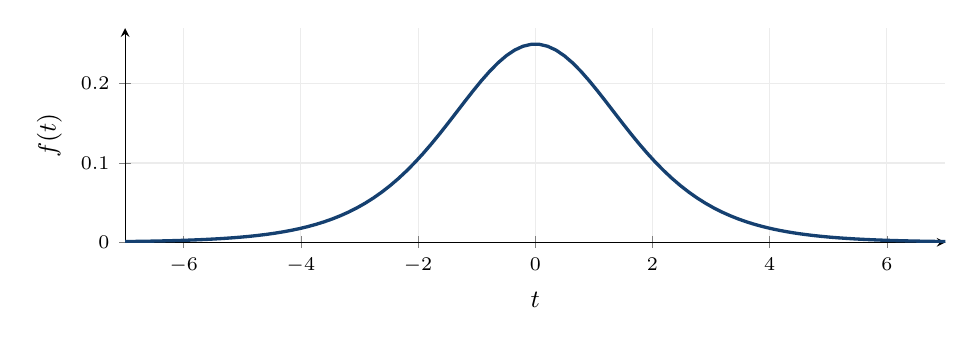
\begin{tikzpicture}
\begin{axis}[base,width=12cm,height=4.3cm,xmin=-7,xmax=7,ymin=0,ymax=.27,xlabel={$t$},ylabel={$f(t)$}]
\addplot[azul,very thick,domain=-7:7]{exp(-abs(x))/(1+exp(-abs(x)))^2};
\end{axis}
\end{tikzpicture}
\caption{Densidad logística del error latente; su simetría explica la igualdad usada en el enlace.}
\end{figure}

\clearpage
\section{Binomial agrupada: cada repetición y cada factor combinatorio}\label{logit71}
Supongamos que para un mismo vector \(x_i\) se observan \(m_i\)
respuestas independientes. El dato \(y_i\) es ahora su suma,
por lo que \(y_i\in\{0,\ldots,m_i\}\).
Cada secuencia con \(y_i\) unos tiene probabilidad
\[
\left[\frac{e^{\sum_jx_{ij}\beta_j}}
{1+e^{\sum_jx_{ij}\beta_j}}\right]^{y_i}
\left[\frac1{1+e^{\sum_jx_{ij}\beta_j}}\right]^{m_i-y_i}.
\]
Hay \(\binom{m_i}{y_i}\) secuencias: se eligen las posiciones de los unos.
Sumar probabilidades iguales produce la distribución binomial.
El factor combinatorio depende de los datos, pero no de los coeficientes.
La log-verosimilitud completa es
\[
\ell(\beta)=\sum_i\left[
\log\binom{m_i}{y_i}
+y_i\sum_jx_{ij}\beta_j
-m_i\log(1+e^{\sum_jx_{ij}\beta_j})\right].
\]
Derivar respecto de \(\beta_l\), dejando \(m_i,y_i,x_{ij}\) fijos, da
\[
\frac{\partial\ell}{\partial\beta_l}
=\sum_i x_{il}\left[
y_i-m_i\frac{e^{\sum_jx_{ij}\beta_j}}
{1+e^{\sum_jx_{ij}\beta_j}}\right].
\]
La segunda derivada conserva el número de repeticiones:
\[
-\frac{\partial^2\ell}{\partial\beta_l\partial\beta_h}
=\sum_i m_i
\frac{e^{\sum_jx_{ij}\beta_j}}
{(1+e^{\sum_jx_{ij}\beta_j})^2}x_{il}x_{ih}.
\]
Esta cuenta coincide con escribir las \(m_i\) filas repetidas
una por una. Agrupar comprime la representación de los datos
sin cambiar su contribución al gradiente o a la curvatura.

La suma de \(m_i\) Bernoulli independientes tiene esperanza igual
a la suma de sus esperanzas y varianza igual a la suma de sus
varianzas. Por tanto,
\[
\E[Y_i\mid x_i]=m_i\frac{e^{\sum_jx_{ij}\beta_j}}{1+e^{\sum_jx_{ij}\beta_j}},
\quad
\Var(Y_i\mid x_i)=m_i\frac{e^{\sum_jx_{ij}\beta_j}}
{(1+e^{\sum_jx_{ij}\beta_j})^2}.
\]
Para la proporción observada \(Y_i/m_i\), la varianza se divide
por \(m_i^2\), de modo que queda la varianza Bernoulli dividida
por \(m_i\). Si dos proporciones iguales provienen de tamaños
de grupo distintos, contienen distinta precisión.

\begin{ejemplo}[Un grupo y solo intercepto]
Con \(m_1=20,y_1=14\), la ecuación del gradiente es
\(14-20e^{\beta_1}/(1+e^{\beta_1})=0\).
Su solución es \(\widehat\beta_1=\log(14/6)\).
La curvatura positiva en ese punto es
\(20(.7)(.3)=4.2\), y la inversa local es \(1/4.2\).
Las constantes \(\log\binom{20}{14}\) no alteran la raíz,
pero sí forman parte de la probabilidad del conteo observado.
\end{ejemplo}
La binomial presupone independencia y una probabilidad común
dentro del grupo. Si hay dependencia, la varianza incluye
covarianzas entre las respuestas; no se obtiene justificadamente
multiplicando una Bernoulli por el tamaño del grupo.

\clearpage
\section{Prueba de score: evaluar el gradiente bajo una restricción}\label{logit72}
La prueba de score pregunta si el gradiente en el modelo
restringido es demasiado grande respecto de su variabilidad.
Considérese primero una hipótesis que fija todos los coeficientes
en \(\beta_0\). Bajo esa hipótesis,
\[
\E[\nabla_\beta\ell(\beta_0)\mid X]=0,\quad
\Cov(\nabla_\beta\ell(\beta_0)\mid X)
=\sum_i\frac{e^{\sum_jx_{ij}\beta_{0j}}}
{(1+e^{\sum_jx_{ij}\beta_{0j}})^2}x_ix_i\T.
\]
Bajo condiciones de límite central y rango completo,
la forma cuadrática
\[
\nabla_\beta\ell(\beta_0)\T
\left[\sum_i\frac{e^{\sum_jx_{ij}\beta_{0j}}}
{(1+e^{\sum_jx_{ij}\beta_{0j}})^2}x_ix_i\T\right]^{-1}
\nabla_\beta\ell(\beta_0)
\]
tiene límite \(\chi^2_k\). La estandarización utiliza la covarianza
del gradiente bajo la hipótesis, y no una covarianza calculada
en un parámetro que todavía no se ha estimado.

Si solo se impone \(\beta_2=0\) en un modelo con intercepto,
primero se estima el intercepto restringido.
Supongamos \(x_{i1}=1\), \(\sum_i y_i\) estrictamente entre cero y \(n\).
La probabilidad restringida es \(\sum_i y_i/n\).
La curvatura relevante para la segunda coordenada,
después de permitir que se ajuste el intercepto, es
\[
\frac{\sum_i y_i}{n}
\left(1-\frac{\sum_i y_i}{n}\right)
\left[\sum_i x_{i2}^2-\frac{(\sum_i x_{i2})^2}{n}\right].
\]
Para derivarla, abrimos el sistema cuadrático de dos parámetros
y completamos el cuadrado en la corrección del intercepto.
La matriz tiene entradas proporcionales a
\(n,\sum_i x_{i2},\sum_i x_{i2}^2\).
Minimizar en la primera corrección resta exactamente
\((\sum_i x_{i2})^2/n\) a la suma de cuadrados de la segunda.
El resultado es también
\(\sum_i(x_{i2}-n^{-1}\sum_r x_{r2})^2\).

El estadístico para una pendiente es entonces
\[
\frac{\left[\sum_i x_{i2}
(y_i-\sum_r y_r/n)\right]^2}
{\frac{\sum_i y_i}{n}(1-\frac{\sum_i y_i}{n})
\left[\sum_i x_{i2}^2-(\sum_i x_{i2})^2/n\right]}.
\]
No hay inversa si todos los \(x_{i2}\) son iguales: esa pendiente
no se distingue del intercepto.

\begin{ejemplo}[Doce datos, modelo con intercepto y \(x_{i2}\)]
El conteo es siete, \(\sum_i x_{i2}=12\),
\(\sum_i x_{i2}^2=50\) y \(\sum_i x_{i2}y_i=11\).
El numerador antes de elevar al cuadrado es \(11-7=4\).
El denominador es \((7/12)(5/12)(50-12)=1330/144\).
El estadístico es \(2304/1330\approx1.73233\).
Este ejemplo restringe el modelo a dos columnas: no trata
\(x_{i3}\) como si nunca hubiera existido en un modelo de tres.
\end{ejemplo}
El resultado \(\chi^2_1\) es asintótico. Una muestra pequeña
no se convierte en normal simplemente por escribir
una forma cuadrática.

\clearpage
\section{Centrar un regresor: equivalencia exacta de las probabilidades}\label{logit73}
Mantengamos \(x_{i1}=1\) y dos pendientes.
Para una constante conocida \(c\), podemos escribir la misma suma como
\[
\beta_1+x_{i2}\beta_2+x_{i3}\beta_3
=(\beta_1+c\beta_2)+(x_{i2}-c)\beta_2+x_{i3}\beta_3.
\]
Los coeficientes en esta representación son
\(\widetilde\beta_1=\beta_1+c\beta_2\),
\(\widetilde\beta_2=\beta_2\), \(\widetilde\beta_3=\beta_3\).
No se cambia el nombre de \(x_{i2}\): se muestra su
valor centrado dentro del producto.
Sustituir la igualdad en cada exponencial prueba
que todas las probabilidades y la verosimilitud coinciden exactamente.

La transformación de coeficientes y su inversa son
\[
\widetilde\beta=
\begin{pmatrix}1&c&0\\0&1&0\\0&0&1\end{pmatrix}\beta,
\qquad
\beta=
\begin{pmatrix}1&-c&0\\0&1&0\\0&0&1\end{pmatrix}\widetilde\beta.
\]
Si los estimadores correspondientes existen y se obtienen
sin penalizar, la igualdad vale para cada muestra:
\(\widehat{\widetilde\beta}_1=\widehat\beta_1+c\widehat\beta_2\).
Para estimadores con momentos finitos, linealidad de esperanza da
\[
\E[\widehat{\widetilde\beta}_1]
=\E[\widehat\beta_1]+c\E[\widehat\beta_2].
\]
Al expandir el cuadrado centrado, la varianza y covarianzas son
\[
\begin{aligned}
\Var(\widehat{\widetilde\beta}_1)
&=\Var(\widehat\beta_1)+2c\Cov(\widehat\beta_1,\widehat\beta_2)
+c^2\Var(\widehat\beta_2),\\
\Cov(\widehat{\widetilde\beta}_1,\widehat{\widetilde\beta}_2)
&=\Cov(\widehat\beta_1,\widehat\beta_2)+c\Var(\widehat\beta_2),\\
\Cov(\widehat{\widetilde\beta}_1,\widehat{\widetilde\beta}_3)
&=\Cov(\widehat\beta_1,\widehat\beta_3)
+c\Cov(\widehat\beta_2,\widehat\beta_3).
\end{aligned}
\]
Las covarianzas de las pendientes no cambian.
La misma transformación se aplica a covarianzas asintóticas,
siempre indicando que son aproximaciones.

En el ejemplo de doce filas, la media de \(x_{i2}\) es uno.
Al usar \(c=1\), el intercepto final pasa de
\(-.02761763\) a \(.45513348\).
Con la matriz local calculada posteriormente,
\[
\widehat{\Var}(\widehat{\widetilde\beta}_1)
=.81823241-2(.10377324)+.14936599=.76005191.
\]
El cambio de intercepto modifica dónde se evalúa la probabilidad
base, pero no modifica ninguna probabilidad individual.

Centrar puede reducir correlación numérica entre columnas.
En logit, la ortogonalidad de curvatura requiere
\(\sum_i e^{\sum_jx_{ij}\beta_j}
(x_{i2}-c)/(1+e^{\sum_jx_{ij}\beta_j})^2=0\),
por lo que el centro adecuado local es una media ponderada.
La media aritmética no asegura esa igualdad salvo que
los factores de curvatura sean iguales o que la suma resulte cero.

\clearpage
\section{Cambiar unidades y transformar toda la covarianza}\label{logit74}
Supongamos que \(x_{i2}\) se mide en una unidad cien veces
más grande. En la nueva representación se utiliza \(x_{i2}/100\).
Para conservar el producto original, se necesita
\(\widetilde\beta_2=100\beta_2\), manteniendo los otros coeficientes.
La igualdad completa es
\[
\beta_1+x_{i2}\beta_2+x_{i3}\beta_3
=\widetilde\beta_1+\frac{x_{i2}}{100}\widetilde\beta_2
+x_{i3}\widetilde\beta_3.
\]
No se puede comparar el tamaño de dos coeficientes
sin considerar las unidades de sus regresores.

Para una transformación lineal explícita,
\[
\widehat{\widetilde\beta}=
\begin{pmatrix}1&0&0\\0&100&0\\0&0&1\end{pmatrix}
\widehat\beta,
\]
la covarianza se transforma multiplicando por esa matriz
a la izquierda y por su transpuesta a la derecha.
Escribiendo todas las entradas,
\[
\Cov(\widehat{\widetilde\beta})=
\begin{pmatrix}
\Var(\widehat\beta_1)&100\Cov(\widehat\beta_1,\widehat\beta_2)&\Cov(\widehat\beta_1,\widehat\beta_3)\\
100\Cov(\widehat\beta_2,\widehat\beta_1)&10000\Var(\widehat\beta_2)&100\Cov(\widehat\beta_2,\widehat\beta_3)\\
\Cov(\widehat\beta_3,\widehat\beta_1)&100\Cov(\widehat\beta_3,\widehat\beta_2)&\Var(\widehat\beta_3)
\end{pmatrix}.
\]
El error estándar de la segunda coordenada se multiplica
por cien, igual que su estimador. El cociente de Wald
para contrastar que esa pendiente es cero permanece igual.

La varianza de una predicción lineal también permanece igual:
\[
(1,x_{i2}/100,x_{i3})
\,\Cov(\widehat{\widetilde\beta})\,
(1,x_{i2}/100,x_{i3})\T
=x_i\T\Cov(\widehat\beta)x_i.
\]
Cada factor cien en la covarianza se cancela con un factor
\(1/100\) en el dato correspondiente.
Este cálculo comprueba invariancia de la incertidumbre
de una misma cantidad observable.

Para un cambio general de unidades y centrado,
se usa una transformación invertible de las columnas.
La verosimilitud sin penalizar depende del mismo producto lineal,
y por tanto sus máximos correspondientes se transforman.
Una penalización \(\sum_j\beta_j^2\) no conserva esa equivalencia:
después de cambiar unidades debería transformarse también
la forma cuadrática de la penalización si se desea el mismo modelo.

La escala influye asimismo en el número de condición del sistema
de Newton. Un coeficiente grande puede ser una consecuencia
de unidades pequeñas del dato. La estabilidad se estudia
con la curvatura y sus direcciones, no únicamente leyendo
los números de los coeficientes.

\clearpage
\section{Mínimos cuadrados locales: QR sin formar productos cruzados}\label{logit75}
En cada paso IRLS, las filas se multiplican por la raíz
de su varianza Bernoulli calculada en los coeficientes actuales.
La matriz que se factoriza tiene fila \(i\)
\[
\frac{e^{\frac12\sum_jx_{ij}\beta_j^{(m)}}}
{1+e^{\sum_jx_{ij}\beta_j^{(m)}}}
(x_{i1},\ldots,x_{ik}).
\]
Su producto transpuesta por sí misma es exactamente
la curvatura positiva de Newton, porque el cuadrado
del factor de fila es \(e^{\sum_jx_{ij}\beta_j^{(m)}}
/(1+e^{\sum_jx_{ij}\beta_j^{(m)}})^2\).

Una factorización QR escribe esa matriz de filas ponderadas
como \(QR\), donde \(Q\T Q=I_k\) y \(R\) es triangular.
Aquí \(Q\) y \(R\) son factores de la descomposición:
no sustituyen el nombre de los datos ni el de una
matriz de productos cruzados.
El vector de la respuesta ponderada tiene entrada
\[
\frac{e^{\frac12\sum_jx_{ij}\beta_j^{(m)}}}
{1+e^{\sum_jx_{ij}\beta_j^{(m)}}}
\left[
\sum_jx_{ij}\beta_j^{(m)}
+\frac{y_i-\frac{e^{\sum_jx_{ij}\beta_j^{(m)}}}
{1+e^{\sum_jx_{ij}\beta_j^{(m)}}}}
{\frac{e^{\sum_jx_{ij}\beta_j^{(m)}}}
{(1+e^{\sum_jx_{ij}\beta_j^{(m)}})^2}}
\right].
\]
Multiplicarlo por \(Q\T\), y resolver con \(R\), obtiene
los nuevos coeficientes sin construir explícitamente
el producto cruzado.

Para probar la equivalencia, descompongamos la respuesta
ponderada en su proyección sobre las columnas de \(Q\)
y su componente ortogonal.
El cuadrado del error es la suma de dos cuadrados:
\[
\|QR\beta-Q Q\T(\text{respuesta ponderada})\|_2^2
+\|(I-QQ\T)(\text{respuesta ponderada})\|_2^2.
\]
El segundo término no depende de \(\beta\).
El primero se minimiza resolviendo
\(R\beta=Q\T(\text{respuesta ponderada})\).
No se ha cambiado la función cuadrática que se minimiza.

Si los valores singulares de las filas ponderadas son
\(s_1\ge\cdots\ge s_k>0\), los autovalores de su
producto cruzado son \(s_1^2,\ldots,s_k^2\).
El número de condición espectral pasa de \(s_1/s_k\)
a \((s_1/s_k)^2\).
Formar productos cruzados puede así agravar la pérdida
de precisión en presencia de columnas casi dependientes.
QR y SVD proporcionan maneras de resolver el mismo
problema local con mejor control de ese efecto.

Una dependencia exacta no se arregla con QR:
produce un factor triangular singular.
Se necesita analizar identificación o introducir una
restricción o penalización explícita.
El algoritmo de álgebra lineal no crea información
que los datos no contienen.

\clearpage
\section{Información, elipses y SVD de las filas ponderadas}\label{logit76}
La aproximación cuadrática de la log-verosimilitud alrededor
del máximo finito es
\[
\ell(\widehat\beta+h)-\ell(\widehat\beta)
\approx-\frac12\sum_i
\frac{e^{\sum_jx_{ij}\widehat\beta_j}}
{(1+e^{\sum_jx_{ij}\widehat\beta_j})^2}
\left(\sum_jx_{ij}h_j\right)^2.
\]
Cada suma interna proyecta el cambio de coeficientes
sobre una fila observada. La caída depende de cómo
esas proyecciones se acumulan, no solo de \(\|h\|_2\).

Si las filas ponderadas se descomponen como \(USV\T\),
las columnas de \(V\) son ortonormales y las entradas
diagonales de \(S\) son los valores singulares.
Para \(h=Vt\),
\[
\sum_i\frac{e^{\sum_jx_{ij}\widehat\beta_j}}
{(1+e^{\sum_jx_{ij}\widehat\beta_j})^2}
\left(\sum_jx_{ij}h_j\right)^2
=\sum_{j=1}^k s_j^2t_j^2.
\]
La superficie de caída constante es una elipse o elipsoide
en coordenadas del parámetro. Sus semiejes son
proporcionales a \(1/s_j\).
Una dirección con pequeño \(s_j\) admite grandes cambios
del coeficiente con poca caída de la log-verosimilitud.

La inversa local de curvatura es
\[
V\diag(s_1^{-2},\ldots,s_k^{-2})V\T.
\]
Su entrada \((l,h)\) es
\(\sum_j V_{lj}V_{hj}/s_j^2\).
Su diagonal mezcla la contribución de todas las direcciones
singulares: no es en general el recíproco de la entrada
diagonal de la curvatura.

En dos coordenadas, considérese la curvatura
\[
\begin{pmatrix}4&2\\2&4\end{pmatrix},
\qquad
\begin{pmatrix}4&2\\2&4\end{pmatrix}^{-1}
=\frac1{12}\begin{pmatrix}4&-2\\-2&4\end{pmatrix}.
\]
Los vectores \((1,1)/\sqrt2\) y \((1,-1)/\sqrt2\)
tienen autovalores seis y dos.
La elipse \(4h_1^2+4h_1h_2+4h_2^2=1\)
tiene semiejes \(1/\sqrt6\) y \(1/\sqrt2\).
La covarianza local cruzada es negativa:
para compensar el aumento de una coordenada,
la otra puede disminuir.

La figura conserva la misma escala en ambos ejes.
Su orientación es consecuencia de los términos cruzados.
Estas elipses son locales: lejos del máximo, la
log-verosimilitud logística no es exactamente cuadrática.

\begin{figure}[H]\centering
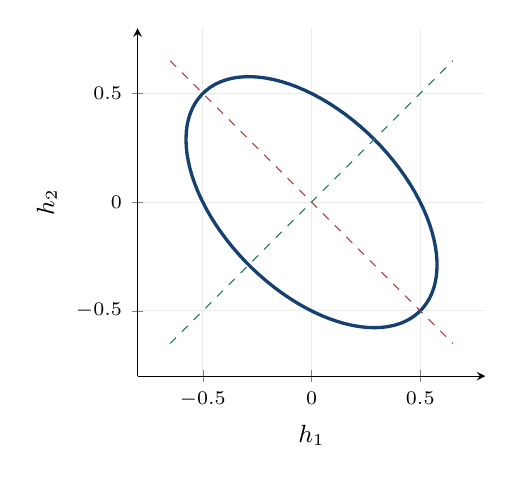
\begin{tikzpicture}
\begin{axis}[base,width=12cm,height=6cm,axis equal image,xmin=-.8,xmax=.8,ymin=-.8,ymax=.8,xlabel={$h_1$},ylabel={$h_2$}]

\addplot[azul,very thick,domain=0:360,variable=\t]
({cos(\t)/sqrt(12)+sin(\t)/2},{cos(\t)/sqrt(12)-sin(\t)/2});
\addplot[verde,dashed] coordinates {(-.65,-.65)(.65,.65)};
\addplot[rojo,dashed] coordinates {(-.65,.65)(.65,-.65)};

\end{axis}
\end{tikzpicture}
\caption{Elipse de caída cuadrática constante y direcciones de curvatura seis y dos.}
\end{figure}

\clearpage
\section{Influencia de una respuesta: derivación implícita del cambio de coeficientes}\label{logit77}
Para estudiar sensibilidad matemática, permitamos temporalmente
que las respuestas varíen como números reales cercanos a los
observados. No se cambia la naturaleza Bernoulli de los datos:
se estudia la función que resuelve las ecuaciones del gradiente.
En una solución finita y de rango completo,
\[
\sum_i x_i\left[
y_i-\frac{e^{\sum_jx_{ij}\widehat\beta_j}}
{1+e^{\sum_jx_{ij}\widehat\beta_j}}\right]=0.
\]
Derivemos esta igualdad respecto de una sola respuesta \(y_r\).
Su derivada directa es \(x_r\).
El cambio indirecto de todas las probabilidades contiene
el Jacobiano respecto de \(\widehat\beta\), por lo que
\[
x_r-\left[
\sum_i\frac{e^{\sum_jx_{ij}\widehat\beta_j}}
{(1+e^{\sum_jx_{ij}\widehat\beta_j})^2}x_ix_i\T
\right]\frac{\partial\widehat\beta}{\partial y_r}=0.
\]
Resolver el sistema produce la derivada exacta local
\[
\frac{\partial\widehat\beta}{\partial y_r}
=\left[
\sum_i\frac{e^{\sum_jx_{ij}\widehat\beta_j}}
{(1+e^{\sum_jx_{ij}\widehat\beta_j})^2}x_ix_i\T
\right]^{-1}x_r.
\]
La condición de inversibilidad es precisamente la que
permite aplicar el teorema de la función implícita.

Si una respuesta cambia una cantidad pequeña \(\delta\),
el cambio de la coordenada \(l\) es aproximadamente
\[
\delta\sum_{h=1}^k
\left(\left[
\sum_i\frac{e^{\sum_jx_{ij}\widehat\beta_j}}
{(1+e^{\sum_jx_{ij}\widehat\beta_j})^2}x_ix_i\T
\right]^{-1}\right)_{lh}x_{rh}.
\]
La aproximación es de primer orden en \(\delta\).
Cambiar un cero por un uno usa \(\delta=1\),
que puede ser demasiado grande para una buena
aproximación y puede incluso inducir separación.
En ese caso hay que volver a estimar y analizar existencia.

Para eliminar una fila, introduzcamos una intensidad
de eliminación \(t\) y restemos \(t\) veces su contribución
a la ecuación del gradiente.
Al derivar en \(t=0\), el cambio inicial es
\[
-\left[
\sum_i\frac{e^{\sum_jx_{ij}\widehat\beta_j}}
{(1+e^{\sum_jx_{ij}\widehat\beta_j})^2}x_ix_i\T
\right]^{-1}x_r
\left[y_r-\frac{e^{\sum_jx_{rj}\widehat\beta_j}}
{1+e^{\sum_jx_{rj}\widehat\beta_j}}\right].
\]
El signo negativo refleja que se retira su fuerza en el gradiente.
Una fila puede tener coordenadas grandes pero discrepancia
pequeña; su influencia inicial sobre la solución puede
entonces ser moderada.
La precisión de esta fórmula depende de que la solución
permanezca en la misma región de curvatura.

\clearpage
\section{Palanca local: diagonal de una proyección y suma igual al rango}\label{logit78}
En las filas ponderadas de IRLS, la proyección ortogonal
sobre el espacio de sus columnas tiene entrada diagonal
\[
\frac{e^{\sum_jx_{ij}\widehat\beta_j}}
{(1+e^{\sum_jx_{ij}\widehat\beta_j})^2}
x_i\T\left[
\sum_r\frac{e^{\sum_jx_{rj}\widehat\beta_j}}
{(1+e^{\sum_jx_{rj}\widehat\beta_j})^2}x_rx_r\T
\right]^{-1}x_i.
\]
Esta cantidad combina el factor Bernoulli de la fila
y su ubicación respecto del diseño completo.
Es la palanca del problema cuadrático local,
no una probabilidad de que la fila sea correcta.

Para demostrar sus propiedades, escribamos la proyección
como \(QQ\T\), usando el factor ortonormal del QR.
Su entrada diagonal es
\(\sum_{j=1}^k Q_{ij}^2\), que es no negativa.
La proyección no aumenta normas, por lo que
\(\|QQ\T e_i\|_2^2\le\|e_i\|_2^2=1\).
Como la proyección es simétrica e idempotente,
esa norma al cuadrado coincide con la entrada diagonal.
Así cada palanca está entre cero y uno.

La suma de todas las entradas diagonales es
\[
\sum_{i=1}^n\sum_{j=1}^k Q_{ij}^2
=\sum_{j=1}^k\sum_{i=1}^n Q_{ij}^2=k,
\]
porque cada columna de \(Q\) tiene norma uno.
La palanca promedio es \(k/n\), aunque algunas filas
puedan concentrar mucha más que otras.
Si hay rango menor, la suma es el rango real.

Para dos filas distintas, la entrada cruzada de la proyección es
\[
\frac{e^{\frac12\sum_jx_{ij}\widehat\beta_j}}
{1+e^{\sum_jx_{ij}\widehat\beta_j}}
\frac{e^{\frac12\sum_jx_{rj}\widehat\beta_j}}
{1+e^{\sum_jx_{rj}\widehat\beta_j}}
x_i\T\left[
\sum_s\frac{e^{\sum_jx_{sj}\widehat\beta_j}}
{(1+e^{\sum_jx_{sj}\widehat\beta_j})^2}x_sx_s\T
\right]^{-1}x_r.
\]
La desigualdad de Cauchy--Schwarz sobre las filas de \(Q\)
acota su valor absoluto por la raíz del producto
de las dos palancas diagonales.
Las respuestas independientes pueden así compartir
incertidumbre en sus predicciones estimadas.

Con ridge, la matriz correspondiente incorpora
\(\lambda I_k\) antes de invertir.
Ya no es una proyección idempotente:
sus autovalores son \(s_j^2/(s_j^2+\lambda)\).
Su traza es una suma de números entre cero y uno,
que mide grados de libertad locales reducidos.
No se debe conservar la identidad de traza igual a \(k\)
después de introducir esa penalización.

\clearpage
\section{No colapsabilidad: por qué una pendiente marginal puede cambiar}\label{logit79}
Consideremos \(x_{i1}=1\) y dos regresores binarios,
con coeficientes \(\beta_1=0\), \(\beta_2=\log2\),
\(\beta_3=\log3\). La probabilidad condicional es
\[
\frac{\exp(x_{i2}\log2+x_{i3}\log3)}
{1+\exp(x_{i2}\log2+x_{i3}\log3)}.
\]
Para \(x_{i2}=0\), las probabilidades al variar \(x_{i3}\)
entre cero y uno son \(1/2\) y \(3/4\).
Para \(x_{i2}=1\), son \(2/3\) y \(6/7\).
En cada valor de \(x_{i3}\), el odds ratio asociado a
cambiar \(x_{i2}\) de cero a uno es exactamente dos.

Supongamos que \(x_{i3}\) es independiente de \(x_{i2}\)
y vale cero o uno con probabilidad \(1/2\).
La ley de probabilidad total da
\[
\begin{aligned}
\Prob(Y_i=1\mid x_{i2}=0)&=\tfrac12(\tfrac12+\tfrac34)=\tfrac58,\\
\Prob(Y_i=1\mid x_{i2}=1)&=\tfrac12(\tfrac23+\tfrac67)=\tfrac{16}{21}.
\end{aligned}
\]
Los odds marginales son \(5/3\) y \(16/5\).
Su cociente es
\[
\frac{16/5}{5/3}=\frac{48}{25}=1.92,
\]
distinto de dos, a pesar de la independencia de los regresores.
En un modelo marginal con un único regresor binario,
el intercepto sería \(\log(5/3)\) y la pendiente
sería \(\log(48/25)\), aproximadamente \(.65232519\).

La razón no es un fallo de álgebra:
promediar probabilidades y transformar a odds
no son operaciones que puedan intercambiarse.
En general,
\[
\frac{\E\left[e^{\beta_1+x_{i2}\beta_2+x_{i3}\beta_3}/
(1+e^{\beta_1+x_{i2}\beta_2+x_{i3}\beta_3})\mid x_{i2}\right]}
{1-\E\left[e^{\beta_1+x_{i2}\beta_2+x_{i3}\beta_3}/
(1+e^{\beta_1+x_{i2}\beta_2+x_{i3}\beta_3})\mid x_{i2}\right]}
\]
no coincide con el exponencial de la media del producto lineal.
No puede deducirse una pendiente marginal simplemente
eliminando \(\beta_3x_{i3}\) de la fórmula condicional.

El coeficiente logit describe odds condicionales
dados todos los regresores incluidos.
Un cambio al agregar o retirar una variable puede reflejar
un cambio de la cantidad condicionada, además de otros
problemas de especificación.
La comparación matemática exige precisar cuál
distribución de \(x_{i3}\) se está promediando.

\begin{figure}[H]\centering
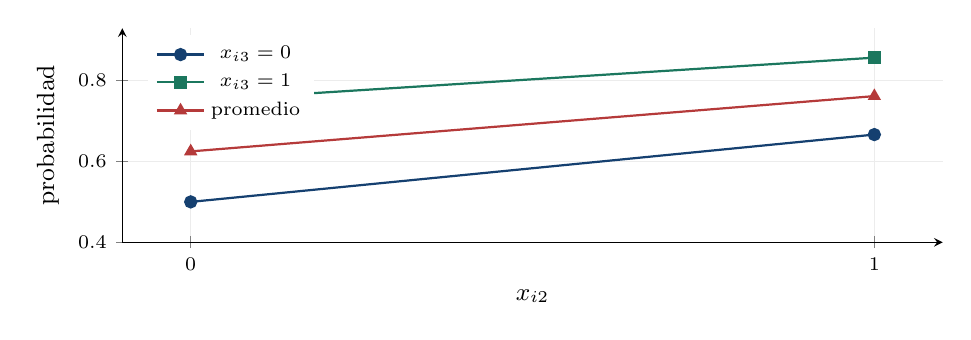
\begin{tikzpicture}
\begin{axis}[base,width=12cm,height=4.3cm,xmin=-.1,xmax=1.1,ymin=.4,ymax=.93,xtick={0,1},xlabel={$x_{i2}$},ylabel={probabilidad},legend pos=north west]

\addplot[azul,thick,mark=*] coordinates {(0,.5)(1,.666666667)};
\addplot[verde,thick,mark=square*] coordinates {(0,.75)(1,.857142857)};
\addplot[rojo,thick,mark=triangle*] coordinates {(0,.625)(1,.761904762)};
\legend{$x_{i3}=0$,$x_{i3}=1$,promedio}

\end{axis}
\end{tikzpicture}
\caption{Probabilidades condicionales y su promedio; los odds se transforman después de promediar.}
\end{figure}

\clearpage
\section{Selección por respuesta: derivar el cambio de intercepto}\label{logit80}
Supongamos que una observación entra en la muestra con
probabilidad \(s_1>0\) si \(Y_i=1\), y con probabilidad
\(s_0>0\) si \(Y_i=0\). Condicionalmente en la respuesta,
la selección no depende de \(x_i\).
Denotemos por \(S_i=1\) el evento de inclusión.
Bayes da
\[
\Prob(Y_i=1\mid x_i,S_i=1)
=\frac{s_1\Prob(Y_i=1\mid x_i)}
{s_1\Prob(Y_i=1\mid x_i)+s_0\Prob(Y_i=0\mid x_i)}.
\]
La probabilidad del cero tiene el mismo denominador,
y numerador \(s_0\Prob(Y_i=0\mid x_i)\).
Dividir ambas probabilidades cancela ese denominador:
\[
\frac{\Prob(Y_i=1\mid x_i,S_i=1)}
{\Prob(Y_i=0\mid x_i,S_i=1)}
=\frac{s_1}{s_0}
\frac{\Prob(Y_i=1\mid x_i)}{\Prob(Y_i=0\mid x_i)}.
\]
Si el modelo poblacional es logit, tomar logaritmos produce
\[
\log\frac{\Prob(Y_i=1\mid x_i,S_i=1)}
{1-\Prob(Y_i=1\mid x_i,S_i=1)}
=\log(s_1/s_0)+\beta_1+\sum_{j=2}^k x_{ij}\beta_j.
\]
El intercepto cambia en \(\log(s_1/s_0)\);
las pendientes de la probabilidad condicional seleccionada
son las mismas bajo estas condiciones concretas.

La probabilidad muestral también puede comprobarse
sustituyendo la fracción logística:
\[
\Prob(Y_i=1\mid x_i,S_i=1)
=\frac{\exp[\log(s_1/s_0)+\sum_jx_{ij}\beta_j]}
{1+\exp[\log(s_1/s_0)+\sum_jx_{ij}\beta_j]}.
\]
Por ejemplo, si \(s_1=1,s_0=1/4\), el intercepto
aumenta en \(\log4\).
Una probabilidad poblacional \(1/2\) se convierte
en probabilidad muestral \(4/5\).

Si se conocen las probabilidades de selección,
restar el desplazamiento corrige el intercepto del modelo
condicional estimado en esa muestra.
Para calcular incertidumbre hay que considerar también
si \(s_1,s_0\) son conocidos o estimados:
en el segundo caso, su variabilidad y covarianza con
el estimador deben incluirse mediante una expansión conjunta.

Esta identidad describe la distribución de una observación
seleccionada por el mecanismo indicado.
Un diseño que fija exactamente números de casos y controles
requiere tratar su esquema de muestreo para formular
una verosimilitud y errores estándar apropiados.
Tampoco se conserva la conclusión si la razón de selección
depende de \(x_i\) de una manera omitida del modelo.

\clearpage
\section{Pérdida logarítmica y Brier: demostrar qué probabilidad minimizan}\label{logit81}
Sea \(q=\Prob(Y_i=1\mid x_i)\) la probabilidad verdadera
y sea \(r\in(0,1)\) una probabilidad anunciada.
Estas letras designan probabilidades escalares de esta
demostración; no reemplazan los \(x_{ij}\) de ningún cálculo.
La pérdida logarítmica esperada es
\[
-q\log r-(1-q)\log(1-r).
\]
Su derivada es
\[
-\frac qr+\frac{1-q}{1-r}
=\frac{r-q}{r(1-r)}.
\]
Es negativa para \(r<q\) y positiva para \(r>q\).
Por tanto su mínimo es la probabilidad verdadera.
Esta propiedad explica por qué maximizar la verosimilitud
equivale a ajustar probabilidades usando una pérdida
que tiene el objetivo correcto en población.

La pérdida cuadrática de Brier es \((Y_i-r)^2\).
Su esperanza, abriendo los dos eventos, es
\[
q(1-r)^2+(1-q)r^2
=q-2qr+r^2
=q(1-q)+(r-q)^2.
\]
La parte \(q(1-q)\) no depende de la probabilidad anunciada.
La otra parte es no negativa y se anula solamente en \(r=q\).
Ambas pérdidas identifican la probabilidad correcta,
pero penalizan errores de maneras diferentes.

La pérdida logarítmica al observar un uno es \(-\log r\),
que diverge cuando \(r\downarrow0\).
La pérdida Brier en ese evento es \((1-r)^2\), acotada por uno.
Por ello probabilidades extremadamente equivocadas pueden
dominar la pérdida logarítmica de una muestra.

Un clasificador que anuncia uno si \(r>1/2\) reduce
toda esa información a una decisión.
Para \(q=.51\) y \(q=.99\), la decisión es la misma,
pero la incertidumbre de la respuesta es muy distinta.
Evaluar una decisión y evaluar una probabilidad son
problemas matemáticos distintos.

Si el costo de predecir uno cuando el dato es cero
es \(c_{01}>0\), y el de predecir cero cuando el dato
es uno es \(c_{10}>0\), los costos esperados son
\(c_{01}(1-q)\) y \(c_{10}q\).
Se predice uno cuando
\[
c_{01}(1-q)<c_{10}q
\quad\Longleftrightarrow\quad
q>\frac{c_{01}}{c_{01}+c_{10}}.
\]
El umbral depende de los costos.
No se deduce que siempre deba ser \(1/2\) a partir
de la forma de la función logística.

\begin{figure}[H]\centering
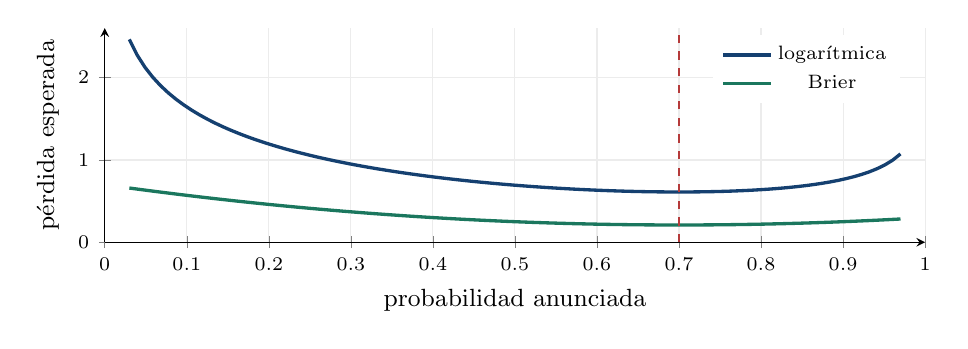
\begin{tikzpicture}
\begin{axis}[base,width=12cm,height=4.3cm,xmin=0,xmax=1,ymin=0,ymax=2.6,xlabel={probabilidad anunciada},ylabel={pérdida esperada},legend pos=north east]

\addplot[azul,very thick,domain=.03:.97]{-.7*ln(x)-.3*ln(1-x)};
\addplot[verde,very thick,domain=.03:.97]{.7*(1-x)^2+.3*x^2};
\addplot[rojo,dashed] coordinates {(.7,0)(.7,2.6)};
\legend{logarítmica,Brier}

\end{axis}
\end{tikzpicture}
\caption{Pérdidas esperadas para probabilidad verdadera \(q=.7\); ambas tienen mínimo en .7.}
\end{figure}

\clearpage
\section{Laboratorio original: doce filas y una solución finita comprobable}\label{logit82}
Este laboratorio conserva exactamente los doce pares del archivo
proporcionado. Se muestran todas las filas antes de agregarlas.
La primera columna vale uno y genera el intercepto.
Las otras dos columnas son datos numéricos de cada observación,
no símbolos para ocultar productos.
\[
X=\begin{pmatrix}1&-2&0\\1&-1&1\\1&0&0\\1&1&1\\1&2&0\\1&3&1\\1&-1&1\\1&0&0\\1&1&2\\1&2&0\\1&3&1\\1&4&0\end{pmatrix},\qquad y=\begin{pmatrix}0\\0\\1\\0\\1\\1\\1\\0\\1\\1\\0\\1\end{pmatrix}.
\]

Cada fila de \(X\) es \(x_i\T\), mientras que \(x_i\) es una columna.
Por eso el producto \(x_ix_i\T\) tiene dimensión \(3\times3\)
y el producto \(x_i\T\beta\) tiene dimensión uno.
La orientación determina qué operación es una matriz y cuál
es un producto escalar.

Las filas 2 y 7 tienen el mismo vector \((1,-1,1)\),
pero respuestas distintas. Las filas 3 y 8 comparten
\((1,0,0)\), también con respuestas opuestas.
Las filas 6 y 11 comparten \((1,3,1)\) con respuestas opuestas.
Una dirección de separación débil tendría que cumplir
a la vez ambas desigualdades en cada par. Por ello
debería ser ortogonal a los tres vectores:
\[
\begin{pmatrix}1&-1&1\\1&0&0\\1&3&1\end{pmatrix}v=0.
\]
El determinante es \(4\), no cero.
La única dirección es \(v=0\).
No existe dirección de separación completa o cuasiseparación.
Además, esos tres vectores prueban rango tres.
Con las demostraciones previas, el máximo ordinario
existe, es finito y es único para estos datos concretos.

Las sumas que se necesitan para la curvatura inicial son
\[
\sum_i x_{i1}^2=12,\quad
\sum_i x_{i2}=12,\quad
\sum_i x_{i3}=7,\quad
\sum_i x_{i2}^2=50,\quad
\sum_i x_{i2}x_{i3}=7,\quad
\sum_i x_{i3}^2=9.
\]
En el vector de productos con respuestas,
\(\sum_i y_i=7\), \(\sum_i x_{i2}y_i=11\),
\(\sum_i x_{i3}y_i=4\).
Estos números se reconstruyen fila por fila en las unidades siguientes.

Que el máximo exista en esta realización no garantiza
que exista en toda muestra posible con el mismo diseño.
Las configuraciones con todas las respuestas cero o todas uno
siguen siendo eventos con probabilidad positiva bajo
parámetros finitos.

\clearpage
\section{Fila 1: probabilidad, tres derivadas y nueve productos}\label{logit83}
La fila que se desarrolla aquí es
\[
x_{1}=\begin{pmatrix}1\\-2\\0\end{pmatrix},\qquad y_{1}=0.
\]

El producto que entra en su probabilidad, sin abreviarlo, es
\[
x_{1}\T\beta=\beta_1+(-2)\beta_2+(0)\beta_3.
\]

La contribución de esta observación a la log-verosimilitud
y su vector de derivadas son, respectivamente,
\[
\begin{aligned}
&(0)\bigl[\beta_1+(-2)\beta_2+(0)\beta_3\bigr]-\log\bigl(1+e^{\beta_1+(-2)\beta_2+(0)\beta_3}\bigr),\\&\left[0-\frac{e^{\beta_1+(-2)\beta_2+(0)\beta_3}}{1+e^{\beta_1+(-2)\beta_2+(0)\beta_3}}\right]\begin{pmatrix}1\\-2\\0\end{pmatrix}.\end{aligned}
\]

En \(\beta^{(0)}=(0,0,0)\T\), la probabilidad es \(1/2\);
la contribución al logaritmo es \(-\log2\), independientemente
del cero o uno observado. El gradiente de esta fila es
\[
\left(0-\frac12\right)\begin{pmatrix}1\\-2\\0\end{pmatrix}=\begin{pmatrix}\frac{-1}{2}\\1\\0\end{pmatrix}.
\]
Al observar un cero, la discrepancia inicial es negativa: el dato empuja el producto lineal hacia abajo. Una coordenada negativa del regresor invierte el signo de esa coordenada del gradiente.

El producto exterior se obtiene multiplicando cada coordenada
de la columna por cada coordenada de la fila transpuesta:
\[
x_{1}x_{1}\T=\begin{pmatrix}1&-2&0\\-2&4&0\\0&0&0\end{pmatrix}.
\]

El negativo de la Hessiana de esta fila es \(1/4\)
veces esta matriz en el inicio. Tiene rango uno:
todas sus columnas son múltiplos de \(x_i\).
Una fila contribuye a nueve entradas, pero aporta
solo una dirección independiente de curvatura.

Para \(\beta=(.2,.3,-.1)\T\), el producto vale
\[
(1)(0.20000000)+(-2)(0.30000000)+(0)(-0.10000000)=-0.40000000.
\]
\[
\Prob_\beta(Y_{1}=1\mid x_{1})=\frac{e^{-0.40000000}}{1+e^{-0.40000000}}=0.40131234.
\]

El vector de derivadas y la curvatura positiva aportada
en ese punto son
\[
\begin{pmatrix}-0.40131234\\0.80262468\\0\end{pmatrix},\qquad 0.24026075\,\begin{pmatrix}1&-2&0\\-2&4&0\\0&0&0\end{pmatrix}.
\]

Aquí se ha cambiado el parámetro y por ello el peso de
curvatura cambia, aunque los nueve productos de datos
permanecen iguales.
Al aplicar la primera corrección común calculada con las doce filas,
la probabilidad de esta observación pasa a
\[
(1)(-0.048171)+(-2)(0.421053)+(0)(-0.067797)=-0.89027654.
\]
\[
\frac{e^{-0.89027654}}{1+e^{-0.89027654}}\approx0.29105276.
\]

No se estima un coeficiente diferente para cada fila.
La corrección se obtiene sumando todos los gradientes y todas
las curvaturas antes de resolver un único sistema de tres coordenadas.
Esta distinción conserva los términos cruzados que se perderían
si cada fila se ajustara separadamente.

\clearpage
\section{Fila 2: probabilidad, tres derivadas y nueve productos}\label{logit84}
La fila que se desarrolla aquí es
\[
x_{2}=\begin{pmatrix}1\\-1\\1\end{pmatrix},\qquad y_{2}=0.
\]

El producto que entra en su probabilidad, sin abreviarlo, es
\[
x_{2}\T\beta=\beta_1+(-1)\beta_2+(1)\beta_3.
\]

La contribución de esta observación a la log-verosimilitud
y su vector de derivadas son, respectivamente,
\[
\begin{aligned}
&(0)\bigl[\beta_1+(-1)\beta_2+(1)\beta_3\bigr]-\log\bigl(1+e^{\beta_1+(-1)\beta_2+(1)\beta_3}\bigr),\\&\left[0-\frac{e^{\beta_1+(-1)\beta_2+(1)\beta_3}}{1+e^{\beta_1+(-1)\beta_2+(1)\beta_3}}\right]\begin{pmatrix}1\\-1\\1\end{pmatrix}.\end{aligned}
\]

En \(\beta^{(0)}=(0,0,0)\T\), la probabilidad es \(1/2\);
la contribución al logaritmo es \(-\log2\), independientemente
del cero o uno observado. El gradiente de esta fila es
\[
\left(0-\frac12\right)\begin{pmatrix}1\\-1\\1\end{pmatrix}=\begin{pmatrix}\frac{-1}{2}\\\frac{1}{2}\\\frac{-1}{2}\end{pmatrix}.
\]
Al observar un cero, la discrepancia inicial es negativa: el dato empuja el producto lineal hacia abajo. Una coordenada negativa del regresor invierte el signo de esa coordenada del gradiente.

El producto exterior se obtiene multiplicando cada coordenada
de la columna por cada coordenada de la fila transpuesta:
\[
x_{2}x_{2}\T=\begin{pmatrix}1&-1&1\\-1&1&-1\\1&-1&1\end{pmatrix}.
\]

El negativo de la Hessiana de esta fila es \(1/4\)
veces esta matriz en el inicio. Tiene rango uno:
todas sus columnas son múltiplos de \(x_i\).
Una fila contribuye a nueve entradas, pero aporta
solo una dirección independiente de curvatura.

Para \(\beta=(.2,.3,-.1)\T\), el producto vale
\[
(1)(0.20000000)+(-1)(0.30000000)+(1)(-0.10000000)=-0.20000000.
\]
\[
\Prob_\beta(Y_{2}=1\mid x_{2})=\frac{e^{-0.20000000}}{1+e^{-0.20000000}}=0.45016600.
\]

El vector de derivadas y la curvatura positiva aportada
en ese punto son
\[
\begin{pmatrix}-0.45016600\\0.45016600\\-0.45016600\end{pmatrix},\qquad 0.24751657\,\begin{pmatrix}1&-1&1\\-1&1&-1\\1&-1&1\end{pmatrix}.
\]

Aquí se ha cambiado el parámetro y por ello el peso de
curvatura cambia, aunque los nueve productos de datos
permanecen iguales.
Al aplicar la primera corrección común calculada con las doce filas,
la probabilidad de esta observación pasa a
\[
(1)(-0.048171)+(-1)(0.421053)+(1)(-0.067797)=-0.53702052.
\]
\[
\frac{e^{-0.53702052}}{1+e^{-0.53702052}}\approx0.36888096.
\]

No se estima un coeficiente diferente para cada fila.
La corrección se obtiene sumando todos los gradientes y todas
las curvaturas antes de resolver un único sistema de tres coordenadas.
Esta distinción conserva los términos cruzados que se perderían
si cada fila se ajustara separadamente.

\clearpage
\section{Fila 3: probabilidad, tres derivadas y nueve productos}\label{logit85}
La fila que se desarrolla aquí es
\[
x_{3}=\begin{pmatrix}1\\0\\0\end{pmatrix},\qquad y_{3}=1.
\]

El producto que entra en su probabilidad, sin abreviarlo, es
\[
x_{3}\T\beta=\beta_1+(0)\beta_2+(0)\beta_3.
\]

La contribución de esta observación a la log-verosimilitud
y su vector de derivadas son, respectivamente,
\[
\begin{aligned}
&(1)\bigl[\beta_1+(0)\beta_2+(0)\beta_3\bigr]-\log\bigl(1+e^{\beta_1+(0)\beta_2+(0)\beta_3}\bigr),\\&\left[1-\frac{e^{\beta_1+(0)\beta_2+(0)\beta_3}}{1+e^{\beta_1+(0)\beta_2+(0)\beta_3}}\right]\begin{pmatrix}1\\0\\0\end{pmatrix}.\end{aligned}
\]

En \(\beta^{(0)}=(0,0,0)\T\), la probabilidad es \(1/2\);
la contribución al logaritmo es \(-\log2\), independientemente
del cero o uno observado. El gradiente de esta fila es
\[
\left(1-\frac12\right)\begin{pmatrix}1\\0\\0\end{pmatrix}=\begin{pmatrix}\frac{1}{2}\\0\\0\end{pmatrix}.
\]
Al observar un uno, la discrepancia inicial es positiva: el dato empuja el producto lineal hacia arriba. Una coordenada negativa del regresor invierte el signo de esa coordenada del gradiente.

El producto exterior se obtiene multiplicando cada coordenada
de la columna por cada coordenada de la fila transpuesta:
\[
x_{3}x_{3}\T=\begin{pmatrix}1&0&0\\0&0&0\\0&0&0\end{pmatrix}.
\]

El negativo de la Hessiana de esta fila es \(1/4\)
veces esta matriz en el inicio. Tiene rango uno:
todas sus columnas son múltiplos de \(x_i\).
Una fila contribuye a nueve entradas, pero aporta
solo una dirección independiente de curvatura.

Para \(\beta=(.2,.3,-.1)\T\), el producto vale
\[
(1)(0.20000000)+(0)(0.30000000)+(0)(-0.10000000)=0.20000000.
\]
\[
\Prob_\beta(Y_{3}=1\mid x_{3})=\frac{e^{0.20000000}}{1+e^{0.20000000}}=0.54983400.
\]

El vector de derivadas y la curvatura positiva aportada
en ese punto son
\[
\begin{pmatrix}0.45016600\\0\\0\end{pmatrix},\qquad 0.24751657\,\begin{pmatrix}1&0&0\\0&0&0\\0&0&0\end{pmatrix}.
\]

Aquí se ha cambiado el parámetro y por ello el peso de
curvatura cambia, aunque los nueve productos de datos
permanecen iguales.
Al aplicar la primera corrección común calculada con las doce filas,
la probabilidad de esta observación pasa a
\[
(1)(-0.048171)+(0)(0.421053)+(0)(-0.067797)=-0.04817128.
\]
\[
\frac{e^{-0.04817128}}{1+e^{-0.04817128}}\approx0.48795951.
\]

No se estima un coeficiente diferente para cada fila.
La corrección se obtiene sumando todos los gradientes y todas
las curvaturas antes de resolver un único sistema de tres coordenadas.
Esta distinción conserva los términos cruzados que se perderían
si cada fila se ajustara separadamente.

\clearpage
\section{Fila 4: probabilidad, tres derivadas y nueve productos}\label{logit86}
La fila que se desarrolla aquí es
\[
x_{4}=\begin{pmatrix}1\\1\\1\end{pmatrix},\qquad y_{4}=0.
\]

El producto que entra en su probabilidad, sin abreviarlo, es
\[
x_{4}\T\beta=\beta_1+(1)\beta_2+(1)\beta_3.
\]

La contribución de esta observación a la log-verosimilitud
y su vector de derivadas son, respectivamente,
\[
\begin{aligned}
&(0)\bigl[\beta_1+(1)\beta_2+(1)\beta_3\bigr]-\log\bigl(1+e^{\beta_1+(1)\beta_2+(1)\beta_3}\bigr),\\&\left[0-\frac{e^{\beta_1+(1)\beta_2+(1)\beta_3}}{1+e^{\beta_1+(1)\beta_2+(1)\beta_3}}\right]\begin{pmatrix}1\\1\\1\end{pmatrix}.\end{aligned}
\]

En \(\beta^{(0)}=(0,0,0)\T\), la probabilidad es \(1/2\);
la contribución al logaritmo es \(-\log2\), independientemente
del cero o uno observado. El gradiente de esta fila es
\[
\left(0-\frac12\right)\begin{pmatrix}1\\1\\1\end{pmatrix}=\begin{pmatrix}\frac{-1}{2}\\\frac{-1}{2}\\\frac{-1}{2}\end{pmatrix}.
\]
Al observar un cero, la discrepancia inicial es negativa: el dato empuja el producto lineal hacia abajo. Una coordenada negativa del regresor invierte el signo de esa coordenada del gradiente.

El producto exterior se obtiene multiplicando cada coordenada
de la columna por cada coordenada de la fila transpuesta:
\[
x_{4}x_{4}\T=\begin{pmatrix}1&1&1\\1&1&1\\1&1&1\end{pmatrix}.
\]

El negativo de la Hessiana de esta fila es \(1/4\)
veces esta matriz en el inicio. Tiene rango uno:
todas sus columnas son múltiplos de \(x_i\).
Una fila contribuye a nueve entradas, pero aporta
solo una dirección independiente de curvatura.

Para \(\beta=(.2,.3,-.1)\T\), el producto vale
\[
(1)(0.20000000)+(1)(0.30000000)+(1)(-0.10000000)=0.40000000.
\]
\[
\Prob_\beta(Y_{4}=1\mid x_{4})=\frac{e^{0.40000000}}{1+e^{0.40000000}}=0.59868766.
\]

El vector de derivadas y la curvatura positiva aportada
en ese punto son
\[
\begin{pmatrix}-0.59868766\\-0.59868766\\-0.59868766\end{pmatrix},\qquad 0.24026075\,\begin{pmatrix}1&1&1\\1&1&1\\1&1&1\end{pmatrix}.
\]

Aquí se ha cambiado el parámetro y por ello el peso de
curvatura cambia, aunque los nueve productos de datos
permanecen iguales.
Al aplicar la primera corrección común calculada con las doce filas,
la probabilidad de esta observación pasa a
\[
(1)(-0.048171)+(1)(0.421053)+(1)(-0.067797)=0.30508475.
\]
\[
\frac{e^{0.30508475}}{1+e^{0.30508475}}\approx0.57568505.
\]

No se estima un coeficiente diferente para cada fila.
La corrección se obtiene sumando todos los gradientes y todas
las curvaturas antes de resolver un único sistema de tres coordenadas.
Esta distinción conserva los términos cruzados que se perderían
si cada fila se ajustara separadamente.

\clearpage
\section{Fila 5: probabilidad, tres derivadas y nueve productos}\label{logit87}
La fila que se desarrolla aquí es
\[
x_{5}=\begin{pmatrix}1\\2\\0\end{pmatrix},\qquad y_{5}=1.
\]

El producto que entra en su probabilidad, sin abreviarlo, es
\[
x_{5}\T\beta=\beta_1+(2)\beta_2+(0)\beta_3.
\]

La contribución de esta observación a la log-verosimilitud
y su vector de derivadas son, respectivamente,
\[
\begin{aligned}
&(1)\bigl[\beta_1+(2)\beta_2+(0)\beta_3\bigr]-\log\bigl(1+e^{\beta_1+(2)\beta_2+(0)\beta_3}\bigr),\\&\left[1-\frac{e^{\beta_1+(2)\beta_2+(0)\beta_3}}{1+e^{\beta_1+(2)\beta_2+(0)\beta_3}}\right]\begin{pmatrix}1\\2\\0\end{pmatrix}.\end{aligned}
\]

En \(\beta^{(0)}=(0,0,0)\T\), la probabilidad es \(1/2\);
la contribución al logaritmo es \(-\log2\), independientemente
del cero o uno observado. El gradiente de esta fila es
\[
\left(1-\frac12\right)\begin{pmatrix}1\\2\\0\end{pmatrix}=\begin{pmatrix}\frac{1}{2}\\1\\0\end{pmatrix}.
\]
Al observar un uno, la discrepancia inicial es positiva: el dato empuja el producto lineal hacia arriba. Una coordenada negativa del regresor invierte el signo de esa coordenada del gradiente.

El producto exterior se obtiene multiplicando cada coordenada
de la columna por cada coordenada de la fila transpuesta:
\[
x_{5}x_{5}\T=\begin{pmatrix}1&2&0\\2&4&0\\0&0&0\end{pmatrix}.
\]

El negativo de la Hessiana de esta fila es \(1/4\)
veces esta matriz en el inicio. Tiene rango uno:
todas sus columnas son múltiplos de \(x_i\).
Una fila contribuye a nueve entradas, pero aporta
solo una dirección independiente de curvatura.

Para \(\beta=(.2,.3,-.1)\T\), el producto vale
\[
(1)(0.20000000)+(2)(0.30000000)+(0)(-0.10000000)=0.80000000.
\]
\[
\Prob_\beta(Y_{5}=1\mid x_{5})=\frac{e^{0.80000000}}{1+e^{0.80000000}}=0.68997448.
\]

El vector de derivadas y la curvatura positiva aportada
en ese punto son
\[
\begin{pmatrix}0.31002552\\0.62005104\\0\end{pmatrix},\qquad 0.21390970\,\begin{pmatrix}1&2&0\\2&4&0\\0&0&0\end{pmatrix}.
\]

Aquí se ha cambiado el parámetro y por ello el peso de
curvatura cambia, aunque los nueve productos de datos
permanecen iguales.
Al aplicar la primera corrección común calculada con las doce filas,
la probabilidad de esta observación pasa a
\[
(1)(-0.048171)+(2)(0.421053)+(0)(-0.067797)=0.79393399.
\]
\[
\frac{e^{0.79393399}}{1+e^{0.79393399}}\approx0.68867541.
\]

No se estima un coeficiente diferente para cada fila.
La corrección se obtiene sumando todos los gradientes y todas
las curvaturas antes de resolver un único sistema de tres coordenadas.
Esta distinción conserva los términos cruzados que se perderían
si cada fila se ajustara separadamente.

\clearpage
\section{Fila 6: probabilidad, tres derivadas y nueve productos}\label{logit88}
La fila que se desarrolla aquí es
\[
x_{6}=\begin{pmatrix}1\\3\\1\end{pmatrix},\qquad y_{6}=1.
\]

El producto que entra en su probabilidad, sin abreviarlo, es
\[
x_{6}\T\beta=\beta_1+(3)\beta_2+(1)\beta_3.
\]

La contribución de esta observación a la log-verosimilitud
y su vector de derivadas son, respectivamente,
\[
\begin{aligned}
&(1)\bigl[\beta_1+(3)\beta_2+(1)\beta_3\bigr]-\log\bigl(1+e^{\beta_1+(3)\beta_2+(1)\beta_3}\bigr),\\&\left[1-\frac{e^{\beta_1+(3)\beta_2+(1)\beta_3}}{1+e^{\beta_1+(3)\beta_2+(1)\beta_3}}\right]\begin{pmatrix}1\\3\\1\end{pmatrix}.\end{aligned}
\]

En \(\beta^{(0)}=(0,0,0)\T\), la probabilidad es \(1/2\);
la contribución al logaritmo es \(-\log2\), independientemente
del cero o uno observado. El gradiente de esta fila es
\[
\left(1-\frac12\right)\begin{pmatrix}1\\3\\1\end{pmatrix}=\begin{pmatrix}\frac{1}{2}\\\frac{3}{2}\\\frac{1}{2}\end{pmatrix}.
\]
Al observar un uno, la discrepancia inicial es positiva: el dato empuja el producto lineal hacia arriba. Una coordenada negativa del regresor invierte el signo de esa coordenada del gradiente.

El producto exterior se obtiene multiplicando cada coordenada
de la columna por cada coordenada de la fila transpuesta:
\[
x_{6}x_{6}\T=\begin{pmatrix}1&3&1\\3&9&3\\1&3&1\end{pmatrix}.
\]

El negativo de la Hessiana de esta fila es \(1/4\)
veces esta matriz en el inicio. Tiene rango uno:
todas sus columnas son múltiplos de \(x_i\).
Una fila contribuye a nueve entradas, pero aporta
solo una dirección independiente de curvatura.

Para \(\beta=(.2,.3,-.1)\T\), el producto vale
\[
(1)(0.20000000)+(3)(0.30000000)+(1)(-0.10000000)=1.00000000.
\]
\[
\Prob_\beta(Y_{6}=1\mid x_{6})=\frac{e^{1.00000000}}{1+e^{1.00000000}}=0.73105858.
\]

El vector de derivadas y la curvatura positiva aportada
en ese punto son
\[
\begin{pmatrix}0.26894142\\0.80682426\\0.26894142\end{pmatrix},\qquad 0.19661193\,\begin{pmatrix}1&3&1\\3&9&3\\1&3&1\end{pmatrix}.
\]

Aquí se ha cambiado el parámetro y por ello el peso de
curvatura cambia, aunque los nueve productos de datos
permanecen iguales.
Al aplicar la primera corrección común calculada con las doce filas,
la probabilidad de esta observación pasa a
\[
(1)(-0.048171)+(3)(0.421053)+(1)(-0.067797)=1.14719001.
\]
\[
\frac{e^{1.14719001}}{1+e^{1.14719001}}\approx0.75899729.
\]

No se estima un coeficiente diferente para cada fila.
La corrección se obtiene sumando todos los gradientes y todas
las curvaturas antes de resolver un único sistema de tres coordenadas.
Esta distinción conserva los términos cruzados que se perderían
si cada fila se ajustara separadamente.

\clearpage
\section{Fila 7: probabilidad, tres derivadas y nueve productos}\label{logit89}
La fila que se desarrolla aquí es
\[
x_{7}=\begin{pmatrix}1\\-1\\1\end{pmatrix},\qquad y_{7}=1.
\]

El producto que entra en su probabilidad, sin abreviarlo, es
\[
x_{7}\T\beta=\beta_1+(-1)\beta_2+(1)\beta_3.
\]

La contribución de esta observación a la log-verosimilitud
y su vector de derivadas son, respectivamente,
\[
\begin{aligned}
&(1)\bigl[\beta_1+(-1)\beta_2+(1)\beta_3\bigr]-\log\bigl(1+e^{\beta_1+(-1)\beta_2+(1)\beta_3}\bigr),\\&\left[1-\frac{e^{\beta_1+(-1)\beta_2+(1)\beta_3}}{1+e^{\beta_1+(-1)\beta_2+(1)\beta_3}}\right]\begin{pmatrix}1\\-1\\1\end{pmatrix}.\end{aligned}
\]

En \(\beta^{(0)}=(0,0,0)\T\), la probabilidad es \(1/2\);
la contribución al logaritmo es \(-\log2\), independientemente
del cero o uno observado. El gradiente de esta fila es
\[
\left(1-\frac12\right)\begin{pmatrix}1\\-1\\1\end{pmatrix}=\begin{pmatrix}\frac{1}{2}\\\frac{-1}{2}\\\frac{1}{2}\end{pmatrix}.
\]
Al observar un uno, la discrepancia inicial es positiva: el dato empuja el producto lineal hacia arriba. Una coordenada negativa del regresor invierte el signo de esa coordenada del gradiente.

El producto exterior se obtiene multiplicando cada coordenada
de la columna por cada coordenada de la fila transpuesta:
\[
x_{7}x_{7}\T=\begin{pmatrix}1&-1&1\\-1&1&-1\\1&-1&1\end{pmatrix}.
\]

El negativo de la Hessiana de esta fila es \(1/4\)
veces esta matriz en el inicio. Tiene rango uno:
todas sus columnas son múltiplos de \(x_i\).
Una fila contribuye a nueve entradas, pero aporta
solo una dirección independiente de curvatura.

Para \(\beta=(.2,.3,-.1)\T\), el producto vale
\[
(1)(0.20000000)+(-1)(0.30000000)+(1)(-0.10000000)=-0.20000000.
\]
\[
\Prob_\beta(Y_{7}=1\mid x_{7})=\frac{e^{-0.20000000}}{1+e^{-0.20000000}}=0.45016600.
\]

El vector de derivadas y la curvatura positiva aportada
en ese punto son
\[
\begin{pmatrix}0.54983400\\-0.54983400\\0.54983400\end{pmatrix},\qquad 0.24751657\,\begin{pmatrix}1&-1&1\\-1&1&-1\\1&-1&1\end{pmatrix}.
\]

Aquí se ha cambiado el parámetro y por ello el peso de
curvatura cambia, aunque los nueve productos de datos
permanecen iguales.
Al aplicar la primera corrección común calculada con las doce filas,
la probabilidad de esta observación pasa a
\[
(1)(-0.048171)+(-1)(0.421053)+(1)(-0.067797)=-0.53702052.
\]
\[
\frac{e^{-0.53702052}}{1+e^{-0.53702052}}\approx0.36888096.
\]

No se estima un coeficiente diferente para cada fila.
La corrección se obtiene sumando todos los gradientes y todas
las curvaturas antes de resolver un único sistema de tres coordenadas.
Esta distinción conserva los términos cruzados que se perderían
si cada fila se ajustara separadamente.

\clearpage
\section{Fila 8: probabilidad, tres derivadas y nueve productos}\label{logit90}
La fila que se desarrolla aquí es
\[
x_{8}=\begin{pmatrix}1\\0\\0\end{pmatrix},\qquad y_{8}=0.
\]

El producto que entra en su probabilidad, sin abreviarlo, es
\[
x_{8}\T\beta=\beta_1+(0)\beta_2+(0)\beta_3.
\]

La contribución de esta observación a la log-verosimilitud
y su vector de derivadas son, respectivamente,
\[
\begin{aligned}
&(0)\bigl[\beta_1+(0)\beta_2+(0)\beta_3\bigr]-\log\bigl(1+e^{\beta_1+(0)\beta_2+(0)\beta_3}\bigr),\\&\left[0-\frac{e^{\beta_1+(0)\beta_2+(0)\beta_3}}{1+e^{\beta_1+(0)\beta_2+(0)\beta_3}}\right]\begin{pmatrix}1\\0\\0\end{pmatrix}.\end{aligned}
\]

En \(\beta^{(0)}=(0,0,0)\T\), la probabilidad es \(1/2\);
la contribución al logaritmo es \(-\log2\), independientemente
del cero o uno observado. El gradiente de esta fila es
\[
\left(0-\frac12\right)\begin{pmatrix}1\\0\\0\end{pmatrix}=\begin{pmatrix}\frac{-1}{2}\\0\\0\end{pmatrix}.
\]
Al observar un cero, la discrepancia inicial es negativa: el dato empuja el producto lineal hacia abajo. Una coordenada negativa del regresor invierte el signo de esa coordenada del gradiente.

El producto exterior se obtiene multiplicando cada coordenada
de la columna por cada coordenada de la fila transpuesta:
\[
x_{8}x_{8}\T=\begin{pmatrix}1&0&0\\0&0&0\\0&0&0\end{pmatrix}.
\]

El negativo de la Hessiana de esta fila es \(1/4\)
veces esta matriz en el inicio. Tiene rango uno:
todas sus columnas son múltiplos de \(x_i\).
Una fila contribuye a nueve entradas, pero aporta
solo una dirección independiente de curvatura.

Para \(\beta=(.2,.3,-.1)\T\), el producto vale
\[
(1)(0.20000000)+(0)(0.30000000)+(0)(-0.10000000)=0.20000000.
\]
\[
\Prob_\beta(Y_{8}=1\mid x_{8})=\frac{e^{0.20000000}}{1+e^{0.20000000}}=0.54983400.
\]

El vector de derivadas y la curvatura positiva aportada
en ese punto son
\[
\begin{pmatrix}-0.54983400\\0\\0\end{pmatrix},\qquad 0.24751657\,\begin{pmatrix}1&0&0\\0&0&0\\0&0&0\end{pmatrix}.
\]

Aquí se ha cambiado el parámetro y por ello el peso de
curvatura cambia, aunque los nueve productos de datos
permanecen iguales.
Al aplicar la primera corrección común calculada con las doce filas,
la probabilidad de esta observación pasa a
\[
(1)(-0.048171)+(0)(0.421053)+(0)(-0.067797)=-0.04817128.
\]
\[
\frac{e^{-0.04817128}}{1+e^{-0.04817128}}\approx0.48795951.
\]

No se estima un coeficiente diferente para cada fila.
La corrección se obtiene sumando todos los gradientes y todas
las curvaturas antes de resolver un único sistema de tres coordenadas.
Esta distinción conserva los términos cruzados que se perderían
si cada fila se ajustara separadamente.

\clearpage
\section{Fila 9: probabilidad, tres derivadas y nueve productos}\label{logit91}
La fila que se desarrolla aquí es
\[
x_{9}=\begin{pmatrix}1\\1\\2\end{pmatrix},\qquad y_{9}=1.
\]

El producto que entra en su probabilidad, sin abreviarlo, es
\[
x_{9}\T\beta=\beta_1+(1)\beta_2+(2)\beta_3.
\]

La contribución de esta observación a la log-verosimilitud
y su vector de derivadas son, respectivamente,
\[
\begin{aligned}
&(1)\bigl[\beta_1+(1)\beta_2+(2)\beta_3\bigr]-\log\bigl(1+e^{\beta_1+(1)\beta_2+(2)\beta_3}\bigr),\\&\left[1-\frac{e^{\beta_1+(1)\beta_2+(2)\beta_3}}{1+e^{\beta_1+(1)\beta_2+(2)\beta_3}}\right]\begin{pmatrix}1\\1\\2\end{pmatrix}.\end{aligned}
\]

En \(\beta^{(0)}=(0,0,0)\T\), la probabilidad es \(1/2\);
la contribución al logaritmo es \(-\log2\), independientemente
del cero o uno observado. El gradiente de esta fila es
\[
\left(1-\frac12\right)\begin{pmatrix}1\\1\\2\end{pmatrix}=\begin{pmatrix}\frac{1}{2}\\\frac{1}{2}\\1\end{pmatrix}.
\]
Al observar un uno, la discrepancia inicial es positiva: el dato empuja el producto lineal hacia arriba. Una coordenada negativa del regresor invierte el signo de esa coordenada del gradiente.

El producto exterior se obtiene multiplicando cada coordenada
de la columna por cada coordenada de la fila transpuesta:
\[
x_{9}x_{9}\T=\begin{pmatrix}1&1&2\\1&1&2\\2&2&4\end{pmatrix}.
\]

El negativo de la Hessiana de esta fila es \(1/4\)
veces esta matriz en el inicio. Tiene rango uno:
todas sus columnas son múltiplos de \(x_i\).
Una fila contribuye a nueve entradas, pero aporta
solo una dirección independiente de curvatura.

Para \(\beta=(.2,.3,-.1)\T\), el producto vale
\[
(1)(0.20000000)+(1)(0.30000000)+(2)(-0.10000000)=0.30000000.
\]
\[
\Prob_\beta(Y_{9}=1\mid x_{9})=\frac{e^{0.30000000}}{1+e^{0.30000000}}=0.57444252.
\]

El vector de derivadas y la curvatura positiva aportada
en ese punto son
\[
\begin{pmatrix}0.42555748\\0.42555748\\0.85111497\end{pmatrix},\qquad 0.24445831\,\begin{pmatrix}1&1&2\\1&1&2\\2&2&4\end{pmatrix}.
\]

Aquí se ha cambiado el parámetro y por ello el peso de
curvatura cambia, aunque los nueve productos de datos
permanecen iguales.
Al aplicar la primera corrección común calculada con las doce filas,
la probabilidad de esta observación pasa a
\[
(1)(-0.048171)+(1)(0.421053)+(2)(-0.067797)=0.23728814.
\]
\[
\frac{e^{0.23728814}}{1+e^{0.23728814}}\approx0.55904525.
\]

No se estima un coeficiente diferente para cada fila.
La corrección se obtiene sumando todos los gradientes y todas
las curvaturas antes de resolver un único sistema de tres coordenadas.
Esta distinción conserva los términos cruzados que se perderían
si cada fila se ajustara separadamente.

\clearpage
\section{Fila 10: probabilidad, tres derivadas y nueve productos}\label{logit92}
La fila que se desarrolla aquí es
\[
x_{10}=\begin{pmatrix}1\\2\\0\end{pmatrix},\qquad y_{10}=1.
\]

El producto que entra en su probabilidad, sin abreviarlo, es
\[
x_{10}\T\beta=\beta_1+(2)\beta_2+(0)\beta_3.
\]

La contribución de esta observación a la log-verosimilitud
y su vector de derivadas son, respectivamente,
\[
\begin{aligned}
&(1)\bigl[\beta_1+(2)\beta_2+(0)\beta_3\bigr]-\log\bigl(1+e^{\beta_1+(2)\beta_2+(0)\beta_3}\bigr),\\&\left[1-\frac{e^{\beta_1+(2)\beta_2+(0)\beta_3}}{1+e^{\beta_1+(2)\beta_2+(0)\beta_3}}\right]\begin{pmatrix}1\\2\\0\end{pmatrix}.\end{aligned}
\]

En \(\beta^{(0)}=(0,0,0)\T\), la probabilidad es \(1/2\);
la contribución al logaritmo es \(-\log2\), independientemente
del cero o uno observado. El gradiente de esta fila es
\[
\left(1-\frac12\right)\begin{pmatrix}1\\2\\0\end{pmatrix}=\begin{pmatrix}\frac{1}{2}\\1\\0\end{pmatrix}.
\]
Al observar un uno, la discrepancia inicial es positiva: el dato empuja el producto lineal hacia arriba. Una coordenada negativa del regresor invierte el signo de esa coordenada del gradiente.

El producto exterior se obtiene multiplicando cada coordenada
de la columna por cada coordenada de la fila transpuesta:
\[
x_{10}x_{10}\T=\begin{pmatrix}1&2&0\\2&4&0\\0&0&0\end{pmatrix}.
\]

El negativo de la Hessiana de esta fila es \(1/4\)
veces esta matriz en el inicio. Tiene rango uno:
todas sus columnas son múltiplos de \(x_i\).
Una fila contribuye a nueve entradas, pero aporta
solo una dirección independiente de curvatura.

Para \(\beta=(.2,.3,-.1)\T\), el producto vale
\[
(1)(0.20000000)+(2)(0.30000000)+(0)(-0.10000000)=0.80000000.
\]
\[
\Prob_\beta(Y_{10}=1\mid x_{10})=\frac{e^{0.80000000}}{1+e^{0.80000000}}=0.68997448.
\]

El vector de derivadas y la curvatura positiva aportada
en ese punto son
\[
\begin{pmatrix}0.31002552\\0.62005104\\0\end{pmatrix},\qquad 0.21390970\,\begin{pmatrix}1&2&0\\2&4&0\\0&0&0\end{pmatrix}.
\]

Aquí se ha cambiado el parámetro y por ello el peso de
curvatura cambia, aunque los nueve productos de datos
permanecen iguales.
Al aplicar la primera corrección común calculada con las doce filas,
la probabilidad de esta observación pasa a
\[
(1)(-0.048171)+(2)(0.421053)+(0)(-0.067797)=0.79393399.
\]
\[
\frac{e^{0.79393399}}{1+e^{0.79393399}}\approx0.68867541.
\]

No se estima un coeficiente diferente para cada fila.
La corrección se obtiene sumando todos los gradientes y todas
las curvaturas antes de resolver un único sistema de tres coordenadas.
Esta distinción conserva los términos cruzados que se perderían
si cada fila se ajustara separadamente.

\clearpage
\section{Fila 11: probabilidad, tres derivadas y nueve productos}\label{logit93}
La fila que se desarrolla aquí es
\[
x_{11}=\begin{pmatrix}1\\3\\1\end{pmatrix},\qquad y_{11}=0.
\]

El producto que entra en su probabilidad, sin abreviarlo, es
\[
x_{11}\T\beta=\beta_1+(3)\beta_2+(1)\beta_3.
\]

La contribución de esta observación a la log-verosimilitud
y su vector de derivadas son, respectivamente,
\[
\begin{aligned}
&(0)\bigl[\beta_1+(3)\beta_2+(1)\beta_3\bigr]-\log\bigl(1+e^{\beta_1+(3)\beta_2+(1)\beta_3}\bigr),\\&\left[0-\frac{e^{\beta_1+(3)\beta_2+(1)\beta_3}}{1+e^{\beta_1+(3)\beta_2+(1)\beta_3}}\right]\begin{pmatrix}1\\3\\1\end{pmatrix}.\end{aligned}
\]

En \(\beta^{(0)}=(0,0,0)\T\), la probabilidad es \(1/2\);
la contribución al logaritmo es \(-\log2\), independientemente
del cero o uno observado. El gradiente de esta fila es
\[
\left(0-\frac12\right)\begin{pmatrix}1\\3\\1\end{pmatrix}=\begin{pmatrix}\frac{-1}{2}\\\frac{-3}{2}\\\frac{-1}{2}\end{pmatrix}.
\]
Al observar un cero, la discrepancia inicial es negativa: el dato empuja el producto lineal hacia abajo. Una coordenada negativa del regresor invierte el signo de esa coordenada del gradiente.

El producto exterior se obtiene multiplicando cada coordenada
de la columna por cada coordenada de la fila transpuesta:
\[
x_{11}x_{11}\T=\begin{pmatrix}1&3&1\\3&9&3\\1&3&1\end{pmatrix}.
\]

El negativo de la Hessiana de esta fila es \(1/4\)
veces esta matriz en el inicio. Tiene rango uno:
todas sus columnas son múltiplos de \(x_i\).
Una fila contribuye a nueve entradas, pero aporta
solo una dirección independiente de curvatura.

Para \(\beta=(.2,.3,-.1)\T\), el producto vale
\[
(1)(0.20000000)+(3)(0.30000000)+(1)(-0.10000000)=1.00000000.
\]
\[
\Prob_\beta(Y_{11}=1\mid x_{11})=\frac{e^{1.00000000}}{1+e^{1.00000000}}=0.73105858.
\]

El vector de derivadas y la curvatura positiva aportada
en ese punto son
\[
\begin{pmatrix}-0.73105858\\-2.19317574\\-0.73105858\end{pmatrix},\qquad 0.19661193\,\begin{pmatrix}1&3&1\\3&9&3\\1&3&1\end{pmatrix}.
\]

Aquí se ha cambiado el parámetro y por ello el peso de
curvatura cambia, aunque los nueve productos de datos
permanecen iguales.
Al aplicar la primera corrección común calculada con las doce filas,
la probabilidad de esta observación pasa a
\[
(1)(-0.048171)+(3)(0.421053)+(1)(-0.067797)=1.14719001.
\]
\[
\frac{e^{1.14719001}}{1+e^{1.14719001}}\approx0.75899729.
\]

No se estima un coeficiente diferente para cada fila.
La corrección se obtiene sumando todos los gradientes y todas
las curvaturas antes de resolver un único sistema de tres coordenadas.
Esta distinción conserva los términos cruzados que se perderían
si cada fila se ajustara separadamente.

\clearpage
\section{Fila 12: probabilidad, tres derivadas y nueve productos}\label{logit94}
La fila que se desarrolla aquí es
\[
x_{12}=\begin{pmatrix}1\\4\\0\end{pmatrix},\qquad y_{12}=1.
\]

El producto que entra en su probabilidad, sin abreviarlo, es
\[
x_{12}\T\beta=\beta_1+(4)\beta_2+(0)\beta_3.
\]

La contribución de esta observación a la log-verosimilitud
y su vector de derivadas son, respectivamente,
\[
\begin{aligned}
&(1)\bigl[\beta_1+(4)\beta_2+(0)\beta_3\bigr]-\log\bigl(1+e^{\beta_1+(4)\beta_2+(0)\beta_3}\bigr),\\&\left[1-\frac{e^{\beta_1+(4)\beta_2+(0)\beta_3}}{1+e^{\beta_1+(4)\beta_2+(0)\beta_3}}\right]\begin{pmatrix}1\\4\\0\end{pmatrix}.\end{aligned}
\]

En \(\beta^{(0)}=(0,0,0)\T\), la probabilidad es \(1/2\);
la contribución al logaritmo es \(-\log2\), independientemente
del cero o uno observado. El gradiente de esta fila es
\[
\left(1-\frac12\right)\begin{pmatrix}1\\4\\0\end{pmatrix}=\begin{pmatrix}\frac{1}{2}\\2\\0\end{pmatrix}.
\]
Al observar un uno, la discrepancia inicial es positiva: el dato empuja el producto lineal hacia arriba. Una coordenada negativa del regresor invierte el signo de esa coordenada del gradiente.

El producto exterior se obtiene multiplicando cada coordenada
de la columna por cada coordenada de la fila transpuesta:
\[
x_{12}x_{12}\T=\begin{pmatrix}1&4&0\\4&16&0\\0&0&0\end{pmatrix}.
\]

El negativo de la Hessiana de esta fila es \(1/4\)
veces esta matriz en el inicio. Tiene rango uno:
todas sus columnas son múltiplos de \(x_i\).
Una fila contribuye a nueve entradas, pero aporta
solo una dirección independiente de curvatura.

Para \(\beta=(.2,.3,-.1)\T\), el producto vale
\[
(1)(0.20000000)+(4)(0.30000000)+(0)(-0.10000000)=1.40000000.
\]
\[
\Prob_\beta(Y_{12}=1\mid x_{12})=\frac{e^{1.40000000}}{1+e^{1.40000000}}=0.80218389.
\]

El vector de derivadas y la curvatura positiva aportada
en ese punto son
\[
\begin{pmatrix}0.19781611\\0.79126445\\0\end{pmatrix},\qquad 0.15868490\,\begin{pmatrix}1&4&0\\4&16&0\\0&0&0\end{pmatrix}.
\]

Aquí se ha cambiado el parámetro y por ello el peso de
curvatura cambia, aunque los nueve productos de datos
permanecen iguales.
Al aplicar la primera corrección común calculada con las doce filas,
la probabilidad de esta observación pasa a
\[
(1)(-0.048171)+(4)(0.421053)+(0)(-0.067797)=1.63603925.
\]
\[
\frac{e^{1.63603925}}{1+e^{1.63603925}}\approx0.83699528.
\]

No se estima un coeficiente diferente para cada fila.
La corrección se obtiene sumando todos los gradientes y todas
las curvaturas antes de resolver un único sistema de tres coordenadas.
Esta distinción conserva los términos cruzados que se perderían
si cada fila se ajustara separadamente.

\clearpage
\section{Productos cruzados iniciales: abrir las seis sumas distintas}\label{logit95}
Las entradas repetidas por simetría se calculan una sola vez,
pero se muestran en ambas posiciones de la matriz.
Con \(x_{i1}=1\), cada suma se abre en los doce datos.
\[
\begin{aligned}
\sum_i x_{i2}
&=(-2)+(-1)+0+1+2+3+(-1)+0+1+2+3+4=12,\\
\sum_i x_{i3}
&=0+1+0+1+0+1+1+0+2+0+1+0=7,\\
\sum_i x_{i2}^2
&=4+1+0+1+4+9+1+0+1+4+9+16=50,\\
\sum_i x_{i2}x_{i3}
&=0+(-1)+0+1+0+3+(-1)+0+2+0+3+0=7,\\
\sum_i x_{i3}^2
&=0+1+0+1+0+1+1+0+4+0+1+0=9.
\end{aligned}
\]

Para la esquina superior izquierda se suman doce unos.
No se toma una media: el logaritmo de verosimilitud está
en escala de suma. El producto completo es
\[
X\T X=
\begin{pmatrix}
\sum_i1&\sum_i x_{i2}&\sum_i x_{i3}\\
\sum_i x_{i2}&\sum_i x_{i2}^2&\sum_i x_{i2}x_{i3}\\
\sum_i x_{i3}&\sum_i x_{i2}x_{i3}&\sum_i x_{i3}^2
\end{pmatrix}
=\begin{pmatrix}12&12&7\\12&50&7\\7&7&9\end{pmatrix}.
\]
El determinante, desarrollado por la primera fila, es
\[
12(50\cdot9-7\cdot7)
-12(12\cdot9-7\cdot7)
+7(12\cdot7-50\cdot7)=2242.
\]
Los menores principales son \(12\), \(456\) y \(2242\),
todos positivos; la matriz es definida positiva.

En el inicio, todos los factores Bernoulli son \(1/4\).
La curvatura y el gradiente son
\[
-\nabla_\beta^2\ell(0)=
\begin{pmatrix}3&3&7/4\\3&25/2&7/4\\7/4&7/4&9/4\end{pmatrix},
\quad
\nabla_\beta\ell(0)=
\begin{pmatrix}7-12/2\\11-12/2\\4-7/2\end{pmatrix}
=\begin{pmatrix}1\\5\\1/2\end{pmatrix}.
\]
La igualdad con \(X\T X/4\) vale en este punto concreto.
En otros coeficientes los factores de fila difieren,
y no se puede sacar \(1/4\) fuera de la suma.

La primera corrección satisface el sistema con esa curvatura:
\[
\begin{pmatrix}3&3&7/4\\3&25/2&7/4\\7/4&7/4&9/4\end{pmatrix}
\begin{pmatrix}-54/1121\\8/19\\-4/59\end{pmatrix}
=\begin{pmatrix}1\\5\\1/2\end{pmatrix}.
\]
Multiplicar explícitamente verifica cada fila.
Las fracciones son valores de la solución lineal exacta;
el máximo logit final no queda resuelto por esas fracciones.
Newton debe recalcular probabilidades y curvatura después.

\clearpage
\section{Newton 0: probabilidades y gradiente con las doce respuestas}\label{logit96}
Se recalculan las doce probabilidades en el mismo vector
de coeficientes. Las columnas de la tabla son valores evaluados
de las expresiones escritas en el encabezado, y no nombres nuevos
para esconderlas. Se usan más dígitos en los cálculos internos
que los que se imprimen en la tabla.
\[
\beta^{(0)}=\begin{pmatrix}0\\0\\0\end{pmatrix},\quad \ell(\beta^{(0)})=-8.3177661667.
\]

El producto lineal de la fila \(i\) es
\(\beta_1^{(m)}+x_{i2}\beta_2^{(m)}+x_{i3}\beta_3^{(m)}\).
Su exponencial se usa en la fracción logística.
\begin{center}\scriptsize
\begin{tabular}{rrrrrrrr}\toprule
\(i\)&\(y_i\)&\(x_{i2}\)&\(x_{i3}\)&\(\sum_jx_{ij}\beta_j^{(m)}\)&\(\Prob_\beta(Y_i=1\mid x_i)\)&discrepancia&varianza\\\midrule
1&0&-2&0&0.0000000&0.5000000&-0.5000000&0.2500000\\
2&0&-1&1&0.0000000&0.5000000&-0.5000000&0.2500000\\
3&1&0&0&0.0000000&0.5000000&0.5000000&0.2500000\\
4&0&1&1&0.0000000&0.5000000&-0.5000000&0.2500000\\
5&1&2&0&0.0000000&0.5000000&0.5000000&0.2500000\\
6&1&3&1&0.0000000&0.5000000&0.5000000&0.2500000\\
7&1&-1&1&0.0000000&0.5000000&0.5000000&0.2500000\\
8&0&0&0&0.0000000&0.5000000&-0.5000000&0.2500000\\
9&1&1&2&0.0000000&0.5000000&0.5000000&0.2500000\\
10&1&2&0&0.0000000&0.5000000&0.5000000&0.2500000\\
11&0&3&1&0.0000000&0.5000000&-0.5000000&0.2500000\\
12&1&4&0&0.0000000&0.5000000&0.5000000&0.2500000\\
\\\bottomrule\end{tabular}\end{center}
La discrepancia es el dato \(y_i\) menos la probabilidad
calculada; la varianza es la probabilidad por su complemento.
Cada coordenada del gradiente multiplica la discrepancia por
la coordenada correspondiente de la fila. Abriendo los doce
sumandos se obtiene
\[
\begin{aligned}
\frac{\partial\ell}{\partial\beta_1}(\beta^{(0)})&=(-0.500000)+(-0.500000)+(0.500000)+(-0.500000)\\&\quad+(0.500000)+(0.500000)+(0.500000)+(-0.500000)\\&\quad+(0.500000)+(0.500000)+(-0.500000)+(0.500000)\\&=1.0000000000.\end{aligned}
\]
\[
\begin{aligned}
\frac{\partial\ell}{\partial\beta_2}(\beta^{(0)})&=(1.000000)+(0.500000)+(0.000000)+(-0.500000)\\&\quad+(1.000000)+(1.500000)+(-0.500000)+(-0.000000)\\&\quad+(0.500000)+(1.000000)+(-1.500000)+(2.000000)\\&=5.0000000000.\end{aligned}
\]
\[
\begin{aligned}
\frac{\partial\ell}{\partial\beta_3}(\beta^{(0)})&=(-0.000000)+(-0.500000)+(0.000000)+(-0.500000)\\&\quad+(0.000000)+(0.500000)+(0.500000)+(-0.000000)\\&\quad+(1.000000)+(0.000000)+(-0.500000)+(0.000000)\\&=0.5000000000.\end{aligned}
\]

Los sumandos pueden compensarse.
Un gradiente pequeño describe el equilibrio de todas las filas
en cada coordenada, y no significa que cada discrepancia sea cero.
Los valores impresos están redondeados: sumar solo sus decimales
puede producir una diferencia en las últimas cifras.

\clearpage
\section{Newton 0: seis sumas de curvatura y solución del sistema}\label{logit97}
\begingroup\small
\setlength{\abovedisplayskip}{3pt}\setlength{\belowdisplayskip}{3pt}
\setlength{\jot}{2pt}\setlength{\parskip}{3pt}
La contribución de cada fila al negativo de la Hessiana es
\[
\frac{e^{\beta_1^{(m)}+x_{i2}\beta_2^{(m)}+x_{i3}\beta_3^{(m)}}}
{(1+e^{\beta_1^{(m)}+x_{i2}\beta_2^{(m)}+x_{i3}\beta_3^{(m)}})^2}
\begin{pmatrix}
1&x_{i2}&x_{i3}\\
x_{i2}&x_{i2}^2&x_{i2}x_{i3}\\
x_{i3}&x_{i2}x_{i3}&x_{i3}^2
\end{pmatrix}.
\]
Las seis entradas distintas se suman por separado.
Las otras tres se obtienen por simetría, manteniendo el
mismo signo del producto cruzado.
\[
\begin{aligned}
-\frac{\partial^2\ell}{\partial\beta_1\partial\beta_1}(\beta^{(0)})&=(0.250000)+(0.250000)+(0.250000)+(0.250000)\\&\quad+(0.250000)+(0.250000)+(0.250000)+(0.250000)\\&\quad+(0.250000)+(0.250000)+(0.250000)+(0.250000)\\&=3.0000000000.\end{aligned}
\]
\[
\begin{aligned}
-\frac{\partial^2\ell}{\partial\beta_1\partial\beta_2}(\beta^{(0)})&=(-0.500000)+(-0.250000)+(0.000000)+(0.250000)\\&\quad+(0.500000)+(0.750000)+(-0.250000)+(0.000000)\\&\quad+(0.250000)+(0.500000)+(0.750000)+(1.000000)\\&=3.0000000000.\end{aligned}
\]
\[
\begin{aligned}
-\frac{\partial^2\ell}{\partial\beta_1\partial\beta_3}(\beta^{(0)})&=(0.000000)+(0.250000)+(0.000000)+(0.250000)\\&\quad+(0.000000)+(0.250000)+(0.250000)+(0.000000)\\&\quad+(0.500000)+(0.000000)+(0.250000)+(0.000000)\\&=1.7500000000.\end{aligned}
\]
\[
\begin{aligned}
-\frac{\partial^2\ell}{\partial\beta_2\partial\beta_2}(\beta^{(0)})&=(1.000000)+(0.250000)+(0.000000)+(0.250000)\\&\quad+(1.000000)+(2.250000)+(0.250000)+(0.000000)\\&\quad+(0.250000)+(1.000000)+(2.250000)+(4.000000)\\&=12.5000000000.\end{aligned}
\]
\[
\begin{aligned}
-\frac{\partial^2\ell}{\partial\beta_2\partial\beta_3}(\beta^{(0)})&=(-0.000000)+(-0.250000)+(0.000000)+(0.250000)\\&\quad+(0.000000)+(0.750000)+(-0.250000)+(0.000000)\\&\quad+(0.500000)+(0.000000)+(0.750000)+(0.000000)\\&=1.7500000000.\end{aligned}
\]
\[
\begin{aligned}
-\frac{\partial^2\ell}{\partial\beta_3\partial\beta_3}(\beta^{(0)})&=(0.000000)+(0.250000)+(0.000000)+(0.250000)\\&\quad+(0.000000)+(0.250000)+(0.250000)+(0.000000)\\&\quad+(1.000000)+(0.000000)+(0.250000)+(0.000000)\\&=2.2500000000.\end{aligned}
\]

Con esas seis sumas, el sistema y su solución numérica son
\[
\begin{pmatrix}3.00000000&3.00000000&1.75000000\\3.00000000&12.50000000&1.75000000\\1.75000000&1.75000000&2.25000000\end{pmatrix}\Delta^{(0)}=\begin{pmatrix}1.00000000\\5.00000000\\0.50000000\end{pmatrix},\qquad\Delta^{(0)}=\begin{pmatrix}-0.04817128\\0.42105263\\-0.06779661\end{pmatrix}.
\]

La actualización añade la corrección, porque se está resolviendo
con el negativo de la Hessiana.
\[
\beta^{(1)}=\beta^{(0)}+\Delta^{(0)}=\begin{pmatrix}-0.04817128\\0.42105263\\-0.06779661\end{pmatrix}.
\]
El residuo del sistema tiene norma menor que \(10^{-12}\). La log-verosimilitud reevaluada es \(-7.2498062977\), con cambio \(1.0679598690\). 
Al acercarse al máximo, las últimas correcciones pueden ser
menores que la precisión de los decimales impresos.
La solución se verifica multiplicando la matriz por la corrección,
y la mejora se verifica reevaluando el objetivo original.
No basta con inspeccionar si algún coeficiente aumentó.
\endgroup

\clearpage
\section{Newton 1: probabilidades y gradiente con las doce respuestas}\label{logit98}
Se recalculan las doce probabilidades en el mismo vector
de coeficientes. Las columnas de la tabla son valores evaluados
de las expresiones escritas en el encabezado, y no nombres nuevos
para esconderlas. Se usan más dígitos en los cálculos internos
que los que se imprimen en la tabla.
\[
\beta^{(1)}=\begin{pmatrix}-0.04817128\\0.42105263\\-0.06779661\end{pmatrix},\quad \ell(\beta^{(1)})=-7.2498062977.
\]

El producto lineal de la fila \(i\) es
\(\beta_1^{(m)}+x_{i2}\beta_2^{(m)}+x_{i3}\beta_3^{(m)}\).
Su exponencial se usa en la fracción logística.
\begin{center}\scriptsize
\begin{tabular}{rrrrrrrr}\toprule
\(i\)&\(y_i\)&\(x_{i2}\)&\(x_{i3}\)&\(\sum_jx_{ij}\beta_j^{(m)}\)&\(\Prob_\beta(Y_i=1\mid x_i)\)&discrepancia&varianza\\\midrule
1&0&-2&0&-0.8902765&0.2910528&-0.2910528&0.2063411\\
2&0&-1&1&-0.5370205&0.3688810&-0.3688810&0.2328078\\
3&1&0&0&-0.0481713&0.4879595&0.5120405&0.2498550\\
4&0&1&1&0.3050847&0.5756851&-0.5756851&0.2442718\\
5&1&2&0&0.7939340&0.6886754&0.3113246&0.2144016\\
6&1&3&1&1.1471900&0.7589973&0.2410027&0.1829204\\
7&1&-1&1&-0.5370205&0.3688810&0.6311190&0.2328078\\
8&0&0&0&-0.0481713&0.4879595&-0.4879595&0.2498550\\
9&1&1&2&0.2372881&0.5590452&0.4409548&0.2465137\\
10&1&2&0&0.7939340&0.6886754&0.3113246&0.2144016\\
11&0&3&1&1.1471900&0.7589973&-0.7589973&0.1829204\\
12&1&4&0&1.6360393&0.8369953&0.1630047&0.1364342\\
\\\bottomrule\end{tabular}\end{center}
La discrepancia es el dato \(y_i\) menos la probabilidad
calculada; la varianza es la probabilidad por su complemento.
Cada coordenada del gradiente multiplica la discrepancia por
la coordenada correspondiente de la fila. Abriendo los doce
sumandos se obtiene
\[
\begin{aligned}
\frac{\partial\ell}{\partial\beta_1}(\beta^{(1)})&=(-0.291053)+(-0.368881)+(0.512040)+(-0.575685)\\&\quad+(0.311325)+(0.241003)+(0.631119)+(-0.487960)\\&\quad+(0.440955)+(0.311325)+(-0.758997)+(0.163005)\\&=0.1281953380.\end{aligned}
\]
\[
\begin{aligned}
\frac{\partial\ell}{\partial\beta_2}(\beta^{(1)})&=(0.582106)+(0.368881)+(0.000000)+(-0.575685)\\&\quad+(0.622649)+(0.723008)+(-0.631119)+(-0.000000)\\&\quad+(0.440955)+(0.622649)+(-2.276992)+(0.652019)\\&=0.5284706813.\end{aligned}
\]
\[
\begin{aligned}
\frac{\partial\ell}{\partial\beta_3}(\beta^{(1)})&=(-0.000000)+(-0.368881)+(0.000000)+(-0.575685)\\&\quad+(0.000000)+(0.241003)+(0.631119)+(-0.000000)\\&\quad+(0.881910)+(0.000000)+(-0.758997)+(0.000000)\\&=0.0504679696.\end{aligned}
\]

Los sumandos pueden compensarse.
Un gradiente pequeño describe el equilibrio de todas las filas
en cada coordenada, y no significa que cada discrepancia sea cero.
Los valores impresos están redondeados: sumar solo sus decimales
puede producir una diferencia en las últimas cifras.

\clearpage
\section{Newton 1: seis sumas de curvatura y solución del sistema}\label{logit99}
\begingroup\small
\setlength{\abovedisplayskip}{3pt}\setlength{\belowdisplayskip}{3pt}
\setlength{\jot}{2pt}\setlength{\parskip}{3pt}
La contribución de cada fila al negativo de la Hessiana es
\[
\frac{e^{\beta_1^{(m)}+x_{i2}\beta_2^{(m)}+x_{i3}\beta_3^{(m)}}}
{(1+e^{\beta_1^{(m)}+x_{i2}\beta_2^{(m)}+x_{i3}\beta_3^{(m)}})^2}
\begin{pmatrix}
1&x_{i2}&x_{i3}\\
x_{i2}&x_{i2}^2&x_{i2}x_{i3}\\
x_{i3}&x_{i2}x_{i3}&x_{i3}^2
\end{pmatrix}.
\]
Las seis entradas distintas se suman por separado.
Las otras tres se obtienen por simetría, manteniendo el
mismo signo del producto cruzado.
\[
\begin{aligned}
-\frac{\partial^2\ell}{\partial\beta_1\partial\beta_1}(\beta^{(1)})&=(0.206341)+(0.232808)+(0.249855)+(0.244272)\\&\quad+(0.214402)+(0.182920)+(0.232808)+(0.249855)\\&\quad+(0.246514)+(0.214402)+(0.182920)+(0.136434)\\&=2.5935303052.\end{aligned}
\]
\[
\begin{aligned}
-\frac{\partial^2\ell}{\partial\beta_1\partial\beta_2}(\beta^{(1)})&=(-0.412682)+(-0.232808)+(0.000000)+(0.244272)\\&\quad+(0.428803)+(0.548761)+(-0.232808)+(0.000000)\\&\quad+(0.246514)+(0.428803)+(0.548761)+(0.545737)\\&=2.1133532616.\end{aligned}
\]
\[
\begin{aligned}
-\frac{\partial^2\ell}{\partial\beta_1\partial\beta_3}(\beta^{(1)})&=(0.000000)+(0.232808)+(0.000000)+(0.244272)\\&\quad+(0.000000)+(0.182920)+(0.232808)+(0.000000)\\&\quad+(0.493027)+(0.000000)+(0.182920)+(0.000000)\\&=1.5687554957.\end{aligned}
\]
\[
\begin{aligned}
-\frac{\partial^2\ell}{\partial\beta_2\partial\beta_2}(\beta^{(1)})&=(0.825364)+(0.232808)+(0.000000)+(0.244272)\\&\quad+(0.857606)+(1.646284)+(0.232808)+(0.000000)\\&\quad+(0.246514)+(0.857606)+(1.646284)+(2.182947)\\&=8.9724921892.\end{aligned}
\]
\[
\begin{aligned}
-\frac{\partial^2\ell}{\partial\beta_2\partial\beta_3}(\beta^{(1)})&=(-0.000000)+(-0.232808)+(0.000000)+(0.244272)\\&\quad+(0.000000)+(0.548761)+(-0.232808)+(0.000000)\\&\quad+(0.493027)+(0.000000)+(0.548761)+(0.000000)\\&=1.3692059313.\end{aligned}
\]
\[
\begin{aligned}
-\frac{\partial^2\ell}{\partial\beta_3\partial\beta_3}(\beta^{(1)})&=(0.000000)+(0.232808)+(0.000000)+(0.244272)\\&\quad+(0.000000)+(0.182920)+(0.232808)+(0.000000)\\&\quad+(0.986055)+(0.000000)+(0.182920)+(0.000000)\\&=2.0617828138.\end{aligned}
\]

Con esas seis sumas, el sistema y su solución numérica son
\[
\begin{pmatrix}2.59353031&2.11335326&1.56875550\\2.11335326&8.97249219&1.36920593\\1.56875550&1.36920593&2.06178281\end{pmatrix}\Delta^{(1)}=\begin{pmatrix}0.12819534\\0.52847068\\0.05046797\end{pmatrix},\qquad\Delta^{(1)}=\begin{pmatrix}0.01910020\\0.05884604\\-0.02913397\end{pmatrix}.
\]

La actualización añade la corrección, porque se está resolviendo
con el negativo de la Hessiana.
\[
\beta^{(2)}=\beta^{(1)}+\Delta^{(1)}=\begin{pmatrix}-0.02907108\\0.47989867\\-0.09693058\end{pmatrix}.
\]
El residuo del sistema tiene norma menor que \(10^{-12}\). La log-verosimilitud reevaluada es \(-7.2332812323\), con cambio \(0.0165250653\). 
Al acercarse al máximo, las últimas correcciones pueden ser
menores que la precisión de los decimales impresos.
La solución se verifica multiplicando la matriz por la corrección,
y la mejora se verifica reevaluando el objetivo original.
No basta con inspeccionar si algún coeficiente aumentó.
\endgroup

\clearpage
\section{Newton 2: probabilidades y gradiente con las doce respuestas}\label{logit100}
Se recalculan las doce probabilidades en el mismo vector
de coeficientes. Las columnas de la tabla son valores evaluados
de las expresiones escritas en el encabezado, y no nombres nuevos
para esconderlas. Se usan más dígitos en los cálculos internos
que los que se imprimen en la tabla.
\[
\beta^{(2)}=\begin{pmatrix}-0.02907108\\0.47989867\\-0.09693058\end{pmatrix},\quad \ell(\beta^{(2)})=-7.2332812323.
\]

El producto lineal de la fila \(i\) es
\(\beta_1^{(m)}+x_{i2}\beta_2^{(m)}+x_{i3}\beta_3^{(m)}\).
Su exponencial se usa en la fracción logística.
\begin{center}\scriptsize
\begin{tabular}{rrrrrrrr}\toprule
\(i\)&\(y_i\)&\(x_{i2}\)&\(x_{i3}\)&\(\sum_jx_{ij}\beta_j^{(m)}\)&\(\Prob_\beta(Y_i=1\mid x_i)\)&discrepancia&varianza\\\midrule
1&0&-2&0&-0.9888684&0.2711356&-0.2711356&0.1976211\\
2&0&-1&1&-0.6059003&0.3529950&-0.3529950&0.2283895\\
3&1&0&0&-0.0290711&0.4927327&0.5072673&0.2499472\\
4&0&1&1&0.3538970&0.5875623&-0.5875623&0.2423328\\
5&1&2&0&0.9307263&0.7172226&0.2827774&0.2028143\\
6&1&3&1&1.3136944&0.7881307&0.2118693&0.1669807\\
7&1&-1&1&-0.6059003&0.3529950&0.6470050&0.2283895\\
8&0&0&0&-0.0290711&0.4927327&-0.4927327&0.2499472\\
9&1&1&2&0.2569664&0.5638904&0.4361096&0.2459180\\
10&1&2&0&0.9307263&0.7172226&0.2827774&0.2028143\\
11&0&3&1&1.3136944&0.7881307&-0.7881307&0.1669807\\
12&1&4&0&1.8905236&0.8688152&0.1311848&0.1139753\\
\\\bottomrule\end{tabular}\end{center}
La discrepancia es el dato \(y_i\) menos la probabilidad
calculada; la varianza es la probabilidad por su complemento.
Cada coordenada del gradiente multiplica la discrepancia por
la coordenada correspondiente de la fila. Abriendo los doce
sumandos se obtiene
\[
\begin{aligned}
\frac{\partial\ell}{\partial\beta_1}(\beta^{(2)})&=(-0.271136)+(-0.352995)+(0.507267)+(-0.587562)\\&\quad+(0.282777)+(0.211869)+(0.647005)+(-0.492733)\\&\quad+(0.436110)+(0.282777)+(-0.788131)+(0.131185)\\&=0.0064344291.\end{aligned}
\]
\[
\begin{aligned}
\frac{\partial\ell}{\partial\beta_2}(\beta^{(2)})&=(0.542271)+(0.352995)+(0.000000)+(-0.587562)\\&\quad+(0.565555)+(0.635608)+(-0.647005)+(-0.000000)\\&\quad+(0.436110)+(0.565555)+(-2.364392)+(0.524739)\\&=0.0238730080.\end{aligned}
\]
\[
\begin{aligned}
\frac{\partial\ell}{\partial\beta_3}(\beta^{(2)})&=(-0.000000)+(-0.352995)+(0.000000)+(-0.587562)\\&\quad+(0.000000)+(0.211869)+(0.647005)+(-0.000000)\\&\quad+(0.872219)+(0.000000)+(-0.788131)+(0.000000)\\&=0.0024055616.\end{aligned}
\]

Los sumandos pueden compensarse.
Un gradiente pequeño describe el equilibrio de todas las filas
en cada coordenada, y no significa que cada discrepancia sea cero.
Los valores impresos están redondeados: sumar solo sus decimales
puede producir una diferencia en las últimas cifras.

\clearpage
\section{Newton 2: seis sumas de curvatura y solución del sistema}\label{logit101}
\begingroup\small
\setlength{\abovedisplayskip}{3pt}\setlength{\belowdisplayskip}{3pt}
\setlength{\jot}{2pt}\setlength{\parskip}{3pt}
La contribución de cada fila al negativo de la Hessiana es
\[
\frac{e^{\beta_1^{(m)}+x_{i2}\beta_2^{(m)}+x_{i3}\beta_3^{(m)}}}
{(1+e^{\beta_1^{(m)}+x_{i2}\beta_2^{(m)}+x_{i3}\beta_3^{(m)}})^2}
\begin{pmatrix}
1&x_{i2}&x_{i3}\\
x_{i2}&x_{i2}^2&x_{i2}x_{i3}\\
x_{i3}&x_{i2}x_{i3}&x_{i3}^2
\end{pmatrix}.
\]
Las seis entradas distintas se suman por separado.
Las otras tres se obtienen por simetría, manteniendo el
mismo signo del producto cruzado.
\[
\begin{aligned}
-\frac{\partial^2\ell}{\partial\beta_1\partial\beta_1}(\beta^{(2)})&=(0.197621)+(0.228390)+(0.249947)+(0.242333)\\&\quad+(0.202814)+(0.166981)+(0.228390)+(0.249947)\\&\quad+(0.245918)+(0.202814)+(0.166981)+(0.113975)\\&=2.4961107905.\end{aligned}
\]
\[
\begin{aligned}
-\frac{\partial^2\ell}{\partial\beta_1\partial\beta_2}(\beta^{(2)})&=(-0.395242)+(-0.228390)+(0.000000)+(0.242333)\\&\quad+(0.405629)+(0.500942)+(-0.228390)+(0.000000)\\&\quad+(0.245918)+(0.405629)+(0.500942)+(0.455901)\\&=1.9052725119.\end{aligned}
\]
\[
\begin{aligned}
-\frac{\partial^2\ell}{\partial\beta_1\partial\beta_3}(\beta^{(2)})&=(0.000000)+(0.228390)+(0.000000)+(0.242333)\\&\quad+(0.000000)+(0.166981)+(0.228390)+(0.000000)\\&\quad+(0.491836)+(0.000000)+(0.166981)+(0.000000)\\&=1.5249093097.\end{aligned}
\]
\[
\begin{aligned}
-\frac{\partial^2\ell}{\partial\beta_2\partial\beta_2}(\beta^{(2)})&=(0.790484)+(0.228390)+(0.000000)+(0.242333)\\&\quad+(0.811257)+(1.502826)+(0.228390)+(0.000000)\\&\quad+(0.245918)+(0.811257)+(1.502826)+(1.823605)\\&=8.1872869927.\end{aligned}
\]
\[
\begin{aligned}
-\frac{\partial^2\ell}{\partial\beta_2\partial\beta_3}(\beta^{(2)})&=(-0.000000)+(-0.228390)+(0.000000)+(0.242333)\\&\quad+(0.000000)+(0.500942)+(-0.228390)+(0.000000)\\&\quad+(0.491836)+(0.000000)+(0.500942)+(0.000000)\\&=1.2792740454.\end{aligned}
\]
\[
\begin{aligned}
-\frac{\partial^2\ell}{\partial\beta_3\partial\beta_3}(\beta^{(2)})&=(0.000000)+(0.228390)+(0.000000)+(0.242333)\\&\quad+(0.000000)+(0.166981)+(0.228390)+(0.000000)\\&\quad+(0.983672)+(0.000000)+(0.166981)+(0.000000)\\&=2.0167453360.\end{aligned}
\]

Con esas seis sumas, el sistema y su solución numérica son
\[
\begin{pmatrix}2.49611079&1.90527251&1.52490931\\1.90527251&8.18728699&1.27927405\\1.52490931&1.27927405&2.01674534\end{pmatrix}\Delta^{(2)}=\begin{pmatrix}0.00643443\\0.02387301\\0.00240556\end{pmatrix},\qquad\Delta^{(2)}=\begin{pmatrix}0.00144928\\0.00284548\\-0.00170800\end{pmatrix}.
\]

La actualización añade la corrección, porque se está resolviendo
con el negativo de la Hessiana.
\[
\beta^{(3)}=\beta^{(2)}+\Delta^{(2)}=\begin{pmatrix}-0.02762179\\0.48274415\\-0.09863858\end{pmatrix}.
\]
El residuo del sistema tiene norma menor que \(10^{-12}\). La log-verosimilitud reevaluada es \(-7.2332445986\), con cambio \(0.0000366337\). 
Al acercarse al máximo, las últimas correcciones pueden ser
menores que la precisión de los decimales impresos.
La solución se verifica multiplicando la matriz por la corrección,
y la mejora se verifica reevaluando el objetivo original.
No basta con inspeccionar si algún coeficiente aumentó.
\endgroup

\clearpage
\section{Newton 3: probabilidades y gradiente con las doce respuestas}\label{logit102}
Se recalculan las doce probabilidades en el mismo vector
de coeficientes. Las columnas de la tabla son valores evaluados
de las expresiones escritas en el encabezado, y no nombres nuevos
para esconderlas. Se usan más dígitos en los cálculos internos
que los que se imprimen en la tabla.
\[
\beta^{(3)}=\begin{pmatrix}-0.02762179\\0.48274415\\-0.09863858\end{pmatrix},\quad \ell(\beta^{(3)})=-7.2332445986.
\]

El producto lineal de la fila \(i\) es
\(\beta_1^{(m)}+x_{i2}\beta_2^{(m)}+x_{i3}\beta_3^{(m)}\).
Su exponencial se usa en la fracción logística.
\begin{center}\scriptsize
\begin{tabular}{rrrrrrrr}\toprule
\(i\)&\(y_i\)&\(x_{i2}\)&\(x_{i3}\)&\(\sum_jx_{ij}\beta_j^{(m)}\)&\(\Prob_\beta(Y_i=1\mid x_i)\)&discrepancia&varianza\\\midrule
1&0&-2&0&-0.9931101&0.2702982&-0.2702982&0.1972371\\
2&0&-1&1&-0.6090045&0.3522863&-0.3522863&0.2281807\\
3&1&0&0&-0.0276218&0.4930950&0.5069050&0.2499523\\
4&0&1&1&0.3564838&0.5881890&-0.5881890&0.2422227\\
5&1&2&0&0.9378665&0.7186685&0.2813315&0.2021841\\
6&1&3&1&1.3219721&0.7895096&0.2104904&0.1661842\\
7&1&-1&1&-0.6090045&0.3522863&0.6477137&0.2281807\\
8&0&0&0&-0.0276218&0.4930950&-0.4930950&0.2499523\\
9&1&1&2&0.2578452&0.5641065&0.4358935&0.2458904\\
10&1&2&0&0.9378665&0.7186685&0.2813315&0.2021841\\
11&0&3&1&1.3219721&0.7895096&-0.7895096&0.1661842\\
12&1&4&0&1.9033548&0.8702708&0.1297292&0.1128996\\
\\\bottomrule\end{tabular}\end{center}
La discrepancia es el dato \(y_i\) menos la probabilidad
calculada; la varianza es la probabilidad por su complemento.
Cada coordenada del gradiente multiplica la discrepancia por
la coordenada correspondiente de la fila. Abriendo los doce
sumandos se obtiene
\[
\begin{aligned}
\frac{\partial\ell}{\partial\beta_1}(\beta^{(3)})&=(-0.270298)+(-0.352286)+(0.506905)+(-0.588189)\\&\quad+(0.281332)+(0.210490)+(0.647714)+(-0.493095)\\&\quad+(0.435893)+(0.281332)+(-0.789510)+(0.129729)\\&=0.0000166838.\end{aligned}
\]
\[
\begin{aligned}
\frac{\partial\ell}{\partial\beta_2}(\beta^{(3)})&=(0.540596)+(0.352286)+(0.000000)+(-0.588189)\\&\quad+(0.562663)+(0.631471)+(-0.647714)+(-0.000000)\\&\quad+(0.435893)+(0.562663)+(-2.368529)+(0.518917)\\&=0.0000588380.\end{aligned}
\]
\[
\begin{aligned}
\frac{\partial\ell}{\partial\beta_3}(\beta^{(3)})&=(-0.000000)+(-0.352286)+(0.000000)+(-0.588189)\\&\quad+(0.000000)+(0.210490)+(0.647714)+(-0.000000)\\&\quad+(0.871787)+(0.000000)+(-0.789510)+(0.000000)\\&=0.0000061121.\end{aligned}
\]

Los sumandos pueden compensarse.
Un gradiente pequeño describe el equilibrio de todas las filas
en cada coordenada, y no significa que cada discrepancia sea cero.
Los valores impresos están redondeados: sumar solo sus decimales
puede producir una diferencia en las últimas cifras.

\clearpage
\section{Newton 3: seis sumas de curvatura y solución del sistema}\label{logit103}
\begingroup\small
\setlength{\abovedisplayskip}{3pt}\setlength{\belowdisplayskip}{3pt}
\setlength{\jot}{2pt}\setlength{\parskip}{3pt}
La contribución de cada fila al negativo de la Hessiana es
\[
\frac{e^{\beta_1^{(m)}+x_{i2}\beta_2^{(m)}+x_{i3}\beta_3^{(m)}}}
{(1+e^{\beta_1^{(m)}+x_{i2}\beta_2^{(m)}+x_{i3}\beta_3^{(m)}})^2}
\begin{pmatrix}
1&x_{i2}&x_{i3}\\
x_{i2}&x_{i2}^2&x_{i2}x_{i3}\\
x_{i3}&x_{i2}x_{i3}&x_{i3}^2
\end{pmatrix}.
\]
Las seis entradas distintas se suman por separado.
Las otras tres se obtienen por simetría, manteniendo el
mismo signo del producto cruzado.
\[
\begin{aligned}
-\frac{\partial^2\ell}{\partial\beta_1\partial\beta_1}(\beta^{(3)})&=(0.197237)+(0.228181)+(0.249952)+(0.242223)\\&\quad+(0.202184)+(0.166184)+(0.228181)+(0.249952)\\&\quad+(0.245890)+(0.202184)+(0.166184)+(0.112900)\\&=2.4912522293.\end{aligned}
\]
\[
\begin{aligned}
-\frac{\partial^2\ell}{\partial\beta_1\partial\beta_2}(\beta^{(3)})&=(-0.394474)+(-0.228181)+(0.000000)+(0.242223)\\&\quad+(0.404368)+(0.498553)+(-0.228181)+(0.000000)\\&\quad+(0.245890)+(0.404368)+(0.498553)+(0.451598)\\&=1.8947172599.\end{aligned}
\]
\[
\begin{aligned}
-\frac{\partial^2\ell}{\partial\beta_1\partial\beta_3}(\beta^{(3)})&=(0.000000)+(0.228181)+(0.000000)+(0.242223)\\&\quad+(0.000000)+(0.166184)+(0.228181)+(0.000000)\\&\quad+(0.491781)+(0.000000)+(0.166184)+(0.000000)\\&=1.5227331055.\end{aligned}
\]
\[
\begin{aligned}
-\frac{\partial^2\ell}{\partial\beta_2\partial\beta_2}(\beta^{(3)})&=(0.788948)+(0.228181)+(0.000000)+(0.242223)\\&\quad+(0.808736)+(1.495658)+(0.228181)+(0.000000)\\&\quad+(0.245890)+(0.808736)+(1.495658)+(1.806393)\\&=8.1486038360.\end{aligned}
\]
\[
\begin{aligned}
-\frac{\partial^2\ell}{\partial\beta_2\partial\beta_3}(\beta^{(3)})&=(-0.000000)+(-0.228181)+(0.000000)+(0.242223)\\&\quad+(0.000000)+(0.498553)+(-0.228181)+(0.000000)\\&\quad+(0.491781)+(0.000000)+(0.498553)+(0.000000)\\&=1.2747471601.\end{aligned}
\]
\[
\begin{aligned}
-\frac{\partial^2\ell}{\partial\beta_3\partial\beta_3}(\beta^{(3)})&=(0.000000)+(0.228181)+(0.000000)+(0.242223)\\&\quad+(0.000000)+(0.166184)+(0.228181)+(0.000000)\\&\quad+(0.983561)+(0.000000)+(0.166184)+(0.000000)\\&=2.0145138144.\end{aligned}
\]

Con esas seis sumas, el sistema y su solución numérica son
\[
\begin{pmatrix}2.49125223&1.89471726&1.52273311\\1.89471726&8.14860384&1.27474716\\1.52273311&1.27474716&2.01451381\end{pmatrix}\Delta^{(3)}=\begin{pmatrix}0.00001668\\0.00005884\\0.00000611\end{pmatrix},\qquad\Delta^{(3)}=\begin{pmatrix}0.00000417\\0.00000696\\-0.00000452\end{pmatrix}.
\]

La actualización añade la corrección, porque se está resolviendo
con el negativo de la Hessiana.
\[
\beta^{(4)}=\beta^{(3)}+\Delta^{(3)}=\begin{pmatrix}-0.02761763\\0.48275110\\-0.09864310\end{pmatrix}.
\]
El residuo del sistema tiene norma menor que \(10^{-12}\). La log-verosimilitud reevaluada es \(-7.2332445984\), con cambio \(0.0000000002\). 
Al acercarse al máximo, las últimas correcciones pueden ser
menores que la precisión de los decimales impresos.
La solución se verifica multiplicando la matriz por la corrección,
y la mejora se verifica reevaluando el objetivo original.
No basta con inspeccionar si algún coeficiente aumentó.
\endgroup

\clearpage
\section{Newton 4: probabilidades y gradiente con las doce respuestas}\label{logit104}
Se recalculan las doce probabilidades en el mismo vector
de coeficientes. Las columnas de la tabla son valores evaluados
de las expresiones escritas en el encabezado, y no nombres nuevos
para esconderlas. Se usan más dígitos en los cálculos internos
que los que se imprimen en la tabla.
\[
\beta^{(4)}=\begin{pmatrix}-0.02761763\\0.48275110\\-0.09864310\end{pmatrix},\quad \ell(\beta^{(4)})=-7.2332445984.
\]

El producto lineal de la fila \(i\) es
\(\beta_1^{(m)}+x_{i2}\beta_2^{(m)}+x_{i3}\beta_3^{(m)}\).
Su exponencial se usa en la fracción logística.
\begin{center}\scriptsize
\begin{tabular}{rrrrrrrr}\toprule
\(i\)&\(y_i\)&\(x_{i2}\)&\(x_{i3}\)&\(\sum_jx_{ij}\beta_j^{(m)}\)&\(\Prob_\beta(Y_i=1\mid x_i)\)&discrepancia&varianza\\\midrule
1&0&-2&0&-0.9931198&0.2702963&-0.2702963&0.1972362\\
2&0&-1&1&-0.6090118&0.3522846&-0.3522846&0.2281802\\
3&1&0&0&-0.0276176&0.4930960&0.5069040&0.2499523\\
4&0&1&1&0.3564904&0.5881906&-0.5881906&0.2422224\\
5&1&2&0&0.9378846&0.7186722&0.2813278&0.2021825\\
6&1&3&1&1.3219926&0.7895130&0.2104870&0.1661822\\
7&1&-1&1&-0.6090118&0.3522846&0.6477154&0.2281802\\
8&0&0&0&-0.0276176&0.4930960&-0.4930960&0.2499523\\
9&1&1&2&0.2578473&0.5641070&0.4358930&0.2458903\\
10&1&2&0&0.9378846&0.7186722&0.2813278&0.2021825\\
11&0&3&1&1.3219926&0.7895130&-0.7895130&0.1661822\\
12&1&4&0&1.9033868&0.8702744&0.1297256&0.1128969\\
\\\bottomrule\end{tabular}\end{center}
La discrepancia es el dato \(y_i\) menos la probabilidad
calculada; la varianza es la probabilidad por su complemento.
Cada coordenada del gradiente multiplica la discrepancia por
la coordenada correspondiente de la fila. Abriendo los doce
sumandos se obtiene
\[
\begin{aligned}
\frac{\partial\ell}{\partial\beta_1}(\beta^{(4)})&=(-0.270296)+(-0.352285)+(0.506904)+(-0.588191)\\&\quad+(0.281328)+(0.210487)+(0.647715)+(-0.493096)\\&\quad+(0.435893)+(0.281328)+(-0.789513)+(0.129726)\\&=0.0000000001.\end{aligned}
\]
\[
\begin{aligned}
\frac{\partial\ell}{\partial\beta_2}(\beta^{(4)})&=(0.540593)+(0.352285)+(0.000000)+(-0.588191)\\&\quad+(0.562656)+(0.631461)+(-0.647715)+(-0.000000)\\&\quad+(0.435893)+(0.562656)+(-2.368539)+(0.518903)\\&=0.0000000004.\end{aligned}
\]
\[
\begin{aligned}
\frac{\partial\ell}{\partial\beta_3}(\beta^{(4)})&=(-0.000000)+(-0.352285)+(0.000000)+(-0.588191)\\&\quad+(0.000000)+(0.210487)+(0.647715)+(-0.000000)\\&\quad+(0.871786)+(0.000000)+(-0.789513)+(0.000000)\\&=0.0000000000.\end{aligned}
\]

Los sumandos pueden compensarse.
Un gradiente pequeño describe el equilibrio de todas las filas
en cada coordenada, y no significa que cada discrepancia sea cero.
Los valores impresos están redondeados: sumar solo sus decimales
puede producir una diferencia en las últimas cifras.

\clearpage
\section{Newton 4: seis sumas de curvatura y solución del sistema}\label{logit105}
\begingroup\small
\setlength{\abovedisplayskip}{3pt}\setlength{\belowdisplayskip}{3pt}
\setlength{\jot}{2pt}\setlength{\parskip}{3pt}
La contribución de cada fila al negativo de la Hessiana es
\[
\frac{e^{\beta_1^{(m)}+x_{i2}\beta_2^{(m)}+x_{i3}\beta_3^{(m)}}}
{(1+e^{\beta_1^{(m)}+x_{i2}\beta_2^{(m)}+x_{i3}\beta_3^{(m)}})^2}
\begin{pmatrix}
1&x_{i2}&x_{i3}\\
x_{i2}&x_{i2}^2&x_{i2}x_{i3}\\
x_{i3}&x_{i2}x_{i3}&x_{i3}^2
\end{pmatrix}.
\]
Las seis entradas distintas se suman por separado.
Las otras tres se obtienen por simetría, manteniendo el
mismo signo del producto cruzado.
\[
\begin{aligned}
-\frac{\partial^2\ell}{\partial\beta_1\partial\beta_1}(\beta^{(4)})&=(0.197236)+(0.228180)+(0.249952)+(0.242222)\\&\quad+(0.202182)+(0.166182)+(0.228180)+(0.249952)\\&\quad+(0.245890)+(0.202182)+(0.166182)+(0.112897)\\&=2.4912402174.\end{aligned}
\]
\[
\begin{aligned}
-\frac{\partial^2\ell}{\partial\beta_1\partial\beta_2}(\beta^{(4)})&=(-0.394472)+(-0.228180)+(0.000000)+(0.242222)\\&\quad+(0.404365)+(0.498547)+(-0.228180)+(0.000000)\\&\quad+(0.245890)+(0.404365)+(0.498547)+(0.451588)\\&=1.8946907171.\end{aligned}
\]
\[
\begin{aligned}
-\frac{\partial^2\ell}{\partial\beta_1\partial\beta_3}(\beta^{(4)})&=(0.000000)+(0.228180)+(0.000000)+(0.242222)\\&\quad+(0.000000)+(0.166182)+(0.228180)+(0.000000)\\&\quad+(0.491781)+(0.000000)+(0.166182)+(0.000000)\\&=1.5227277562.\end{aligned}
\]
\[
\begin{aligned}
-\frac{\partial^2\ell}{\partial\beta_2\partial\beta_2}(\beta^{(4)})&=(0.788945)+(0.228180)+(0.000000)+(0.242222)\\&\quad+(0.808730)+(1.495640)+(0.228180)+(0.000000)\\&\quad+(0.245890)+(0.808730)+(1.495640)+(1.806350)\\&=8.1485078194.\end{aligned}
\]
\[
\begin{aligned}
-\frac{\partial^2\ell}{\partial\beta_2\partial\beta_3}(\beta^{(4)})&=(-0.000000)+(-0.228180)+(0.000000)+(0.242222)\\&\quad+(0.000000)+(0.498547)+(-0.228180)+(0.000000)\\&\quad+(0.491781)+(0.000000)+(0.498547)+(0.000000)\\&=1.2747358826.\end{aligned}
\]
\[
\begin{aligned}
-\frac{\partial^2\ell}{\partial\beta_3\partial\beta_3}(\beta^{(4)})&=(0.000000)+(0.228180)+(0.000000)+(0.242222)\\&\quad+(0.000000)+(0.166182)+(0.228180)+(0.000000)\\&\quad+(0.983561)+(0.000000)+(0.166182)+(0.000000)\\&=2.0145083334.\end{aligned}
\]

Con esas seis sumas, el sistema y su solución numérica son
\[
\begin{pmatrix}2.49124022&1.89469072&1.52272776\\1.89469072&8.14850782&1.27473588\\1.52272776&1.27473588&2.01450833\end{pmatrix}\Delta^{(4)}=\begin{pmatrix}0\\0\\0\end{pmatrix},\qquad\Delta^{(4)}=\begin{pmatrix}0\\0\\0\end{pmatrix}.
\]

La actualización añade la corrección, porque se está resolviendo
con el negativo de la Hessiana.
\[
\beta^{(5)}=\beta^{(4)}+\Delta^{(4)}=\begin{pmatrix}-0.02761763\\0.48275110\\-0.09864310\end{pmatrix}.
\]
El residuo del sistema tiene norma menor que \(10^{-12}\). La log-verosimilitud reevaluada es \(-7.2332445984\), con cambio \(-0.0000000000\). 
Al acercarse al máximo, las últimas correcciones pueden ser
menores que la precisión de los decimales impresos.
La solución se verifica multiplicando la matriz por la corrección,
y la mejora se verifica reevaluando el objetivo original.
No basta con inspeccionar si algún coeficiente aumentó.
\endgroup

\clearpage
\section{Newton 5: probabilidades y gradiente con las doce respuestas}\label{logit106}
Se recalculan las doce probabilidades en el mismo vector
de coeficientes. Las columnas de la tabla son valores evaluados
de las expresiones escritas en el encabezado, y no nombres nuevos
para esconderlas. Se usan más dígitos en los cálculos internos
que los que se imprimen en la tabla.
\[
\beta^{(5)}=\begin{pmatrix}-0.02761763\\0.48275110\\-0.09864310\end{pmatrix},\quad \ell(\beta^{(5)})=-7.2332445984.
\]

El producto lineal de la fila \(i\) es
\(\beta_1^{(m)}+x_{i2}\beta_2^{(m)}+x_{i3}\beta_3^{(m)}\).
Su exponencial se usa en la fracción logística.
\begin{center}\scriptsize
\begin{tabular}{rrrrrrrr}\toprule
\(i\)&\(y_i\)&\(x_{i2}\)&\(x_{i3}\)&\(\sum_jx_{ij}\beta_j^{(m)}\)&\(\Prob_\beta(Y_i=1\mid x_i)\)&discrepancia&varianza\\\midrule
1&0&-2&0&-0.9931198&0.2702963&-0.2702963&0.1972362\\
2&0&-1&1&-0.6090118&0.3522846&-0.3522846&0.2281802\\
3&1&0&0&-0.0276176&0.4930960&0.5069040&0.2499523\\
4&0&1&1&0.3564904&0.5881906&-0.5881906&0.2422224\\
5&1&2&0&0.9378846&0.7186722&0.2813278&0.2021825\\
6&1&3&1&1.3219926&0.7895130&0.2104870&0.1661822\\
7&1&-1&1&-0.6090118&0.3522846&0.6477154&0.2281802\\
8&0&0&0&-0.0276176&0.4930960&-0.4930960&0.2499523\\
9&1&1&2&0.2578473&0.5641070&0.4358930&0.2458903\\
10&1&2&0&0.9378846&0.7186722&0.2813278&0.2021825\\
11&0&3&1&1.3219926&0.7895130&-0.7895130&0.1661822\\
12&1&4&0&1.9033868&0.8702744&0.1297256&0.1128969\\
\\\bottomrule\end{tabular}\end{center}
La discrepancia es el dato \(y_i\) menos la probabilidad
calculada; la varianza es la probabilidad por su complemento.
Cada coordenada del gradiente multiplica la discrepancia por
la coordenada correspondiente de la fila. Abriendo los doce
sumandos se obtiene
\[
\begin{aligned}
\frac{\partial\ell}{\partial\beta_1}(\beta^{(5)})&=(-0.270296)+(-0.352285)+(0.506904)+(-0.588191)\\&\quad+(0.281328)+(0.210487)+(0.647715)+(-0.493096)\\&\quad+(0.435893)+(0.281328)+(-0.789513)+(0.129726)\\&=0.0000000000.\end{aligned}
\]
\[
\begin{aligned}
\frac{\partial\ell}{\partial\beta_2}(\beta^{(5)})&=(0.540593)+(0.352285)+(0.000000)+(-0.588191)\\&\quad+(0.562656)+(0.631461)+(-0.647715)+(-0.000000)\\&\quad+(0.435893)+(0.562656)+(-2.368539)+(0.518903)\\&=0.0000000000.\end{aligned}
\]
\[
\begin{aligned}
\frac{\partial\ell}{\partial\beta_3}(\beta^{(5)})&=(-0.000000)+(-0.352285)+(0.000000)+(-0.588191)\\&\quad+(0.000000)+(0.210487)+(0.647715)+(-0.000000)\\&\quad+(0.871786)+(0.000000)+(-0.789513)+(0.000000)\\&=0.0000000000.\end{aligned}
\]

Los sumandos pueden compensarse.
Un gradiente pequeño describe el equilibrio de todas las filas
en cada coordenada, y no significa que cada discrepancia sea cero.
Los valores impresos están redondeados: sumar solo sus decimales
puede producir una diferencia en las últimas cifras.

\clearpage
\section{Newton 5: seis sumas de curvatura y solución del sistema}\label{logit107}
\begingroup\small
\setlength{\abovedisplayskip}{3pt}\setlength{\belowdisplayskip}{3pt}
\setlength{\jot}{2pt}\setlength{\parskip}{3pt}
La contribución de cada fila al negativo de la Hessiana es
\[
\frac{e^{\beta_1^{(m)}+x_{i2}\beta_2^{(m)}+x_{i3}\beta_3^{(m)}}}
{(1+e^{\beta_1^{(m)}+x_{i2}\beta_2^{(m)}+x_{i3}\beta_3^{(m)}})^2}
\begin{pmatrix}
1&x_{i2}&x_{i3}\\
x_{i2}&x_{i2}^2&x_{i2}x_{i3}\\
x_{i3}&x_{i2}x_{i3}&x_{i3}^2
\end{pmatrix}.
\]
Las seis entradas distintas se suman por separado.
Las otras tres se obtienen por simetría, manteniendo el
mismo signo del producto cruzado.
\[
\begin{aligned}
-\frac{\partial^2\ell}{\partial\beta_1\partial\beta_1}(\beta^{(5)})&=(0.197236)+(0.228180)+(0.249952)+(0.242222)\\&\quad+(0.202182)+(0.166182)+(0.228180)+(0.249952)\\&\quad+(0.245890)+(0.202182)+(0.166182)+(0.112897)\\&=2.4912402173.\end{aligned}
\]
\[
\begin{aligned}
-\frac{\partial^2\ell}{\partial\beta_1\partial\beta_2}(\beta^{(5)})&=(-0.394472)+(-0.228180)+(0.000000)+(0.242222)\\&\quad+(0.404365)+(0.498547)+(-0.228180)+(0.000000)\\&\quad+(0.245890)+(0.404365)+(0.498547)+(0.451588)\\&=1.8946907169.\end{aligned}
\]
\[
\begin{aligned}
-\frac{\partial^2\ell}{\partial\beta_1\partial\beta_3}(\beta^{(5)})&=(0.000000)+(0.228180)+(0.000000)+(0.242222)\\&\quad+(0.000000)+(0.166182)+(0.228180)+(0.000000)\\&\quad+(0.491781)+(0.000000)+(0.166182)+(0.000000)\\&=1.5227277562.\end{aligned}
\]
\[
\begin{aligned}
-\frac{\partial^2\ell}{\partial\beta_2\partial\beta_2}(\beta^{(5)})&=(0.788945)+(0.228180)+(0.000000)+(0.242222)\\&\quad+(0.808730)+(1.495640)+(0.228180)+(0.000000)\\&\quad+(0.245890)+(0.808730)+(1.495640)+(1.806350)\\&=8.1485078189.\end{aligned}
\]
\[
\begin{aligned}
-\frac{\partial^2\ell}{\partial\beta_2\partial\beta_3}(\beta^{(5)})&=(-0.000000)+(-0.228180)+(0.000000)+(0.242222)\\&\quad+(0.000000)+(0.498547)+(-0.228180)+(0.000000)\\&\quad+(0.491781)+(0.000000)+(0.498547)+(0.000000)\\&=1.2747358825.\end{aligned}
\]
\[
\begin{aligned}
-\frac{\partial^2\ell}{\partial\beta_3\partial\beta_3}(\beta^{(5)})&=(0.000000)+(0.228180)+(0.000000)+(0.242222)\\&\quad+(0.000000)+(0.166182)+(0.228180)+(0.000000)\\&\quad+(0.983561)+(0.000000)+(0.166182)+(0.000000)\\&=2.0145083334.\end{aligned}
\]

Con esas seis sumas, el sistema y su solución numérica son
\[
\begin{pmatrix}2.49124022&1.89469072&1.52272776\\1.89469072&8.14850782&1.27473588\\1.52272776&1.27473588&2.01450833\end{pmatrix}\Delta^{(5)}=\begin{pmatrix}0\\0\\0\end{pmatrix},\qquad\Delta^{(5)}=\begin{pmatrix}0\\0\\0\end{pmatrix}.
\]

La actualización añade la corrección, porque se está resolviendo
con el negativo de la Hessiana.
\[
\beta^{(6)}=\beta^{(5)}+\Delta^{(5)}=\begin{pmatrix}-0.02761763\\0.48275110\\-0.09864310\end{pmatrix}.
\]
El residuo del sistema tiene norma menor que \(10^{-12}\). La log-verosimilitud reevaluada es \(-7.2332445984\), con cambio \(0.0000000000\). 
Al acercarse al máximo, las últimas correcciones pueden ser
menores que la precisión de los decimales impresos.
La solución se verifica multiplicando la matriz por la corrección,
y la mejora se verifica reevaluando el objetivo original.
No basta con inspeccionar si algún coeficiente aumentó.
\endgroup

\clearpage
\section{Inversa final: los nueve elementos mediante cofactores}\label{logit108}
La covarianza local estimada se obtiene invirtiendo la suma
de curvaturas, después de estimar los coeficientes.
Antes de invertir se muestra la matriz que realmente entra:
\[
\sum_{i=1}^{12}\frac{e^{\widehat\beta_1+x_{i2}\widehat\beta_2+x_{i3}\widehat\beta_3}}{(1+e^{\widehat\beta_1+x_{i2}\widehat\beta_2+x_{i3}\widehat\beta_3})^2}x_ix_i\T\approx\begin{pmatrix}2.49124022&1.89469072&1.52272776\\1.89469072&8.14850782&1.27473588\\1.52272776&1.27473588&2.01450833\end{pmatrix}.
\]

Su determinante, calculado con más cifras internas,
es aproximadamente
\[
18.0758976940.
\]

La fórmula de la inversa es la adjunta dividida por el
determinante. La adjunta transpone los cofactores;
cada cofactor elimina una fila y una columna y
multiplica por el signo \((-1)^{l+h}\).
No se invierte cada entrada de la matriz por separado.

Las tres entradas diagonales y las tres cruzadas distintas
se obtienen con los siguientes cocientes:
\[
\widehat{\Cov}(\widehat\beta_1,\widehat\beta_1)\approx\frac{(8.14850782)(2.01450833)-(1.27473588)(1.27473588)}{18.07589769}=0.81823241.
\]
\[
\widehat{\Cov}(\widehat\beta_1,\widehat\beta_2)\approx\frac{(1.52272776)(1.27473588)-(1.89469072)(2.01450833)}{18.07589769}=-0.10377324.
\]
\[
\widehat{\Cov}(\widehat\beta_1,\widehat\beta_3)\approx\frac{(1.89469072)(1.27473588)-(1.52272776)(8.14850782)}{18.07589769}=-0.55282061.
\]
\[
\widehat{\Cov}(\widehat\beta_2,\widehat\beta_2)\approx\frac{(2.49124022)(2.01450833)-(1.52272776)(1.52272776)}{18.07589769}=0.14936599.
\]
\[
\widehat{\Cov}(\widehat\beta_2,\widehat\beta_3)\approx\frac{(1.89469072)(1.52272776)-(2.49124022)(1.27473588)}{18.07589769}=-0.01607528.
\]
\[
\widehat{\Cov}(\widehat\beta_3,\widehat\beta_3)\approx\frac{(2.49124022)(8.14850782)-(1.89469072)(1.89469072)}{18.07589769}=0.92443749.
\]

Las entradas \((2,1),(3,1),(3,2)\) coinciden con
\((1,2),(1,3),(2,3)\), respectivamente.
Reunirlas produce
\[
\widehat{\Cov}(\widehat\beta)\approx\begin{pmatrix}0.81823241&-0.10377324&-0.55282061\\-0.10377324&0.14936599&-0.01607528\\-0.55282061&-0.01607528&0.92443749\end{pmatrix}.
\]

Multiplicar esta matriz por la suma original de curvaturas
produce \(I_3\) salvo redondeo numérico.
La multiplicación verifica simultáneamente las nueve entradas.
Los cofactores son una deducción algebraica útil;
para computación con más columnas suele preferirse
resolver sistemas triangulares.

\clearpage
\section{Errores estándar, intervalos y odds ratios de cada coeficiente}\label{logit109}
La diagonal de la inversa local contiene varianzas aproximadas.
Sus raíces cuadradas son errores estándar,
no los recíprocos de las raíces de la diagonal
de la curvatura original.
Cada intervalo utiliza el estimador y su error estándar:
\[
\widehat\beta_j\pm1.95996398
\sqrt{\widehat{\Var}(\widehat\beta_j)}.
\]
El cociente de Wald para contrastar \(\beta_j=0\)
es \(\widehat\beta_j/\sqrt{\widehat{\Var}(\widehat\beta_j)}\).
Todas las coordenadas del ejemplo se muestran a continuación.
\begin{center}\scriptsize
\begin{tabular}{rrrrrrr}\toprule
\(j\)&\(\widehat\beta_j\)&varianza local&error estándar&Wald&límite inferior&límite superior\\\midrule
1&-0.02761763&0.81823241&0.90456200&-0.03053149&-1.80052657&1.74529131\\
2&0.48275110&0.14936599&0.38647896&1.24910059&-0.27473375&1.24023596\\
3&-0.09864310&0.92443749&0.96147672&-0.10259541&-1.98310285&1.78581665\\
\\\bottomrule\end{tabular}\end{center}
Los intervalos son aproximaciones asintóticas.
Doce respuestas no bastan para afirmar exactitud normal.
La matriz de covarianzas estima incertidumbre conjunta
y sus términos cruzados importan para contrastes
de combinaciones de coeficientes.

Los odds ratios de las dos pendientes son
\[
e^{\widehat\beta_2}=1.62052651,\qquad e^{\widehat\beta_3}=0.90606602.
\]

Para una subida de una unidad del regresor correspondiente,
manteniendo fijo el otro, se multiplican los odds
por esas cantidades.
Los intervalos obtenidos al exponentiar los extremos son
\[
\begin{aligned}
e^{\beta_2}:&\quad[0.75977439,3.45642894],\\e^{\beta_3}:&\quad[0.13764149,5.96444881].\end{aligned}
\]

La transformación conserva el orden porque la exponencial
es creciente. El intervalo resultante es asimétrico
en escala de odds ratios.
No se interpreta \(e^{\widehat\beta_1}\) como odds ratio
de subir el intercepto de los datos:
es el odds base cuando las pendientes multiplican
regresores de valor cero.

Como ejemplo conjunto, para \(\beta_2+\beta_3\)
la varianza local es
\[
\widehat{\Var}(\widehat\beta_2+\widehat\beta_3)=0.14936599+2(-0.01607528)+0.92443749=1.04165292.
\]

Sumar errores estándar daría otra cantidad.
La suma de varianzas tampoco basta, porque omitiría
el término cruzado de los estimadores.
El operador de covarianza se aplica a la combinación
completa de coeficientes antes de extraer su raíz.

\clearpage
\section{Predicción de la fila 1: abrir varianza y propagación}\label{logit110}
\begingroup\small
\setlength{\abovedisplayskip}{4pt}\setlength{\belowdisplayskip}{4pt}
La fila \(x_i\) se mantiene fija mientras los coeficientes
son estimados. Se sustituyen las tres coordenadas,
incluyendo el intercepto:
\[
\begin{aligned}
x_{1}\T\widehat\beta&=(1)(-0.02761763)+(-2)(0.48275110)+(0)(-0.09864310)\\&=-0.99311984,\\\widehat{\Prob}(Y_{1}=1\mid x_{1})&=\frac{e^{-0.99311984}}{1+e^{-0.99311984}}=0.27029629.\end{aligned}
\]

La varianza local del producto lineal desarrolla tres varianzas
y tres covarianzas, estas últimas multiplicadas por dos:
\[
\begin{aligned}
\widehat{\Var}(x_{1}\T\widehat\beta)&=\widehat{\Var}(\widehat\beta_1)+(-2)^2\widehat{\Var}(\widehat\beta_2)+(0)^2\widehat{\Var}(\widehat\beta_3)\\&\quad+2(-2)\widehat{\Cov}(\widehat\beta_1,\widehat\beta_2)+2(0)\widehat{\Cov}(\widehat\beta_1,\widehat\beta_3)\\&\quad+2(-2)(0)\widehat{\Cov}(\widehat\beta_2,\widehat\beta_3)\\&=(0.818232)+(0.597464)+(0.000000)\\&\quad+(0.415093)+(-0.000000)+(0.000000)\\&=1.83078934.\end{aligned}
\]

La derivada de la probabilidad respecto de los tres coeficientes
es el factor Bernoulli por la columna de datos:
\[
\frac{e^{-0.99311984}}{(1+e^{-0.99311984})^2}x_{1}\approx\begin{pmatrix}0.19723621\\-0.39447241\\0\end{pmatrix}.
\]

La propagación de primer orden multiplica la varianza del
producto lineal por el cuadrado de ese factor:
\[
\widehat{\Var}\bigl(\widehat{\Prob}(Y_{1}=1\mid x_{1})\bigr)\approx(0.19723621)^2(1.83078934)=0.07122159.
\]

El intervalo local de 95\% en el producto lineal,
transformado a probabilidad por ambos extremos, produce
\[
\begin{aligned}
x_{1}\T\beta:&\quad[-3.64508173,1.65884206],\\\Prob(Y_{1}=1\mid x_{1}):&\quad[0.02545442,0.84008250].\end{aligned}
\]
La curva decrece al mover esta pendiente, porque el dato $x_{i2}$ es negativo. El signo de la coordenada del dato se conserva en la derivada de la probabilidad.
\begin{figure}[H]\centering
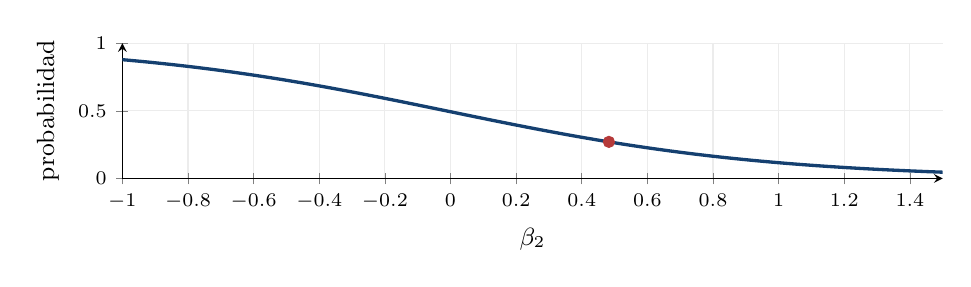
\begin{tikzpicture}
\begin{axis}[base,width=12cm,height=3.3cm,xmin=-1,xmax=1.5,ymin=0,ymax=1,xlabel={$\beta_2$},ylabel={probabilidad},ytick={0,.5,1}]
\addplot[azul,very thick,domain=-1:1.5]{1/(1+exp(-(-0.0276176263+(-2)*x)))};
\addplot[rojo,only marks,mark=*] coordinates {(0.4827511049,0.2702962922)};
\end{axis}
\end{tikzpicture}
\caption{Probabilidad de esta fila al variar \(\beta_2\), con \(\beta_1,\beta_3\) fijos; el punto marca el ajuste.}
\end{figure}

La varianza de una futura respuesta Bernoulli,
evaluada en el ajuste, es 0.19723621.
Describe variación de la respuesta, y no la variación
muestral de su probabilidad estimada calculada arriba.
\endgroup

\clearpage
\section{Predicción de la fila 2: abrir varianza y propagación}\label{logit111}
\begingroup\small
\setlength{\abovedisplayskip}{4pt}\setlength{\belowdisplayskip}{4pt}
La fila \(x_i\) se mantiene fija mientras los coeficientes
son estimados. Se sustituyen las tres coordenadas,
incluyendo el intercepto:
\[
\begin{aligned}
x_{2}\T\widehat\beta&=(1)(-0.02761763)+(-1)(0.48275110)+(1)(-0.09864310)\\&=-0.60901183,\\\widehat{\Prob}(Y_{2}=1\mid x_{2})&=\frac{e^{-0.60901183}}{1+e^{-0.60901183}}=0.35228465.\end{aligned}
\]

La varianza local del producto lineal desarrolla tres varianzas
y tres covarianzas, estas últimas multiplicadas por dos:
\[
\begin{aligned}
\widehat{\Var}(x_{2}\T\widehat\beta)&=\widehat{\Var}(\widehat\beta_1)+(-1)^2\widehat{\Var}(\widehat\beta_2)+(1)^2\widehat{\Var}(\widehat\beta_3)\\&\quad+2(-1)\widehat{\Cov}(\widehat\beta_1,\widehat\beta_2)+2(1)\widehat{\Cov}(\widehat\beta_1,\widehat\beta_3)\\&\quad+2(-1)(1)\widehat{\Cov}(\widehat\beta_2,\widehat\beta_3)\\&=(0.818232)+(0.149366)+(0.924437)\\&\quad+(0.207546)+(-1.105641)+(0.032151)\\&=1.02609172.\end{aligned}
\]

La derivada de la probabilidad respecto de los tres coeficientes
es el factor Bernoulli por la columna de datos:
\[
\frac{e^{-0.60901183}}{(1+e^{-0.60901183})^2}x_{2}\approx\begin{pmatrix}0.22818017\\-0.22818017\\0.22818017\end{pmatrix}.
\]

La propagación de primer orden multiplica la varianza del
producto lineal por el cuadrado de ese factor:
\[
\widehat{\Var}\bigl(\widehat{\Prob}(Y_{2}=1\mid x_{2})\bigr)\approx(0.22818017)^2(1.02609172)=0.05342469.
\]

El intervalo local de 95\% en el producto lineal,
transformado a probabilidad por ambos extremos, produce
\[
\begin{aligned}
x_{2}\T\beta:&\quad[-2.59438059,1.37635692],\\\Prob(Y_{2}=1\mid x_{2}):&\quad[0.06950095,0.79840527].\end{aligned}
\]
La curva decrece al mover esta pendiente, porque el dato $x_{i2}$ es negativo. El signo de la coordenada del dato se conserva en la derivada de la probabilidad.
\begin{figure}[H]\centering
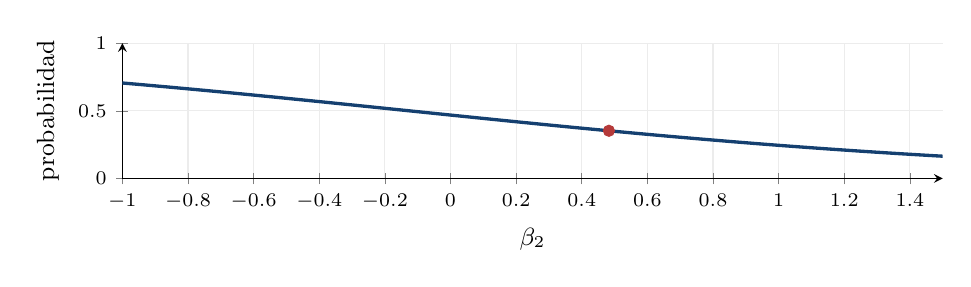
\begin{tikzpicture}
\begin{axis}[base,width=12cm,height=3.3cm,xmin=-1,xmax=1.5,ymin=0,ymax=1,xlabel={$\beta_2$},ylabel={probabilidad},ytick={0,.5,1}]
\addplot[azul,very thick,domain=-1:1.5]{1/(1+exp(-(-0.1262607283+(-1)*x)))};
\addplot[rojo,only marks,mark=*] coordinates {(0.4827511049,0.3522846451)};
\end{axis}
\end{tikzpicture}
\caption{Probabilidad de esta fila al variar \(\beta_2\), con \(\beta_1,\beta_3\) fijos; el punto marca el ajuste.}
\end{figure}

La varianza de una futura respuesta Bernoulli,
evaluada en el ajuste, es 0.22818017.
Describe variación de la respuesta, y no la variación
muestral de su probabilidad estimada calculada arriba.
\endgroup

\clearpage
\section{Predicción de la fila 3: abrir varianza y propagación}\label{logit112}
\begingroup\small
\setlength{\abovedisplayskip}{4pt}\setlength{\belowdisplayskip}{4pt}
La fila \(x_i\) se mantiene fija mientras los coeficientes
son estimados. Se sustituyen las tres coordenadas,
incluyendo el intercepto:
\[
\begin{aligned}
x_{3}\T\widehat\beta&=(1)(-0.02761763)+(0)(0.48275110)+(0)(-0.09864310)\\&=-0.02761763,\\\widehat{\Prob}(Y_{3}=1\mid x_{3})&=\frac{e^{-0.02761763}}{1+e^{-0.02761763}}=0.49309603.\end{aligned}
\]

La varianza local del producto lineal desarrolla tres varianzas
y tres covarianzas, estas últimas multiplicadas por dos:
\[
\begin{aligned}
\widehat{\Var}(x_{3}\T\widehat\beta)&=\widehat{\Var}(\widehat\beta_1)+(0)^2\widehat{\Var}(\widehat\beta_2)+(0)^2\widehat{\Var}(\widehat\beta_3)\\&\quad+2(0)\widehat{\Cov}(\widehat\beta_1,\widehat\beta_2)+2(0)\widehat{\Cov}(\widehat\beta_1,\widehat\beta_3)\\&\quad+2(0)(0)\widehat{\Cov}(\widehat\beta_2,\widehat\beta_3)\\&=(0.818232)+(0.000000)+(0.000000)\\&\quad+(-0.000000)+(-0.000000)+(-0.000000)\\&=0.81823241.\end{aligned}
\]

La derivada de la probabilidad respecto de los tres coeficientes
es el factor Bernoulli por la columna de datos:
\[
\frac{e^{-0.02761763}}{(1+e^{-0.02761763})^2}x_{3}\approx\begin{pmatrix}0.24995234\\0\\0\end{pmatrix}.
\]

La propagación de primer orden multiplica la varianza del
producto lineal por el cuadrado de ese factor:
\[
\widehat{\Var}\bigl(\widehat{\Prob}(Y_{3}=1\mid x_{3})\bigr)\approx(0.24995234)^2(0.81823241)=0.05112003.
\]

El intervalo local de 95\% en el producto lineal,
transformado a probabilidad por ambos extremos, produce
\[
\begin{aligned}
x_{3}\T\beta:&\quad[-1.80052657,1.74529131],\\\Prob(Y_{3}=1\mid x_{3}):&\quad[0.14178698,0.85135791].\end{aligned}
\]
La probabilidad es constante al mover esta pendiente, porque el dato $x_{i2}$ vale cero. La derivada respecto de $\beta_2$ es cero en toda la curva.
\begin{figure}[H]\centering
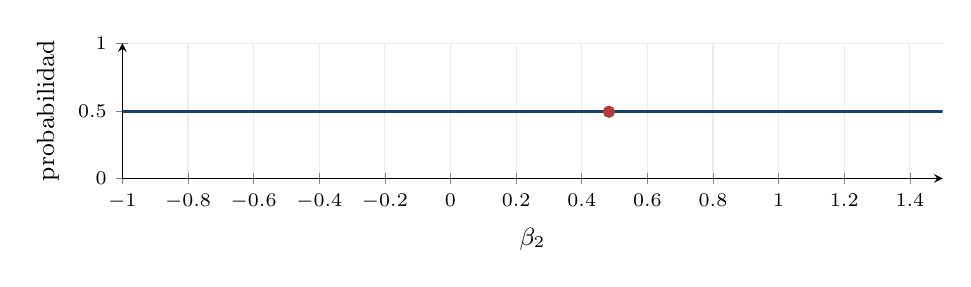
\begin{tikzpicture}
\begin{axis}[base,width=12cm,height=3.3cm,xmin=-1,xmax=1.5,ymin=0,ymax=1,xlabel={$\beta_2$},ylabel={probabilidad},ytick={0,.5,1}]
\addplot[azul,very thick,domain=-1:1.5]{1/(1+exp(-(-0.0276176263+(0)*x)))};
\addplot[rojo,only marks,mark=*] coordinates {(0.4827511049,0.4930960322)};
\end{axis}
\end{tikzpicture}
\caption{Probabilidad de esta fila al variar \(\beta_2\), con \(\beta_1,\beta_3\) fijos; el punto marca el ajuste.}
\end{figure}

La varianza de una futura respuesta Bernoulli,
evaluada en el ajuste, es 0.24995234.
Describe variación de la respuesta, y no la variación
muestral de su probabilidad estimada calculada arriba.
\endgroup

\clearpage
\section{Predicción de la fila 4: abrir varianza y propagación}\label{logit113}
\begingroup\small
\setlength{\abovedisplayskip}{4pt}\setlength{\belowdisplayskip}{4pt}
La fila \(x_i\) se mantiene fija mientras los coeficientes
son estimados. Se sustituyen las tres coordenadas,
incluyendo el intercepto:
\[
\begin{aligned}
x_{4}\T\widehat\beta&=(1)(-0.02761763)+(1)(0.48275110)+(1)(-0.09864310)\\&=0.35649038,\\\widehat{\Prob}(Y_{4}=1\mid x_{4})&=\frac{e^{0.35649038}}{1+e^{0.35649038}}=0.58819059.\end{aligned}
\]

La varianza local del producto lineal desarrolla tres varianzas
y tres covarianzas, estas últimas multiplicadas por dos:
\[
\begin{aligned}
\widehat{\Var}(x_{4}\T\widehat\beta)&=\widehat{\Var}(\widehat\beta_1)+(1)^2\widehat{\Var}(\widehat\beta_2)+(1)^2\widehat{\Var}(\widehat\beta_3)\\&\quad+2(1)\widehat{\Cov}(\widehat\beta_1,\widehat\beta_2)+2(1)\widehat{\Cov}(\widehat\beta_1,\widehat\beta_3)\\&\quad+2(1)(1)\widehat{\Cov}(\widehat\beta_2,\widehat\beta_3)\\&=(0.818232)+(0.149366)+(0.924437)\\&\quad+(-0.207546)+(-1.105641)+(-0.032151)\\&=0.54669762.\end{aligned}
\]

La derivada de la probabilidad respecto de los tres coeficientes
es el factor Bernoulli por la columna de datos:
\[
\frac{e^{0.35649038}}{(1+e^{0.35649038})^2}x_{4}\approx\begin{pmatrix}0.24222242\\0.24222242\\0.24222242\end{pmatrix}.
\]

La propagación de primer orden multiplica la varianza del
producto lineal por el cuadrado de ese factor:
\[
\widehat{\Var}\bigl(\widehat{\Prob}(Y_{4}=1\mid x_{4})\bigr)\approx(0.24222242)^2(0.54669762)=0.03207568.
\]

El intervalo local de 95\% en el producto lineal,
transformado a probabilidad por ambos extremos, produce
\[
\begin{aligned}
x_{4}\T\beta:&\quad[-1.09268746,1.80566821],\\\Prob(Y_{4}=1\mid x_{4}):&\quad[0.25111255,0.85883752].\end{aligned}
\]
La curva crece al mover esta pendiente, porque el dato $x_{i2}$ es positivo. Su magnitud controla la sensibilidad antes de multiplicar por el factor Bernoulli.
\begin{figure}[H]\centering
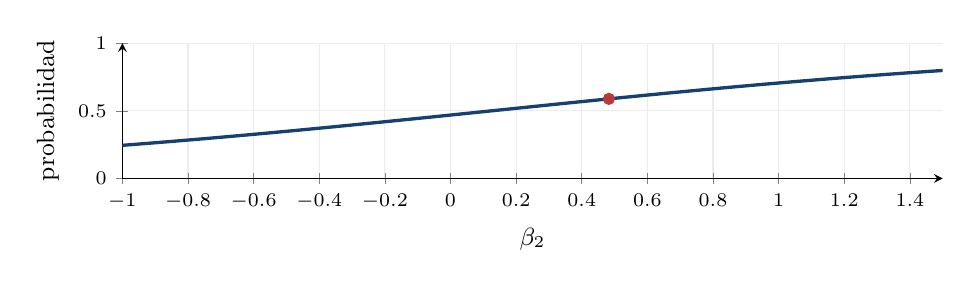
\begin{tikzpicture}
\begin{axis}[base,width=12cm,height=3.3cm,xmin=-1,xmax=1.5,ymin=0,ymax=1,xlabel={$\beta_2$},ylabel={probabilidad},ytick={0,.5,1}]
\addplot[azul,very thick,domain=-1:1.5]{1/(1+exp(-(-0.1262607283+(1)*x)))};
\addplot[rojo,only marks,mark=*] coordinates {(0.4827511049,0.5881905885)};
\end{axis}
\end{tikzpicture}
\caption{Probabilidad de esta fila al variar \(\beta_2\), con \(\beta_1,\beta_3\) fijos; el punto marca el ajuste.}
\end{figure}

La varianza de una futura respuesta Bernoulli,
evaluada en el ajuste, es 0.24222242.
Describe variación de la respuesta, y no la variación
muestral de su probabilidad estimada calculada arriba.
\endgroup

\clearpage
\section{Predicción de la fila 5: abrir varianza y propagación}\label{logit114}
\begingroup\small
\setlength{\abovedisplayskip}{4pt}\setlength{\belowdisplayskip}{4pt}
La fila \(x_i\) se mantiene fija mientras los coeficientes
son estimados. Se sustituyen las tres coordenadas,
incluyendo el intercepto:
\[
\begin{aligned}
x_{5}\T\widehat\beta&=(1)(-0.02761763)+(2)(0.48275110)+(0)(-0.09864310)\\&=0.93788458,\\\widehat{\Prob}(Y_{5}=1\mid x_{5})&=\frac{e^{0.93788458}}{1+e^{0.93788458}}=0.71867216.\end{aligned}
\]

La varianza local del producto lineal desarrolla tres varianzas
y tres covarianzas, estas últimas multiplicadas por dos:
\[
\begin{aligned}
\widehat{\Var}(x_{5}\T\widehat\beta)&=\widehat{\Var}(\widehat\beta_1)+(2)^2\widehat{\Var}(\widehat\beta_2)+(0)^2\widehat{\Var}(\widehat\beta_3)\\&\quad+2(2)\widehat{\Cov}(\widehat\beta_1,\widehat\beta_2)+2(0)\widehat{\Cov}(\widehat\beta_1,\widehat\beta_3)\\&\quad+2(2)(0)\widehat{\Cov}(\widehat\beta_2,\widehat\beta_3)\\&=(0.818232)+(0.597464)+(0.000000)\\&\quad+(-0.415093)+(-0.000000)+(-0.000000)\\&=1.00060340.\end{aligned}
\]

La derivada de la probabilidad respecto de los tres coeficientes
es el factor Bernoulli por la columna de datos:
\[
\frac{e^{0.93788458}}{(1+e^{0.93788458})^2}x_{5}\approx\begin{pmatrix}0.20218249\\0.40436498\\0\end{pmatrix}.
\]

La propagación de primer orden multiplica la varianza del
producto lineal por el cuadrado de ese factor:
\[
\widehat{\Var}\bigl(\widehat{\Prob}(Y_{5}=1\mid x_{5})\bigr)\approx(0.20218249)^2(1.00060340)=0.04090242.
\]

El intervalo local de 95\% en el producto lineal,
transformado a probabilidad por ambos extremos, produce
\[
\begin{aligned}
x_{5}\T\beta:&\quad[-1.02267063,2.89843980],\\\Prob(Y_{5}=1\mid x_{5}):&\quad[0.26450752,0.94776926].\end{aligned}
\]
La curva crece al mover esta pendiente, porque el dato $x_{i2}$ es positivo. Su magnitud controla la sensibilidad antes de multiplicar por el factor Bernoulli.
\begin{figure}[H]\centering
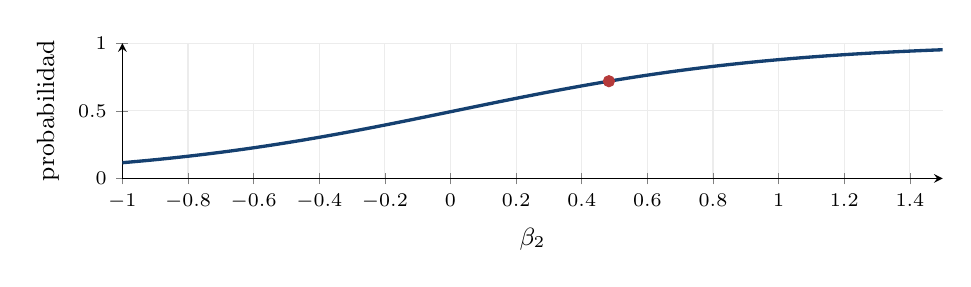
\begin{tikzpicture}
\begin{axis}[base,width=12cm,height=3.3cm,xmin=-1,xmax=1.5,ymin=0,ymax=1,xlabel={$\beta_2$},ylabel={probabilidad},ytick={0,.5,1}]
\addplot[azul,very thick,domain=-1:1.5]{1/(1+exp(-(-0.0276176263+(2)*x)))};
\addplot[rojo,only marks,mark=*] coordinates {(0.4827511049,0.7186721551)};
\end{axis}
\end{tikzpicture}
\caption{Probabilidad de esta fila al variar \(\beta_2\), con \(\beta_1,\beta_3\) fijos; el punto marca el ajuste.}
\end{figure}

La varianza de una futura respuesta Bernoulli,
evaluada en el ajuste, es 0.20218249.
Describe variación de la respuesta, y no la variación
muestral de su probabilidad estimada calculada arriba.
\endgroup

\clearpage
\section{Predicción de la fila 6: abrir varianza y propagación}\label{logit115}
\begingroup\small
\setlength{\abovedisplayskip}{4pt}\setlength{\belowdisplayskip}{4pt}
La fila \(x_i\) se mantiene fija mientras los coeficientes
son estimados. Se sustituyen las tres coordenadas,
incluyendo el intercepto:
\[
\begin{aligned}
x_{6}\T\widehat\beta&=(1)(-0.02761763)+(3)(0.48275110)+(1)(-0.09864310)\\&=1.32199259,\\\widehat{\Prob}(Y_{6}=1\mid x_{6})&=\frac{e^{1.32199259}}{1+e^{1.32199259}}=0.78951303.\end{aligned}
\]

La varianza local del producto lineal desarrolla tres varianzas
y tres covarianzas, estas últimas multiplicadas por dos:
\[
\begin{aligned}
\widehat{\Var}(x_{6}\T\widehat\beta)&=\widehat{\Var}(\widehat\beta_1)+(3)^2\widehat{\Var}(\widehat\beta_2)+(1)^2\widehat{\Var}(\widehat\beta_3)\\&\quad+2(3)\widehat{\Cov}(\widehat\beta_1,\widehat\beta_2)+2(1)\widehat{\Cov}(\widehat\beta_1,\widehat\beta_3)\\&\quad+2(3)(1)\widehat{\Cov}(\widehat\beta_2,\widehat\beta_3)\\&=(0.818232)+(1.344294)+(0.924437)\\&\quad+(-0.622639)+(-1.105641)+(-0.096452)\\&=1.26223144.\end{aligned}
\]

La derivada de la probabilidad respecto de los tres coeficientes
es el factor Bernoulli por la columna de datos:
\[
\frac{e^{1.32199259}}{(1+e^{1.32199259})^2}x_{6}\approx\begin{pmatrix}0.16618221\\0.49854662\\0.16618221\end{pmatrix}.
\]

La propagación de primer orden multiplica la varianza del
producto lineal por el cuadrado de ese factor:
\[
\widehat{\Var}\bigl(\widehat{\Prob}(Y_{6}=1\mid x_{6})\bigr)\approx(0.16618221)^2(1.26223144)=0.03485845.
\]

El intervalo local de 95\% en el producto lineal,
transformado a probabilidad por ambos extremos, produce
\[
\begin{aligned}
x_{6}\T\beta:&\quad[-0.88000880,3.52399397],\\\Prob(Y_{6}=1\mid x_{6}):&\quad[0.29317596,0.97136281].\end{aligned}
\]
La curva crece al mover esta pendiente, porque el dato $x_{i2}$ es positivo. Su magnitud controla la sensibilidad antes de multiplicar por el factor Bernoulli.
\begin{figure}[H]\centering
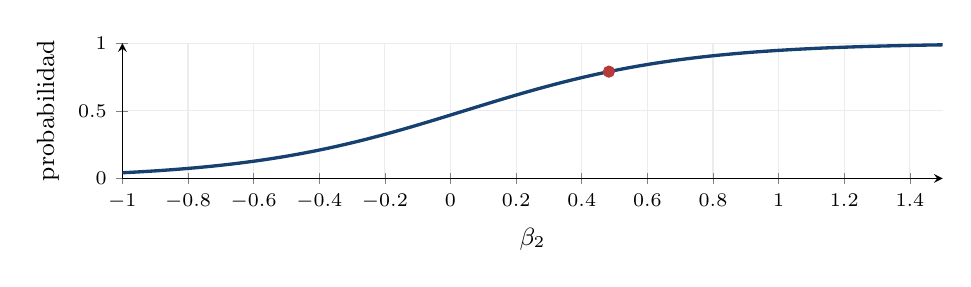
\begin{tikzpicture}
\begin{axis}[base,width=12cm,height=3.3cm,xmin=-1,xmax=1.5,ymin=0,ymax=1,xlabel={$\beta_2$},ylabel={probabilidad},ytick={0,.5,1}]
\addplot[azul,very thick,domain=-1:1.5]{1/(1+exp(-(-0.1262607283+(3)*x)))};
\addplot[rojo,only marks,mark=*] coordinates {(0.4827511049,0.7895130299)};
\end{axis}
\end{tikzpicture}
\caption{Probabilidad de esta fila al variar \(\beta_2\), con \(\beta_1,\beta_3\) fijos; el punto marca el ajuste.}
\end{figure}

La varianza de una futura respuesta Bernoulli,
evaluada en el ajuste, es 0.16618221.
Describe variación de la respuesta, y no la variación
muestral de su probabilidad estimada calculada arriba.
\endgroup

\clearpage
\section{Predicción de la fila 7: abrir varianza y propagación}\label{logit116}
\begingroup\small
\setlength{\abovedisplayskip}{4pt}\setlength{\belowdisplayskip}{4pt}
La fila \(x_i\) se mantiene fija mientras los coeficientes
son estimados. Se sustituyen las tres coordenadas,
incluyendo el intercepto:
\[
\begin{aligned}
x_{7}\T\widehat\beta&=(1)(-0.02761763)+(-1)(0.48275110)+(1)(-0.09864310)\\&=-0.60901183,\\\widehat{\Prob}(Y_{7}=1\mid x_{7})&=\frac{e^{-0.60901183}}{1+e^{-0.60901183}}=0.35228465.\end{aligned}
\]

La varianza local del producto lineal desarrolla tres varianzas
y tres covarianzas, estas últimas multiplicadas por dos:
\[
\begin{aligned}
\widehat{\Var}(x_{7}\T\widehat\beta)&=\widehat{\Var}(\widehat\beta_1)+(-1)^2\widehat{\Var}(\widehat\beta_2)+(1)^2\widehat{\Var}(\widehat\beta_3)\\&\quad+2(-1)\widehat{\Cov}(\widehat\beta_1,\widehat\beta_2)+2(1)\widehat{\Cov}(\widehat\beta_1,\widehat\beta_3)\\&\quad+2(-1)(1)\widehat{\Cov}(\widehat\beta_2,\widehat\beta_3)\\&=(0.818232)+(0.149366)+(0.924437)\\&\quad+(0.207546)+(-1.105641)+(0.032151)\\&=1.02609172.\end{aligned}
\]

La derivada de la probabilidad respecto de los tres coeficientes
es el factor Bernoulli por la columna de datos:
\[
\frac{e^{-0.60901183}}{(1+e^{-0.60901183})^2}x_{7}\approx\begin{pmatrix}0.22818017\\-0.22818017\\0.22818017\end{pmatrix}.
\]

La propagación de primer orden multiplica la varianza del
producto lineal por el cuadrado de ese factor:
\[
\widehat{\Var}\bigl(\widehat{\Prob}(Y_{7}=1\mid x_{7})\bigr)\approx(0.22818017)^2(1.02609172)=0.05342469.
\]

El intervalo local de 95\% en el producto lineal,
transformado a probabilidad por ambos extremos, produce
\[
\begin{aligned}
x_{7}\T\beta:&\quad[-2.59438059,1.37635692],\\\Prob(Y_{7}=1\mid x_{7}):&\quad[0.06950095,0.79840527].\end{aligned}
\]
La curva decrece al mover esta pendiente, porque el dato $x_{i2}$ es negativo. El signo de la coordenada del dato se conserva en la derivada de la probabilidad.
\begin{figure}[H]\centering
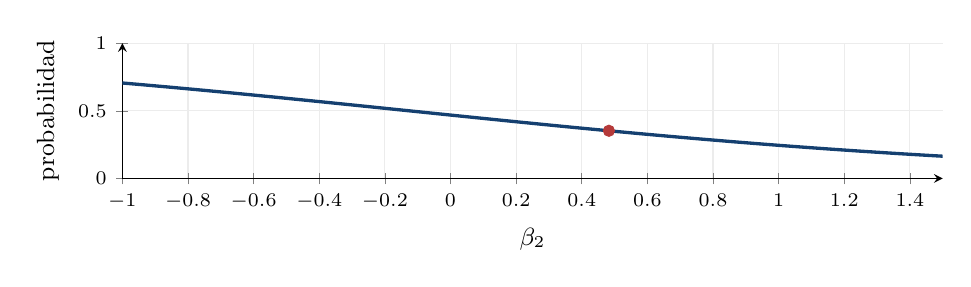
\begin{tikzpicture}
\begin{axis}[base,width=12cm,height=3.3cm,xmin=-1,xmax=1.5,ymin=0,ymax=1,xlabel={$\beta_2$},ylabel={probabilidad},ytick={0,.5,1}]
\addplot[azul,very thick,domain=-1:1.5]{1/(1+exp(-(-0.1262607283+(-1)*x)))};
\addplot[rojo,only marks,mark=*] coordinates {(0.4827511049,0.3522846451)};
\end{axis}
\end{tikzpicture}
\caption{Probabilidad de esta fila al variar \(\beta_2\), con \(\beta_1,\beta_3\) fijos; el punto marca el ajuste.}
\end{figure}

La varianza de una futura respuesta Bernoulli,
evaluada en el ajuste, es 0.22818017.
Describe variación de la respuesta, y no la variación
muestral de su probabilidad estimada calculada arriba.
\endgroup

\clearpage
\section{Predicción de la fila 8: abrir varianza y propagación}\label{logit117}
\begingroup\small
\setlength{\abovedisplayskip}{4pt}\setlength{\belowdisplayskip}{4pt}
La fila \(x_i\) se mantiene fija mientras los coeficientes
son estimados. Se sustituyen las tres coordenadas,
incluyendo el intercepto:
\[
\begin{aligned}
x_{8}\T\widehat\beta&=(1)(-0.02761763)+(0)(0.48275110)+(0)(-0.09864310)\\&=-0.02761763,\\\widehat{\Prob}(Y_{8}=1\mid x_{8})&=\frac{e^{-0.02761763}}{1+e^{-0.02761763}}=0.49309603.\end{aligned}
\]

La varianza local del producto lineal desarrolla tres varianzas
y tres covarianzas, estas últimas multiplicadas por dos:
\[
\begin{aligned}
\widehat{\Var}(x_{8}\T\widehat\beta)&=\widehat{\Var}(\widehat\beta_1)+(0)^2\widehat{\Var}(\widehat\beta_2)+(0)^2\widehat{\Var}(\widehat\beta_3)\\&\quad+2(0)\widehat{\Cov}(\widehat\beta_1,\widehat\beta_2)+2(0)\widehat{\Cov}(\widehat\beta_1,\widehat\beta_3)\\&\quad+2(0)(0)\widehat{\Cov}(\widehat\beta_2,\widehat\beta_3)\\&=(0.818232)+(0.000000)+(0.000000)\\&\quad+(-0.000000)+(-0.000000)+(-0.000000)\\&=0.81823241.\end{aligned}
\]

La derivada de la probabilidad respecto de los tres coeficientes
es el factor Bernoulli por la columna de datos:
\[
\frac{e^{-0.02761763}}{(1+e^{-0.02761763})^2}x_{8}\approx\begin{pmatrix}0.24995234\\0\\0\end{pmatrix}.
\]

La propagación de primer orden multiplica la varianza del
producto lineal por el cuadrado de ese factor:
\[
\widehat{\Var}\bigl(\widehat{\Prob}(Y_{8}=1\mid x_{8})\bigr)\approx(0.24995234)^2(0.81823241)=0.05112003.
\]

El intervalo local de 95\% en el producto lineal,
transformado a probabilidad por ambos extremos, produce
\[
\begin{aligned}
x_{8}\T\beta:&\quad[-1.80052657,1.74529131],\\\Prob(Y_{8}=1\mid x_{8}):&\quad[0.14178698,0.85135791].\end{aligned}
\]
La probabilidad es constante al mover esta pendiente, porque el dato $x_{i2}$ vale cero. La derivada respecto de $\beta_2$ es cero en toda la curva.
\begin{figure}[H]\centering
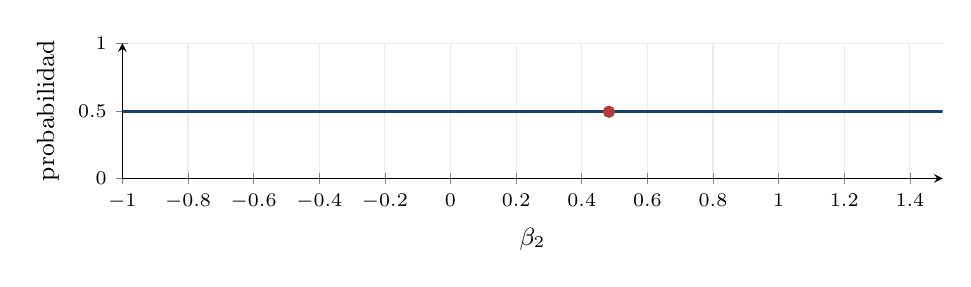
\begin{tikzpicture}
\begin{axis}[base,width=12cm,height=3.3cm,xmin=-1,xmax=1.5,ymin=0,ymax=1,xlabel={$\beta_2$},ylabel={probabilidad},ytick={0,.5,1}]
\addplot[azul,very thick,domain=-1:1.5]{1/(1+exp(-(-0.0276176263+(0)*x)))};
\addplot[rojo,only marks,mark=*] coordinates {(0.4827511049,0.4930960322)};
\end{axis}
\end{tikzpicture}
\caption{Probabilidad de esta fila al variar \(\beta_2\), con \(\beta_1,\beta_3\) fijos; el punto marca el ajuste.}
\end{figure}

La varianza de una futura respuesta Bernoulli,
evaluada en el ajuste, es 0.24995234.
Describe variación de la respuesta, y no la variación
muestral de su probabilidad estimada calculada arriba.
\endgroup

\clearpage
\section{Predicción de la fila 9: abrir varianza y propagación}\label{logit118}
\begingroup\small
\setlength{\abovedisplayskip}{4pt}\setlength{\belowdisplayskip}{4pt}
La fila \(x_i\) se mantiene fija mientras los coeficientes
son estimados. Se sustituyen las tres coordenadas,
incluyendo el intercepto:
\[
\begin{aligned}
x_{9}\T\widehat\beta&=(1)(-0.02761763)+(1)(0.48275110)+(2)(-0.09864310)\\&=0.25784727,\\\widehat{\Prob}(Y_{9}=1\mid x_{9})&=\frac{e^{0.25784727}}{1+e^{0.25784727}}=0.56410703.\end{aligned}
\]

La varianza local del producto lineal desarrolla tres varianzas
y tres covarianzas, estas últimas multiplicadas por dos:
\[
\begin{aligned}
\widehat{\Var}(x_{9}\T\widehat\beta)&=\widehat{\Var}(\widehat\beta_1)+(1)^2\widehat{\Var}(\widehat\beta_2)+(2)^2\widehat{\Var}(\widehat\beta_3)\\&\quad+2(1)\widehat{\Cov}(\widehat\beta_1,\widehat\beta_2)+2(2)\widehat{\Cov}(\widehat\beta_1,\widehat\beta_3)\\&\quad+2(1)(2)\widehat{\Cov}(\widehat\beta_2,\widehat\beta_3)\\&=(0.818232)+(0.149366)+(3.697750)\\&\quad+(-0.207546)+(-2.211282)+(-0.064301)\\&=2.18221830.\end{aligned}
\]

La derivada de la probabilidad respecto de los tres coeficientes
es el factor Bernoulli por la columna de datos:
\[
\frac{e^{0.25784727}}{(1+e^{0.25784727})^2}x_{9}\approx\begin{pmatrix}0.24589029\\0.24589029\\0.49178058\end{pmatrix}.
\]

La propagación de primer orden multiplica la varianza del
producto lineal por el cuadrado de ese factor:
\[
\widehat{\Var}\bigl(\widehat{\Prob}(Y_{9}=1\mid x_{9})\bigr)\approx(0.24589029)^2(2.18221830)=0.13194136.
\]

El intervalo local de 95\% en el producto lineal,
transformado a probabilidad por ambos extremos, produce
\[
\begin{aligned}
x_{9}\T\beta:&\quad[-2.63747684,3.15317139],\\\Prob(Y_{9}=1\mid x_{9}):&\quad[0.06676508,0.95903350].\end{aligned}
\]
La curva crece al mover esta pendiente, porque el dato $x_{i2}$ es positivo. Su magnitud controla la sensibilidad antes de multiplicar por el factor Bernoulli.
\begin{figure}[H]\centering
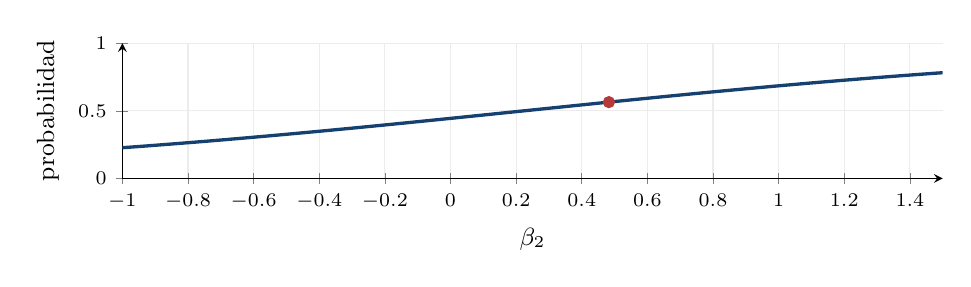
\begin{tikzpicture}
\begin{axis}[base,width=12cm,height=3.3cm,xmin=-1,xmax=1.5,ymin=0,ymax=1,xlabel={$\beta_2$},ylabel={probabilidad},ytick={0,.5,1}]
\addplot[azul,very thick,domain=-1:1.5]{1/(1+exp(-(-0.2249038303+(1)*x)))};
\addplot[rojo,only marks,mark=*] coordinates {(0.4827511049,0.5641070308)};
\end{axis}
\end{tikzpicture}
\caption{Probabilidad de esta fila al variar \(\beta_2\), con \(\beta_1,\beta_3\) fijos; el punto marca el ajuste.}
\end{figure}

La varianza de una futura respuesta Bernoulli,
evaluada en el ajuste, es 0.24589029.
Describe variación de la respuesta, y no la variación
muestral de su probabilidad estimada calculada arriba.
\endgroup

\clearpage
\section{Predicción de la fila 10: abrir varianza y propagación}\label{logit119}
\begingroup\small
\setlength{\abovedisplayskip}{4pt}\setlength{\belowdisplayskip}{4pt}
La fila \(x_i\) se mantiene fija mientras los coeficientes
son estimados. Se sustituyen las tres coordenadas,
incluyendo el intercepto:
\[
\begin{aligned}
x_{10}\T\widehat\beta&=(1)(-0.02761763)+(2)(0.48275110)+(0)(-0.09864310)\\&=0.93788458,\\\widehat{\Prob}(Y_{10}=1\mid x_{10})&=\frac{e^{0.93788458}}{1+e^{0.93788458}}=0.71867216.\end{aligned}
\]

La varianza local del producto lineal desarrolla tres varianzas
y tres covarianzas, estas últimas multiplicadas por dos:
\[
\begin{aligned}
\widehat{\Var}(x_{10}\T\widehat\beta)&=\widehat{\Var}(\widehat\beta_1)+(2)^2\widehat{\Var}(\widehat\beta_2)+(0)^2\widehat{\Var}(\widehat\beta_3)\\&\quad+2(2)\widehat{\Cov}(\widehat\beta_1,\widehat\beta_2)+2(0)\widehat{\Cov}(\widehat\beta_1,\widehat\beta_3)\\&\quad+2(2)(0)\widehat{\Cov}(\widehat\beta_2,\widehat\beta_3)\\&=(0.818232)+(0.597464)+(0.000000)\\&\quad+(-0.415093)+(-0.000000)+(-0.000000)\\&=1.00060340.\end{aligned}
\]

La derivada de la probabilidad respecto de los tres coeficientes
es el factor Bernoulli por la columna de datos:
\[
\frac{e^{0.93788458}}{(1+e^{0.93788458})^2}x_{10}\approx\begin{pmatrix}0.20218249\\0.40436498\\0\end{pmatrix}.
\]

La propagación de primer orden multiplica la varianza del
producto lineal por el cuadrado de ese factor:
\[
\widehat{\Var}\bigl(\widehat{\Prob}(Y_{10}=1\mid x_{10})\bigr)\approx(0.20218249)^2(1.00060340)=0.04090242.
\]

El intervalo local de 95\% en el producto lineal,
transformado a probabilidad por ambos extremos, produce
\[
\begin{aligned}
x_{10}\T\beta:&\quad[-1.02267063,2.89843980],\\\Prob(Y_{10}=1\mid x_{10}):&\quad[0.26450752,0.94776926].\end{aligned}
\]
La curva crece al mover esta pendiente, porque el dato $x_{i2}$ es positivo. Su magnitud controla la sensibilidad antes de multiplicar por el factor Bernoulli.
\begin{figure}[H]\centering
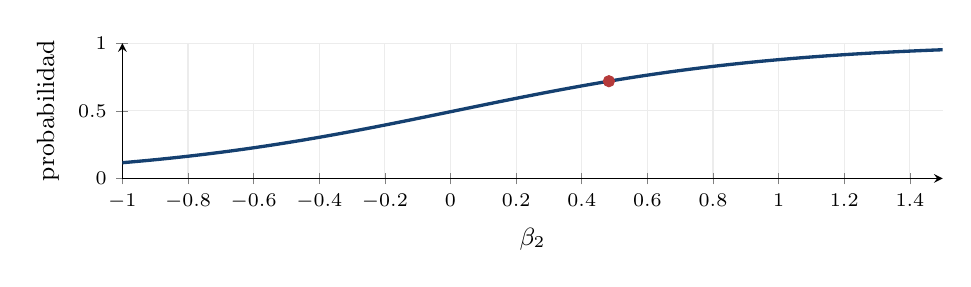
\begin{tikzpicture}
\begin{axis}[base,width=12cm,height=3.3cm,xmin=-1,xmax=1.5,ymin=0,ymax=1,xlabel={$\beta_2$},ylabel={probabilidad},ytick={0,.5,1}]
\addplot[azul,very thick,domain=-1:1.5]{1/(1+exp(-(-0.0276176263+(2)*x)))};
\addplot[rojo,only marks,mark=*] coordinates {(0.4827511049,0.7186721551)};
\end{axis}
\end{tikzpicture}
\caption{Probabilidad de esta fila al variar \(\beta_2\), con \(\beta_1,\beta_3\) fijos; el punto marca el ajuste.}
\end{figure}

La varianza de una futura respuesta Bernoulli,
evaluada en el ajuste, es 0.20218249.
Describe variación de la respuesta, y no la variación
muestral de su probabilidad estimada calculada arriba.
\endgroup

\clearpage
\section{Predicción de la fila 11: abrir varianza y propagación}\label{logit120}
\begingroup\small
\setlength{\abovedisplayskip}{4pt}\setlength{\belowdisplayskip}{4pt}
La fila \(x_i\) se mantiene fija mientras los coeficientes
son estimados. Se sustituyen las tres coordenadas,
incluyendo el intercepto:
\[
\begin{aligned}
x_{11}\T\widehat\beta&=(1)(-0.02761763)+(3)(0.48275110)+(1)(-0.09864310)\\&=1.32199259,\\\widehat{\Prob}(Y_{11}=1\mid x_{11})&=\frac{e^{1.32199259}}{1+e^{1.32199259}}=0.78951303.\end{aligned}
\]

La varianza local del producto lineal desarrolla tres varianzas
y tres covarianzas, estas últimas multiplicadas por dos:
\[
\begin{aligned}
\widehat{\Var}(x_{11}\T\widehat\beta)&=\widehat{\Var}(\widehat\beta_1)+(3)^2\widehat{\Var}(\widehat\beta_2)+(1)^2\widehat{\Var}(\widehat\beta_3)\\&\quad+2(3)\widehat{\Cov}(\widehat\beta_1,\widehat\beta_2)+2(1)\widehat{\Cov}(\widehat\beta_1,\widehat\beta_3)\\&\quad+2(3)(1)\widehat{\Cov}(\widehat\beta_2,\widehat\beta_3)\\&=(0.818232)+(1.344294)+(0.924437)\\&\quad+(-0.622639)+(-1.105641)+(-0.096452)\\&=1.26223144.\end{aligned}
\]

La derivada de la probabilidad respecto de los tres coeficientes
es el factor Bernoulli por la columna de datos:
\[
\frac{e^{1.32199259}}{(1+e^{1.32199259})^2}x_{11}\approx\begin{pmatrix}0.16618221\\0.49854662\\0.16618221\end{pmatrix}.
\]

La propagación de primer orden multiplica la varianza del
producto lineal por el cuadrado de ese factor:
\[
\widehat{\Var}\bigl(\widehat{\Prob}(Y_{11}=1\mid x_{11})\bigr)\approx(0.16618221)^2(1.26223144)=0.03485845.
\]

El intervalo local de 95\% en el producto lineal,
transformado a probabilidad por ambos extremos, produce
\[
\begin{aligned}
x_{11}\T\beta:&\quad[-0.88000880,3.52399397],\\\Prob(Y_{11}=1\mid x_{11}):&\quad[0.29317596,0.97136281].\end{aligned}
\]
La curva crece al mover esta pendiente, porque el dato $x_{i2}$ es positivo. Su magnitud controla la sensibilidad antes de multiplicar por el factor Bernoulli.
\begin{figure}[H]\centering
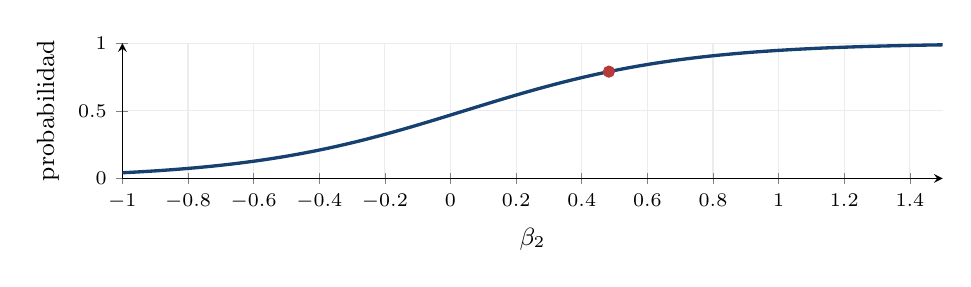
\begin{tikzpicture}
\begin{axis}[base,width=12cm,height=3.3cm,xmin=-1,xmax=1.5,ymin=0,ymax=1,xlabel={$\beta_2$},ylabel={probabilidad},ytick={0,.5,1}]
\addplot[azul,very thick,domain=-1:1.5]{1/(1+exp(-(-0.1262607283+(3)*x)))};
\addplot[rojo,only marks,mark=*] coordinates {(0.4827511049,0.7895130299)};
\end{axis}
\end{tikzpicture}
\caption{Probabilidad de esta fila al variar \(\beta_2\), con \(\beta_1,\beta_3\) fijos; el punto marca el ajuste.}
\end{figure}

La varianza de una futura respuesta Bernoulli,
evaluada en el ajuste, es 0.16618221.
Describe variación de la respuesta, y no la variación
muestral de su probabilidad estimada calculada arriba.
\endgroup

\clearpage
\section{Predicción de la fila 12: abrir varianza y propagación}\label{logit121}
\begingroup\small
\setlength{\abovedisplayskip}{4pt}\setlength{\belowdisplayskip}{4pt}
La fila \(x_i\) se mantiene fija mientras los coeficientes
son estimados. Se sustituyen las tres coordenadas,
incluyendo el intercepto:
\[
\begin{aligned}
x_{12}\T\widehat\beta&=(1)(-0.02761763)+(4)(0.48275110)+(0)(-0.09864310)\\&=1.90338679,\\\widehat{\Prob}(Y_{12}=1\mid x_{12})&=\frac{e^{1.90338679}}{1+e^{1.90338679}}=0.87027436.\end{aligned}
\]

La varianza local del producto lineal desarrolla tres varianzas
y tres covarianzas, estas últimas multiplicadas por dos:
\[
\begin{aligned}
\widehat{\Var}(x_{12}\T\widehat\beta)&=\widehat{\Var}(\widehat\beta_1)+(4)^2\widehat{\Var}(\widehat\beta_2)+(0)^2\widehat{\Var}(\widehat\beta_3)\\&\quad+2(4)\widehat{\Cov}(\widehat\beta_1,\widehat\beta_2)+2(0)\widehat{\Cov}(\widehat\beta_1,\widehat\beta_3)\\&\quad+2(4)(0)\widehat{\Cov}(\widehat\beta_2,\widehat\beta_3)\\&=(0.818232)+(2.389856)+(0.000000)\\&\quad+(-0.830186)+(-0.000000)+(-0.000000)\\&=2.37790231.\end{aligned}
\]

La derivada de la probabilidad respecto de los tres coeficientes
es el factor Bernoulli por la columna de datos:
\[
\frac{e^{1.90338679}}{(1+e^{1.90338679})^2}x_{12}\approx\begin{pmatrix}0.11289690\\0.45158758\\0\end{pmatrix}.
\]

La propagación de primer orden multiplica la varianza del
producto lineal por el cuadrado de ese factor:
\[
\widehat{\Var}\bigl(\widehat{\Prob}(Y_{12}=1\mid x_{12})\bigr)\approx(0.11289690)^2(2.37790231)=0.03030805.
\]

El intervalo local de 95\% en el producto lineal,
transformado a probabilidad por ambos extremos, produce
\[
\begin{aligned}
x_{12}\T\beta:&\quad[-1.11896557,4.92573915],\\\Prob(Y_{12}=1\mid x_{12}):&\quad[0.24620321,0.99279493].\end{aligned}
\]
La curva crece al mover esta pendiente, porque el dato $x_{i2}$ es positivo. Su magnitud controla la sensibilidad antes de multiplicar por el factor Bernoulli.
\begin{figure}[H]\centering
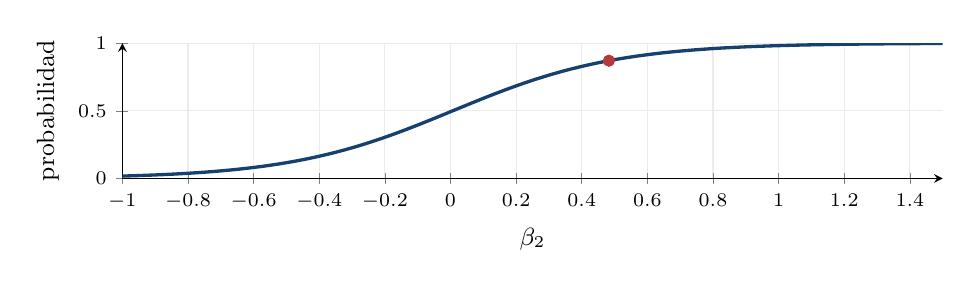
\begin{tikzpicture}
\begin{axis}[base,width=12cm,height=3.3cm,xmin=-1,xmax=1.5,ymin=0,ymax=1,xlabel={$\beta_2$},ylabel={probabilidad},ytick={0,.5,1}]
\addplot[azul,very thick,domain=-1:1.5]{1/(1+exp(-(-0.0276176263+(4)*x)))};
\addplot[rojo,only marks,mark=*] coordinates {(0.4827511049,0.8702743638)};
\end{axis}
\end{tikzpicture}
\caption{Probabilidad de esta fila al variar \(\beta_2\), con \(\beta_1,\beta_3\) fijos; el punto marca el ajuste.}
\end{figure}

La varianza de una futura respuesta Bernoulli,
evaluada en el ajuste, es 0.11289690.
Describe variación de la respuesta, y no la variación
muestral de su probabilidad estimada calculada arriba.
\endgroup

\clearpage
\section{Covarianza entre dos predicciones: conservar los nueve términos}\label{logit122}
Las filas 4 y 9 tienen datos \(x_4=(1,1,1)\T\) y
\(x_9=(1,1,2)\T\). Sus respuestas pueden ser independientes
dado el diseño y los parámetros verdaderos.
Sus probabilidades estimadas usan, sin embargo,
los mismos tres coeficientes aleatorios.
La covarianza local de los productos lineales es
\[
\widehat{\Cov}(x_4\T\widehat\beta,x_9\T\widehat\beta)
=x_4\T\widehat{\Cov}(\widehat\beta)x_9.
\]
Se multiplican las tres coordenadas de la primera fila
por las tres de la segunda y por cada entrada de la covarianza.
Aquí aparecen nueve términos, no solo tres:
\[
\begin{aligned}
&\widehat{\Var}(\widehat\beta_1)
+\widehat{\Cov}(\widehat\beta_1,\widehat\beta_2)
+2\widehat{\Cov}(\widehat\beta_1,\widehat\beta_3)\\
&+\widehat{\Cov}(\widehat\beta_2,\widehat\beta_1)
+\widehat{\Var}(\widehat\beta_2)
+2\widehat{\Cov}(\widehat\beta_2,\widehat\beta_3)\\
&+\widehat{\Cov}(\widehat\beta_3,\widehat\beta_1)
+\widehat{\Cov}(\widehat\beta_3,\widehat\beta_2)
+2\widehat{\Var}(\widehat\beta_3).
\end{aligned}
\]
Sustituir todas las entradas calculadas da
\[
0.9022392169.
\]

Para pasar a probabilidades, cada producto lineal se deriva
por separado. La covarianza aproximada queda
\[
\frac{e^{\widehat\beta_1+\widehat\beta_2+\widehat\beta_3}}
{(1+e^{\widehat\beta_1+\widehat\beta_2+\widehat\beta_3})^2}
\frac{e^{\widehat\beta_1+\widehat\beta_2+2\widehat\beta_3}}
{(1+e^{\widehat\beta_1+\widehat\beta_2+2\widehat\beta_3})^2}
\,x_4\T\widehat{\Cov}(\widehat\beta)x_9,
\]
cuyo valor es
\[
0.0537374948.
\]

No se ha afirmado covarianza no nula entre las respuestas
condicionadas en los parámetros verdaderos.
La dependencia calculada es la de dos funciones del mismo estimador.
Si se calculan doce predicciones, la matriz conjunta
es el Jacobiano de las doce probabilidades por la
covarianza de coeficientes por el Jacobiano transpuesto.
Su rango no supera tres en esta aproximación,
aunque contenga \(12\times12\) entradas.

La diferencia de dos predicciones tiene varianza
igual a la suma de sus varianzas menos dos veces
su covarianza. Compararlas como si fueran independientes
omitiría esa última cantidad.
Lo mismo ocurre al promediar probabilidades ajustadas:
se necesita sumar todas las covarianzas cruzadas,
no solo las doce varianzas diagonales.

\clearpage
\section{Experimento finito: cuatro filas y las dieciséis muestras posibles}\label{logit123}
Para calcular momentos de un estimador sin recurrir a un límite,
fijemos un diseño de cuatro filas y dos coeficientes:
\[
X=\begin{pmatrix}1&-1\\1&0\\1&1\\1&2\end{pmatrix},
\qquad
\beta_\star=\begin{pmatrix}0\\\log2\end{pmatrix}.
\]
El intercepto verdadero es cero.
Las probabilidades verdaderas se calculan usando cada fila:
\[
\begin{aligned}
\Prob(Y_1=1\mid X)&=\frac{e^{-\log2}}{1+e^{-\log2}}=\frac13,\\
\Prob(Y_2=1\mid X)&=\frac{e^0}{1+e^0}=\frac12,\\
\Prob(Y_3=1\mid X)&=\frac{e^{\log2}}{1+e^{\log2}}=\frac23,\\
\Prob(Y_4=1\mid X)&=\frac{e^{2\log2}}{1+e^{2\log2}}=\frac45.
\end{aligned}
\]
Condicionalmente en el diseño, las cuatro respuestas son
independientes. Hay \(2^4=16\) vectores posibles,
desde \((0,0,0,0)\T\) hasta \((1,1,1,1)\T\).
Su probabilidad se obtiene multiplicando cuatro factores:
\[
\Prob(Y=y\mid X)=
\left(\tfrac13\right)^{y_1}\left(\tfrac23\right)^{1-y_1}
\left(\tfrac12\right)^{y_2}\left(\tfrac12\right)^{1-y_2}
\left(\tfrac23\right)^{y_3}\left(\tfrac13\right)^{1-y_3}
\left(\tfrac45\right)^{y_4}\left(\tfrac15\right)^{1-y_4}.
\]
Por ejemplo, el vector de cuatro ceros tiene probabilidad
\((2/3)(1/2)(1/3)(1/5)=1/45\).
El de cuatro unos tiene probabilidad
\((1/3)(1/2)(2/3)(4/5)=4/45\).
Ninguno tiene probabilidad cero.

En esas dos muestras, el máximo ordinario no es finito.
Por eso no podemos calcular una covarianza finita
del estimador ordinario sobre estas dieciséis muestras.
Estudiaremos en cambio el estimador penalizado de
intensidad uno, incluyendo intercepto y pendiente:
\[
\widehat\beta_1,\widehat\beta_2
=\argmax_{\beta_1,\beta_2}
\left\{\sum_{i=1}^4
[y_i(\beta_1+x_{i2}\beta_2)-\log(1+e^{\beta_1+x_{i2}\beta_2})]
-\frac12(\beta_1^2+\beta_2^2)\right\}.
\]
Su existencia, unicidad y acotación ya se demostraron.
Cada una de las dieciséis muestras tiene una solución finita.

Las sumas de esperanza y covarianza serán identidades finitas,
sin aproximación normal y sin simulación Monte Carlo.
Los valores de las raíces y los momentos impresos son
aproximaciones numéricas de esas identidades.
Las probabilidades de las muestras sí son fracciones exactas.

\clearpage
\section{Ecuaciones del experimento penalizado: todos los exponenciales abiertos}\label{logit124}
La contribución de penalización \(-(\beta_1^2+\beta_2^2)/2\)
tiene derivadas \(-\beta_1\) y \(-\beta_2\).
Los cuatro productos lineales son
\(\beta_1-\beta_2\), \(\beta_1\),
\(\beta_1+\beta_2\), \(\beta_1+2\beta_2\).
Por ello las ecuaciones de las dos coordenadas son
\[
\begin{aligned}
0={}&y_1+y_2+y_3+y_4-\beta_1\\
&-\frac{e^{\beta_1-\beta_2}}{1+e^{\beta_1-\beta_2}}
-\frac{e^{\beta_1}}{1+e^{\beta_1}}\\
&-\frac{e^{\beta_1+\beta_2}}{1+e^{\beta_1+\beta_2}}
-\frac{e^{\beta_1+2\beta_2}}{1+e^{\beta_1+2\beta_2}},\\[3pt]
0={}&-y_1+y_3+2y_4-\beta_2
+\frac{e^{\beta_1-\beta_2}}{1+e^{\beta_1-\beta_2}}\\
&-\frac{e^{\beta_1+\beta_2}}{1+e^{\beta_1+\beta_2}}
-2\frac{e^{\beta_1+2\beta_2}}{1+e^{\beta_1+2\beta_2}}.
\end{aligned}
\]
La fila \(x_{22}=0\) no contribuye a la segunda coordenada,
pero sí contribuye al intercepto.
La fila \(x_{12}=-1\) explica el signo positivo de su
probabilidad en esa segunda ecuación.

La curvatura positiva penalizada se obtiene agregando
\(I_2\) a las contribuciones de las cuatro filas:
\[
I_2+
\frac{e^{\beta_1-\beta_2}}{(1+e^{\beta_1-\beta_2})^2}
\begin{pmatrix}1&-1\\-1&1\end{pmatrix}
+\frac{e^{\beta_1}}{(1+e^{\beta_1})^2}
\begin{pmatrix}1&0\\0&0\end{pmatrix}
\]
\[
+\frac{e^{\beta_1+\beta_2}}{(1+e^{\beta_1+\beta_2})^2}
\begin{pmatrix}1&1\\1&1\end{pmatrix}
+\frac{e^{\beta_1+2\beta_2}}{(1+e^{\beta_1+2\beta_2})^2}
\begin{pmatrix}1&2\\2&4\end{pmatrix}.
\]
Cada autovalor es al menos uno.
No hay pérdida de inversibilidad al acercar
una probabilidad al cero o al uno.

En el inicio \(\beta=(0,0)\T\), la matriz es
\[
I_2+\frac14\begin{pmatrix}4&2\\2&6\end{pmatrix}
=\begin{pmatrix}2&1/2\\1/2&5/2\end{pmatrix}.
\]
El gradiente es
\[
\begin{pmatrix}
y_1+y_2+y_3+y_4-2\\-y_1+y_3+2y_4-1
\end{pmatrix}.
\]
Su solución de Newton depende de las respuestas,
pero la primera curvatura es común a todas las muestras.
Después del primer paso, las curvaturas también cambian
entre configuraciones porque cambian los coeficientes.

\clearpage
\section{Muestra 0000: raíz penalizada y aporte a los momentos}\label{logit125}
\begingroup\small
\setlength{\abovedisplayskip}{4pt}\setlength{\belowdisplayskip}{4pt}
Se mantienen las cuatro filas del experimento y se observa
la siguiente configuración de respuestas:
\[
y=\begin{pmatrix}0\\0\\0\\0\end{pmatrix},\quad \Prob(Y=y\mid X)=\frac{2}{3}\cdot\frac{1}{2}\cdot\frac{1}{3}\cdot\frac{1}{5}=\frac{1}{45}.
\]

El conteo de unos y el producto con el segundo regresor son
\[
\sum_{i=1}^4 y_i=0,\qquad\sum_{i=1}^4x_{i2}y_i=(-1)(0)+0(0)+1(0)+2(0)=0.
\]

En las ecuaciones abiertas de la unidad anterior se sustituyen
estos dos resultados. En el inicio, el sistema produce
\[
\begin{pmatrix}2&1/2\\1/2&5/2\end{pmatrix}\Delta^{(0)}=\begin{pmatrix}-2\\-1\end{pmatrix},\qquad\Delta^{(0)}=\begin{pmatrix}-0.94736842\\-0.21052632\end{pmatrix}.
\]

Se recalculan probabilidades y curvatura hasta resolver
ambas ecuaciones. La solución y el objetivo penalizado son
\[
\widehat\beta(y)\approx\begin{pmatrix}-0.99575846\\-0.25896422\end{pmatrix},\qquad \ell(\widehat\beta(y))-\tfrac12\|\widehat\beta(y)\|_2^2\approx-1.6846392328.
\]

La sustitución final en cada fila permite verificar
los dos gradientes, incluyendo el término de penalización.
\begin{center}\scriptsize
\begin{tabular}{rrrrrrr}\toprule
\(i\)&\(x_{i2}\)&\(y_i\)&\(\widehat\beta_1+x_{i2}\widehat\beta_2\)&probabilidad&discrepancia&varianza\\\midrule
1&-1&0&-0.73679424&0.32370555&-0.32370555&0.21892027\\
2&0&0&-0.99575846&0.26977618&-0.26977618&0.19699699\\
3&1&0&-1.25472268&0.22188369&-0.22188369&0.17265132\\
4&2&0&-1.51368689&0.18039304&-0.18039304&0.14785139\\
\\\bottomrule\end{tabular}\end{center}
La suma de discrepancias coincide con \(\widehat\beta_1\).
La suma de \(x_{i2}\) por discrepancia coincide con
\(\widehat\beta_2\). Los residuos de ambas ecuaciones
tienen valor absoluto menor que \(10^{-10}\).

La curvatura positiva penalizada en la raíz es
\[
\begin{pmatrix}1.73641997&0.24943383\\0.24943383&1.98297715\end{pmatrix}.
\]

La muestra aporta a la esperanza su probabilidad
multiplicada por el vector de coeficientes:
\[
\frac{1}{45}\,\begin{pmatrix}-0.99575846\\-0.25896422\end{pmatrix}=\begin{pmatrix}-0.02212797\\-0.00575476\end{pmatrix}.
\]

A los segundos momentos aporta esa misma probabilidad
por todos los productos de coeficientes, incluidos los cruzados:
\[
\frac{1}{45}\,\begin{pmatrix}0.99153491&0.25786581\\0.25786581&0.06706247\end{pmatrix}.
\]

\begin{figure}[H]\centering
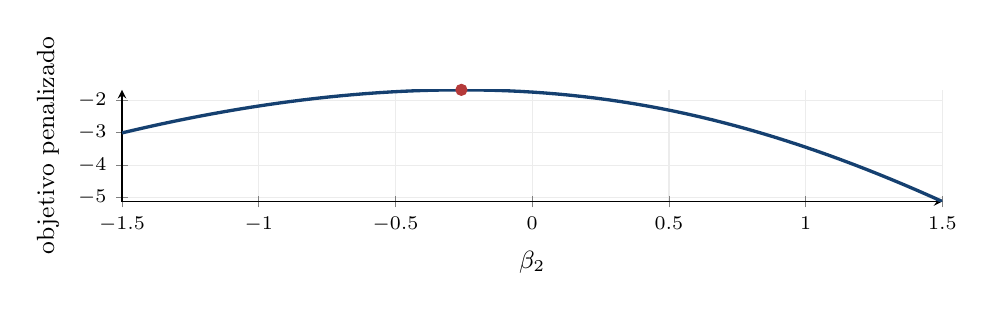
\begin{tikzpicture}
\begin{axis}[base,width=12cm,height=3cm,xmin=-1.5,xmax=1.5,xlabel={$\beta_2$},ylabel={objetivo penalizado}]
\addplot[azul,very thick] coordinates {(-1.50000,-3.00932942) (-1.45312,-2.91657169) (-1.40625,-2.82686429) (-1.35938,-2.74023496) (-1.31250,-2.65671256) (-1.26562,-2.57632717) (-1.21875,-2.49911018) (-1.17188,-2.42509441) (-1.12500,-2.35431425) (-1.07812,-2.28680570) (-1.03125,-2.22260660) (-0.98438,-2.16175667) (-0.93750,-2.10429769) (-0.89062,-2.05027362) (-0.84375,-1.99973071) (-0.79688,-1.95271766) (-0.75000,-1.90928567) (-0.70312,-1.86948862) (-0.65625,-1.83338307) (-0.60938,-1.80102838) (-0.56250,-1.77248668) (-0.51562,-1.74782291) (-0.46875,-1.72710475) (-0.42188,-1.71040251) (-0.37500,-1.69778899) (-0.32812,-1.68933922) (-0.28125,-1.68513023) (-0.23438,-1.68524064) (-0.18750,-1.68975021) (-0.14062,-1.69873934) (-0.09375,-1.71228845) (-0.04688,-1.73047729) (0.00000,-1.75338419) (0.04688,-1.78108522) (0.09375,-1.81365334) (0.14062,-1.85115748) (0.18750,-1.89366162) (0.23438,-1.94122387) (0.28125,-1.99389560) (0.32812,-2.05172062) (0.37500,-2.11473443) (0.42188,-2.18296360) (0.46875,-2.25642526) (0.51562,-2.33512675) (0.56250,-2.41906543) (0.60938,-2.50822864) (0.65625,-2.60259385) (0.70312,-2.70212899) (0.75000,-2.80679284) (0.79688,-2.91653568) (0.84375,-3.03129999) (0.89062,-3.15102120) (0.93750,-3.27562861) (0.98438,-3.40504627) (1.03125,-3.53919391) (1.07812,-3.67798782) (1.12500,-3.82134182) (1.17188,-3.96916799) (1.21875,-4.12137758) (1.26562,-4.27788162) (1.31250,-4.43859165) (1.35938,-4.60342021) (1.40625,-4.77228139) (1.45312,-4.94509120) (1.50000,-5.12176793)};\addplot[rojo,only marks,mark=*] coordinates {(-0.25896422,-1.68463923)};
\end{axis}
\end{tikzpicture}
\caption{Objetivo penalizado al mover \(\beta_2\), fijando \(\beta_1\) en su solución para esta muestra.}
\end{figure}

La suma de los dieciséis aportes forma los momentos finitos.
Una muestra con baja probabilidad tiene menos peso,
aunque sus coeficientes puedan ser de magnitud grande.
La gráfica es un corte de la función de dos variables;
mantiene fijo el intercepto, y no es un perfil reoptimizado.
\endgroup

\clearpage
\section{Muestra 0001: raíz penalizada y aporte a los momentos}\label{logit126}
\begingroup\small
\setlength{\abovedisplayskip}{4pt}\setlength{\belowdisplayskip}{4pt}
Se mantienen las cuatro filas del experimento y se observa
la siguiente configuración de respuestas:
\[
y=\begin{pmatrix}0\\0\\0\\1\end{pmatrix},\quad \Prob(Y=y\mid X)=\frac{2}{3}\cdot\frac{1}{2}\cdot\frac{1}{3}\cdot\frac{4}{5}=\frac{4}{45}.
\]

El conteo de unos y el producto con el segundo regresor son
\[
\sum_{i=1}^4 y_i=1,\qquad\sum_{i=1}^4x_{i2}y_i=(-1)(0)+0(0)+1(0)+2(1)=2.
\]

En las ecuaciones abiertas de la unidad anterior se sustituyen
estos dos resultados. En el inicio, el sistema produce
\[
\begin{pmatrix}2&1/2\\1/2&5/2\end{pmatrix}\Delta^{(0)}=\begin{pmatrix}-1\\1\end{pmatrix},\qquad\Delta^{(0)}=\begin{pmatrix}-0.63157895\\0.52631579\end{pmatrix}.
\]

Se recalculan probabilidades y curvatura hasta resolver
ambas ecuaciones. La solución y el objetivo penalizado son
\[
\widehat\beta(y)\approx\begin{pmatrix}-0.65380458\\0.54464644\end{pmatrix},\qquad \ell(\widehat\beta(y))-\tfrac12\|\widehat\beta(y)\|_2^2\approx-2.1834244560.
\]

La sustitución final en cada fila permite verificar
los dos gradientes, incluyendo el término de penalización.
\begin{center}\scriptsize
\begin{tabular}{rrrrrrr}\toprule
\(i\)&\(x_{i2}\)&\(y_i\)&\(\widehat\beta_1+x_{i2}\widehat\beta_2\)&probabilidad&discrepancia&varianza\\\midrule
1&-1&0&-1.19845101&0.23175089&-0.23175089&0.17804241\\
2&0&0&-0.65380458&0.34213270&-0.34213270&0.22507791\\
3&1&0&-0.10915814&0.47273753&-0.47273753&0.24925676\\
4&2&1&0.43548830&0.60718346&0.39281654&0.23851171\\
\\\bottomrule\end{tabular}\end{center}
La suma de discrepancias coincide con \(\widehat\beta_1\).
La suma de \(x_{i2}\) por discrepancia coincide con
\(\widehat\beta_2\). Los residuos de ambas ecuaciones
tienen valor absoluto menor que \(10^{-10}\).

La curvatura positiva penalizada en la raíz es
\[
\begin{pmatrix}1.89088879&0.54823776\\0.54823776&2.38134600\end{pmatrix}.
\]

La muestra aporta a la esperanza su probabilidad
multiplicada por el vector de coeficientes:
\[
\frac{4}{45}\,\begin{pmatrix}-0.65380458\\0.54464644\end{pmatrix}=\begin{pmatrix}-0.05811596\\0.04841302\end{pmatrix}.
\]

A los segundos momentos aporta esa misma probabilidad
por todos los productos de coeficientes, incluidos los cruzados:
\[
\frac{4}{45}\,\begin{pmatrix}0.42746042&-0.35609233\\-0.35609233&0.29663974\end{pmatrix}.
\]

\begin{figure}[H]\centering
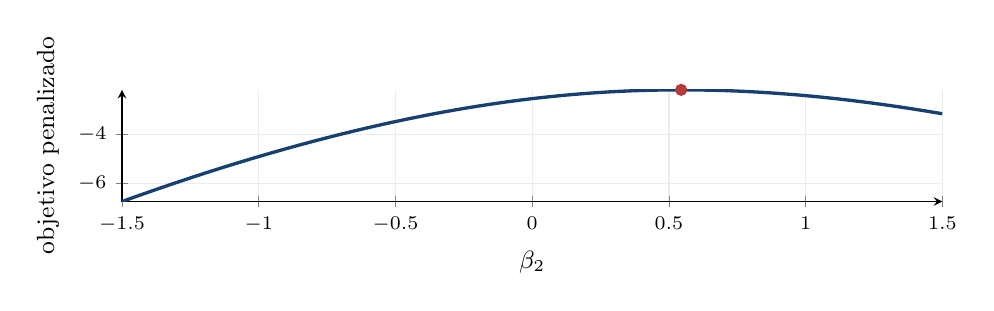
\begin{tikzpicture}
\begin{axis}[base,width=12cm,height=3cm,xmin=-1.5,xmax=1.5,xlabel={$\beta_2$},ylabel={objetivo penalizado}]
\addplot[azul,very thick] coordinates {(-1.50000,-6.74983929) (-1.45312,-6.56176108) (-1.40625,-6.37679912) (-1.35938,-6.19499136) (-1.31250,-6.01637746) (-1.26562,-5.84099896) (-1.21875,-5.66889931) (-1.17188,-5.50012402) (-1.12500,-5.33472075) (-1.07812,-5.17273940) (-1.03125,-5.01423224) (-0.98438,-4.85925399) (-0.93750,-4.70786190) (-0.89062,-4.56011581) (-0.84375,-4.41607825) (-0.79688,-4.27581443) (-0.75000,-4.13939226) (-0.70312,-4.00688233) (-0.65625,-3.87835782) (-0.60938,-3.75389443) (-0.56250,-3.63357017) (-0.51562,-3.51746515) (-0.46875,-3.40566129) (-0.42188,-3.29824195) (-0.37500,-3.19529150) (-0.32812,-3.09689481) (-0.28125,-3.00313660) (-0.23438,-2.91410084) (-0.18750,-2.82986995) (-0.14062,-2.75052399) (-0.09375,-2.67613985) (-0.04688,-2.60679026) (0.00000,-2.54254293) (0.04688,-2.48345964) (0.09375,-2.42959529) (0.14062,-2.38099712) (0.18750,-2.33770388) (0.23438,-2.29974526) (0.28125,-2.26714126) (0.32812,-2.23990184) (0.37500,-2.21802670) (0.42188,-2.20150515) (0.46875,-2.19031630) (0.51562,-2.18442924) (0.56250,-2.18380351) (0.60938,-2.18838966) (0.65625,-2.19812993) (0.70312,-2.21295907) (0.75000,-2.23280514) (0.79688,-2.25759052) (0.84375,-2.28723277) (0.89062,-2.32164562) (0.93750,-2.36073986) (0.98438,-2.40442426) (1.03125,-2.45260635) (1.07812,-2.50519326) (1.12500,-2.56209231) (1.17188,-2.62321171) (1.21875,-2.68846104) (1.26562,-2.75775173) (1.31250,-2.83099740) (1.35938,-2.90811421) (1.40625,-2.98902104) (1.45312,-3.07363971) (1.50000,-3.16189508)};\addplot[rojo,only marks,mark=*] coordinates {(0.54464644,-2.18342446)};
\end{axis}
\end{tikzpicture}
\caption{Objetivo penalizado al mover \(\beta_2\), fijando \(\beta_1\) en su solución para esta muestra.}
\end{figure}

La suma de los dieciséis aportes forma los momentos finitos.
Una muestra con baja probabilidad tiene menos peso,
aunque sus coeficientes puedan ser de magnitud grande.
La gráfica es un corte de la función de dos variables;
mantiene fijo el intercepto, y no es un perfil reoptimizado.
\endgroup

\clearpage
\section{Muestra 0010: raíz penalizada y aporte a los momentos}\label{logit127}
\begingroup\small
\setlength{\abovedisplayskip}{4pt}\setlength{\belowdisplayskip}{4pt}
Se mantienen las cuatro filas del experimento y se observa
la siguiente configuración de respuestas:
\[
y=\begin{pmatrix}0\\0\\1\\0\end{pmatrix},\quad \Prob(Y=y\mid X)=\frac{2}{3}\cdot\frac{1}{2}\cdot\frac{2}{3}\cdot\frac{1}{5}=\frac{2}{45}.
\]

El conteo de unos y el producto con el segundo regresor son
\[
\sum_{i=1}^4 y_i=1,\qquad\sum_{i=1}^4x_{i2}y_i=(-1)(0)+0(0)+1(1)+2(0)=1.
\]

En las ecuaciones abiertas de la unidad anterior se sustituyen
estos dos resultados. En el inicio, el sistema produce
\[
\begin{pmatrix}2&1/2\\1/2&5/2\end{pmatrix}\Delta^{(0)}=\begin{pmatrix}-1\\0\end{pmatrix},\qquad\Delta^{(0)}=\begin{pmatrix}-0.52631579\\0.10526316\end{pmatrix}.
\]

Se recalculan probabilidades y curvatura hasta resolver
ambas ecuaciones. La solución y el objetivo penalizado son
\[
\widehat\beta(y)\approx\begin{pmatrix}-0.53209600\\0.10735785\end{pmatrix},\qquad \ell(\widehat\beta(y))-\tfrac12\|\widehat\beta(y)\|_2^2\approx-2.5079860843.
\]

La sustitución final en cada fila permite verificar
los dos gradientes, incluyendo el término de penalización.
\begin{center}\scriptsize
\begin{tabular}{rrrrrrr}\toprule
\(i\)&\(x_{i2}\)&\(y_i\)&\(\widehat\beta_1+x_{i2}\widehat\beta_2\)&probabilidad&discrepancia&varianza\\\midrule
1&-1&0&-0.63945385&0.34537001&-0.34537001&0.22608957\\
2&0&0&-0.53209600&0.37002816&-0.37002816&0.23310732\\
3&1&1&-0.42473815&0.39538351&0.60461649&0.23905539\\
4&2&0&-0.31738030&0.42131432&-0.42131432&0.24380856\\
\\\bottomrule\end{tabular}\end{center}
La suma de discrepancias coincide con \(\widehat\beta_1\).
La suma de \(x_{i2}\) por discrepancia coincide con
\(\widehat\beta_2\). Los residuos de ambas ecuaciones
tienen valor absoluto menor que \(10^{-10}\).

La curvatura positiva penalizada en la raíz es
\[
\begin{pmatrix}1.94206084&0.50058295\\0.50058295&2.44037921\end{pmatrix}.
\]

La muestra aporta a la esperanza su probabilidad
multiplicada por el vector de coeficientes:
\[
\frac{2}{45}\,\begin{pmatrix}-0.53209600\\0.10735785\end{pmatrix}=\begin{pmatrix}-0.02364871\\0.00477146\end{pmatrix}.
\]

A los segundos momentos aporta esa misma probabilidad
por todos los productos de coeficientes, incluidos los cruzados:
\[
\frac{2}{45}\,\begin{pmatrix}0.28312615&-0.05712468\\-0.05712468&0.01152571\end{pmatrix}.
\]

\begin{figure}[H]\centering
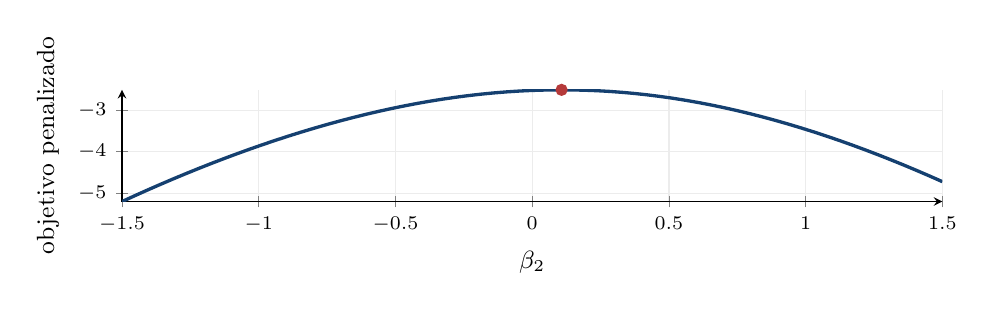
\begin{tikzpicture}
\begin{axis}[base,width=12cm,height=3cm,xmin=-1.5,xmax=1.5,xlabel={$\beta_2$},ylabel={objetivo penalizado}]
\addplot[azul,very thick] coordinates {(-1.50000,-5.20261848) (-1.45312,-5.06111410) (-1.40625,-4.92275295) (-1.35938,-4.78757661) (-1.31250,-4.65562864) (-1.26562,-4.52695468) (-1.21875,-4.40160252) (-1.17188,-4.27962226) (-1.12500,-4.16106635) (-1.07812,-4.04598971) (-1.03125,-3.93444984) (-0.98438,-3.82650681) (-0.93750,-3.72222343) (-0.89062,-3.62166521) (-0.84375,-3.52490040) (-0.79688,-3.43199998) (-0.75000,-3.34303763) (-0.70312,-3.25808959) (-0.65625,-3.17723456) (-0.60938,-3.10055350) (-0.56250,-3.02812935) (-0.51562,-2.96004674) (-0.46875,-2.89639156) (-0.42188,-2.83725051) (-0.37500,-2.78271052) (-0.32812,-2.73285815) (-0.28125,-2.68777887) (-0.23438,-2.64755627) (-0.18750,-2.61227125) (-0.14062,-2.58200111) (-0.09375,-2.55681862) (-0.04688,-2.53679116) (0.00000,-2.52197973) (0.04688,-2.51243807) (0.09375,-2.50821191) (0.14062,-2.50933813) (0.18750,-2.51584422) (0.23438,-2.52774773) (0.28125,-2.54505594) (0.32812,-2.56776569) (0.37500,-2.59586333) (0.42188,-2.62932492) (0.46875,-2.66811651) (0.51562,-2.71219462) (0.56250,-2.76150689) (0.60938,-2.81599274) (0.65625,-2.87558427) (0.70312,-2.94020710) (0.75000,-3.00978131) (0.79688,-3.08422241) (0.84375,-3.16344228) (0.89062,-3.24735007) (0.93750,-3.33585310) (0.98438,-3.42885770) (1.03125,-3.52626988) (1.07812,-3.62799611) (1.12500,-3.73394381) (1.17188,-3.84402196) (1.21875,-3.95814146) (1.26562,-4.07621553) (1.31250,-4.19815997) (1.35938,-4.32389342) (1.40625,-4.45333747) (1.45312,-4.58641681) (1.50000,-4.72305927)};\addplot[rojo,only marks,mark=*] coordinates {(0.10735785,-2.50798608)};
\end{axis}
\end{tikzpicture}
\caption{Objetivo penalizado al mover \(\beta_2\), fijando \(\beta_1\) en su solución para esta muestra.}
\end{figure}

La suma de los dieciséis aportes forma los momentos finitos.
Una muestra con baja probabilidad tiene menos peso,
aunque sus coeficientes puedan ser de magnitud grande.
La gráfica es un corte de la función de dos variables;
mantiene fijo el intercepto, y no es un perfil reoptimizado.
\endgroup

\clearpage
\section{Muestra 0011: raíz penalizada y aporte a los momentos}\label{logit128}
\begingroup\small
\setlength{\abovedisplayskip}{4pt}\setlength{\belowdisplayskip}{4pt}
Se mantienen las cuatro filas del experimento y se observa
la siguiente configuración de respuestas:
\[
y=\begin{pmatrix}0\\0\\1\\1\end{pmatrix},\quad \Prob(Y=y\mid X)=\frac{2}{3}\cdot\frac{1}{2}\cdot\frac{2}{3}\cdot\frac{4}{5}=\frac{8}{45}.
\]

El conteo de unos y el producto con el segundo regresor son
\[
\sum_{i=1}^4 y_i=2,\qquad\sum_{i=1}^4x_{i2}y_i=(-1)(0)+0(0)+1(1)+2(1)=3.
\]

En las ecuaciones abiertas de la unidad anterior se sustituyen
estos dos resultados. En el inicio, el sistema produce
\[
\begin{pmatrix}2&1/2\\1/2&5/2\end{pmatrix}\Delta^{(0)}=\begin{pmatrix}0\\2\end{pmatrix},\qquad\Delta^{(0)}=\begin{pmatrix}-0.21052632\\0.84210526\end{pmatrix}.
\]

Se recalculan probabilidades y curvatura hasta resolver
ambas ecuaciones. La solución y el objetivo penalizado son
\[
\widehat\beta(y)\approx\begin{pmatrix}-0.20166132\\0.90918141\end{pmatrix},\qquad \ell(\widehat\beta(y))-\tfrac12\|\widehat\beta(y)\|_2^2\approx-1.8974805320.
\]

La sustitución final en cada fila permite verificar
los dos gradientes, incluyendo el término de penalización.
\begin{center}\scriptsize
\begin{tabular}{rrrrrrr}\toprule
\(i\)&\(x_{i2}\)&\(y_i\)&\(\widehat\beta_1+x_{i2}\widehat\beta_2\)&probabilidad&discrepancia&varianza\\\midrule
1&-1&0&-1.11084273&0.24771381&-0.24771381&0.18635168\\
2&0&0&-0.20166132&0.44975483&-0.44975483&0.24747542\\
3&1&1&0.70752008&0.66985296&0.33014704&0.22114997\\
4&2&1&1.61670149&0.83433972&0.16566028&0.13821695\\
\\\bottomrule\end{tabular}\end{center}
La suma de discrepancias coincide con \(\widehat\beta_1\).
La suma de \(x_{i2}\) por discrepancia coincide con
\(\widehat\beta_2\). Los residuos de ambas ecuaciones
tienen valor absoluto menor que \(10^{-10}\).

La curvatura positiva penalizada en la raíz es
\[
\begin{pmatrix}1.79319402&0.31123219\\0.31123219&1.96036945\end{pmatrix}.
\]

La muestra aporta a la esperanza su probabilidad
multiplicada por el vector de coeficientes:
\[
\frac{8}{45}\,\begin{pmatrix}-0.20166132\\0.90918141\end{pmatrix}=\begin{pmatrix}-0.03585090\\0.16163225\end{pmatrix}.
\]

A los segundos momentos aporta esa misma probabilidad
por todos los productos de coeficientes, incluidos los cruzados:
\[
\frac{8}{45}\,\begin{pmatrix}0.04066729&-0.18334673\\-0.18334673&0.82661083\end{pmatrix}.
\]

\begin{figure}[H]\centering
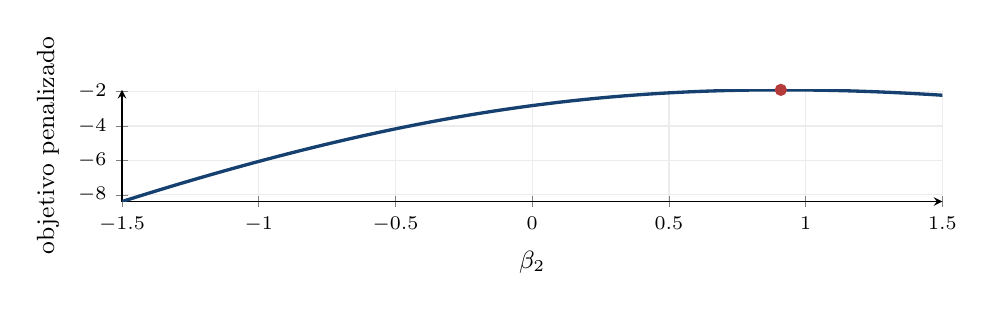
\begin{tikzpicture}
\begin{axis}[base,width=12cm,height=3cm,xmin=-1.5,xmax=1.5,xlabel={$\beta_2$},ylabel={objetivo penalizado}]
\addplot[azul,very thick] coordinates {(-1.50000,-8.39316870) (-1.45312,-8.15790483) (-1.40625,-7.92587441) (-1.35938,-7.69712888) (-1.31250,-7.47172224) (-1.26562,-7.24971118) (-1.21875,-7.03115514) (-1.17188,-6.81611639) (-1.12500,-6.60466010) (-1.07812,-6.39685438) (-1.03125,-6.19277028) (-0.98438,-5.99248180) (-0.93750,-5.79606582) (-0.89062,-5.60360206) (-0.84375,-5.41517286) (-0.79688,-5.23086311) (-0.75000,-5.05075989) (-0.70312,-4.87495222) (-0.65625,-4.70353065) (-0.60938,-4.53658683) (-0.56250,-4.37421291) (-0.51562,-4.21650098) (-0.46875,-4.06354232) (-0.42188,-3.91542668) (-0.37500,-3.77224142) (-0.32812,-3.63407061) (-0.28125,-3.50099410) (-0.23438,-3.37308660) (-0.18750,-3.25041672) (-0.14062,-3.13304604) (-0.09375,-3.02102822) (-0.04688,-2.91440823) (0.00000,-2.81322165) (0.04688,-2.71749408) (0.09375,-2.62724073) (0.14062,-2.54246613) (0.18750,-2.46316403) (0.23438,-2.38931748) (0.28125,-2.32089908) (0.32812,-2.25787136) (0.37500,-2.20018735) (0.42188,-2.14779125) (0.46875,-2.10061923) (0.51562,-2.05860027) (0.56250,-2.02165715) (0.60938,-1.98970733) (0.65625,-1.96266399) (0.70312,-1.94043692) (0.75000,-1.92293346) (0.79688,-1.91005936) (0.84375,-1.90171958) (0.89062,-1.89781902) (0.93750,-1.89826315) (0.98438,-1.90295861) (1.03125,-1.91181367) (1.07812,-1.92473863) (1.12500,-1.94164620) (1.17188,-1.96245172) (1.21875,-1.98707339) (1.26562,-2.01543240) (1.31250,-2.04745302) (1.35938,-2.08306267) (1.40625,-2.12219193) (1.45312,-2.16477450) (1.50000,-2.21074720)};\addplot[rojo,only marks,mark=*] coordinates {(0.90918141,-1.89748053)};
\end{axis}
\end{tikzpicture}
\caption{Objetivo penalizado al mover \(\beta_2\), fijando \(\beta_1\) en su solución para esta muestra.}
\end{figure}

La suma de los dieciséis aportes forma los momentos finitos.
Una muestra con baja probabilidad tiene menos peso,
aunque sus coeficientes puedan ser de magnitud grande.
La gráfica es un corte de la función de dos variables;
mantiene fijo el intercepto, y no es un perfil reoptimizado.
\endgroup

\clearpage
\section{Muestra 0100: raíz penalizada y aporte a los momentos}\label{logit129}
\begingroup\small
\setlength{\abovedisplayskip}{4pt}\setlength{\belowdisplayskip}{4pt}
Se mantienen las cuatro filas del experimento y se observa
la siguiente configuración de respuestas:
\[
y=\begin{pmatrix}0\\1\\0\\0\end{pmatrix},\quad \Prob(Y=y\mid X)=\frac{2}{3}\cdot\frac{1}{2}\cdot\frac{1}{3}\cdot\frac{1}{5}=\frac{1}{45}.
\]

El conteo de unos y el producto con el segundo regresor son
\[
\sum_{i=1}^4 y_i=1,\qquad\sum_{i=1}^4x_{i2}y_i=(-1)(0)+0(1)+1(0)+2(0)=0.
\]

En las ecuaciones abiertas de la unidad anterior se sustituyen
estos dos resultados. En el inicio, el sistema produce
\[
\begin{pmatrix}2&1/2\\1/2&5/2\end{pmatrix}\Delta^{(0)}=\begin{pmatrix}-1\\-1\end{pmatrix},\qquad\Delta^{(0)}=\begin{pmatrix}-0.42105263\\-0.31578947\end{pmatrix}.
\]

Se recalculan probabilidades y curvatura hasta resolver
ambas ecuaciones. La solución y el objetivo penalizado son
\[
\widehat\beta(y)\approx\begin{pmatrix}-0.43370094\\-0.33703771\end{pmatrix},\qquad \ell(\widehat\beta(y))-\tfrac12\|\widehat\beta(y)\|_2^2\approx-2.3958195269.
\]

La sustitución final en cada fila permite verificar
los dos gradientes, incluyendo el término de penalización.
\begin{center}\scriptsize
\begin{tabular}{rrrrrrr}\toprule
\(i\)&\(x_{i2}\)&\(y_i\)&\(\widehat\beta_1+x_{i2}\widehat\beta_2\)&probabilidad&discrepancia&varianza\\\midrule
1&-1&0&-0.09666323&0.47585299&-0.47585299&0.24941692\\
2&0&1&-0.43370094&0.39324293&0.60675707&0.23860293\\
3&1&0&-0.77073865&0.31631934&-0.31631934&0.21626142\\
4&2&0&-1.10777635&0.24828568&-0.24828568&0.18663990\\
\\\bottomrule\end{tabular}\end{center}
La suma de discrepancias coincide con \(\widehat\beta_1\).
La suma de \(x_{i2}\) por discrepancia coincide con
\(\widehat\beta_2\). Los residuos de ambas ecuaciones
tienen valor absoluto menor que \(10^{-10}\).

La curvatura positiva penalizada en la raíz es
\[
\begin{pmatrix}1.89092117&0.34012429\\0.34012429&2.21223794\end{pmatrix}.
\]

La muestra aporta a la esperanza su probabilidad
multiplicada por el vector de coeficientes:
\[
\frac{1}{45}\,\begin{pmatrix}-0.43370094\\-0.33703771\end{pmatrix}=\begin{pmatrix}-0.00963780\\-0.00748973\end{pmatrix}.
\]

A los segundos momentos aporta esa misma probabilidad
por todos los productos de coeficientes, incluidos los cruzados:
\[
\frac{1}{45}\,\begin{pmatrix}0.18809651&0.14617357\\0.14617357&0.11359442\end{pmatrix}.
\]

\begin{figure}[H]\centering
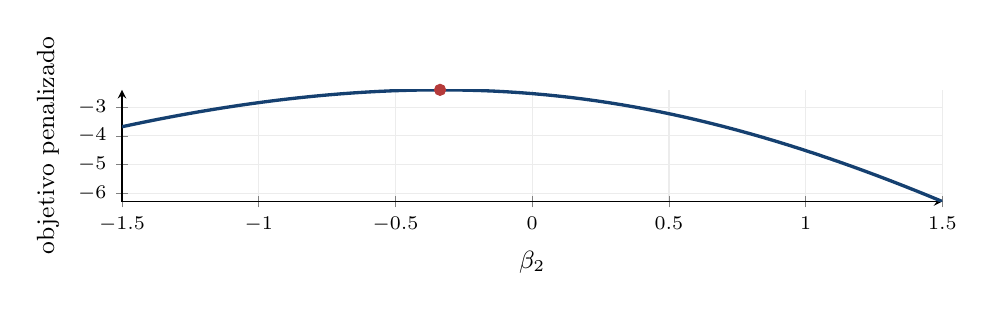
\begin{tikzpicture}
\begin{axis}[base,width=12cm,height=3cm,xmin=-1.5,xmax=1.5,xlabel={$\beta_2$},ylabel={objetivo penalizado}]
\addplot[azul,very thick] coordinates {(-1.50000,-3.68135719) (-1.45312,-3.58659676) (-1.40625,-3.49500352) (-1.35938,-3.40662200) (-1.31250,-3.32149888) (-1.26562,-3.23968311) (-1.21875,-3.16122601) (-1.17188,-3.08618134) (-1.12500,-3.01460541) (-1.07812,-2.94655718) (-1.03125,-2.88209827) (-0.98438,-2.82129308) (-0.93750,-2.76420879) (-0.89062,-2.71091537) (-0.84375,-2.66148556) (-0.79688,-2.61599483) (-0.75000,-2.57452125) (-0.70312,-2.53714536) (-0.65625,-2.50394994) (-0.60938,-2.47501980) (-0.56250,-2.45044136) (-0.51562,-2.43030231) (-0.46875,-2.41469107) (-0.42188,-2.40369627) (-0.37500,-2.39740608) (-0.32812,-2.39590749) (-0.28125,-2.39928553) (-0.23438,-2.40762243) (-0.18750,-2.42099669) (-0.14062,-2.43948222) (-0.09375,-2.46314734) (-0.04688,-2.49205388) (0.00000,-2.52625631) (0.04688,-2.56580091) (0.09375,-2.61072501) (0.14062,-2.66105640) (0.18750,-2.71681283) (0.23438,-2.77800164) (0.28125,-2.84461963) (0.32812,-2.91665302) (0.37500,-2.99407765) (0.42188,-3.07685925) (0.46875,-3.16495400) (0.51562,-3.25830907) (0.56250,-3.35686345) (0.60938,-3.46054868) (0.65625,-3.56928984) (0.70312,-3.68300644) (0.75000,-3.80161338) (0.79688,-3.92502193) (0.84375,-4.05314061) (0.89062,-4.18587611) (0.93750,-4.32313411) (0.98438,-4.46481997) (1.03125,-4.61083952) (1.07812,-4.76109952) (1.12500,-4.91550831) (1.17188,-5.07397612) (1.21875,-5.23641555) (1.26562,-5.40274175) (1.31250,-5.57287271) (1.35938,-5.74672940) (1.40625,-5.92423588) (1.45312,-6.10531936) (1.50000,-6.28991023)};\addplot[rojo,only marks,mark=*] coordinates {(-0.33703771,-2.39581953)};
\end{axis}
\end{tikzpicture}
\caption{Objetivo penalizado al mover \(\beta_2\), fijando \(\beta_1\) en su solución para esta muestra.}
\end{figure}

La suma de los dieciséis aportes forma los momentos finitos.
Una muestra con baja probabilidad tiene menos peso,
aunque sus coeficientes puedan ser de magnitud grande.
La gráfica es un corte de la función de dos variables;
mantiene fijo el intercepto, y no es un perfil reoptimizado.
\endgroup

\clearpage
\section{Muestra 0101: raíz penalizada y aporte a los momentos}\label{logit130}
\begingroup\small
\setlength{\abovedisplayskip}{4pt}\setlength{\belowdisplayskip}{4pt}
Se mantienen las cuatro filas del experimento y se observa
la siguiente configuración de respuestas:
\[
y=\begin{pmatrix}0\\1\\0\\1\end{pmatrix},\quad \Prob(Y=y\mid X)=\frac{2}{3}\cdot\frac{1}{2}\cdot\frac{1}{3}\cdot\frac{4}{5}=\frac{4}{45}.
\]

El conteo de unos y el producto con el segundo regresor son
\[
\sum_{i=1}^4 y_i=2,\qquad\sum_{i=1}^4x_{i2}y_i=(-1)(0)+0(1)+1(0)+2(1)=2.
\]

En las ecuaciones abiertas de la unidad anterior se sustituyen
estos dos resultados. En el inicio, el sistema produce
\[
\begin{pmatrix}2&1/2\\1/2&5/2\end{pmatrix}\Delta^{(0)}=\begin{pmatrix}0\\1\end{pmatrix},\qquad\Delta^{(0)}=\begin{pmatrix}-0.10526316\\0.42105263\end{pmatrix}.
\]

Se recalculan probabilidades y curvatura hasta resolver
ambas ecuaciones. La solución y el objetivo penalizado son
\[
\widehat\beta(y)\approx\begin{pmatrix}-0.10425081\\0.42912255\end{pmatrix},\qquad \ell(\widehat\beta(y))-\tfrac12\|\widehat\beta(y)\|_2^2\approx-2.5600548260.
\]

La sustitución final en cada fila permite verificar
los dos gradientes, incluyendo el término de penalización.
\begin{center}\scriptsize
\begin{tabular}{rrrrrrr}\toprule
\(i\)&\(x_{i2}\)&\(y_i\)&\(\widehat\beta_1+x_{i2}\widehat\beta_2\)&probabilidad&discrepancia&varianza\\\midrule
1&-1&0&-0.53337336&0.36973045&-0.36973045&0.23302984\\
2&0&1&-0.10425081&0.47396088&0.52603912&0.24932196\\
3&1&0&0.32487174&0.58051107&-0.58051107&0.24351797\\
4&2&1&0.75399429&0.68004841&0.31995159&0.21758257\\
\\\bottomrule\end{tabular}\end{center}
La suma de discrepancias coincide con \(\widehat\beta_1\).
La suma de \(x_{i2}\) por discrepancia coincide con
\(\widehat\beta_2\). Los residuos de ambas ecuaciones
tienen valor absoluto menor que \(10^{-10}\).

La curvatura positiva penalizada en la raíz es
\[
\begin{pmatrix}1.94345234&0.44565326\\0.44565326&2.34687809\end{pmatrix}.
\]

La muestra aporta a la esperanza su probabilidad
multiplicada por el vector de coeficientes:
\[
\frac{4}{45}\,\begin{pmatrix}-0.10425081\\0.42912255\end{pmatrix}=\begin{pmatrix}-0.00926674\\0.03814423\end{pmatrix}.
\]

A los segundos momentos aporta esa misma probabilidad
por todos los productos de coeficientes, incluidos los cruzados:
\[
\frac{4}{45}\,\begin{pmatrix}0.01086823&-0.04473637\\-0.04473637&0.18414616\end{pmatrix}.
\]

\begin{figure}[H]\centering
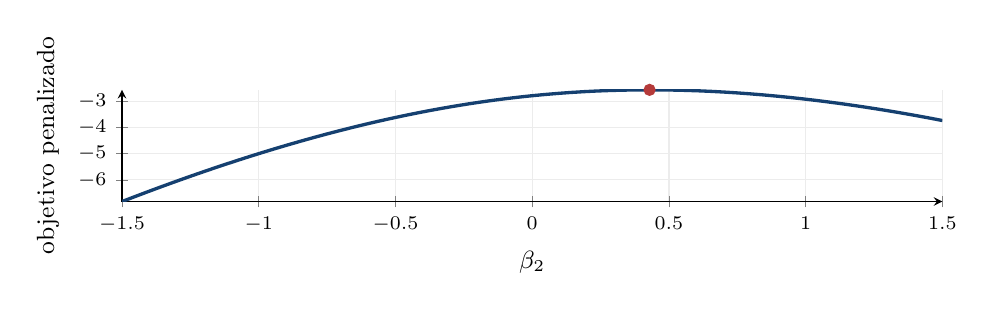
\begin{tikzpicture}
\begin{axis}[base,width=12cm,height=3cm,xmin=-1.5,xmax=1.5,xlabel={$\beta_2$},ylabel={objetivo penalizado}]
\addplot[azul,very thick] coordinates {(-1.50000,-6.82539338) (-1.45312,-6.63724700) (-1.40625,-6.45236671) (-1.35938,-6.27080681) (-1.31250,-6.09262436) (-1.26562,-5.91787921) (-1.21875,-5.74663413) (-1.17188,-5.57895484) (-1.12500,-5.41491007) (-1.07812,-5.25457154) (-1.03125,-5.09801401) (-0.98438,-4.94531516) (-0.93750,-4.79655556) (-0.89062,-4.65181851) (-0.84375,-4.51118983) (-0.79688,-4.37475765) (-0.75000,-4.24261205) (-0.70312,-4.11484467) (-0.65625,-3.99154830) (-0.60938,-3.87281624) (-0.56250,-3.75874174) (-0.51562,-3.64941728) (-0.46875,-3.54493378) (-0.42188,-3.44537975) (-0.37500,-3.35084044) (-0.32812,-3.26139683) (-0.28125,-3.17712475) (-0.23438,-3.09809386) (-0.18750,-3.02436677) (-0.14062,-2.95599815) (-0.09375,-2.89303392) (-0.04688,-2.83551055) (0.00000,-2.78345449) (0.04688,-2.73688177) (0.09375,-2.69579768) (0.14062,-2.66019668) (0.18750,-2.63006251) (0.23438,-2.60536841) (0.28125,-2.58607751) (0.32812,-2.57214342) (0.37500,-2.56351086) (0.42188,-2.56011651) (0.46875,-2.56188985) (0.51562,-2.56875410) (0.56250,-2.58062715) (0.60938,-2.59742256) (0.65625,-2.61905050) (0.70312,-2.64541863) (0.75000,-2.67643302) (0.79688,-2.71199888) (0.84375,-2.75202136) (0.89062,-2.79640612) (0.93750,-2.84505997) (0.98438,-2.89789129) (1.03125,-2.95481049) (1.07812,-3.01573032) (1.12500,-3.08056614) (1.17188,-3.14923613) (1.21875,-3.22166141) (1.26562,-3.29776617) (1.31250,-3.37747772) (1.35938,-3.46072646) (1.40625,-3.54744592) (1.45312,-3.63757270) (1.50000,-3.73104639)};\addplot[rojo,only marks,mark=*] coordinates {(0.42912255,-2.56005483)};
\end{axis}
\end{tikzpicture}
\caption{Objetivo penalizado al mover \(\beta_2\), fijando \(\beta_1\) en su solución para esta muestra.}
\end{figure}

La suma de los dieciséis aportes forma los momentos finitos.
Una muestra con baja probabilidad tiene menos peso,
aunque sus coeficientes puedan ser de magnitud grande.
La gráfica es un corte de la función de dos variables;
mantiene fijo el intercepto, y no es un perfil reoptimizado.
\endgroup

\clearpage
\section{Muestra 0110: raíz penalizada y aporte a los momentos}\label{logit131}
\begingroup\small
\setlength{\abovedisplayskip}{4pt}\setlength{\belowdisplayskip}{4pt}
Se mantienen las cuatro filas del experimento y se observa
la siguiente configuración de respuestas:
\[
y=\begin{pmatrix}0\\1\\1\\0\end{pmatrix},\quad \Prob(Y=y\mid X)=\frac{2}{3}\cdot\frac{1}{2}\cdot\frac{2}{3}\cdot\frac{1}{5}=\frac{2}{45}.
\]

El conteo de unos y el producto con el segundo regresor son
\[
\sum_{i=1}^4 y_i=2,\qquad\sum_{i=1}^4x_{i2}y_i=(-1)(0)+0(1)+1(1)+2(0)=1.
\]

En las ecuaciones abiertas de la unidad anterior se sustituyen
estos dos resultados. En el inicio, el sistema produce
\[
\begin{pmatrix}2&1/2\\1/2&5/2\end{pmatrix}\Delta^{(0)}=\begin{pmatrix}0\\0\end{pmatrix},\qquad\Delta^{(0)}=\begin{pmatrix}0\\0\end{pmatrix}.
\]

Se recalculan probabilidades y curvatura hasta resolver
ambas ecuaciones. La solución y el objetivo penalizado son
\[
\widehat\beta(y)\approx\begin{pmatrix}0\\0\end{pmatrix},\qquad \ell(\widehat\beta(y))-\tfrac12\|\widehat\beta(y)\|_2^2\approx-2.7725887222.
\]

La sustitución final en cada fila permite verificar
los dos gradientes, incluyendo el término de penalización.
\begin{center}\scriptsize
\begin{tabular}{rrrrrrr}\toprule
\(i\)&\(x_{i2}\)&\(y_i\)&\(\widehat\beta_1+x_{i2}\widehat\beta_2\)&probabilidad&discrepancia&varianza\\\midrule
1&-1&0&0.00000000&0.50000000&-0.50000000&0.25000000\\
2&0&1&0.00000000&0.50000000&0.50000000&0.25000000\\
3&1&1&0.00000000&0.50000000&0.50000000&0.25000000\\
4&2&0&0.00000000&0.50000000&-0.50000000&0.25000000\\
\\\bottomrule\end{tabular}\end{center}
La suma de discrepancias coincide con \(\widehat\beta_1\).
La suma de \(x_{i2}\) por discrepancia coincide con
\(\widehat\beta_2\). Los residuos de ambas ecuaciones
tienen valor absoluto menor que \(10^{-10}\).

La curvatura positiva penalizada en la raíz es
\[
\begin{pmatrix}2.00000000&0.50000000\\0.50000000&2.50000000\end{pmatrix}.
\]

La muestra aporta a la esperanza su probabilidad
multiplicada por el vector de coeficientes:
\[
\frac{2}{45}\,\begin{pmatrix}0\\0\end{pmatrix}=\begin{pmatrix}0\\0\end{pmatrix}.
\]

A los segundos momentos aporta esa misma probabilidad
por todos los productos de coeficientes, incluidos los cruzados:
\[
\frac{2}{45}\,\begin{pmatrix}0&0\\0&0\end{pmatrix}.
\]

\begin{figure}[H]\centering
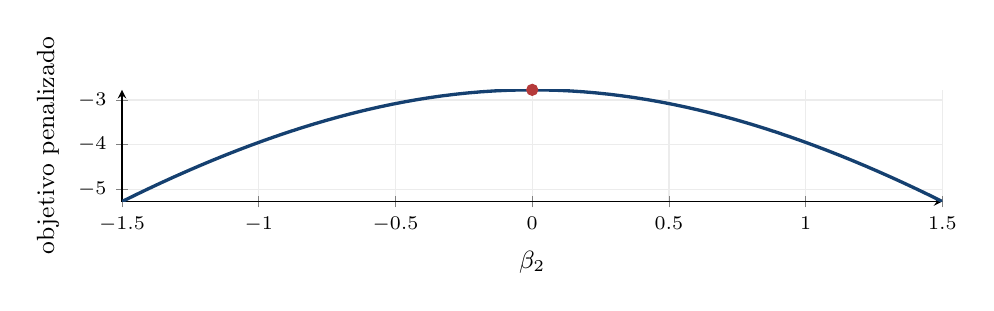
\begin{tikzpicture}
\begin{axis}[base,width=12cm,height=3cm,xmin=-1.5,xmax=1.5,xlabel={$\beta_2$},ylabel={objetivo penalizado}]
\addplot[azul,very thick] coordinates {(-1.50000,-5.26956109) (-1.45312,-5.12868102) (-1.40625,-4.99110550) (-1.35938,-4.85689192) (-1.31250,-4.72610052) (-1.26562,-4.59879452) (-1.21875,-4.47504014) (-1.17188,-4.35490669) (-1.12500,-4.23846651) (-1.07812,-4.12579505) (-1.03125,-4.01697074) (-0.98438,-3.91207494) (-0.93750,-3.81119178) (-0.89062,-3.71440797) (-0.84375,-3.62181254) (-0.79688,-3.53349650) (-0.75000,-3.44955247) (-0.70312,-3.37007415) (-0.65625,-3.29515582) (-0.60938,-3.22489164) (-0.56250,-3.15937500) (-0.51562,-3.09869768) (-0.46875,-3.04294900) (-0.42188,-2.99221495) (-0.37500,-2.94657721) (-0.32812,-2.90611221) (-0.28125,-2.87089016) (-0.23438,-2.84097412) (-0.18750,-2.81641915) (-0.14062,-2.79727147) (-0.09375,-2.78356782) (-0.04688,-2.77533485) (0.00000,-2.77258872) (0.04688,-2.77533485) (0.09375,-2.78356782) (0.14062,-2.79727147) (0.18750,-2.81641915) (0.23438,-2.84097412) (0.28125,-2.87089016) (0.32812,-2.90611221) (0.37500,-2.94657721) (0.42188,-2.99221495) (0.46875,-3.04294900) (0.51562,-3.09869768) (0.56250,-3.15937500) (0.60938,-3.22489164) (0.65625,-3.29515582) (0.70312,-3.37007415) (0.75000,-3.44955247) (0.79688,-3.53349650) (0.84375,-3.62181254) (0.89062,-3.71440797) (0.93750,-3.81119178) (0.98438,-3.91207494) (1.03125,-4.01697074) (1.07812,-4.12579505) (1.12500,-4.23846651) (1.17188,-4.35490669) (1.21875,-4.47504014) (1.26562,-4.59879452) (1.31250,-4.72610052) (1.35938,-4.85689192) (1.40625,-4.99110550) (1.45312,-5.12868102) (1.50000,-5.26956109)};\addplot[rojo,only marks,mark=*] coordinates {(0.00000000,-2.77258872)};
\end{axis}
\end{tikzpicture}
\caption{Objetivo penalizado al mover \(\beta_2\), fijando \(\beta_1\) en su solución para esta muestra.}
\end{figure}

La suma de los dieciséis aportes forma los momentos finitos.
Una muestra con baja probabilidad tiene menos peso,
aunque sus coeficientes puedan ser de magnitud grande.
La gráfica es un corte de la función de dos variables;
mantiene fijo el intercepto, y no es un perfil reoptimizado.
\endgroup

\clearpage
\section{Muestra 0111: raíz penalizada y aporte a los momentos}\label{logit132}
\begingroup\small
\setlength{\abovedisplayskip}{4pt}\setlength{\belowdisplayskip}{4pt}
Se mantienen las cuatro filas del experimento y se observa
la siguiente configuración de respuestas:
\[
y=\begin{pmatrix}0\\1\\1\\1\end{pmatrix},\quad \Prob(Y=y\mid X)=\frac{2}{3}\cdot\frac{1}{2}\cdot\frac{2}{3}\cdot\frac{4}{5}=\frac{8}{45}.
\]

El conteo de unos y el producto con el segundo regresor son
\[
\sum_{i=1}^4 y_i=3,\qquad\sum_{i=1}^4x_{i2}y_i=(-1)(0)+0(1)+1(1)+2(1)=3.
\]

En las ecuaciones abiertas de la unidad anterior se sustituyen
estos dos resultados. En el inicio, el sistema produce
\[
\begin{pmatrix}2&1/2\\1/2&5/2\end{pmatrix}\Delta^{(0)}=\begin{pmatrix}1\\2\end{pmatrix},\qquad\Delta^{(0)}=\begin{pmatrix}0.31578947\\0.73684211\end{pmatrix}.
\]

Se recalculan probabilidades y curvatura hasta resolver
ambas ecuaciones. La solución y el objetivo penalizado son
\[
\widehat\beta(y)\approx\begin{pmatrix}0.36856083\\0.84144532\end{pmatrix},\qquad \ell(\widehat\beta(y))-\tfrac12\|\widehat\beta(y)\|_2^2\approx-1.8139927856.
\]

La sustitución final en cada fila permite verificar
los dos gradientes, incluyendo el término de penalización.
\begin{center}\scriptsize
\begin{tabular}{rrrrrrr}\toprule
\(i\)&\(x_{i2}\)&\(y_i\)&\(\widehat\beta_1+x_{i2}\widehat\beta_2\)&probabilidad&discrepancia&varianza\\\midrule
1&-1&0&-0.47288448&0.38393375&-0.38393375&0.23652863\\
2&0&1&0.36856083&0.59111118&0.40888882&0.24169875\\
3&1&1&1.21000615&0.77030004&0.22969996&0.17693789\\
4&2&1&2.05145147&0.88609420&0.11390580&0.10093127\\
\\\bottomrule\end{tabular}\end{center}
La suma de discrepancias coincide con \(\widehat\beta_1\).
La suma de \(x_{i2}\) por discrepancia coincide con
\(\widehat\beta_2\). Los residuos de ambas ecuaciones
tienen valor absoluto menor que \(10^{-10}\).

La curvatura positiva penalizada en la raíz es
\[
\begin{pmatrix}1.75609654&0.14227180\\0.14227180&1.81719159\end{pmatrix}.
\]

La muestra aporta a la esperanza su probabilidad
multiplicada por el vector de coeficientes:
\[
\frac{8}{45}\,\begin{pmatrix}0.36856083\\0.84144532\end{pmatrix}=\begin{pmatrix}0.06552193\\0.14959028\end{pmatrix}.
\]

A los segundos momentos aporta esa misma probabilidad
por todos los productos de coeficientes, incluidos los cruzados:
\[
\frac{8}{45}\,\begin{pmatrix}0.13583709&0.31012379\\0.31012379&0.70803022\end{pmatrix}.
\]

\begin{figure}[H]\centering
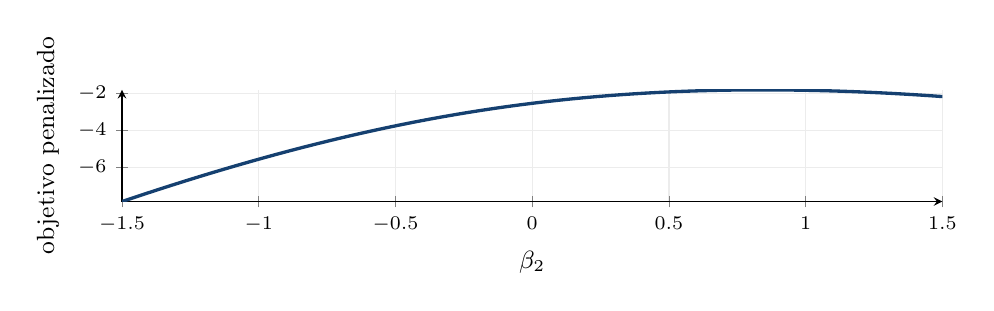
\begin{tikzpicture}
\begin{axis}[base,width=12cm,height=3cm,xmin=-1.5,xmax=1.5,xlabel={$\beta_2$},ylabel={objetivo penalizado}]
\addplot[azul,very thick] coordinates {(-1.50000,-7.84272088) (-1.45312,-7.61061754) (-1.40625,-7.38198664) (-1.35938,-7.15689603) (-1.31250,-6.93541675) (-1.26562,-6.71762298) (-1.21875,-6.50359208) (-1.17188,-6.29340444) (-1.12500,-6.08714338) (-1.07812,-5.88489497) (-1.03125,-5.68674781) (-0.98438,-5.49279265) (-0.93750,-5.30312207) (-0.89062,-5.11783000) (-0.84375,-4.93701115) (-0.79688,-4.76076042) (-0.75000,-4.58917219) (-0.70312,-4.42233952) (-0.65625,-4.26035334) (-0.60938,-4.10330150) (-0.56250,-3.95126791) (-0.51562,-3.80433151) (-0.46875,-3.66256535) (-0.42188,-3.52603564) (-0.37500,-3.39480088) (-0.32812,-3.26891104) (-0.28125,-3.14840686) (-0.23438,-3.03331928) (-0.18750,-2.92366896) (-0.14062,-2.81946605) (-0.09375,-2.72071005) (-0.04688,-2.62738985) (0.00000,-2.53948401) (0.04688,-2.45696111) (0.09375,-2.37978029) (0.14062,-2.30789192) (0.18750,-2.24123836) (0.23438,-2.17975484) (0.28125,-2.12337032) (0.32812,-2.07200843) (0.37500,-2.02558845) (0.42188,-1.98402618) (0.46875,-1.94723485) (0.51562,-1.91512598) (0.56250,-1.88761009) (0.60938,-1.86459748) (0.65625,-1.84599879) (0.70312,-1.83172559) (0.75000,-1.82169083) (0.79688,-1.81580923) (0.84375,-1.81399761) (0.89062,-1.81617514) (0.93750,-1.82226352) (0.98438,-1.83218717) (1.03125,-1.84587323) (1.07812,-1.86325169) (1.12500,-1.88425540) (1.17188,-1.90881998) (1.21875,-1.93688387) (1.26562,-1.96838823) (1.31250,-2.00327688) (1.35938,-2.04149619) (1.40625,-2.08299503) (1.45312,-2.12772465) (1.50000,-2.17563857)};\addplot[rojo,only marks,mark=*] coordinates {(0.84144532,-1.81399279)};
\end{axis}
\end{tikzpicture}
\caption{Objetivo penalizado al mover \(\beta_2\), fijando \(\beta_1\) en su solución para esta muestra.}
\end{figure}

La suma de los dieciséis aportes forma los momentos finitos.
Una muestra con baja probabilidad tiene menos peso,
aunque sus coeficientes puedan ser de magnitud grande.
La gráfica es un corte de la función de dos variables;
mantiene fijo el intercepto, y no es un perfil reoptimizado.
\endgroup

\clearpage
\section{Muestra 1000: raíz penalizada y aporte a los momentos}\label{logit133}
\begingroup\small
\setlength{\abovedisplayskip}{4pt}\setlength{\belowdisplayskip}{4pt}
Se mantienen las cuatro filas del experimento y se observa
la siguiente configuración de respuestas:
\[
y=\begin{pmatrix}1\\0\\0\\0\end{pmatrix},\quad \Prob(Y=y\mid X)=\frac{1}{3}\cdot\frac{1}{2}\cdot\frac{1}{3}\cdot\frac{1}{5}=\frac{1}{90}.
\]

El conteo de unos y el producto con el segundo regresor son
\[
\sum_{i=1}^4 y_i=1,\qquad\sum_{i=1}^4x_{i2}y_i=(-1)(1)+0(0)+1(0)+2(0)=-1.
\]

En las ecuaciones abiertas de la unidad anterior se sustituyen
estos dos resultados. En el inicio, el sistema produce
\[
\begin{pmatrix}2&1/2\\1/2&5/2\end{pmatrix}\Delta^{(0)}=\begin{pmatrix}-1\\-2\end{pmatrix},\qquad\Delta^{(0)}=\begin{pmatrix}-0.31578947\\-0.73684211\end{pmatrix}.
\]

Se recalculan probabilidades y curvatura hasta resolver
ambas ecuaciones. La solución y el objetivo penalizado son
\[
\widehat\beta(y)\approx\begin{pmatrix}-0.36856083\\-0.84144532\end{pmatrix},\qquad \ell(\widehat\beta(y))-\tfrac12\|\widehat\beta(y)\|_2^2\approx-1.8139927856.
\]

La sustitución final en cada fila permite verificar
los dos gradientes, incluyendo el término de penalización.
\begin{center}\scriptsize
\begin{tabular}{rrrrrrr}\toprule
\(i\)&\(x_{i2}\)&\(y_i\)&\(\widehat\beta_1+x_{i2}\widehat\beta_2\)&probabilidad&discrepancia&varianza\\\midrule
1&-1&1&0.47288448&0.61606625&0.38393375&0.23652863\\
2&0&0&-0.36856083&0.40888882&-0.40888882&0.24169875\\
3&1&0&-1.21000615&0.22969996&-0.22969996&0.17693789\\
4&2&0&-2.05145147&0.11390580&-0.11390580&0.10093127\\
\\\bottomrule\end{tabular}\end{center}
La suma de discrepancias coincide con \(\widehat\beta_1\).
La suma de \(x_{i2}\) por discrepancia coincide con
\(\widehat\beta_2\). Los residuos de ambas ecuaciones
tienen valor absoluto menor que \(10^{-10}\).

La curvatura positiva penalizada en la raíz es
\[
\begin{pmatrix}1.75609654&0.14227180\\0.14227180&1.81719159\end{pmatrix}.
\]

La muestra aporta a la esperanza su probabilidad
multiplicada por el vector de coeficientes:
\[
\frac{1}{90}\,\begin{pmatrix}-0.36856083\\-0.84144532\end{pmatrix}=\begin{pmatrix}-0.00409512\\-0.00934939\end{pmatrix}.
\]

A los segundos momentos aporta esa misma probabilidad
por todos los productos de coeficientes, incluidos los cruzados:
\[
\frac{1}{90}\,\begin{pmatrix}0.13583709&0.31012379\\0.31012379&0.70803022\end{pmatrix}.
\]

\begin{figure}[H]\centering
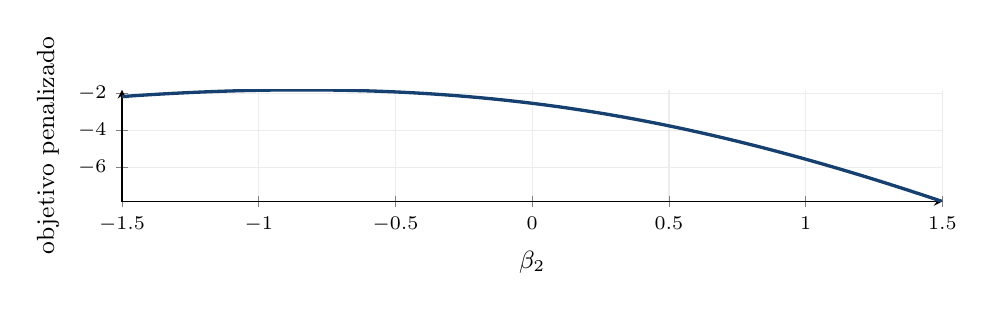
\begin{tikzpicture}
\begin{axis}[base,width=12cm,height=3cm,xmin=-1.5,xmax=1.5,xlabel={$\beta_2$},ylabel={objetivo penalizado}]
\addplot[azul,very thick] coordinates {(-1.50000,-2.17563857) (-1.45312,-2.12772465) (-1.40625,-2.08299503) (-1.35938,-2.04149619) (-1.31250,-2.00327688) (-1.26562,-1.96838823) (-1.21875,-1.93688387) (-1.17188,-1.90881998) (-1.12500,-1.88425540) (-1.07812,-1.86325169) (-1.03125,-1.84587323) (-0.98438,-1.83218717) (-0.93750,-1.82226352) (-0.89062,-1.81617514) (-0.84375,-1.81399761) (-0.79688,-1.81580923) (-0.75000,-1.82169083) (-0.70312,-1.83172559) (-0.65625,-1.84599879) (-0.60938,-1.86459748) (-0.56250,-1.88761009) (-0.51562,-1.91512598) (-0.46875,-1.94723485) (-0.42188,-1.98402618) (-0.37500,-2.02558845) (-0.32812,-2.07200843) (-0.28125,-2.12337032) (-0.23438,-2.17975484) (-0.18750,-2.24123836) (-0.14062,-2.30789192) (-0.09375,-2.37978029) (-0.04688,-2.45696111) (0.00000,-2.53948401) (0.04688,-2.62738985) (0.09375,-2.72071005) (0.14062,-2.81946605) (0.18750,-2.92366896) (0.23438,-3.03331928) (0.28125,-3.14840686) (0.32812,-3.26891104) (0.37500,-3.39480088) (0.42188,-3.52603564) (0.46875,-3.66256535) (0.51562,-3.80433151) (0.56250,-3.95126791) (0.60938,-4.10330150) (0.65625,-4.26035334) (0.70312,-4.42233952) (0.75000,-4.58917219) (0.79688,-4.76076042) (0.84375,-4.93701115) (0.89062,-5.11783000) (0.93750,-5.30312207) (0.98438,-5.49279265) (1.03125,-5.68674781) (1.07812,-5.88489497) (1.12500,-6.08714338) (1.17188,-6.29340444) (1.21875,-6.50359208) (1.26562,-6.71762298) (1.31250,-6.93541675) (1.35938,-7.15689603) (1.40625,-7.38198664) (1.45312,-7.61061754) (1.50000,-7.84272088)};\addplot[rojo,only marks,mark=*] coordinates {(-0.84144532,-1.81399279)};
\end{axis}
\end{tikzpicture}
\caption{Objetivo penalizado al mover \(\beta_2\), fijando \(\beta_1\) en su solución para esta muestra.}
\end{figure}

La suma de los dieciséis aportes forma los momentos finitos.
Una muestra con baja probabilidad tiene menos peso,
aunque sus coeficientes puedan ser de magnitud grande.
La gráfica es un corte de la función de dos variables;
mantiene fijo el intercepto, y no es un perfil reoptimizado.
\endgroup

\clearpage
\section{Muestra 1001: raíz penalizada y aporte a los momentos}\label{logit134}
\begingroup\small
\setlength{\abovedisplayskip}{4pt}\setlength{\belowdisplayskip}{4pt}
Se mantienen las cuatro filas del experimento y se observa
la siguiente configuración de respuestas:
\[
y=\begin{pmatrix}1\\0\\0\\1\end{pmatrix},\quad \Prob(Y=y\mid X)=\frac{1}{3}\cdot\frac{1}{2}\cdot\frac{1}{3}\cdot\frac{4}{5}=\frac{2}{45}.
\]

El conteo de unos y el producto con el segundo regresor son
\[
\sum_{i=1}^4 y_i=2,\qquad\sum_{i=1}^4x_{i2}y_i=(-1)(1)+0(0)+1(0)+2(1)=1.
\]

En las ecuaciones abiertas de la unidad anterior se sustituyen
estos dos resultados. En el inicio, el sistema produce
\[
\begin{pmatrix}2&1/2\\1/2&5/2\end{pmatrix}\Delta^{(0)}=\begin{pmatrix}0\\0\end{pmatrix},\qquad\Delta^{(0)}=\begin{pmatrix}0\\0\end{pmatrix}.
\]

Se recalculan probabilidades y curvatura hasta resolver
ambas ecuaciones. La solución y el objetivo penalizado son
\[
\widehat\beta(y)\approx\begin{pmatrix}0\\0\end{pmatrix},\qquad \ell(\widehat\beta(y))-\tfrac12\|\widehat\beta(y)\|_2^2\approx-2.7725887222.
\]

La sustitución final en cada fila permite verificar
los dos gradientes, incluyendo el término de penalización.
\begin{center}\scriptsize
\begin{tabular}{rrrrrrr}\toprule
\(i\)&\(x_{i2}\)&\(y_i\)&\(\widehat\beta_1+x_{i2}\widehat\beta_2\)&probabilidad&discrepancia&varianza\\\midrule
1&-1&1&0.00000000&0.50000000&0.50000000&0.25000000\\
2&0&0&0.00000000&0.50000000&-0.50000000&0.25000000\\
3&1&0&0.00000000&0.50000000&-0.50000000&0.25000000\\
4&2&1&0.00000000&0.50000000&0.50000000&0.25000000\\
\\\bottomrule\end{tabular}\end{center}
La suma de discrepancias coincide con \(\widehat\beta_1\).
La suma de \(x_{i2}\) por discrepancia coincide con
\(\widehat\beta_2\). Los residuos de ambas ecuaciones
tienen valor absoluto menor que \(10^{-10}\).

La curvatura positiva penalizada en la raíz es
\[
\begin{pmatrix}2.00000000&0.50000000\\0.50000000&2.50000000\end{pmatrix}.
\]

La muestra aporta a la esperanza su probabilidad
multiplicada por el vector de coeficientes:
\[
\frac{2}{45}\,\begin{pmatrix}0\\0\end{pmatrix}=\begin{pmatrix}0\\0\end{pmatrix}.
\]

A los segundos momentos aporta esa misma probabilidad
por todos los productos de coeficientes, incluidos los cruzados:
\[
\frac{2}{45}\,\begin{pmatrix}0&0\\0&0\end{pmatrix}.
\]

\begin{figure}[H]\centering
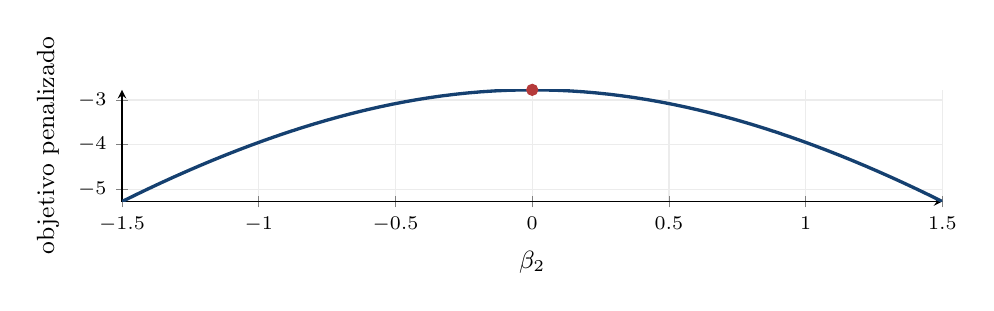
\begin{tikzpicture}
\begin{axis}[base,width=12cm,height=3cm,xmin=-1.5,xmax=1.5,xlabel={$\beta_2$},ylabel={objetivo penalizado}]
\addplot[azul,very thick] coordinates {(-1.50000,-5.26956109) (-1.45312,-5.12868102) (-1.40625,-4.99110550) (-1.35938,-4.85689192) (-1.31250,-4.72610052) (-1.26562,-4.59879452) (-1.21875,-4.47504014) (-1.17188,-4.35490669) (-1.12500,-4.23846651) (-1.07812,-4.12579505) (-1.03125,-4.01697074) (-0.98438,-3.91207494) (-0.93750,-3.81119178) (-0.89062,-3.71440797) (-0.84375,-3.62181254) (-0.79688,-3.53349650) (-0.75000,-3.44955247) (-0.70312,-3.37007415) (-0.65625,-3.29515582) (-0.60938,-3.22489164) (-0.56250,-3.15937500) (-0.51562,-3.09869768) (-0.46875,-3.04294900) (-0.42188,-2.99221495) (-0.37500,-2.94657721) (-0.32812,-2.90611221) (-0.28125,-2.87089016) (-0.23438,-2.84097412) (-0.18750,-2.81641915) (-0.14062,-2.79727147) (-0.09375,-2.78356782) (-0.04688,-2.77533485) (0.00000,-2.77258872) (0.04688,-2.77533485) (0.09375,-2.78356782) (0.14062,-2.79727147) (0.18750,-2.81641915) (0.23438,-2.84097412) (0.28125,-2.87089016) (0.32812,-2.90611221) (0.37500,-2.94657721) (0.42188,-2.99221495) (0.46875,-3.04294900) (0.51562,-3.09869768) (0.56250,-3.15937500) (0.60938,-3.22489164) (0.65625,-3.29515582) (0.70312,-3.37007415) (0.75000,-3.44955247) (0.79688,-3.53349650) (0.84375,-3.62181254) (0.89062,-3.71440797) (0.93750,-3.81119178) (0.98438,-3.91207494) (1.03125,-4.01697074) (1.07812,-4.12579505) (1.12500,-4.23846651) (1.17188,-4.35490669) (1.21875,-4.47504014) (1.26562,-4.59879452) (1.31250,-4.72610052) (1.35938,-4.85689192) (1.40625,-4.99110550) (1.45312,-5.12868102) (1.50000,-5.26956109)};\addplot[rojo,only marks,mark=*] coordinates {(0.00000000,-2.77258872)};
\end{axis}
\end{tikzpicture}
\caption{Objetivo penalizado al mover \(\beta_2\), fijando \(\beta_1\) en su solución para esta muestra.}
\end{figure}

La suma de los dieciséis aportes forma los momentos finitos.
Una muestra con baja probabilidad tiene menos peso,
aunque sus coeficientes puedan ser de magnitud grande.
La gráfica es un corte de la función de dos variables;
mantiene fijo el intercepto, y no es un perfil reoptimizado.
\endgroup

\clearpage
\section{Muestra 1010: raíz penalizada y aporte a los momentos}\label{logit135}
\begingroup\small
\setlength{\abovedisplayskip}{4pt}\setlength{\belowdisplayskip}{4pt}
Se mantienen las cuatro filas del experimento y se observa
la siguiente configuración de respuestas:
\[
y=\begin{pmatrix}1\\0\\1\\0\end{pmatrix},\quad \Prob(Y=y\mid X)=\frac{1}{3}\cdot\frac{1}{2}\cdot\frac{2}{3}\cdot\frac{1}{5}=\frac{1}{45}.
\]

El conteo de unos y el producto con el segundo regresor son
\[
\sum_{i=1}^4 y_i=2,\qquad\sum_{i=1}^4x_{i2}y_i=(-1)(1)+0(0)+1(1)+2(0)=0.
\]

En las ecuaciones abiertas de la unidad anterior se sustituyen
estos dos resultados. En el inicio, el sistema produce
\[
\begin{pmatrix}2&1/2\\1/2&5/2\end{pmatrix}\Delta^{(0)}=\begin{pmatrix}0\\-1\end{pmatrix},\qquad\Delta^{(0)}=\begin{pmatrix}0.10526316\\-0.42105263\end{pmatrix}.
\]

Se recalculan probabilidades y curvatura hasta resolver
ambas ecuaciones. La solución y el objetivo penalizado son
\[
\widehat\beta(y)\approx\begin{pmatrix}0.10425081\\-0.42912255\end{pmatrix},\qquad \ell(\widehat\beta(y))-\tfrac12\|\widehat\beta(y)\|_2^2\approx-2.5600548260.
\]

La sustitución final en cada fila permite verificar
los dos gradientes, incluyendo el término de penalización.
\begin{center}\scriptsize
\begin{tabular}{rrrrrrr}\toprule
\(i\)&\(x_{i2}\)&\(y_i\)&\(\widehat\beta_1+x_{i2}\widehat\beta_2\)&probabilidad&discrepancia&varianza\\\midrule
1&-1&1&0.53337336&0.63026955&0.36973045&0.23302984\\
2&0&0&0.10425081&0.52603912&-0.52603912&0.24932196\\
3&1&1&-0.32487174&0.41948893&0.58051107&0.24351797\\
4&2&0&-0.75399429&0.31995159&-0.31995159&0.21758257\\
\\\bottomrule\end{tabular}\end{center}
La suma de discrepancias coincide con \(\widehat\beta_1\).
La suma de \(x_{i2}\) por discrepancia coincide con
\(\widehat\beta_2\). Los residuos de ambas ecuaciones
tienen valor absoluto menor que \(10^{-10}\).

La curvatura positiva penalizada en la raíz es
\[
\begin{pmatrix}1.94345234&0.44565326\\0.44565326&2.34687809\end{pmatrix}.
\]

La muestra aporta a la esperanza su probabilidad
multiplicada por el vector de coeficientes:
\[
\frac{1}{45}\,\begin{pmatrix}0.10425081\\-0.42912255\end{pmatrix}=\begin{pmatrix}0.00231668\\-0.00953606\end{pmatrix}.
\]

A los segundos momentos aporta esa misma probabilidad
por todos los productos de coeficientes, incluidos los cruzados:
\[
\frac{1}{45}\,\begin{pmatrix}0.01086823&-0.04473637\\-0.04473637&0.18414616\end{pmatrix}.
\]

\begin{figure}[H]\centering
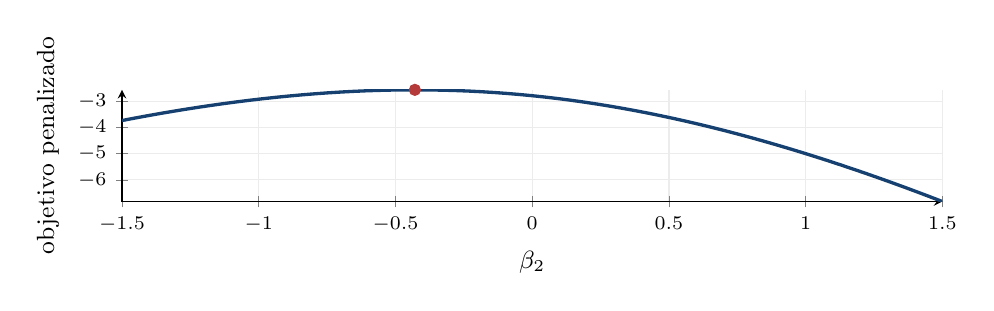
\begin{tikzpicture}
\begin{axis}[base,width=12cm,height=3cm,xmin=-1.5,xmax=1.5,xlabel={$\beta_2$},ylabel={objetivo penalizado}]
\addplot[azul,very thick] coordinates {(-1.50000,-3.73104639) (-1.45312,-3.63757270) (-1.40625,-3.54744592) (-1.35938,-3.46072646) (-1.31250,-3.37747772) (-1.26562,-3.29776617) (-1.21875,-3.22166141) (-1.17188,-3.14923613) (-1.12500,-3.08056614) (-1.07812,-3.01573032) (-1.03125,-2.95481049) (-0.98438,-2.89789129) (-0.93750,-2.84505997) (-0.89062,-2.79640612) (-0.84375,-2.75202136) (-0.79688,-2.71199888) (-0.75000,-2.67643302) (-0.70312,-2.64541863) (-0.65625,-2.61905050) (-0.60938,-2.59742256) (-0.56250,-2.58062715) (-0.51562,-2.56875410) (-0.46875,-2.56188985) (-0.42188,-2.56011651) (-0.37500,-2.56351086) (-0.32812,-2.57214342) (-0.28125,-2.58607751) (-0.23438,-2.60536841) (-0.18750,-2.63006251) (-0.14062,-2.66019668) (-0.09375,-2.69579768) (-0.04688,-2.73688177) (0.00000,-2.78345449) (0.04688,-2.83551055) (0.09375,-2.89303392) (0.14062,-2.95599815) (0.18750,-3.02436677) (0.23438,-3.09809386) (0.28125,-3.17712475) (0.32812,-3.26139683) (0.37500,-3.35084044) (0.42188,-3.44537975) (0.46875,-3.54493378) (0.51562,-3.64941728) (0.56250,-3.75874174) (0.60938,-3.87281624) (0.65625,-3.99154830) (0.70312,-4.11484467) (0.75000,-4.24261205) (0.79688,-4.37475765) (0.84375,-4.51118983) (0.89062,-4.65181851) (0.93750,-4.79655556) (0.98438,-4.94531516) (1.03125,-5.09801401) (1.07812,-5.25457154) (1.12500,-5.41491007) (1.17188,-5.57895484) (1.21875,-5.74663413) (1.26562,-5.91787921) (1.31250,-6.09262436) (1.35938,-6.27080681) (1.40625,-6.45236671) (1.45312,-6.63724700) (1.50000,-6.82539338)};\addplot[rojo,only marks,mark=*] coordinates {(-0.42912255,-2.56005483)};
\end{axis}
\end{tikzpicture}
\caption{Objetivo penalizado al mover \(\beta_2\), fijando \(\beta_1\) en su solución para esta muestra.}
\end{figure}

La suma de los dieciséis aportes forma los momentos finitos.
Una muestra con baja probabilidad tiene menos peso,
aunque sus coeficientes puedan ser de magnitud grande.
La gráfica es un corte de la función de dos variables;
mantiene fijo el intercepto, y no es un perfil reoptimizado.
\endgroup

\clearpage
\section{Muestra 1011: raíz penalizada y aporte a los momentos}\label{logit136}
\begingroup\small
\setlength{\abovedisplayskip}{4pt}\setlength{\belowdisplayskip}{4pt}
Se mantienen las cuatro filas del experimento y se observa
la siguiente configuración de respuestas:
\[
y=\begin{pmatrix}1\\0\\1\\1\end{pmatrix},\quad \Prob(Y=y\mid X)=\frac{1}{3}\cdot\frac{1}{2}\cdot\frac{2}{3}\cdot\frac{4}{5}=\frac{4}{45}.
\]

El conteo de unos y el producto con el segundo regresor son
\[
\sum_{i=1}^4 y_i=3,\qquad\sum_{i=1}^4x_{i2}y_i=(-1)(1)+0(0)+1(1)+2(1)=2.
\]

En las ecuaciones abiertas de la unidad anterior se sustituyen
estos dos resultados. En el inicio, el sistema produce
\[
\begin{pmatrix}2&1/2\\1/2&5/2\end{pmatrix}\Delta^{(0)}=\begin{pmatrix}1\\1\end{pmatrix},\qquad\Delta^{(0)}=\begin{pmatrix}0.42105263\\0.31578947\end{pmatrix}.
\]

Se recalculan probabilidades y curvatura hasta resolver
ambas ecuaciones. La solución y el objetivo penalizado son
\[
\widehat\beta(y)\approx\begin{pmatrix}0.43370094\\0.33703771\end{pmatrix},\qquad \ell(\widehat\beta(y))-\tfrac12\|\widehat\beta(y)\|_2^2\approx-2.3958195269.
\]

La sustitución final en cada fila permite verificar
los dos gradientes, incluyendo el término de penalización.
\begin{center}\scriptsize
\begin{tabular}{rrrrrrr}\toprule
\(i\)&\(x_{i2}\)&\(y_i\)&\(\widehat\beta_1+x_{i2}\widehat\beta_2\)&probabilidad&discrepancia&varianza\\\midrule
1&-1&1&0.09666323&0.52414701&0.47585299&0.24941692\\
2&0&0&0.43370094&0.60675707&-0.60675707&0.23860293\\
3&1&1&0.77073865&0.68368066&0.31631934&0.21626142\\
4&2&1&1.10777635&0.75171432&0.24828568&0.18663990\\
\\\bottomrule\end{tabular}\end{center}
La suma de discrepancias coincide con \(\widehat\beta_1\).
La suma de \(x_{i2}\) por discrepancia coincide con
\(\widehat\beta_2\). Los residuos de ambas ecuaciones
tienen valor absoluto menor que \(10^{-10}\).

La curvatura positiva penalizada en la raíz es
\[
\begin{pmatrix}1.89092117&0.34012429\\0.34012429&2.21223794\end{pmatrix}.
\]

La muestra aporta a la esperanza su probabilidad
multiplicada por el vector de coeficientes:
\[
\frac{4}{45}\,\begin{pmatrix}0.43370094\\0.33703771\end{pmatrix}=\begin{pmatrix}0.03855119\\0.02995891\end{pmatrix}.
\]

A los segundos momentos aporta esa misma probabilidad
por todos los productos de coeficientes, incluidos los cruzados:
\[
\frac{4}{45}\,\begin{pmatrix}0.18809651&0.14617357\\0.14617357&0.11359442\end{pmatrix}.
\]

\begin{figure}[H]\centering
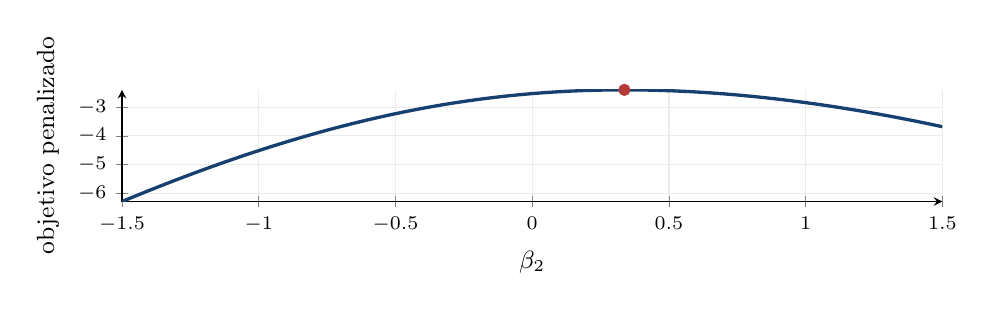
\begin{tikzpicture}
\begin{axis}[base,width=12cm,height=3cm,xmin=-1.5,xmax=1.5,xlabel={$\beta_2$},ylabel={objetivo penalizado}]
\addplot[azul,very thick] coordinates {(-1.50000,-6.28991023) (-1.45312,-6.10531936) (-1.40625,-5.92423588) (-1.35938,-5.74672940) (-1.31250,-5.57287271) (-1.26562,-5.40274175) (-1.21875,-5.23641555) (-1.17188,-5.07397612) (-1.12500,-4.91550831) (-1.07812,-4.76109952) (-1.03125,-4.61083952) (-0.98438,-4.46481997) (-0.93750,-4.32313411) (-0.89062,-4.18587611) (-0.84375,-4.05314061) (-0.79688,-3.92502193) (-0.75000,-3.80161338) (-0.70312,-3.68300644) (-0.65625,-3.56928984) (-0.60938,-3.46054868) (-0.56250,-3.35686345) (-0.51562,-3.25830907) (-0.46875,-3.16495400) (-0.42188,-3.07685925) (-0.37500,-2.99407765) (-0.32812,-2.91665302) (-0.28125,-2.84461963) (-0.23438,-2.77800164) (-0.18750,-2.71681283) (-0.14062,-2.66105640) (-0.09375,-2.61072501) (-0.04688,-2.56580091) (0.00000,-2.52625631) (0.04688,-2.49205388) (0.09375,-2.46314734) (0.14062,-2.43948222) (0.18750,-2.42099669) (0.23438,-2.40762243) (0.28125,-2.39928553) (0.32812,-2.39590749) (0.37500,-2.39740608) (0.42188,-2.40369627) (0.46875,-2.41469107) (0.51562,-2.43030231) (0.56250,-2.45044136) (0.60938,-2.47501980) (0.65625,-2.50394994) (0.70312,-2.53714536) (0.75000,-2.57452125) (0.79688,-2.61599483) (0.84375,-2.66148556) (0.89062,-2.71091537) (0.93750,-2.76420879) (0.98438,-2.82129308) (1.03125,-2.88209827) (1.07812,-2.94655718) (1.12500,-3.01460541) (1.17188,-3.08618134) (1.21875,-3.16122601) (1.26562,-3.23968311) (1.31250,-3.32149888) (1.35938,-3.40662200) (1.40625,-3.49500352) (1.45312,-3.58659676) (1.50000,-3.68135719)};\addplot[rojo,only marks,mark=*] coordinates {(0.33703771,-2.39581953)};
\end{axis}
\end{tikzpicture}
\caption{Objetivo penalizado al mover \(\beta_2\), fijando \(\beta_1\) en su solución para esta muestra.}
\end{figure}

La suma de los dieciséis aportes forma los momentos finitos.
Una muestra con baja probabilidad tiene menos peso,
aunque sus coeficientes puedan ser de magnitud grande.
La gráfica es un corte de la función de dos variables;
mantiene fijo el intercepto, y no es un perfil reoptimizado.
\endgroup

\clearpage
\section{Muestra 1100: raíz penalizada y aporte a los momentos}\label{logit137}
\begingroup\small
\setlength{\abovedisplayskip}{4pt}\setlength{\belowdisplayskip}{4pt}
Se mantienen las cuatro filas del experimento y se observa
la siguiente configuración de respuestas:
\[
y=\begin{pmatrix}1\\1\\0\\0\end{pmatrix},\quad \Prob(Y=y\mid X)=\frac{1}{3}\cdot\frac{1}{2}\cdot\frac{1}{3}\cdot\frac{1}{5}=\frac{1}{90}.
\]

El conteo de unos y el producto con el segundo regresor son
\[
\sum_{i=1}^4 y_i=2,\qquad\sum_{i=1}^4x_{i2}y_i=(-1)(1)+0(1)+1(0)+2(0)=-1.
\]

En las ecuaciones abiertas de la unidad anterior se sustituyen
estos dos resultados. En el inicio, el sistema produce
\[
\begin{pmatrix}2&1/2\\1/2&5/2\end{pmatrix}\Delta^{(0)}=\begin{pmatrix}0\\-2\end{pmatrix},\qquad\Delta^{(0)}=\begin{pmatrix}0.21052632\\-0.84210526\end{pmatrix}.
\]

Se recalculan probabilidades y curvatura hasta resolver
ambas ecuaciones. La solución y el objetivo penalizado son
\[
\widehat\beta(y)\approx\begin{pmatrix}0.20166132\\-0.90918141\end{pmatrix},\qquad \ell(\widehat\beta(y))-\tfrac12\|\widehat\beta(y)\|_2^2\approx-1.8974805320.
\]

La sustitución final en cada fila permite verificar
los dos gradientes, incluyendo el término de penalización.
\begin{center}\scriptsize
\begin{tabular}{rrrrrrr}\toprule
\(i\)&\(x_{i2}\)&\(y_i\)&\(\widehat\beta_1+x_{i2}\widehat\beta_2\)&probabilidad&discrepancia&varianza\\\midrule
1&-1&1&1.11084273&0.75228619&0.24771381&0.18635168\\
2&0&1&0.20166132&0.55024517&0.44975483&0.24747542\\
3&1&0&-0.70752008&0.33014704&-0.33014704&0.22114997\\
4&2&0&-1.61670149&0.16566028&-0.16566028&0.13821695\\
\\\bottomrule\end{tabular}\end{center}
La suma de discrepancias coincide con \(\widehat\beta_1\).
La suma de \(x_{i2}\) por discrepancia coincide con
\(\widehat\beta_2\). Los residuos de ambas ecuaciones
tienen valor absoluto menor que \(10^{-10}\).

La curvatura positiva penalizada en la raíz es
\[
\begin{pmatrix}1.79319402&0.31123219\\0.31123219&1.96036945\end{pmatrix}.
\]

La muestra aporta a la esperanza su probabilidad
multiplicada por el vector de coeficientes:
\[
\frac{1}{90}\,\begin{pmatrix}0.20166132\\-0.90918141\end{pmatrix}=\begin{pmatrix}0.00224068\\-0.01010202\end{pmatrix}.
\]

A los segundos momentos aporta esa misma probabilidad
por todos los productos de coeficientes, incluidos los cruzados:
\[
\frac{1}{90}\,\begin{pmatrix}0.04066729&-0.18334673\\-0.18334673&0.82661083\end{pmatrix}.
\]

\begin{figure}[H]\centering
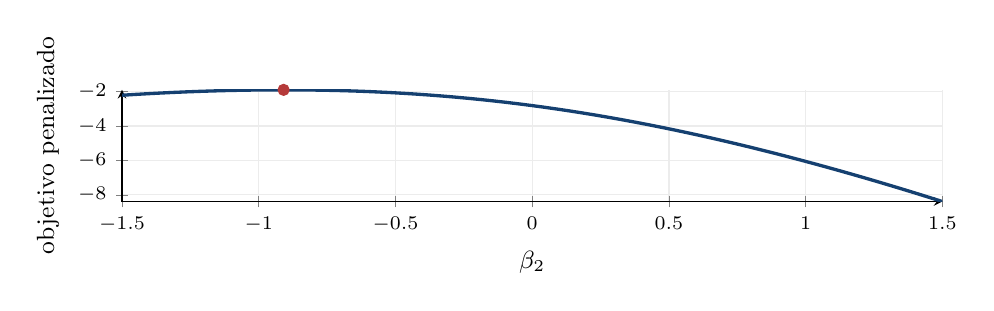
\begin{tikzpicture}
\begin{axis}[base,width=12cm,height=3cm,xmin=-1.5,xmax=1.5,xlabel={$\beta_2$},ylabel={objetivo penalizado}]
\addplot[azul,very thick] coordinates {(-1.50000,-2.21074720) (-1.45312,-2.16477450) (-1.40625,-2.12219193) (-1.35938,-2.08306267) (-1.31250,-2.04745302) (-1.26562,-2.01543240) (-1.21875,-1.98707339) (-1.17188,-1.96245172) (-1.12500,-1.94164620) (-1.07812,-1.92473863) (-1.03125,-1.91181367) (-0.98438,-1.90295861) (-0.93750,-1.89826315) (-0.89062,-1.89781902) (-0.84375,-1.90171958) (-0.79688,-1.91005936) (-0.75000,-1.92293346) (-0.70312,-1.94043692) (-0.65625,-1.96266399) (-0.60938,-1.98970733) (-0.56250,-2.02165715) (-0.51562,-2.05860027) (-0.46875,-2.10061923) (-0.42188,-2.14779125) (-0.37500,-2.20018735) (-0.32812,-2.25787136) (-0.28125,-2.32089908) (-0.23438,-2.38931748) (-0.18750,-2.46316403) (-0.14062,-2.54246613) (-0.09375,-2.62724073) (-0.04688,-2.71749408) (0.00000,-2.81322165) (0.04688,-2.91440823) (0.09375,-3.02102822) (0.14062,-3.13304604) (0.18750,-3.25041672) (0.23438,-3.37308660) (0.28125,-3.50099410) (0.32812,-3.63407061) (0.37500,-3.77224142) (0.42188,-3.91542668) (0.46875,-4.06354232) (0.51562,-4.21650098) (0.56250,-4.37421291) (0.60938,-4.53658683) (0.65625,-4.70353065) (0.70312,-4.87495222) (0.75000,-5.05075989) (0.79688,-5.23086311) (0.84375,-5.41517286) (0.89062,-5.60360206) (0.93750,-5.79606582) (0.98438,-5.99248180) (1.03125,-6.19277028) (1.07812,-6.39685438) (1.12500,-6.60466010) (1.17188,-6.81611639) (1.21875,-7.03115514) (1.26562,-7.24971118) (1.31250,-7.47172224) (1.35938,-7.69712888) (1.40625,-7.92587441) (1.45312,-8.15790483) (1.50000,-8.39316870)};\addplot[rojo,only marks,mark=*] coordinates {(-0.90918141,-1.89748053)};
\end{axis}
\end{tikzpicture}
\caption{Objetivo penalizado al mover \(\beta_2\), fijando \(\beta_1\) en su solución para esta muestra.}
\end{figure}

La suma de los dieciséis aportes forma los momentos finitos.
Una muestra con baja probabilidad tiene menos peso,
aunque sus coeficientes puedan ser de magnitud grande.
La gráfica es un corte de la función de dos variables;
mantiene fijo el intercepto, y no es un perfil reoptimizado.
\endgroup

\clearpage
\section{Muestra 1101: raíz penalizada y aporte a los momentos}\label{logit138}
\begingroup\small
\setlength{\abovedisplayskip}{4pt}\setlength{\belowdisplayskip}{4pt}
Se mantienen las cuatro filas del experimento y se observa
la siguiente configuración de respuestas:
\[
y=\begin{pmatrix}1\\1\\0\\1\end{pmatrix},\quad \Prob(Y=y\mid X)=\frac{1}{3}\cdot\frac{1}{2}\cdot\frac{1}{3}\cdot\frac{4}{5}=\frac{2}{45}.
\]

El conteo de unos y el producto con el segundo regresor son
\[
\sum_{i=1}^4 y_i=3,\qquad\sum_{i=1}^4x_{i2}y_i=(-1)(1)+0(1)+1(0)+2(1)=1.
\]

En las ecuaciones abiertas de la unidad anterior se sustituyen
estos dos resultados. En el inicio, el sistema produce
\[
\begin{pmatrix}2&1/2\\1/2&5/2\end{pmatrix}\Delta^{(0)}=\begin{pmatrix}1\\0\end{pmatrix},\qquad\Delta^{(0)}=\begin{pmatrix}0.52631579\\-0.10526316\end{pmatrix}.
\]

Se recalculan probabilidades y curvatura hasta resolver
ambas ecuaciones. La solución y el objetivo penalizado son
\[
\widehat\beta(y)\approx\begin{pmatrix}0.53209600\\-0.10735785\end{pmatrix},\qquad \ell(\widehat\beta(y))-\tfrac12\|\widehat\beta(y)\|_2^2\approx-2.5079860843.
\]

La sustitución final en cada fila permite verificar
los dos gradientes, incluyendo el término de penalización.
\begin{center}\scriptsize
\begin{tabular}{rrrrrrr}\toprule
\(i\)&\(x_{i2}\)&\(y_i\)&\(\widehat\beta_1+x_{i2}\widehat\beta_2\)&probabilidad&discrepancia&varianza\\\midrule
1&-1&1&0.63945385&0.65462999&0.34537001&0.22608957\\
2&0&1&0.53209600&0.62997184&0.37002816&0.23310732\\
3&1&0&0.42473815&0.60461649&-0.60461649&0.23905539\\
4&2&1&0.31738030&0.57868568&0.42131432&0.24380856\\
\\\bottomrule\end{tabular}\end{center}
La suma de discrepancias coincide con \(\widehat\beta_1\).
La suma de \(x_{i2}\) por discrepancia coincide con
\(\widehat\beta_2\). Los residuos de ambas ecuaciones
tienen valor absoluto menor que \(10^{-10}\).

La curvatura positiva penalizada en la raíz es
\[
\begin{pmatrix}1.94206084&0.50058295\\0.50058295&2.44037921\end{pmatrix}.
\]

La muestra aporta a la esperanza su probabilidad
multiplicada por el vector de coeficientes:
\[
\frac{2}{45}\,\begin{pmatrix}0.53209600\\-0.10735785\end{pmatrix}=\begin{pmatrix}0.02364871\\-0.00477146\end{pmatrix}.
\]

A los segundos momentos aporta esa misma probabilidad
por todos los productos de coeficientes, incluidos los cruzados:
\[
\frac{2}{45}\,\begin{pmatrix}0.28312615&-0.05712468\\-0.05712468&0.01152571\end{pmatrix}.
\]

\begin{figure}[H]\centering
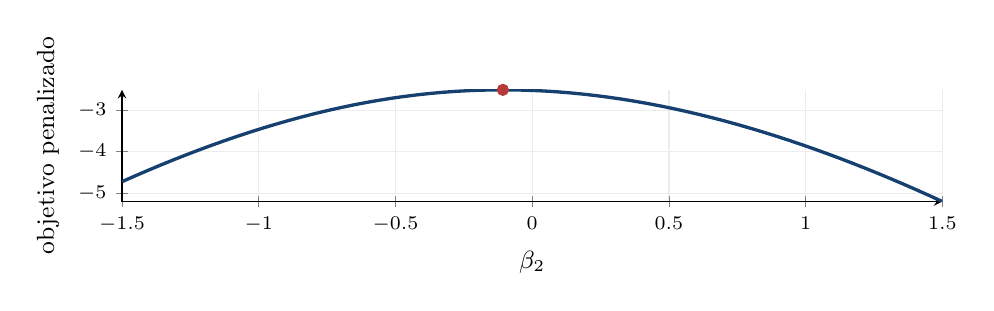
\begin{tikzpicture}
\begin{axis}[base,width=12cm,height=3cm,xmin=-1.5,xmax=1.5,xlabel={$\beta_2$},ylabel={objetivo penalizado}]
\addplot[azul,very thick] coordinates {(-1.50000,-4.72305927) (-1.45312,-4.58641681) (-1.40625,-4.45333747) (-1.35938,-4.32389342) (-1.31250,-4.19815997) (-1.26562,-4.07621553) (-1.21875,-3.95814146) (-1.17188,-3.84402196) (-1.12500,-3.73394381) (-1.07812,-3.62799611) (-1.03125,-3.52626988) (-0.98438,-3.42885770) (-0.93750,-3.33585310) (-0.89062,-3.24735007) (-0.84375,-3.16344228) (-0.79688,-3.08422241) (-0.75000,-3.00978131) (-0.70312,-2.94020710) (-0.65625,-2.87558427) (-0.60938,-2.81599274) (-0.56250,-2.76150689) (-0.51562,-2.71219462) (-0.46875,-2.66811651) (-0.42188,-2.62932492) (-0.37500,-2.59586333) (-0.32812,-2.56776569) (-0.28125,-2.54505594) (-0.23438,-2.52774773) (-0.18750,-2.51584422) (-0.14062,-2.50933813) (-0.09375,-2.50821191) (-0.04688,-2.51243807) (0.00000,-2.52197973) (0.04688,-2.53679116) (0.09375,-2.55681862) (0.14062,-2.58200111) (0.18750,-2.61227125) (0.23438,-2.64755627) (0.28125,-2.68777887) (0.32812,-2.73285815) (0.37500,-2.78271052) (0.42188,-2.83725051) (0.46875,-2.89639156) (0.51562,-2.96004674) (0.56250,-3.02812935) (0.60938,-3.10055350) (0.65625,-3.17723456) (0.70312,-3.25808959) (0.75000,-3.34303763) (0.79688,-3.43199998) (0.84375,-3.52490040) (0.89062,-3.62166521) (0.93750,-3.72222343) (0.98438,-3.82650681) (1.03125,-3.93444984) (1.07812,-4.04598971) (1.12500,-4.16106635) (1.17188,-4.27962226) (1.21875,-4.40160252) (1.26562,-4.52695468) (1.31250,-4.65562864) (1.35938,-4.78757661) (1.40625,-4.92275295) (1.45312,-5.06111410) (1.50000,-5.20261848)};\addplot[rojo,only marks,mark=*] coordinates {(-0.10735785,-2.50798608)};
\end{axis}
\end{tikzpicture}
\caption{Objetivo penalizado al mover \(\beta_2\), fijando \(\beta_1\) en su solución para esta muestra.}
\end{figure}

La suma de los dieciséis aportes forma los momentos finitos.
Una muestra con baja probabilidad tiene menos peso,
aunque sus coeficientes puedan ser de magnitud grande.
La gráfica es un corte de la función de dos variables;
mantiene fijo el intercepto, y no es un perfil reoptimizado.
\endgroup

\clearpage
\section{Muestra 1110: raíz penalizada y aporte a los momentos}\label{logit139}
\begingroup\small
\setlength{\abovedisplayskip}{4pt}\setlength{\belowdisplayskip}{4pt}
Se mantienen las cuatro filas del experimento y se observa
la siguiente configuración de respuestas:
\[
y=\begin{pmatrix}1\\1\\1\\0\end{pmatrix},\quad \Prob(Y=y\mid X)=\frac{1}{3}\cdot\frac{1}{2}\cdot\frac{2}{3}\cdot\frac{1}{5}=\frac{1}{45}.
\]

El conteo de unos y el producto con el segundo regresor son
\[
\sum_{i=1}^4 y_i=3,\qquad\sum_{i=1}^4x_{i2}y_i=(-1)(1)+0(1)+1(1)+2(0)=0.
\]

En las ecuaciones abiertas de la unidad anterior se sustituyen
estos dos resultados. En el inicio, el sistema produce
\[
\begin{pmatrix}2&1/2\\1/2&5/2\end{pmatrix}\Delta^{(0)}=\begin{pmatrix}1\\-1\end{pmatrix},\qquad\Delta^{(0)}=\begin{pmatrix}0.63157895\\-0.52631579\end{pmatrix}.
\]

Se recalculan probabilidades y curvatura hasta resolver
ambas ecuaciones. La solución y el objetivo penalizado son
\[
\widehat\beta(y)\approx\begin{pmatrix}0.65380458\\-0.54464644\end{pmatrix},\qquad \ell(\widehat\beta(y))-\tfrac12\|\widehat\beta(y)\|_2^2\approx-2.1834244560.
\]

La sustitución final en cada fila permite verificar
los dos gradientes, incluyendo el término de penalización.
\begin{center}\scriptsize
\begin{tabular}{rrrrrrr}\toprule
\(i\)&\(x_{i2}\)&\(y_i\)&\(\widehat\beta_1+x_{i2}\widehat\beta_2\)&probabilidad&discrepancia&varianza\\\midrule
1&-1&1&1.19845101&0.76824911&0.23175089&0.17804241\\
2&0&1&0.65380458&0.65786730&0.34213270&0.22507791\\
3&1&1&0.10915814&0.52726247&0.47273753&0.24925676\\
4&2&0&-0.43548830&0.39281654&-0.39281654&0.23851171\\
\\\bottomrule\end{tabular}\end{center}
La suma de discrepancias coincide con \(\widehat\beta_1\).
La suma de \(x_{i2}\) por discrepancia coincide con
\(\widehat\beta_2\). Los residuos de ambas ecuaciones
tienen valor absoluto menor que \(10^{-10}\).

La curvatura positiva penalizada en la raíz es
\[
\begin{pmatrix}1.89088879&0.54823776\\0.54823776&2.38134600\end{pmatrix}.
\]

La muestra aporta a la esperanza su probabilidad
multiplicada por el vector de coeficientes:
\[
\frac{1}{45}\,\begin{pmatrix}0.65380458\\-0.54464644\end{pmatrix}=\begin{pmatrix}0.01452899\\-0.01210325\end{pmatrix}.
\]

A los segundos momentos aporta esa misma probabilidad
por todos los productos de coeficientes, incluidos los cruzados:
\[
\frac{1}{45}\,\begin{pmatrix}0.42746042&-0.35609233\\-0.35609233&0.29663974\end{pmatrix}.
\]

\begin{figure}[H]\centering
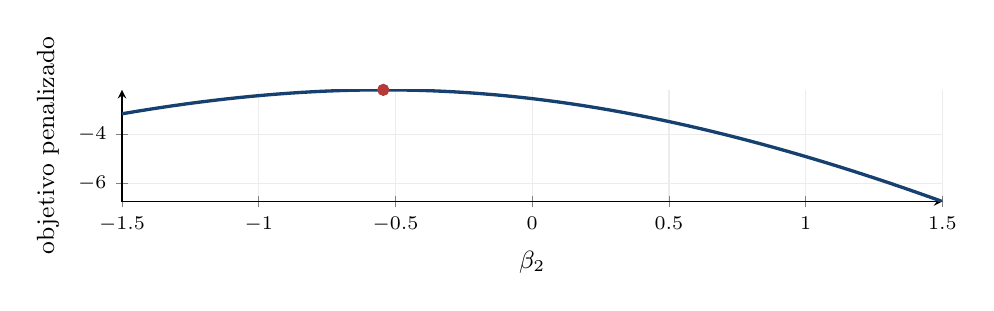
\begin{tikzpicture}
\begin{axis}[base,width=12cm,height=3cm,xmin=-1.5,xmax=1.5,xlabel={$\beta_2$},ylabel={objetivo penalizado}]
\addplot[azul,very thick] coordinates {(-1.50000,-3.16189508) (-1.45312,-3.07363971) (-1.40625,-2.98902104) (-1.35938,-2.90811421) (-1.31250,-2.83099740) (-1.26562,-2.75775173) (-1.21875,-2.68846104) (-1.17188,-2.62321171) (-1.12500,-2.56209231) (-1.07812,-2.50519326) (-1.03125,-2.45260635) (-0.98438,-2.40442426) (-0.93750,-2.36073986) (-0.89062,-2.32164562) (-0.84375,-2.28723277) (-0.79688,-2.25759052) (-0.75000,-2.23280514) (-0.70312,-2.21295907) (-0.65625,-2.19812993) (-0.60938,-2.18838966) (-0.56250,-2.18380351) (-0.51562,-2.18442924) (-0.46875,-2.19031630) (-0.42188,-2.20150515) (-0.37500,-2.21802670) (-0.32812,-2.23990184) (-0.28125,-2.26714126) (-0.23438,-2.29974526) (-0.18750,-2.33770388) (-0.14062,-2.38099712) (-0.09375,-2.42959529) (-0.04688,-2.48345964) (0.00000,-2.54254293) (0.04688,-2.60679026) (0.09375,-2.67613985) (0.14062,-2.75052399) (0.18750,-2.82986995) (0.23438,-2.91410084) (0.28125,-3.00313660) (0.32812,-3.09689481) (0.37500,-3.19529150) (0.42188,-3.29824195) (0.46875,-3.40566129) (0.51562,-3.51746515) (0.56250,-3.63357017) (0.60938,-3.75389443) (0.65625,-3.87835782) (0.70312,-4.00688233) (0.75000,-4.13939226) (0.79688,-4.27581443) (0.84375,-4.41607825) (0.89062,-4.56011581) (0.93750,-4.70786190) (0.98438,-4.85925399) (1.03125,-5.01423224) (1.07812,-5.17273940) (1.12500,-5.33472075) (1.17188,-5.50012402) (1.21875,-5.66889931) (1.26562,-5.84099896) (1.31250,-6.01637746) (1.35938,-6.19499136) (1.40625,-6.37679912) (1.45312,-6.56176108) (1.50000,-6.74983929)};\addplot[rojo,only marks,mark=*] coordinates {(-0.54464644,-2.18342446)};
\end{axis}
\end{tikzpicture}
\caption{Objetivo penalizado al mover \(\beta_2\), fijando \(\beta_1\) en su solución para esta muestra.}
\end{figure}

La suma de los dieciséis aportes forma los momentos finitos.
Una muestra con baja probabilidad tiene menos peso,
aunque sus coeficientes puedan ser de magnitud grande.
La gráfica es un corte de la función de dos variables;
mantiene fijo el intercepto, y no es un perfil reoptimizado.
\endgroup

\clearpage
\section{Muestra 1111: raíz penalizada y aporte a los momentos}\label{logit140}
\begingroup\small
\setlength{\abovedisplayskip}{4pt}\setlength{\belowdisplayskip}{4pt}
Se mantienen las cuatro filas del experimento y se observa
la siguiente configuración de respuestas:
\[
y=\begin{pmatrix}1\\1\\1\\1\end{pmatrix},\quad \Prob(Y=y\mid X)=\frac{1}{3}\cdot\frac{1}{2}\cdot\frac{2}{3}\cdot\frac{4}{5}=\frac{4}{45}.
\]

El conteo de unos y el producto con el segundo regresor son
\[
\sum_{i=1}^4 y_i=4,\qquad\sum_{i=1}^4x_{i2}y_i=(-1)(1)+0(1)+1(1)+2(1)=2.
\]

En las ecuaciones abiertas de la unidad anterior se sustituyen
estos dos resultados. En el inicio, el sistema produce
\[
\begin{pmatrix}2&1/2\\1/2&5/2\end{pmatrix}\Delta^{(0)}=\begin{pmatrix}2\\1\end{pmatrix},\qquad\Delta^{(0)}=\begin{pmatrix}0.94736842\\0.21052632\end{pmatrix}.
\]

Se recalculan probabilidades y curvatura hasta resolver
ambas ecuaciones. La solución y el objetivo penalizado son
\[
\widehat\beta(y)\approx\begin{pmatrix}0.99575846\\0.25896422\end{pmatrix},\qquad \ell(\widehat\beta(y))-\tfrac12\|\widehat\beta(y)\|_2^2\approx-1.6846392328.
\]

La sustitución final en cada fila permite verificar
los dos gradientes, incluyendo el término de penalización.
\begin{center}\scriptsize
\begin{tabular}{rrrrrrr}\toprule
\(i\)&\(x_{i2}\)&\(y_i\)&\(\widehat\beta_1+x_{i2}\widehat\beta_2\)&probabilidad&discrepancia&varianza\\\midrule
1&-1&1&0.73679424&0.67629445&0.32370555&0.21892027\\
2&0&1&0.99575846&0.73022382&0.26977618&0.19699699\\
3&1&1&1.25472268&0.77811631&0.22188369&0.17265132\\
4&2&1&1.51368689&0.81960696&0.18039304&0.14785139\\
\\\bottomrule\end{tabular}\end{center}
La suma de discrepancias coincide con \(\widehat\beta_1\).
La suma de \(x_{i2}\) por discrepancia coincide con
\(\widehat\beta_2\). Los residuos de ambas ecuaciones
tienen valor absoluto menor que \(10^{-10}\).

La curvatura positiva penalizada en la raíz es
\[
\begin{pmatrix}1.73641997&0.24943383\\0.24943383&1.98297715\end{pmatrix}.
\]

La muestra aporta a la esperanza su probabilidad
multiplicada por el vector de coeficientes:
\[
\frac{4}{45}\,\begin{pmatrix}0.99575846\\0.25896422\end{pmatrix}=\begin{pmatrix}0.08851186\\0.02301904\end{pmatrix}.
\]

A los segundos momentos aporta esa misma probabilidad
por todos los productos de coeficientes, incluidos los cruzados:
\[
\frac{4}{45}\,\begin{pmatrix}0.99153491&0.25786581\\0.25786581&0.06706247\end{pmatrix}.
\]

\begin{figure}[H]\centering
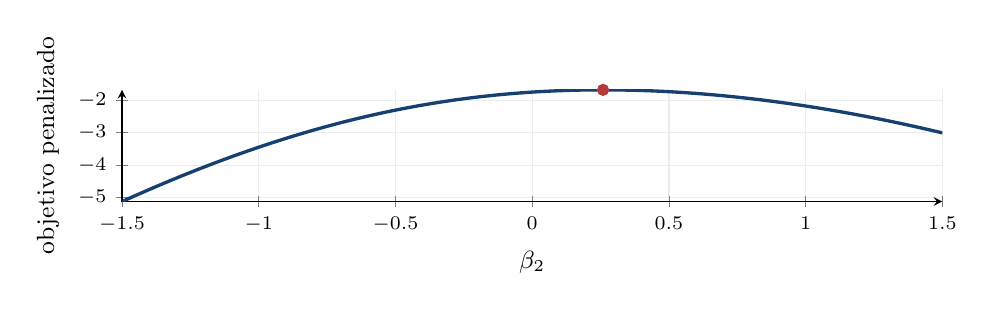
\begin{tikzpicture}
\begin{axis}[base,width=12cm,height=3cm,xmin=-1.5,xmax=1.5,xlabel={$\beta_2$},ylabel={objetivo penalizado}]
\addplot[azul,very thick] coordinates {(-1.50000,-5.12176793) (-1.45312,-4.94509120) (-1.40625,-4.77228139) (-1.35938,-4.60342021) (-1.31250,-4.43859165) (-1.26562,-4.27788162) (-1.21875,-4.12137758) (-1.17188,-3.96916799) (-1.12500,-3.82134182) (-1.07812,-3.67798782) (-1.03125,-3.53919391) (-0.98438,-3.40504627) (-0.93750,-3.27562861) (-0.89062,-3.15102120) (-0.84375,-3.03129999) (-0.79688,-2.91653568) (-0.75000,-2.80679284) (-0.70312,-2.70212899) (-0.65625,-2.60259385) (-0.60938,-2.50822864) (-0.56250,-2.41906543) (-0.51562,-2.33512675) (-0.46875,-2.25642526) (-0.42188,-2.18296360) (-0.37500,-2.11473443) (-0.32812,-2.05172062) (-0.28125,-1.99389560) (-0.23438,-1.94122387) (-0.18750,-1.89366162) (-0.14062,-1.85115748) (-0.09375,-1.81365334) (-0.04688,-1.78108522) (0.00000,-1.75338419) (0.04688,-1.73047729) (0.09375,-1.71228845) (0.14062,-1.69873934) (0.18750,-1.68975021) (0.23438,-1.68524064) (0.28125,-1.68513023) (0.32812,-1.68933922) (0.37500,-1.69778899) (0.42188,-1.71040251) (0.46875,-1.72710475) (0.51562,-1.74782291) (0.56250,-1.77248668) (0.60938,-1.80102838) (0.65625,-1.83338307) (0.70312,-1.86948862) (0.75000,-1.90928567) (0.79688,-1.95271766) (0.84375,-1.99973071) (0.89062,-2.05027362) (0.93750,-2.10429769) (0.98438,-2.16175667) (1.03125,-2.22260660) (1.07812,-2.28680570) (1.12500,-2.35431425) (1.17188,-2.42509441) (1.21875,-2.49911018) (1.26562,-2.57632717) (1.31250,-2.65671256) (1.35938,-2.74023496) (1.40625,-2.82686429) (1.45312,-2.91657169) (1.50000,-3.00932942)};\addplot[rojo,only marks,mark=*] coordinates {(0.25896422,-1.68463923)};
\end{axis}
\end{tikzpicture}
\caption{Objetivo penalizado al mover \(\beta_2\), fijando \(\beta_1\) en su solución para esta muestra.}
\end{figure}

La suma de los dieciséis aportes forma los momentos finitos.
Una muestra con baja probabilidad tiene menos peso,
aunque sus coeficientes puedan ser de magnitud grande.
La gráfica es un corte de la función de dos variables;
mantiene fijo el intercepto, y no es un perfil reoptimizado.
\endgroup

\clearpage
\section{Esperanza finita de las dos coordenadas: sumar las dieciséis raíces}\label{logit141}
\begingroup\small
La esperanza condicionada en este diseño es una suma
sobre todas las respuestas posibles.
El diseño y el parámetro verdadero determinan las probabilidades
de las muestras; la regla penalizada determina la raíz en cada una.
Para cada coordenada,
\[
\E[\widehat\beta_j(Y)\mid X]
=\sum_{y\in\{0,1\}^4}\Prob(Y=y\mid X)\widehat\beta_j(y).
\]
No se evalúa una sola raíz en la respuesta esperada.
Como la raíz es una función no lineal,
esa sustitución no produciría en general la esperanza.

Las dieciséis masas suman uno exactamente:
\[
\sum_{y\in\{0,1\}^4}\Prob(Y=y\mid X)
=\prod_{i=1}^4[\Prob(Y_i=0\mid X)+\Prob(Y_i=1\mid X)]=1.
\]
La tabla muestra cada factor de la suma y sus productos.
\begin{center}\scriptsize
\begin{tabular}{crrrrr}\toprule
\(y_1y_2y_3y_4\)&masa&\(\widehat\beta_1(y)\)&\(\widehat\beta_2(y)\)&aporte a \(\E[\widehat\beta_1]\)&aporte a \(\E[\widehat\beta_2]\)\\\midrule
0000&$\frac{1}{45}$&-0.99575846&-0.25896422&-0.02212797&-0.00575476\\
0001&$\frac{4}{45}$&-0.65380458&0.54464644&-0.05811596&0.04841302\\
0010&$\frac{2}{45}$&-0.53209600&0.10735785&-0.02364871&0.00477146\\
0011&$\frac{8}{45}$&-0.20166132&0.90918141&-0.03585090&0.16163225\\
0100&$\frac{1}{45}$&-0.43370094&-0.33703771&-0.00963780&-0.00748973\\
0101&$\frac{4}{45}$&-0.10425081&0.42912255&-0.00926674&0.03814423\\
0110&$\frac{2}{45}$&0.00000000&0.00000000&0.00000000&0.00000000\\
0111&$\frac{8}{45}$&0.36856083&0.84144532&0.06552193&0.14959028\\
1000&$\frac{1}{90}$&-0.36856083&-0.84144532&-0.00409512&-0.00934939\\
1001&$\frac{2}{45}$&0.00000000&0.00000000&0.00000000&0.00000000\\
1010&$\frac{1}{45}$&0.10425081&-0.42912255&0.00231668&-0.00953606\\
1011&$\frac{4}{45}$&0.43370094&0.33703771&0.03855119&0.02995891\\
1100&$\frac{1}{90}$&0.20166132&-0.90918141&0.00224068&-0.01010202\\
1101&$\frac{2}{45}$&0.53209600&-0.10735785&0.02364871&-0.00477146\\
1110&$\frac{1}{45}$&0.65380458&-0.54464644&0.01452899&-0.01210325\\
1111&$\frac{4}{45}$&0.99575846&0.25896422&0.08851186&0.02301904\\
\\\bottomrule\end{tabular}\end{center}
Al sumar las dos columnas de aportes, conservando más
cifras internas que las impresas, se obtiene
\[
\begin{aligned}
\E[\widehat\beta_1\mid X]&\approx(-0.0221280)+(-0.0581160)+(-0.0236487)+(-0.0358509)\\&\quad+(-0.0096378)+(-0.0092667)+(0.0000000)+(0.0655219)\\&\quad+(-0.0040951)+(0.0000000)+(0.0023167)+(0.0385512)\\&\quad+(0.0022407)+(0.0236487)+(0.0145290)+(0.0885119)\\&=0.0725768524,\\\E[\widehat\beta_2\mid X]&\approx(-0.0057548)+(0.0484130)+(0.0047715)+(0.1616323)\\&\quad+(-0.0074897)+(0.0381442)+(0.0000000)+(0.1495903)\\&\quad+(-0.0093494)+(0.0000000)+(-0.0095361)+(0.0299589)\\&\quad+(-0.0101020)+(-0.0047715)+(-0.0121033)+(0.0230190)\\&=0.3964225150.\end{aligned}
\]

Los valores verdaderos son cero y \(\log2\).
La diferencia entre cada media y su valor verdadero
es el sesgo finito de la regla penalizada en este experimento.
Estos números no pretenden ser la esperanza del
máximo verosímil ordinario ni un límite asintótico.
Cambiar la intensidad de penalización cambia las
dieciséis raíces y por ello cambia la esperanza.
\endgroup

\clearpage
\section{Segundos momentos: dos cuadrados y el producto cruzado}\label{logit142}
\begingroup\small
Para dos coordenadas no basta calcular por separado sus cuadrados.
La entrada cruzada del segundo momento contiene el producto
de ambas raíces calculadas con la misma respuesta.
La identidad finita es
\[
\E[\widehat\beta_j\widehat\beta_l\mid X]
=\sum_{y\in\{0,1\}^4}
\Prob(Y=y\mid X)\widehat\beta_j(y)\widehat\beta_l(y).
\]
Si se multiplicaran raíces obtenidas en muestras independientes,
se estaría calculando el producto de esperanzas,
y se perdería la covarianza que se desea estudiar.

Los dieciséis aportes a las tres entradas distintas son
\begin{center}\scriptsize
\begin{tabular}{crrrr}\toprule
\(y_1y_2y_3y_4\)&masa&aporte a \(\E[\widehat\beta_1^2]\)&aporte a \(\E[\widehat\beta_1\widehat\beta_2]\)&aporte a \(\E[\widehat\beta_2^2]\)\\\midrule
0000&$\frac{1}{45}$&0.022034109&0.005730351&0.001490277\\
0001&$\frac{4}{45}$&0.037996482&-0.031652652&0.026367977\\
0010&$\frac{2}{45}$&0.012583385&-0.002538875&0.000512254\\
0011&$\frac{8}{45}$&0.007229740&-0.032594973&0.146953037\\
0100&$\frac{1}{45}$&0.004179922&0.003248302&0.002524320\\
0101&$\frac{4}{45}$&0.000966065&-0.003976567&0.016368548\\
0110&$\frac{2}{45}$&0.000000000&0.000000000&0.000000000\\
0111&$\frac{8}{45}$&0.024148815&0.055133118&0.125872039\\
1000&$\frac{1}{90}$&0.001509301&0.003445820&0.007867002\\
1001&$\frac{2}{45}$&0.000000000&0.000000000&0.000000000\\
1010&$\frac{1}{45}$&0.000241516&-0.000994142&0.004092137\\
1011&$\frac{4}{45}$&0.016719689&0.012993206&0.010097281\\
1100&$\frac{1}{90}$&0.000451859&-0.002037186&0.009184565\\
1101&$\frac{2}{45}$&0.012583385&-0.002538875&0.000512254\\
1110&$\frac{1}{45}$&0.009499121&-0.007913163&0.006591994\\
1111&$\frac{4}{45}$&0.088136436&0.022921405&0.005961108\\
\\\bottomrule\end{tabular}\end{center}
Se suman cada una de las columnas numéricas:
\[
\begin{aligned}
\E[\widehat\beta_1\widehat\beta_1\mid X]&\approx(0.0220341)+(0.0379965)+(0.0125834)+(0.0072297)\\&\quad+(0.0041799)+(0.0009661)+(0.0000000)+(0.0241488)\\&\quad+(0.0015093)+(0.0000000)+(0.0002415)+(0.0167197)\\&\quad+(0.0004519)+(0.0125834)+(0.0094991)+(0.0881364)\\&=0.2382798256.\end{aligned}
\]
\[
\begin{aligned}
\E[\widehat\beta_1\widehat\beta_2\mid X]&\approx(0.0057304)+(-0.0316527)+(-0.0025389)+(-0.0325950)\\&\quad+(0.0032483)+(-0.0039766)+(0.0000000)+(0.0551331)\\&\quad+(0.0034458)+(0.0000000)+(-0.0009941)+(0.0129932)\\&\quad+(-0.0020372)+(-0.0025389)+(-0.0079132)+(0.0229214)\\&=0.0192257699.\end{aligned}
\]
\[
\begin{aligned}
\E[\widehat\beta_2\widehat\beta_2\mid X]&\approx(0.0014903)+(0.0263680)+(0.0005123)+(0.1469530)\\&\quad+(0.0025243)+(0.0163685)+(0.0000000)+(0.1258720)\\&\quad+(0.0078670)+(0.0000000)+(0.0040921)+(0.0100973)\\&\quad+(0.0091846)+(0.0005123)+(0.0065920)+(0.0059611)\\&=0.3643947940.\end{aligned}
\]

Reunir las entradas produce la matriz de segundos momentos
\[
\E[\widehat\beta\widehat\beta\T\mid X]\approx\begin{pmatrix}0.23827983&0.01922577\\0.01922577&0.36439479\end{pmatrix}.
\]

Esta matriz es semidefinida positiva porque para cualquier
vector \(v\) su forma cuadrática es
\(\E[(v\T\widehat\beta)^2\mid X]\ge0\).
Todavía no es la covarianza: falta restar los productos
de las medias de ambos coeficientes.
\endgroup

\clearpage
\section{Covarianza finita del estimador penalizado: restar todos los productos de medias}\label{logit143}
Por definición, la entrada \((j,l)\) de la covarianza es
\[
\E[(\widehat\beta_j-\E[\widehat\beta_j])
(\widehat\beta_l-\E[\widehat\beta_l])\mid X].
\]
Las esperanzas en esta unidad están todas condicionadas
en el mismo diseño fijo.
Expandir el producto antes de tomar esperanza da cuatro términos:
\[
\begin{aligned}
&\E[\widehat\beta_j\widehat\beta_l\mid X]
-\E[\widehat\beta_j\mid X]\E[\widehat\beta_l\mid X]\\
&-\E[\widehat\beta_l\mid X]\E[\widehat\beta_j\mid X]
+\E[\widehat\beta_j\mid X]\E[\widehat\beta_l\mid X].
\end{aligned}
\]
Los últimos tres se simplifican a un solo producto negativo.
Para las dos diagonales y la entrada cruzada,
\[
\begin{aligned}
\Cov(\widehat\beta_1,\widehat\beta_1\mid X)&\approx0.2382798256-(0.0725768524)(0.0725768524)\\&=0.2330124261.\end{aligned}
\]
\[
\begin{aligned}
\Cov(\widehat\beta_1,\widehat\beta_2\mid X)&\approx0.0192257699-(0.0725768524)(0.3964225150)\\&=-0.0095453285.\end{aligned}
\]
\[
\begin{aligned}
\Cov(\widehat\beta_2,\widehat\beta_2\mid X)&\approx0.3643947940-(0.3964225150)(0.3964225150)\\&=0.2072439836.\end{aligned}
\]

La matriz resultante es
\[
\Cov(\widehat\beta\mid X)\approx\begin{pmatrix}0.23301243&-0.00954533\\-0.00954533&0.20724398\end{pmatrix}.
\]

También se puede comprobar sumando directamente los dieciséis
productos de vectores centrados:
\[
\sum_y\Prob(Y=y\mid X)
(\widehat\beta(y)-\E[\widehat\beta\mid X])
(\widehat\beta(y)-\E[\widehat\beta\mid X])\T.
\]
Cada sumando es semidefinido positivo.
Esta representación evita restar dos cantidades grandes
cuando las varianzas son pequeñas y sirve de verificación
numérica independiente de la fórmula de segundos momentos.

Sus autovalores son aproximadamente
\[
0.2040933537,\quad0.2361630561.
\]

La positividad confirma que es una matriz de dispersión válida.
La correlación se obtiene dividiendo la covarianza cruzada
por la raíz del producto de las dos varianzas:
\[
\operatorname{Corr}(\widehat\beta_1,\widehat\beta_2\mid X)\approx-0.0434370548.
\]

Esta es una covarianza de muestra finita de una regla
de estimación que existe en todas las configuraciones.
No se calculó invirtiendo una Hessiana de una sola muestra.
Las dos operaciones contestan preguntas diferentes.

\clearpage
\section{Sesgo y error cuadrático matricial: conservar el producto exterior}\label{logit144}
El sesgo es la diferencia entre la esperanza del estimador
y el parámetro verdadero. Aquí las dos coordenadas son
\[
\E[\widehat\beta\mid X]-\beta_\star\approx\begin{pmatrix}0.07257685\\0.39642252\end{pmatrix}-\begin{pmatrix}0\\\log2\end{pmatrix}=\begin{pmatrix}0.07257685\\-0.29672467\end{pmatrix}.
\]

El error cuadrático matricial mide todos los productos
entre errores de estimación:
\[
\E[(\widehat\beta-\beta_\star)
(\widehat\beta-\beta_\star)\T\mid X].
\]
Para derivar su descomposición, escribamos
\[
\widehat\beta-\beta_\star
=(\widehat\beta-\E[\widehat\beta\mid X])
+(\E[\widehat\beta\mid X]-\beta_\star).
\]
Multiplicar esta suma por su transpuesta genera cuatro
matrices: el producto de los dos vectores centrados,
dos productos cruzados y el producto del sesgo consigo mismo.
Al tomar esperanza, los dos productos cruzados se anulan
porque la media del vector centrado es cero.
Por ello
\[
\begin{aligned}
&\E[(\widehat\beta-\beta_\star)
(\widehat\beta-\beta_\star)\T\mid X]\\
&=\Cov(\widehat\beta\mid X)
+(\E[\widehat\beta\mid X]-\beta_\star)
(\E[\widehat\beta\mid X]-\beta_\star)\T.
\end{aligned}
\]
La segunda matriz no contiene solamente cuadrados
de sesgos: sus entradas cruzadas son productos de
sesgos de coordenadas distintas.
La sustitución completa es
\[
\begin{pmatrix}0.23301243&-0.00954533\\-0.00954533&0.20724398\end{pmatrix}+\begin{pmatrix}0.00526740&-0.02153534\\-0.02153534&0.08804553\end{pmatrix}=\begin{pmatrix}0.23827983&-0.03108067\\-0.03108067&0.29528951\end{pmatrix}.
\]

La diagonal da errores cuadráticos medios de cada coeficiente.
La traza suma los dos errores y coincide con
\(\E[\|\widehat\beta-\beta_\star\|_2^2\mid X]\).
En este experimento,
\[
\E[\|\widehat\beta-\beta_\star\|_2^2\mid X]\approx0.5335693364.
\]

Una penalización fuerte puede bajar la varianza y aumentar
el sesgo. Su utilidad para error cuadrático depende de la
suma de ambas contribuciones.
La matriz de covarianza por sí sola no mide esa suma.
Tampoco la magnitud de un solo coeficiente demuestra
que su estimación sea más precisa.

\clearpage
\section{Tres intensidades de penalización: repetir la enumeración completa}\label{logit145}
El parámetro verdadero y las probabilidades de las muestras
se mantienen fijos. Cambiamos únicamente la intensidad
de penalización entre \(1/4,1,4\).
Para cada intensidad se resuelven otra vez las dieciséis
ecuaciones de estimación y se repiten las sumas de momentos.
No se transforma el resultado de intensidad uno
multiplicándolo por una constante.

Con intensidad \(\lambda\), las ecuaciones del gradiente son
\[
\sum_i x_{ij}\left[y_i-
\frac{e^{\widehat\beta_1+x_{i2}\widehat\beta_2}}
{1+e^{\widehat\beta_1+x_{i2}\widehat\beta_2}}\right]
-\lambda\widehat\beta_j=0,\qquad j=1,2.
\]
La curvatura incluye \(\lambda I_2\) y la cota de norma es
\[
\|\widehat\beta\|_2^2\le\frac{8\log2}{\lambda}.
\]
La cota controla todas las muestras simultáneamente.
Para cualquier intensidad positiva, los momentos finitos
de esta regla son bien definidos.

Los resultados de las sumas exhaustivas son
\textbf{Intensidad \(\lambda=0.25\).}\[
\E[\widehat\beta\mid X]\approx\begin{pmatrix}0.07146406\\0.73436431\end{pmatrix},\quad \Cov(\widehat\beta\mid X)\approx\begin{pmatrix}0.92800868&-0.16477504\\-0.16477504&0.76944340\end{pmatrix}.
\]
\[
\E[(\widehat\beta-\beta_\star)(\widehat\beta-\beta_\star)\T\mid X]\approx\begin{pmatrix}0.93311579&-0.16182950\\-0.16182950&0.77114225\end{pmatrix}.
\]
\textbf{Intensidad \(\lambda=1\).}\[
\E[\widehat\beta\mid X]\approx\begin{pmatrix}0.07257685\\0.39642252\end{pmatrix},\quad \Cov(\widehat\beta\mid X)\approx\begin{pmatrix}0.23301243&-0.00954533\\-0.00954533&0.20724398\end{pmatrix}.
\]
\[
\E[(\widehat\beta-\beta_\star)(\widehat\beta-\beta_\star)\T\mid X]\approx\begin{pmatrix}0.23827983&-0.03108067\\-0.03108067&0.29528951\end{pmatrix}.
\]
\textbf{Intensidad \(\lambda=4\).}\[
\E[\widehat\beta\mid X]\approx\begin{pmatrix}0.04418881\\0.16735655\end{pmatrix},\quad \Cov(\widehat\beta\mid X)\approx\begin{pmatrix}0.03310427&0.00549553\\0.00549553&0.03532589\end{pmatrix}.
\]
\[
\E[(\widehat\beta-\beta_\star)(\widehat\beta-\beta_\star)\T\mid X]\approx\begin{pmatrix}0.03505692&-0.01773853\\-0.01773853&0.31178167\end{pmatrix}.
\]

El signo de la covarianza cruzada y sus magnitudes
también cambian. No basta actualizar las diagonales.
Las distintas medias muestran el sesgo introducido
por una penalización fija en una muestra pequeña.

La intensidad se ha definido en la log-verosimilitud
de escala suma. Si se dividiera esa función por cuatro
sin dividir también la penalización, se obtendría
otra regla de estimación.
Mantener la misma palabra ridge no garantiza
mantener la misma intensidad efectiva.

\clearpage
\section{Curvas de esperanza y varianza: cálculo finito al variar la penalización}\label{logit146}
Cada punto de las figuras se obtuvo resolviendo las
dieciséis muestras y sumando sus momentos con
las probabilidades verdaderas fijas.
Los puntos están conectados para visualizar el cambio;
no son realizaciones aleatorias de un Monte Carlo.
El eje de intensidad es logarítmico para mostrar
tanto valores pequeños como grandes.

La esperanza de la segunda coordenada se compara
con su valor verdadero \(\log2\).
La primera coordenada verdadera vale cero,
pero el diseño no está centrado:
la penalización de la pendiente puede alterar también
el intercepto para compensar parte del ajuste.

\begin{figure}[H]\centering
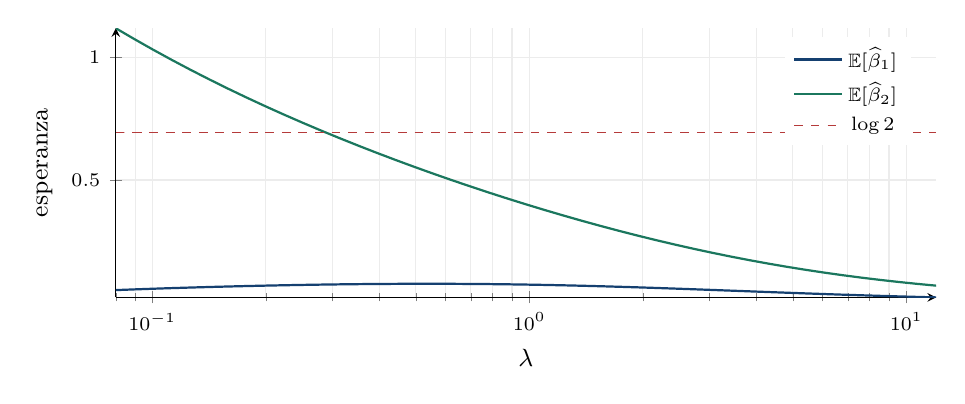
\begin{tikzpicture}
\begin{axis}[base,width=12cm,height=5cm,xmode=log,xmin=.08,xmax=12,xlabel={$\lambda$},ylabel={esperanza},legend pos=north east]
\addplot[azul,thick] coordinates {(0.080000000,0.0502589406) (0.089649239,0.0531606805) (0.100462325,0.0558612270) (0.112579637,0.0583768511) (0.126158485,0.0607202709) (0.141375152,0.0629006472) (0.158427184,0.0649237415) (0.177535956,0.0667921889) (0.198949542,0.0685058414) (0.222945937,0.0700621454) (0.249836670,0.0714565329) (0.279970841,0.0726828100) (0.313739660,0.0737335380) (0.351581521,0.0746004071) (0.393987697,0.0752746040) (0.441508714,0.0757471791) (0.494761502,0.0760094165) (0.554437401,0.0760532093) (0.621311137,0.0758714425) (0.696250881,0.0754583791) (0.780229519,0.0748100449) (0.874337282,0.0739246037) (0.979795897,0.0728027069) (1.097974455,0.0714478038) (1.230407177,0.0698663903) (1.378813335,0.0680681768) (1.545119575,0.0660661540) (1.731484923,0.0638765395) (1.940328817,0.0615185926) (2.174362519,0.0590142940) (2.436624309,0.0563878957) (2.730518933,0.0536653567) (3.059861800,0.0508736921) (3.428928516,0.0480402680) (3.842510393,0.0451920831) (4.305976649,0.0423550783) (4.825344112,0.0395535111) (5.407355334,0.0368094297) (6.059566123,0.0341422673) (6.790443632,0.0315685709) (7.609476286,0.0291018657) (8.527296962,0.0267526460) (9.555821023,0.0245284786) (10.708401014,0.0224341947) (12.000000000,0.0204721492)};\addplot[verde,thick] coordinates {(0.080000000,1.1198924486) (0.089649239,1.0753637045) (0.100462325,1.0323052798) (0.112579637,0.9906746395) (0.126158485,0.9504216173) (0.141375152,0.9114904124) (0.158427184,0.8738215773) (0.177535956,0.8373538860) (0.198949542,0.8020260060) (0.222945937,0.7677779291) (0.249836670,0.7345521466) (0.279970841,0.7022945760) (0.313739660,0.6709552597) (0.351581521,0.6404888658) (0.393987697,0.6108550222) (0.441508714,0.5820185134) (0.494761502,0.5539493679) (0.554437401,0.5266228558) (0.621311137,0.5000194142) (0.696250881,0.4741245088) (0.780229519,0.4489284396) (0.874337282,0.4244260896) (0.979795897,0.4006166170) (1.097974455,0.3775030866) (1.230407177,0.3550920360) (1.378813335,0.3333929741) (1.545119575,0.3124178104) (1.731484923,0.2921802154) (1.940328817,0.2726949194) (2.174362519,0.2539769606) (2.436624309,0.2360408968) (2.730518933,0.2189000060) (3.059861800,0.2025655011) (3.428928516,0.1870457915) (3.842510393,0.1723458263) (4.305976649,0.1584665504) (4.825344112,0.1454045043) (5.407355334,0.1331515869) (6.059566123,0.1216949947) (6.790443632,0.1110173352) (7.609476286,0.1010969021) (8.527296962,0.0919080908) (9.555821023,0.0834219215) (10.708401014,0.0756066383) (12.000000000,0.0684283452)};\addplot[rojo,dashed,domain=.08:12]{ln(2)};\legend{$\E[\widehat\beta_1]$,$\E[\widehat\beta_2]$,$\log2$}
\end{axis}
\end{tikzpicture}
\caption{Esperanzas finitas de ambos coeficientes y valor verdadero de la pendiente.}
\end{figure}

\begin{figure}[H]\centering
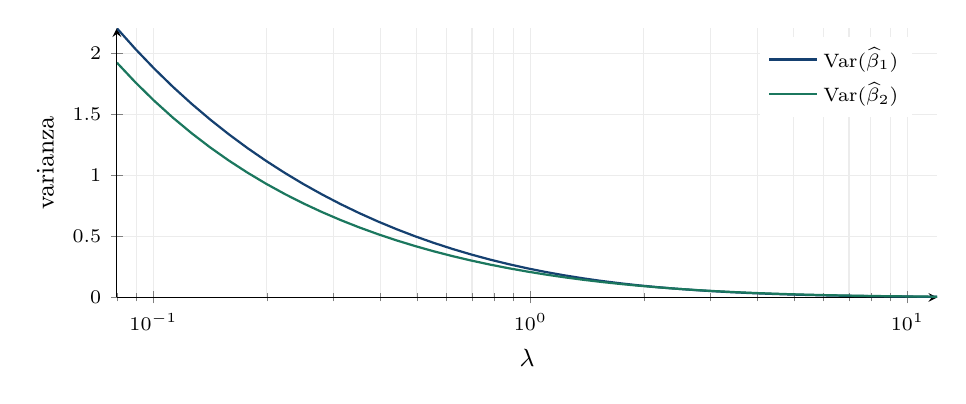
\begin{tikzpicture}
\begin{axis}[base,width=12cm,height=5cm,xmode=log,xmin=.08,xmax=12,ymin=0,xlabel={$\lambda$},ylabel={varianza},legend pos=north east]
\addplot[azul,thick] coordinates {(0.080000000,2.2040550887) (0.089649239,2.0331674379) (0.100462325,1.8737840278) (0.112579637,1.7251041837) (0.126158485,1.5863825097) (0.141375152,1.4569304672) (0.158427184,1.3361165208) (0.177535956,1.2233650230) (0.198949542,1.1181540310) (0.222945937,1.0200122576) (0.249836670,0.9285153495) (0.279970841,0.8432816713) (0.313739660,0.7639677520) (0.351581521,0.6902635307) (0.393987697,0.6218875207) (0.441508714,0.5585820001) (0.494761502,0.5001083295) (0.554437401,0.4462424959) (0.621311137,0.3967709821) (0.696250881,0.3514870598) (0.780229519,0.3101876004) (0.874337282,0.2726704907) (0.979795897,0.2387327199) (1.097974455,0.2081691821) (1.230407177,0.1807722011) (1.378813335,0.1563317489) (1.545119575,0.1346362864) (1.731484923,0.1154741168) (1.940328817,0.0986351166) (2.174362519,0.0839126873) (2.436624309,0.0711057734) (2.730518933,0.0600208008) (3.059861800,0.0504734154) (3.428928516,0.0422899323) (3.842510393,0.0353084424) (4.305976649,0.0293795529) (4.825344112,0.0243667711) (5.407355334,0.0201465597) (6.059566123,0.0166081054) (6.790443632,0.0136528529) (7.609476286,0.0111938567) (8.527296962,0.0091550011) (9.555821023,0.0074701359) (10.708401014,0.0060821671) (12.000000000,0.0049421378)};\addplot[verde,thick] coordinates {(0.080000000,1.9224489542) (0.089649239,1.7600225439) (0.100462325,1.6103164698) (0.112579637,1.4724231691) (0.126158485,1.3454651041) (0.141375152,1.2286040863) (0.158427184,1.1210482974) (0.177535956,1.0220569797) (0.198949542,0.9309429582) (0.222945937,0.8470732750) (0.249836670,0.7698682832) (0.279970841,0.6987995591) (0.313739660,0.6333869669) (0.351581521,0.5731951710) (0.393987697,0.5178298372) (0.441508714,0.4669337142) (0.494761502,0.4201827399) (0.554437401,0.3772822803) (0.621311137,0.3379635749) (0.696250881,0.3019804402) (0.780229519,0.2691062653) (0.874337282,0.2391313163) (0.979795897,0.2118603592) (1.097974455,0.1871105984) (1.230407177,0.1647099230) (1.378813335,0.1444954461) (1.545119575,0.1263123156) (1.731484923,0.1100127759) (1.940328817,0.0954554523) (2.174362519,0.0825048354) (2.436624309,0.0710309392) (2.730518933,0.0609091112) (3.059861800,0.0520199725) (3.428928516,0.0442494661) (3.842510393,0.0374889920) (4.305976649,0.0316356037) (4.825344112,0.0265922395) (5.407355334,0.0222679593) (6.059566123,0.0185781579) (6.790443632,0.0154447270) (7.609476286,0.0127961441) (8.527296962,0.0105674720) (9.555821023,0.0087002615) (10.708401014,0.0071423589) (12.000000000,0.0058476251)};\legend{$\Var(\widehat\beta_1)$,$\Var(\widehat\beta_2)$}
\end{axis}
\end{tikzpicture}
\caption{Varianzas finitas calculadas mediante todos los vectores de respuestas.}
\end{figure}

La penalización hace que las raíces se acerquen a cero.
Las ecuaciones implican la cota más directa
\[
|\widehat\beta_j|
\le\frac{\sum_i|x_{ij}|}{\lambda},
\]
porque cada discrepancia tiene valor absoluto a lo sumo uno.
Con diseño fijo, todos los coeficientes convergen
uniformemente a cero al crecer \(\lambda\).
Por ello las medias y las varianzas convergen a cero.
El sesgo de la pendiente, en cambio, converge a \(-\log2\).
Una variabilidad pequeña no garantiza un estimador
cercano al valor verdadero.
Estas curvas son resultados de este experimento;
no demuestran monotonicidad de cada varianza
para cualquier diseño.

\clearpage
\section{Comparar momentos finitos con una expansión local penalizada}\label{logit147}
Expandir la ecuación penalizada alrededor del parámetro verdadero
produce una regla lineal aproximada para el estimador:
\[
\begin{aligned}
\widehat\beta-\beta_\star\approx&
\left[
\sum_i\frac{e^{\sum_jx_{ij}\beta_{\star j}}}
{(1+e^{\sum_jx_{ij}\beta_{\star j}})^2}x_ix_i\T+I_2
\right]^{-1}\\
&\quad\cdot\left\{
\sum_i x_i\left[Y_i-
\frac{e^{\sum_jx_{ij}\beta_{\star j}}}
{1+e^{\sum_jx_{ij}\beta_{\star j}}}\right]
-\beta_\star\right\}.
\end{aligned}
\]
La parte del gradiente Bernoulli tiene esperanza cero;
la penalización produce un desplazamiento determinista.
Con las cuatro probabilidades verdaderas, la curvatura
sin penalización y la inversa penalizada son
\[
\sum_{i=1}^4\Prob(Y_i=1\mid X)\Prob(Y_i=0\mid X)x_ix_i\T=\begin{pmatrix}0.85444444&0.32000000\\0.32000000&1.08444444\end{pmatrix},
\]
\[
\left[\sum_{i=1}^4\Prob(Y_i=1\mid X)\Prob(Y_i=0\mid X)x_ix_i\T+I_2\right]^{-1}\approx\begin{pmatrix}0.55391883&-0.08503658\\-0.08503658&0.49279879\end{pmatrix}.
\]

La media y la covarianza de esa regla lineal aproximada
resultan, respectivamente,
\[
\E[\widehat\beta\mid X]\text{ por expansión local}\approx\begin{pmatrix}0.05894287\\0.35156509\end{pmatrix}.
\]
\[
\Cov(\widehat\beta\mid X)\text{ por expansión local}\approx\begin{pmatrix}0.23986154&0.00397271\\0.00397271&0.24271692\end{pmatrix}.
\]

La segunda matriz es un producto de tres factores:
inversa penalizada, curvatura Bernoulli, inversa penalizada.
No coincide con la inversa penalizada sola.
Los momentos de la raíz no lineal calculados
por enumeración fueron
\[
\E[\widehat\beta\mid X]\approx\begin{pmatrix}0.07257685\\0.39642252\end{pmatrix},\quad \Cov(\widehat\beta\mid X)\approx\begin{pmatrix}0.23301243&-0.00954533\\-0.00954533&0.20724398\end{pmatrix}.
\]

La diferencia puede atribuirse a los términos de orden
mayor que la expansión local omite.
La enumeración no necesita aproximar la raíz por una
función lineal de las respuestas.
Con una muestra mayor y penalización en escala adecuada,
la expansión puede proporcionar una buena aproximación;
con cuatro observaciones debe evaluarse, como se hizo aquí.

Hay así tres matrices distintas: la inversa de curvatura
penalizada, el producto local de tres factores,
y la covarianza finita de la regla completa.
Darles el mismo nombre sin especificar su interpretación
ocultaría una diferencia matemática concreta.

\clearpage
\section{Derivar la trayectoria de ridge respecto de su intensidad}\label{logit148}
Para un vector de respuestas fijo, la raíz penalizada
depende suavemente de \(\lambda>0\).
Su curvatura positiva es invertible porque incluye
\(\lambda I_k\). Diferenciemos la ecuación
\[
\sum_i x_i\left[y_i-
\frac{e^{\sum_jx_{ij}\widehat\beta_{\lambda j}}}
{1+e^{\sum_jx_{ij}\widehat\beta_{\lambda j}}}\right]
-\lambda\widehat\beta_\lambda=0.
\]
El primer término cambia a través de los coeficientes.
El segundo tiene dos derivadas por la regla del producto:
\(-\widehat\beta_\lambda-\lambda\dd\widehat\beta_\lambda/\dd\lambda\).
Reunir los términos da
\[
\frac{\dd\widehat\beta_\lambda}{\dd\lambda}
=-\left[
\sum_i\frac{e^{\sum_jx_{ij}\widehat\beta_{\lambda j}}}
{(1+e^{\sum_jx_{ij}\widehat\beta_{\lambda j}})^2}
x_ix_i\T+\lambda I_k
\right]^{-1}\widehat\beta_\lambda.
\]
La derivada de cada coordenada mezcla todas las
coordenadas mediante esa inversa.
No tiene por qué ser siempre opuesta al signo
de la misma coordenada del coeficiente.

En cambio, la norma al cuadrado sí tiene una
derivada de signo controlado:
\[
\begin{aligned}
\frac{\dd}{\dd\lambda}\|\widehat\beta_\lambda\|_2^2
&=2\widehat\beta_\lambda\T
\frac{\dd\widehat\beta_\lambda}{\dd\lambda}\\
&=-2\widehat\beta_\lambda\T
\left[
\sum_i\frac{e^{\sum_jx_{ij}\widehat\beta_{\lambda j}}}
{(1+e^{\sum_jx_{ij}\widehat\beta_{\lambda j}})^2}
x_ix_i\T+\lambda I_k
\right]^{-1}\widehat\beta_\lambda\le0.
\end{aligned}
\]
La desigualdad es estricta cuando la raíz es no nula.
Se apoya en positividad de la inversa completa,
no en el signo de sus entradas individuales.

La trayectoria depende de penalizar todas las coordenadas.
Si se excluye el intercepto, cambia la matriz de penalización
y cambian tanto las condiciones de existencia como la identidad.
Un descenso de la norma tampoco prueba por sí solo
un descenso de cada error cuadrático.
El sesgo frente al parámetro verdadero debe
seguirse estudiando mediante los momentos correspondientes.

La derivada implícita permite predecir la raíz en una
intensidad cercana, pero luego se deben resolver y
verificar otra vez las ecuaciones del gradiente.
Usar solo la predicción lineal a una distancia grande
sería otra aproximación.

\clearpage
\section{Reproducir los cálculos sin saltar el control numérico}\label{logit149}
La regla de cálculo utilizada en los laboratorios
puede expresarse como una secuencia matemática verificable.
Se comienza con \(\beta^{(0)}=0\).
Para cada iteración se evalúan todas las probabilidades
con la misma versión de los coeficientes:
\[
\frac{e^{\sum_jx_{ij}\beta_j^{(m)}}}
{1+e^{\sum_jx_{ij}\beta_j^{(m)}}},\quad i=1,\ldots,n.
\]
Después se construyen, por sumas de filas,
\[
\sum_i x_i\left[y_i-
\frac{e^{\sum_jx_{ij}\beta_j^{(m)}}}
{1+e^{\sum_jx_{ij}\beta_j^{(m)}}}\right]-\lambda\beta^{(m)}
\]
y
\[
\sum_i\frac{e^{\sum_jx_{ij}\beta_j^{(m)}}}
{(1+e^{\sum_jx_{ij}\beta_j^{(m)}})^2}x_ix_i\T+\lambda I_k.
\]
Se resuelve el sistema cuyo lado izquierdo es
esta última matriz por \(\Delta^{(m)}\),
y cuyo lado derecho es el vector anterior.
Para el modelo ordinario se toma \(\lambda=0\),
después de comprobar existencia y rango.

La propuesta \(\beta^{(m)}+\Delta^{(m)}\) se evalúa
en el objetivo original. Si no satisface el criterio
de ascenso, se reduce el paso sucesivamente.
El cálculo estable de cada logaritmo usa
\[
\log(1+e^t)=\max(t,0)+\log(1+e^{-|t|}),
\]
con \(t\) igual al producto lineal que se está evaluando.
Esta identidad evita desbordamientos sin alterar la función.

Al finalizar, se verifican tres propiedades distintas:
el residuo del sistema lineal, el gradiente del objetivo
en la nueva raíz y el cambio del valor del objetivo.
En el experimento finito también se verifica que
las dieciséis masas sumen uno y que la covarianza
calculada por segundos momentos coincida con la
suma de productos de vectores centrados.

Todos los números de las tablas fueron obtenidos
con cálculo interno en doble precisión y redondeados
solo para su impresión.
Los valores numéricos que dependen de raíces se expresan
como aproximaciones; las identidades algebraicas
y las fracciones de probabilidades se conservan como tales.

Las figuras están dibujadas con TikZ y PGFPlots dentro
del mismo archivo. No requieren descargar imágenes
ni mantener una carpeta adicional de datos para compilar.
El archivo conserva el control de compilación en la
receta que ya funciona en VS Code.

\clearpage
\section{Fuentes primarias y alcance de las demostraciones}\label{logit150}
Las derivaciones de este documento se presentan con
los datos y las expresiones abiertas.
Las fuentes siguientes permiten ampliar la teoría
de modelos lineales generalizados, optimización convexa,
econometría e inferencia en presencia de separación.

El cálculo de verosimilitud Bernoulli y su enlace logístico
puede contrastarse con las notas de Stanford.
La concavidad, la búsqueda de paso y Newton tienen
un tratamiento sistemático en el libro de Boyd y Vandenberghe.
La teoría de estimadores y covarianzas asintóticas
se desarrolla en el texto de Hansen.
Los trabajos originales de Firth y de Heinze y Schemper
se refieren a ajustes de sesgo y separación.

Las pruebas finitas y asintóticas requieren hipótesis distintas.
En particular, existencia en una realización, consistencia
de un estimador y existencia de su esperanza finita
son afirmaciones diferentes.
Las unidades dedicadas a esos puntos explicitan
qué problema está resolviendo cada argumento.

\begin{thebibliography}{9}
\bibitem{stanford}
Andrew Ng y Tengyu Ma.
\emph{CS229: Supervised Learning}, notas del curso, primavera de 2020.
\url{https://cs229.stanford.edu/notes2020spring/cs229-notes1.pdf}.
\bibitem{boyd}
Stephen Boyd y Lieven Vandenberghe.
\emph{Convex Optimization}, Cambridge University Press, 2004.
Material de los autores:
\url{https://web.stanford.edu/~boyd/cvxbook/}.
\bibitem{hansen}
Bruce E. Hansen.
\emph{Econometrics}, Princeton University Press, 2022.
Material del autor:
\url{https://users.ssc.wisc.edu/~behansen/econometrics/}.
\bibitem{firth}
David Firth.
Bias reduction of maximum likelihood estimates.
\emph{Biometrika}, 80(1), 27--38, 1993.
\url{https://doi.org/10.1093/biomet/80.1.27}.
\bibitem{heinze}
Georg Heinze y Michael Schemper.
A solution to the problem of separation in logistic regression.
\emph{Statistics in Medicine}, 21(16), 2409--2419, 2002.
\url{https://doi.org/10.1002/sim.1047}.
\end{thebibliography}

\end{document}
